\newcommand{\ResourceCaseCaption}{Exact oracle replay of \texttt{roadster-\allowbreak{}body-\allowbreak{}05} from source 31027. The displayed operations are 0, 14, 28, 42; the certified optimum is 42 operations. This is a software witness, not a model trajectory.}
\newcommand{\GeometryCaseCaption}{Primary inventory-matched pair \texttt{source-\allowbreak{}v23-\allowbreak{}10037-\allowbreak{}matched-\allowbreak{}0/\allowbreak{}geometry/\allowbreak{}future-\allowbreak{}00} from held-out source 10037 in the initial isometric view. Both contexts use 63 source pieces (47 fixed); the exact part-number/color multiset, registered poses, start, target, rack, work, and plan match. After 2 shared legal operations, the exact labels are context 1: first conflict at operation 3; context 2: all legal. Only subsets of original fixed instances change. These publication views omit ID overlays; answers are evaluator annotations. Pixel distinction is not perceptual answerability.}
\newcommand{\RepairCaseCaption}{Certified lag-5 repair, \texttt{source-\allowbreak{}10036-\allowbreak{}35/\allowbreak{}repair-\allowbreak{}lag-\allowbreak{}5}, source 10036. A: the pre-error checkpoint defines the optimal corridor. B: an error and 5 further operations leave it. The last history action is \texttt{attach P013}. Undoing it first requires 9 operations to repair; the optimum takes 7, starting with \texttt{detach P002}. C: a nonterminal corridor state is restored. These are oracle replay frames, not model reasoning or a model success; exact source instances and actions are archived.}

\section{Exact labels and admissible bounds}
The archived predecessor audit evaluates every stored nonnegative
state--goal label. Let $R$ be occupied blocker closure for required
removals and insertions. Without capacity or inspection obligations, the
formula $|A\triangle G|+2|R\cap A\cap G|$ agrees with all
\OldLabels{} audited labels. This is a finite-census equality, not a
general theorem about arbitrary assembly domains or visual perception.

For BrickPlan's lower bound, initially mismatched sites each require an
operation. Every occupied target site in the required removal closure
must be detached and reattached. Every unfinished job needs one audit.
These counts refer to disjoint required operations. Recursively including
occupied path blockers can only add necessary removals. Ignoring capacity
scheduling and some connectivity effects relaxes the problem, so
$h(x)\leq C^*(x)$. The verifier checks this inequality at every oracle node.

For every nonterminal product node, the certificate checks
$C^*(x)=\min_{a\in A(x)}[1+C^*(T(x,a))]$, with terminal cost zero.
Physical edges are compared with independent runtime transition
enumeration and inverse execution; audit edges are replayed as well.
Every retained product state reaches a terminal. The physical graph is
reversible within its capacity-constrained component. Audits add a
persistent bit without removing a physical action, and all admitted jobs
can be exposed. Consequently, legal successors do not become genuine
irreversible dead ends. Budget exhaustion and extra cost remain possible.

\section{Construction details}
The frozen candidate registry and source plan fix new kit identities,
intake strata, hash-assigned source-group splits, geometry admission rules,
and task sampling before qualification or solver discovery. The exact
registry hash is archived. New admissions require at least eight registered
and eight reachable movable sites; legacy smaller domains remain historical.
Deterministic source-order endpoint pruning and bounded stud-connected
extraction retain original instance identities and transforms. The
predecessor's earlier pruning refinement remains disclosed in its frozen
record; it is not retroactively called preregistered.

Independent original-MPD hierarchy and identity audits are an additional
release gate. They exclude kits 10124, 10226, 10261, 10262 and 21318 because
their part-only manifests omit direct model geometry, and kit 30312 because
its original root identifies a different kit. These exclusions follow the
initial geometric qualification and do not depend on policy performance.
The earlier admissions and unchanged original files are archived.
Every retained new-source part's index and instance ID are bound to its exact
original reference chain, part/color identity and composed matrix.
Failed downloads remain acquisition exclusions, without claims that the
official models themselves are defective.

Each newly admitted source contributes \GoalsPerSource{} goals,
\JobSettingsPerSource{} job settings (zero, two, and four inspections),
and \StartsPerMission{} seeded nonterminal starts per mission.
The goal is either the full assembly or a seeded supported partial target.
The rack holds $\lceil0.6|V|\rceil$ pieces. Reachability, not cost, gap,
policy performance, or expansion count, admits tasks. Easy episodes
remain included. Geometry contrasts are a separate mechanism-conditioned
diagnostic, not part of this source-sampling factorial.

Primary matched contexts are induced by deleting one or two original fixed
instances from each side. Geometry-only enumeration groups deletions by
exact part-number/color inventory, keeps distinct support masks, and selects
at most four context pairs per base in seeded hash order. It never moves
pieces, adds spacers, substitutes meshes, or falls back to unequal counts.
Both fixed structures remain connected and the full assemblies supported;
endpoint and straight-path qualification are recomputed. Registered
instances, poses, start, goal, capacity, jobs, and proposed plan match.

After this selection, a bounded differing-edge search seeks exact optimal
completions with a shared legal prefix of at least two operations.
At most two distinct starting questions are retained per intervention.
Of \QualifiedInterventionCount{} qualified primary interventions,
\ZeroYieldInterventionCount{} yield no retained pair. This is search-specific
attrition, not proof that other contrasts cannot exist. The retained
\PrimaryPairCount{} pairs and \HistoricalPairCount{} unmatched historical
regressions have separate denominators. Original/grayscale controls preserve
all geometry and labels.

The \SequencePairCount{} interior-order pairs are balanced over conflict bins 2--5,
6--10, and 11+. Legal and reordered plans share exact prefixes up to
the first conflict, endpoints, and action multisets. Legal witnesses
have no repeated states. The stored audit exposes each conflict position,
so readers can run other prefix controls.

\begin{table}[t]
\centering\small
\caption{A prefix-only software control returns the first conflict if
it appears within $k$ executed operations, otherwise ``all legal.''
The denominator is all \ContinuationCount{} continuation questions.}
\begin{tabular}{rrr}\toprule
Prefix length & Correct / assigned & Accuracy\\\midrule
0 & 216/432 & 50.0\%\\
1 & 216/432 & 50.0\%\\
2 & 234/432 & 54.2\%\\
3 & 257/432 & 59.5\%\\
5 & 288/432 & 66.7\%\\
8 & 340/432 & 78.7\%\\
11 & 372/432 & 86.1\%\\
16 & 410/432 & 94.9\%\\
24 & 426/432 & 98.6\%\\
32 & 432/432 & 100.0\%\\
\bottomrule\end{tabular}

\end{table}

\section{Shallow choice and control diagnostics}
\begin{table}[t]
\centering\small
\caption{Measured finite-horizon choice sets for all \NextActionCount{} next-action
questions. Any/all refer to optimistic/pessimistic ties; uniform tie
correctness is an exact average, not a sampled policy result.}
\begin{tabular}{rrrrr}\toprule
Depth & Choices & \shortstack{All\\optimal} & \shortstack{Any\\optimal} & \shortstack{Uniform\\tie}\\\midrule
1 & 2595 & 2445 & 2595 & 97.4\%\\
2 & 2595 & 2484 & 2595 & 98.1\%\\
4 & 2595 & 2505 & 2595 & 98.3\%\\
8 & 2595 & 2544 & 2595 & 99.0\%\\
\bottomrule\end{tabular}

\end{table}
The depth-one minimizing set contains an optimal action at
\DepthOneContainsOptimal{} of \NextActionCount{} selected checkpoints.
These privileged structural choices do not establish a required internal
reasoning depth for image-input policies.
Deeper horizons can change tie composition nonmonotonically. The full
table is retained without redefining difficulty to match its results.

\begin{table*}[t]
\centering\small
\caption{Structural policy completion by operation-length bin.
Each nonoracle policy has three tie-order seeds per episode.}
\begin{tabular}{lrrrr}\toprule
Control & D1 & D2 & D3 & D4\\\midrule
Closure greedy & 942/942 & 2096/2103 & 988/1023 & 137/195\\
Capacity dispatch & 942/942 & 2097/2103 & 970/1023 & 123/195\\
Closure A* (100) & 942/942 & 2088/2103 & 946/1023 & 99/195\\
Closure A* (1,000) & 942/942 & 2103/2103 & 1005/1023 & 149/195\\
Closure A* (full) & 942/942 & 2103/2103 & 1023/1023 & 195/195\\
Hamming A* (full) & 942/942 & 2103/2103 & 1023/1023 & 195/195\\
\bottomrule\end{tabular}

\end{table*}
All \RawPolicyRuns{} raw policy task-run records are archived in
\texttt{data/software-control-records.json.gz}. They include one oracle
seed and three seeds for nine other policies, with actions, outcomes,
expansions, timings, and regrets. The release checker recomputes every
overall, tier, source, and seed aggregate. The full search cap of
500,000 is a resource ceiling, not actual expansion usage. Oracle loading
and cached local timing are not comparable to calibrated online search.

\section{Recovery, diagnosis, and censoring}
Traverse only edges with $C^*(T(x,a))=C^*(x)-1$ from pre-error state
$b$. The reached states are exactly the union of optimal completions:
each traversal is an optimal prefix, and every optimal prefix satisfies
that equality. Remove the terminal state to obtain the repair target
$\mathcal C_b^{-}$. The generator's delayed checkpoints remain outside
this set after an error and lag 1, 3, or 5. Independent forward BFS
verifies their shortest return distances, which range from
\RepairMin{} to \RepairMax{}. Lag-specific denominators for the
\RepairCount{} questions appear below.

\begin{table}[t]
\centering\small
\caption{Delayed-repair lag and public inverse-last control.}
\begin{tabular}{rrrr}\toprule
Lag & Questions & Inverse correct & Accuracy\\\midrule
1 & 1309 & 919 & 70.2\%\\
3 & 1268 & 715 & 56.4\%\\
5 & 1252 & 626 & 50.0\%\\
\bottomrule\end{tabular}

\end{table}

Each positive-excess legal action creates its own spontaneous event;
later actions update every active event. A second error never replaces
the first. Immediate recovery and lag-specific delayed cohorts are
reported separately. Unfinished events are censored; terminal events
that never restore a nonterminal corridor state are observed failures.
Reaching a goal after a costly detour earns completion credit, but not
automatic corridor-repair credit.

The inverse-last-action control uses only the public executed history
and candidate list. It earns zero when no inverse is offered.
Its combined \InverseCorrect{}/\RepairCount{} accuracy is
\InverseAccuracy{}. There are \InverseSuboptimal{} cases with a legal
but suboptimal inverse and \InverseUnavailable{} with no offered inverse. Lag is thus an
experimental descriptor, not proof of necessary nonlocal reasoning.

There are \CalibrationCount{} all-correct-choice calibration questions across the
diagnostic bank. Their correct tie sets are preserved, and the evaluator
reports calibration separately from the \DiscriminativeCount{} discriminative rows.
The \ProbeCount{} rows map to \ProblemCount{} canonical problems. Assigned repeated variants
are averaged before problems and sources; missing responses receive
zero before this averaging. The evaluator exposes both row and clustered
scores, plus each inverse-control cohort. None of these private labels
is included in the policy observation.

\begin{table}[t]
\centering\small
\caption{Recovery cohorts are not pooled into a claim of nonlocal repair.}
\begin{tabular}{lrrr}\toprule
Inverse cohort & Questions & Sources & Repair cost\\\midrule
Optimal inverse & 2260 & 97 & 2--13\\
Suboptimal inverse & 1487 & 96 & 1--7\\
No offered inverse & 82 & 44 & 1--11\\
\bottomrule\end{tabular}

\end{table}

An accepted diagnosis concerns legal positive-excess events since the
last diagnosis or episode start. The first later diagnosis is attached
to each previously undiagnosed event, with its sign and lag. True
positive diagnosis checkpoints open replanning-suffix records.
Always-negative or selectively requested diagnoses can yield misleading
accuracy, so report event detection and query coverage alongside it.

Plan-survival reports retain the first cost loss even after recovery,
and include explicit eligible/observed/unknown counts per operation index.
They are descriptive task-budget curves, not Kaplan--Meier population
estimates. Conditions should use matched assignments and registered
source strata. Missing episodes must not disappear from denominators.

\subsection{Regret conservation}
For a successful trace, accepted attaches $A_c$ and detaches $D_c$
satisfy $A_c-D_c=\Delta$, the target-minus-start occupancy count.
There are exactly $u$ accepted previously unfinished audits.
Duplicate audits are rejected. If $N_{\rm invalid}$ is the number of
charged invalid attempts, then
\begin{align}
T &=2D_c+\Delta+u+N_{\rm invalid},\\
C^*(x_0)&=2D^*+\Delta+u,\\
T-C^*(x_0)&=2(D_c-D^*)+N_{\rm invalid}.
\end{align}
This audit-inclusive identity reconciles detachment regret and total
excess. Rejected actions consume budget; stale HTTP revisions and malformed
request envelopes are rejected before mutation and are not action events.

\section{Visual stimuli and actual model calls}
All executable geometry uses original source poses and LDraw triangle
meshes. The \MeshCount{} distinct part meshes contain \TriangleCount{} triangles.
\texttt{ASSET-LICENSES.json} preserves source models, authors, URLs, and
part-level notices; attribution and licenses remain separate from code.
Qualification proxies do not replace the displayed shapes.
Figure provenance records exact states, seeds, bank hash, and image hashes.

The public renderer supersamples by two before Lanczos downsampling to
native HD. Display canvases account for device-pixel ratio, and native
zoom avoids CSS-only enlargement of low-resolution pixels.
Catalog tiles are $480\times360$ and catalogs are 1920 pixels wide.
Models receive image content, not text describing images. Preprocessing
is separately declared: the local SmolVLM case resizes to longest edge
512, with splitting disabled. HD display does not imply native-HD model
processing.

The preserved version-2.1 local case contains four actual inference calls
on historical public E069, seed 0. The original task and bank hash are
archived; this trace is not relabeled as version-2.3 evaluation.
All calls return descriptive prose instead of an executable JSON action.
The executor rejects each, and the controller stops at its four-call limit.
Every prompt, raw response, image hash, latency, measured token count,
action, and feedback is archived. No oracle action or fabricated explanation
replaces model output. This is a failed integration example. It supplies
neither an estimate of SmolVLM accuracy nor evidence about larger VLMs.

\section{Protocol and reproducibility}
Study runs bind participant, condition, seed, assignments, and bank hash.
The evaluator replays mutations, validates views, and normalizes candidate
permutations. Retries are idempotent across restart; changed content or
stale revisions are rejected. Failed atomic persistence rolls back mutations.

Practice exposes rich catalogs, solution review after submission, and
free 3D inspection. Study mode blocks these and private downloads.
Portable evaluator data must remain on the evaluator host during blind
studies; a local working-directory convention is not a security sandbox.

The practice model manager supports local MLX and OpenAI-compatible
vision calls, durable outputs, and bounded run/step/stop. Credentials
never enter browser exports. Stop prevents subsequent actions, not
in-flight provider billing. Interrupted calls are never silently retried.

The population study runner is distinct. Its reported-usage mode reserves
maximum tokens and cost before calls; adapters account for images and
attest usage. Missing accounting, timeout, malformed responses, or limit
violations stop continuation. Unavailable-accounting mode marks tokens
and currency unavailable. This relies on adapter/provider reports, not
a provider-enforced spending quota.

The main paper uses the unmodified official CVPR author-kit, pinned to
commit \texttt{2917585}, labeled 2026. A future year's kit is not claimed.
The PDF uses public preprint mode without margin/font compression.
Review mode requires the actual year and paper ID.

\clearpage
\onecolumn
\begin{center}
\small
\captionof{table}{Metric denominators and treatment of missing outcomes.}
\begin{tabular}{p{.22\textwidth}p{.38\textwidth}p{.30\textwidth}}\toprule
Metric & Eligible denominator & Missing / termination rule\\\midrule
Completion / optimal completion & All assigned episodes & Unstarted and unfinished are failures\\
Successful mean regret & Successfully finished episodes & Null for failures; report success coverage\\
Avoidable-cost choice & Legal decisions with zero- and positive-excess alternatives & Invalid attempts excluded here, charged in total\\
Budget-loss choice & Viable checkpoints with viable and nonviable legal choices & Other budget losses remain in raw records\\
True-unreachability choice & No eligible choices in retained components & Undefined, not empirical evidence of zero risk\\
Recovery bounds & Every eligible legal positive-excess event & Lower bound restored/all; upper adds censored\\
Diagnosis accuracy & Accepted diagnosis queries & Unqueried intervals are not inferred correct\\
Primary geometry joint correctness & Pairs with at least one assigned member & Both exact labels required; absent partner scores zero\\
Discriminative probe accuracy & Assigned noncalibration questions of that family & Missing or invalid response gets no credit\\
Source macro accuracy & Variants within problem, then problems within source, then sources & Missing variants enter as zero before averaging\\
Calibration accuracy & Assigned all-correct-choice questions & Report separately; not evidence of discrimination\\
\bottomrule\end{tabular}
\end{center}

\section{Base source assemblies}
The table lists \BaseProfileCount{} base assemblies; roadster and kart
share kit 31027. An additional \ContextProfileCount{} qualified context profiles are indexed
in the machine-readable source census. They are not independent sources.
Profiles without episodes are zero-yield candidates, not benchmark tasks.
There are \ZeroYieldProfileCount{} profiles without episodes.
Registered and movable counts describe different quantities; ``Parts''
counts the admitted subassembly, not the full original kit.
The active bank covers \SourceCount{} source groups.
\begingroup\small
\begin{longtable}{p{.32\textwidth}llrrrr}\toprule
Admitted subassembly & Kit & Split & Parts & Sites & Movable & Episodes\\\midrule
\endfirsthead
\toprule
Admitted subassembly & Kit & Split & Parts & Sites & Movable & Episodes\\\midrule\endhead
\midrule\endfoot
\bottomrule\endlastfoot
Roadster body & 31027 & Dev. & 37 & 17 & 17 & 14\\
Kart deck & 31027 & Dev. & 25 & 18 & 18 & 14\\
Airframe & 31028 & Dev. & 24 & 21 & 21 & 14\\
Truck cab and roof & 10156 & Dev. & 76 & 18 & 18 & 10\\
House roof assembly & 31009 & Dev. & 221 & 18 & 17 & 14\\
Sports car upper body & 5867 & Dev. & 149 & 22 & 10 & 3\\
Source 10001 subassembly & 10001 & Dev. & 17 & 2 & 2 & 8\\
Source 10159 subassembly & 10159 & Dev. & 177 & 16 & 16 & 12\\
Source 10220 subassembly & 10220 & Dev. & 153 & 16 & 16 & 12\\
Source 10014 subassembly & 10014 & Held out & 71 & 16 & 15 & 12\\
Source 10128 subassembly & 10128 & Held out & 98 & 16 & 14 & 12\\
Source omr-31031 subassembly & 31031 & Held out & 42 & 12 & 12 & 12\\
Source 10036 subassembly & 10036 & Held out & 79 & 16 & 16 & 48\\
Source 10213 subassembly & 10213 & Held out & 179 & 2 & 2 & 28\\
Source omr-10242 subassembly & 10242 & Held out & 180 & 16 & 16 & 48\\
Source omr-10265 subassembly & 10265 & Held out & 179 & 4 & 4 & 48\\
Source omr-10269 subassembly & 10269 & Held out & 105 & 16 & 11 & 48\\
Breezeway Cafe & 10037 & Held out & 65 & 16 & 12 & 12\\
Town Plan & 10184 & Held out & 96 & 16 & 16 & 12\\
Gingerbread House & 10267 & Held out & 96 & 16 & 16 & 12\\
Holiday Home & 1472 & Held out & 89 & 16 & 14 & 12\\
Weetabix Town House & 1484 & Held out & 96 & 16 & 16 & 12\\
Town Bank & 1490 & Held out & 92 & 16 & 16 & 12\\
House with Roof-Windows ( Velux ) & 1854 & Dev. & 92 & 16 & 16 & 12\\
The Big Bang Theory & 21302 & Held out & 96 & 16 & 15 & 12\\
Central Perk & 21319 & Held out & 96 & 16 & 16 & 12\\
Medieval Blacksmith & 21325 & Held out & 95 & 16 & 16 & 12\\
Mountain Hut & 31025 & Held out & 95 & 16 & 16 & 12\\
Changing Seasons & 31038 & Dev. & 94 & 16 & 16 & 12\\
Lakeside Lodge & 31048 & Dev. & 96 & 16 & 16 & 12\\
Beachside Vacation & 31063 & Dev. & 95 & 16 & 16 & 12\\
Burger Stand & 6683 & Held out & 50 & 16 & 16 & 12\\
Post-Station & 6689 & Held out & 39 & 16 & 16 & 12\\
Cycle Fix-It Shop & 6699 & Held out & 44 & 16 & 16 & 12\\
Solomon R. Guggenheim Museum & 21004 & Held out & 95 & 16 & 16 & 12\\
Fallingwater & 21005 & Held out & 96 & 16 & 16 & 12\\
The White House & 21006 & Dev. & 96 & 16 & 16 & 12\\
Rockefeller Center & 21007 & Dev. & 46 & 16 & 16 & 12\\
Farnsworth House & 21009 & Held out & 94 & 16 & 16 & 12\\
Robie House & 21010 & Held out & 87 & 16 & 16 & 12\\
Brandenburg Gate & 21011 & Dev. & 91 & 16 & 16 & 12\\
Sydney Opera House & 21012 & Dev. & 48 & 16 & 16 & 12\\
Villa Savoye & 21014 & Held out & 96 & 16 & 16 & 12\\
Sungnyemun & 21016 & Held out & 95 & 16 & 16 & 12\\
Imperial Hotel & 21017 & Held out & 96 & 16 & 16 & 12\\
United Nations Headquarters & 21018 & Dev. & 60 & 16 & 16 & 12\\
The Trevi Fountain & 21020 & Held out & 96 & 16 & 16 & 12\\
Lincoln Memorial & 21022 & Held out & 96 & 16 & 16 & 12\\
Louvre & 21024 & Held out & 96 & 16 & 16 & 12\\
Buckingham Palace & 21029 & Held out & 76 & 16 & 16 & 12\\
United States Capitol Building & 21030 & Held out & 92 & 16 & 16 & 12\\
LEGO House & 21037 & Held out & 96 & 16 & 16 & 12\\
Trafalgar Square & 21045 & Dev. & 83 & 16 & 16 & 12\\
Alligator & 20015 & Dev. & 13 & 12 & 11 & 12\\
Clown Fish & 30025 & Held out & 29 & 16 & 16 & 12\\
Panda & 30026 & Dev. & 15 & 14 & 14 & 12\\
Reindeer & 30027 & Dev. & 25 & 16 & 15 & 12\\
Pudsey Bear & 30029 & Held out & 64 & 16 & 16 & 12\\
Cute Pug & 30542 & Held out & 26 & 16 & 16 & 12\\
Pelican & 30571 & Dev. & 25 & 16 & 16 & 12\\
Space Shuttle & 1682 & Held out & 30 & 12 & 11 & 12\\
Jet & 1775 & Held out & 44 & 15 & 15 & 12\\
Light Aircraft and Ground Support & 1808 & Held out & 27 & 16 & 16 & 12\\
International Space Station & 21321 & Held out & 91 & 16 & 16 & 12\\
Helicopter & 30181 & Held out & 27 & 8 & 8 & 12\\
Swamp Police Helicopter & 30311 & Held out & 27 & 16 & 15 & 12\\
Blue Power Jet & 31039 & Dev. & 93 & 16 & 16 & 12\\
Twin Spin Helicopter & 31049 & Held out & 87 & 15 & 15 & 12\\
Space Shuttle Explorer & 31066 & Held out & 93 & 16 & 16 & 12\\
Helicopter Adventure & 31092 & Dev. & 60 & 16 & 16 & 12\\
Passenger Plane & 3181 & Dev. & 11 & 10 & 10 & 12\\
Propellor Power & 6745 & Held out & 94 & 16 & 16 & 12\\
WALL\textbullet{}E [Original Version] & 21303 & Held out & 33 & 14 & 11 & 12\\
Mobile Car Crane & 1489 & Held out & 93 & 8 & 8 & 12\\
Super Tow Truck & 1572 & Dev. & 63 & 16 & 16 & 12\\
Loader Tractor & 1633 & Dev. & 13 & 12 & 9 & 12\\
Pirate Roller Coaster & 31084 & Held out & 96 & 12 & 12 & 12\\
Repair Truck & 3179 & Dev. & 60 & 16 & 16 & 12\\
Pneumatic Crane & 6678 & Dev. & 16 & 15 & 12 & 12\\
Cement Mixer & 6682 & Held out & 20 & 16 & 16 & 12\\
Snorkel Pumper & 6690 & Held out & 25 & 16 & 16 & 12\\
Ferrari F40 & 10248 & Held out & 92 & 12 & 11 & 12\\
London Bus & 10258 & Held out & 9 & 8 & 8 & 12\\
Fiat 500 & 10271 & Dev. & 33 & 8 & 8 & 12\\
Adventure Vehicles & 31037 & Held out & 96 & 16 & 16 & 12\\
Desert Racers & 31040 & Dev. & 49 & 16 & 16 & 12\\
Turbo Track Racer & 31070 & Dev. & 96 & 16 & 16 & 12\\
Extreme Engines & 31072 & Held out & 56 & 12 & 12 & 12\\
LEGO Truck & 3221 & Held out & 91 & 16 & 16 & 12\\
Highway Transport & 6753 & Held out & 96 & 16 & 16 & 12\\
High Speed Train Car & 10158 & Dev. & 50 & 8 & 8 & 12\\
Emerald Night & 10194 & Held out & 90 & 12 & 12 & 12\\
Horizon Express & 10233 & Held out & 96 & 16 & 16 & 12\\
Maersk Line Triple-E & 10241 & Held out & 96 & 16 & 16 & 12\\
Ocean Explorer & 31045 & Held out & 96 & 16 & 16 & 12\\
Ship & 4018 & Held out & 9 & 8 & 8 & 12\\
RV with Speedboat & 6698 & Held out & 36 & 16 & 13 & 12\\
Motor Boat & 1632 & Dev. & 11 & 8 & 8 & 12\\
\end{longtable}

\endgroup
\begin{center}\small
\begin{tabular}{lrrrr}\toprule
Partition & Sources & Episodes & Greedy & Full A*\\\midrule
Development & 34 & 445 & 95.9\% & 100.0\%\\
Held-out source & 63 & 976 & 98.5\% & 100.0\%\\
\bottomrule\end{tabular}

\end{center}
Version 2.3 admits \AdmittedCount{} of \CandidateCount{} new frozen
candidates. All \RejectedCount{} rejected candidates remain documented.
All earlier episode and diagnostic definitions are preserved, without
promoting historical unmatched pairs to primary matched evidence.

\section{Source strata and admission attrition}
\begin{center}\small
\begin{tabular}{lrrrrrr}\toprule
Frozen intake stratum & Candidates & Admitted & Rejected & Held out & Pairs & Pair sources\\\midrule
aircraft-and-space & 16 & 12 & 4 & 9 & 0 & 0\\
animals & 11 & 7 & 4 & 3 & 0 & 0\\
architecture & 20 & 19 & 1 & 13 & 2 & 1\\
buildings-and-scenes & 20 & 17 & 3 & 13 & 18 & 5\\
mechanisms-and-working-vehicles & 12 & 9 & 3 & 5 & 2 & 1\\
rail-and-water & 10 & 8 & 2 & 6 & 4 & 1\\
road-vehicles & 11 & 9 & 2 & 6 & 0 & 0\\
\bottomrule\end{tabular}

\end{center}
Strata are frozen intake categories, not post hoc difficulty labels.
``Held out'' counts admitted new sources assigned to the held-out split;
``Pairs'' and ``Pair sources'' describe retained primary geometry only.
The following candidate census includes every frozen admission outcome.
Exact rejection reasons, pruned instances, qualification attempts, original
source URLs and authors, and dependency hashes remain in
\texttt{source-plan.json}, \texttt{data/source-admission.json}, and
\texttt{data/source-question-audit.json}.
\begingroup\small
\begin{longtable}{lllp{.28\textwidth}l}\toprule
Model & Kit & Split & Frozen stratum & Admission\\\midrule
\endfirsthead
\toprule
Model & Kit & Split & Frozen stratum & Admission\\\midrule\endhead
\midrule\endfoot
\bottomrule\endlastfoot
v23-10037 & 10037 & Held out & buildings-and-scenes & Admitted\\
v23-10184 & 10184 & Held out & buildings-and-scenes & Admitted\\
v23-10267 & 10267 & Held out & buildings-and-scenes & Admitted\\
v23-1472 & 1472 & Held out & buildings-and-scenes & Admitted\\
v23-1484 & 1484 & Held out & buildings-and-scenes & Admitted\\
v23-1490 & 1490 & Held out & buildings-and-scenes & Admitted\\
v23-1854 & 1854 & Dev. & buildings-and-scenes & Admitted\\
v23-21302 & 21302 & Held out & buildings-and-scenes & Admitted\\
v23-21318 & 21318 & Held out & buildings-and-scenes & Rejected\\
v23-21319 & 21319 & Held out & buildings-and-scenes & Admitted\\
v23-21325 & 21325 & Held out & buildings-and-scenes & Admitted\\
v23-31025 & 31025 & Held out & buildings-and-scenes & Admitted\\
v23-31038 & 31038 & Dev. & buildings-and-scenes & Admitted\\
v23-31048 & 31048 & Dev. & buildings-and-scenes & Admitted\\
v23-31063 & 31063 & Dev. & buildings-and-scenes & Admitted\\
v23-31153 & 31153 & Held out & buildings-and-scenes & Rejected\\
v23-6683 & 6683 & Held out & buildings-and-scenes & Admitted\\
v23-6689 & 6689 & Held out & buildings-and-scenes & Admitted\\
v23-6699 & 6699 & Held out & buildings-and-scenes & Admitted\\
v23-30023 & 30023 & Held out & buildings-and-scenes & Rejected\\
v23-21004 & 21004 & Held out & architecture & Admitted\\
v23-21005 & 21005 & Held out & architecture & Admitted\\
v23-21006 & 21006 & Dev. & architecture & Admitted\\
v23-21007 & 21007 & Dev. & architecture & Admitted\\
v23-21009 & 21009 & Held out & architecture & Admitted\\
v23-21010 & 21010 & Held out & architecture & Admitted\\
v23-21011 & 21011 & Dev. & architecture & Admitted\\
v23-21012 & 21012 & Dev. & architecture & Admitted\\
v23-21014 & 21014 & Held out & architecture & Admitted\\
v23-21016 & 21016 & Held out & architecture & Admitted\\
v23-21017 & 21017 & Held out & architecture & Admitted\\
v23-21018 & 21018 & Dev. & architecture & Admitted\\
v23-21020 & 21020 & Held out & architecture & Admitted\\
v23-21021 & 21021 & Dev. & architecture & Rejected\\
v23-21022 & 21022 & Held out & architecture & Admitted\\
v23-21024 & 21024 & Held out & architecture & Admitted\\
v23-21029 & 21029 & Held out & architecture & Admitted\\
v23-21030 & 21030 & Held out & architecture & Admitted\\
v23-21037 & 21037 & Held out & architecture & Admitted\\
v23-21045 & 21045 & Dev. & architecture & Admitted\\
v23-20015 & 20015 & Dev. & animals & Admitted\\
v23-30022 & 30022 & Held out & animals & Rejected\\
v23-30025 & 30025 & Held out & animals & Admitted\\
v23-30026 & 30026 & Dev. & animals & Admitted\\
v23-30027 & 30027 & Dev. & animals & Admitted\\
v23-30029 & 30029 & Held out & animals & Admitted\\
v23-30285 & 30285 & Held out & animals & Rejected\\
v23-30472 & 30472 & Held out & animals & Rejected\\
v23-30542 & 30542 & Held out & animals & Admitted\\
v23-30571 & 30571 & Dev. & animals & Admitted\\
v23-3223 & 3223 & Held out & animals & Rejected\\
v23-10124 & 10124 & Dev. & aircraft-and-space & Rejected\\
v23-10226 & 10226 & Dev. & aircraft-and-space & Rejected\\
v23-1682 & 1682 & Held out & aircraft-and-space & Admitted\\
v23-1775 & 1775 & Held out & aircraft-and-space & Admitted\\
v23-1808 & 1808 & Held out & aircraft-and-space & Admitted\\
v23-21321 & 21321 & Held out & aircraft-and-space & Admitted\\
v23-30181 & 30181 & Held out & aircraft-and-space & Admitted\\
v23-30311 & 30311 & Held out & aircraft-and-space & Admitted\\
v23-31039 & 31039 & Dev. & aircraft-and-space & Admitted\\
v23-31049 & 31049 & Held out & aircraft-and-space & Admitted\\
v23-31066 & 31066 & Held out & aircraft-and-space & Admitted\\
v23-31092 & 31092 & Dev. & aircraft-and-space & Admitted\\
v23-3178 & 3178 & Dev. & aircraft-and-space & Rejected\\
v23-3181 & 3181 & Dev. & aircraft-and-space & Admitted\\
v23-6745 & 6745 & Held out & aircraft-and-space & Admitted\\
v23-6912 & 6912 & Dev. & aircraft-and-space & Rejected\\
v23-10261 & 10261 & Held out & mechanisms-and-working-vehicles & Rejected\\
v23-21303 & 21303 & Held out & mechanisms-and-working-vehicles & Admitted\\
v23-21323 & 21323 & Held out & mechanisms-and-working-vehicles & Rejected\\
v23-1489 & 1489 & Held out & mechanisms-and-working-vehicles & Admitted\\
v23-1572 & 1572 & Dev. & mechanisms-and-working-vehicles & Admitted\\
v23-1633 & 1633 & Dev. & mechanisms-and-working-vehicles & Admitted\\
v23-30312 & 30312 & Held out & mechanisms-and-working-vehicles & Rejected\\
v23-31084 & 31084 & Held out & mechanisms-and-working-vehicles & Admitted\\
v23-3179 & 3179 & Dev. & mechanisms-and-working-vehicles & Admitted\\
v23-6678 & 6678 & Dev. & mechanisms-and-working-vehicles & Admitted\\
v23-6682 & 6682 & Held out & mechanisms-and-working-vehicles & Admitted\\
v23-6690 & 6690 & Held out & mechanisms-and-working-vehicles & Admitted\\
v23-10248 & 10248 & Held out & road-vehicles & Admitted\\
v23-10252 & 10252 & Held out & road-vehicles & Rejected\\
v23-10258 & 10258 & Held out & road-vehicles & Admitted\\
v23-10262 & 10262 & Held out & road-vehicles & Rejected\\
v23-10271 & 10271 & Dev. & road-vehicles & Admitted\\
v23-31037 & 31037 & Held out & road-vehicles & Admitted\\
v23-31040 & 31040 & Dev. & road-vehicles & Admitted\\
v23-31070 & 31070 & Dev. & road-vehicles & Admitted\\
v23-31072 & 31072 & Held out & road-vehicles & Admitted\\
v23-3221 & 3221 & Held out & road-vehicles & Admitted\\
v23-6753 & 6753 & Held out & road-vehicles & Admitted\\
v23-10158 & 10158 & Dev. & rail-and-water & Admitted\\
v23-10194 & 10194 & Held out & rail-and-water & Admitted\\
v23-10233 & 10233 & Held out & rail-and-water & Admitted\\
v23-10241 & 10241 & Held out & rail-and-water & Admitted\\
v23-1792 & 1792 & Held out & rail-and-water & Rejected\\
v23-31045 & 31045 & Held out & rail-and-water & Admitted\\
v23-4018 & 4018 & Held out & rail-and-water & Admitted\\
v23-6679 & 6679 & Dev. & rail-and-water & Rejected\\
v23-6698 & 6698 & Held out & rail-and-water & Admitted\\
v23-1632 & 1632 & Dev. & rail-and-water & Admitted\\
\end{longtable}

\endgroup

\section{Matched geometry cohorts and shortcut controls}
\begin{center}\small
\begin{tabular}{llrrrr}\toprule
Cohort & Split & Pairs & Interventions & Starts & Sources\\\midrule
Primary matched & Dev. & 12 & 6 & 12 & 3\\
Primary matched & Held out & 24 & 12 & 24 & 9\\
Historical unmatched & Dev. & 4 & 1 & 4 & 1\\
Historical unmatched & Held out & 6 & 3 & 6 & 2\\
\bottomrule\end{tabular}

\end{center}
Pairs are repeated questions nested within distinct starts, interventions,
and sources. These units must not be counted as independent source samples.
The primary score averages repeated rows within starts, starts within
interventions, interventions within sources, and sources equally.
Both exact one-based first-conflict labels (or \texttt{null}) must be correct.
A one-sided assignment remains eligible and earns zero joint credit.
Missing and invalid answers cannot disappear from the denominator.
Wholly unassigned pairs are census-only. Historical unmatched regressions
are always separate, including in held-out reports.

\begin{center}\small
\begin{tabular}{llrrrrl}\toprule
Representation & Split & Pairs & Equal & Member bound & Joint bound & Status\\\midrule
Counts & Dev. & 12 & 12 & 50.0\% & 0.0\% & Exact\\
Counts & Held out & 24 & 24 & 50.0\% & 0.0\% & Exact\\
Type/color presence & Dev. & 12 & 12 & 50.0\% & 0.0\% & Exact\\
Type/color presence & Held out & 24 & 24 & 50.0\% & 0.0\% & Exact\\
Type/color counts & Dev. & 12 & 12 & 50.0\% & 0.0\% & Exact\\
Type/color counts & Held out & 24 & 24 & 50.0\% & 0.0\% & Exact\\
Sequence & Dev. & 12 & 12 & 50.0\% & 0.0\% & Exact\\
Sequence & Held out & 24 & 24 & 50.0\% & 0.0\% & Exact\\
Public text (normalized IDs) & Dev. & 12 & 12 & 50.0\% & 0.0\% & Exact\\
Public text (normalized IDs) & Held out & 24 & 24 & 50.0\% & 0.0\% & Exact\\
Public text + inventories & Dev. & 12 & 12 & 50.0\% & 0.0\% & Exact\\
Public text + inventories & Held out & 24 & 24 & 50.0\% & 0.0\% & Exact\\
\bottomrule\end{tabular}

\end{center}
These are label-aware finite-bank deterministic information ceilings,
not trained predictors or visual-model results. The member bound uses
source/intervention/start weights; the joint bound optimizes a single
classifier over representation-equivalence classes. When enumeration
cannot establish tightness, the report retains an upper bound and a
separate achievable witness rather than claiming an exact maximum.
``Equal inputs'' counts pairs identical under the named projection.
Type/color presence is an unordered global set, not object-sensitive
spatial presence. Inventory access assumes perfect extraction.
Address-normalized text removes only the declared routing fields;
the full-address certificate remains in \texttt{data/matched-controls.json}.

\begin{center}\small
\begin{tabular}{llrrrrl}\toprule
Software rule & Split & Pairs & Sources & \shortstack{Joint\\micro} & \shortstack{Source\\macro} & \shortstack{95\%\\interval}\\\midrule
Named-occupancy inventory & Dev. & 12 & 3 & 0.0\% & 0.0\% & [0.0, 0.0]\\
Named-occupancy inventory & Held out & 24 & 9 & 0.0\% & 0.0\% & [0.0, 0.0]\\
Public-text inventory & Dev. & 12 & 3 & 0.0\% & 0.0\% & [0.0, 0.0]\\
Public-text inventory & Held out & 24 & 9 & 0.0\% & 0.0\% & [0.0, 0.0]\\
Development source majority & Held out & 24 & 9 & 0.0\% & 0.0\% & [0.0, 0.0]\\
\bottomrule\end{tabular}

\end{center}
Label-free rules optimistically execute occupancy, rack, registration, and
work-order constraints without querying meshes, paths, support, or exact
costs. A \texttt{null} prediction means no nongeometric violation was found,
not a proof of geometric legality. Source majority is fitted only on primary
development labels; unseen held-out sources use its frozen development
fallback. It is not fitted on held-out outcomes. The complete predictions,
missing counts, per-source results, and leave-one-source-out values are
released. Bootstrap intervals resample whole retained sources, not rows,
interventions, or identity seeds. Fewer than two assigned sources produces
an undefined interval. These are conditional finite-bank sensitivity
summaries, not calibrated population guarantees.

\begin{center}\small
\begin{tabular}{lrrrr}\toprule
Primary stratum & Pairs & Sources & Prefix range & Plan range\\\midrule
Conflict 2--5 & 28 & 10 & 2--4 & 7--26\\
Conflict 6--10 & 8 & 6 & 5--6 & 13--22\\
Conflict 11+ & 0 & 0 & --- & ---\\
\bottomrule\end{tabular}

\end{center}
Conflict-position strata characterize retained questions; they are not
source admission criteria or necessary reasoning-depth levels.
All retained primary illegal members fail through unsupported assembly.
Their motion-blocker relations match those of the paired legal contexts,
so this cohort tests support connectivity rather than changed path clearance.

\section{Context selection and zero-yield interventions}
``Subsets'' counts enumerated original fixed-instance deletions; ``Matched
options'' counts inventory-matched options after connectivity/support
filtering. ``Qualified'' counts selected and requalified interventions,
``Yielding'' those with a retained answer change, and ``Pairs'' retained
starting questions. Dashes indicate a base excluded before enumeration,
not zero evaluated candidates. Full reason counts and selected original
indices are in the geometry census. No failed source or intervention is
silently relabeled a successful task.
\begingroup\small
\begin{longtable}{p{.38\textwidth}rrrrr}\toprule
Base profile & Subsets & Matched options & Qualified & Yielding & Pairs\\\midrule
\endfirsthead
\toprule
Base profile & Subsets & Matched options & Qualified & Yielding & Pairs\\\midrule\endhead
\midrule\endfoot
\bottomrule\endlastfoot
roadster-body & 210 & 1 & 1 & 0 & 0\\
kart-deck & 28 & 0 & 0 & 0 & 0\\
airframe & 6 & 2 & 2 & 0 & 0\\
truck-cab & 1711 & 69 & 4 & 0 & 0\\
house-roof & 20706 & 115 & 4 & 1 & 2\\
sports-body & 8128 & 38 & 1 & 0 & 0\\
source-10001 & --- & --- & 0 & 0 & 0\\
source-10159 & 13041 & 277 & 4 & 0 & 0\\
source-10220 & 9453 & 40 & 4 & 0 & 0\\
source-10014 & 1540 & 1 & 1 & 1 & 2\\
source-10128 & 3403 & 26 & 1 & 1 & 2\\
source-omr-31031 & 465 & 42 & 4 & 0 & 0\\
source-10036 & 2016 & 25 & 3 & 2 & 4\\
source-10213 & --- & --- & 0 & 0 & 0\\
source-omr-10242 & 13530 & 6 & 4 & 0 & 0\\
source-omr-10265 & --- & --- & 0 & 0 & 0\\
source-omr-10269 & 4005 & 0 & 0 & 0 & 0\\
source-v23-10037 & 1225 & 1 & 1 & 1 & 2\\
source-v23-10184 & 3240 & 0 & 0 & 0 & 0\\
source-v23-10267 & 3240 & 1 & 1 & 0 & 0\\
source-v23-1472 & 2701 & 62 & 4 & 1 & 2\\
source-v23-1484 & 3240 & 30 & 1 & 0 & 0\\
source-v23-1490 & 2926 & 160 & 4 & 0 & 0\\
source-v23-1854 & 2926 & 179 & 4 & 0 & 0\\
source-v23-21302 & 3240 & 0 & 0 & 0 & 0\\
source-v23-21319 & 3240 & 0 & 0 & 0 & 0\\
source-v23-21325 & 3160 & 0 & 0 & 0 & 0\\
source-v23-31025 & 3160 & 24 & 3 & 1 & 2\\
source-v23-31038 & 3081 & 0 & 0 & 0 & 0\\
source-v23-31048 & 3240 & 59 & 4 & 4 & 8\\
source-v23-31063 & 3160 & 1 & 1 & 0 & 0\\
source-v23-6683 & 595 & 37 & 4 & 2 & 4\\
source-v23-6689 & 276 & 63 & 4 & 0 & 0\\
source-v23-6699 & 406 & 10 & 2 & 0 & 0\\
source-v23-21004 & 3160 & 1 & 1 & 0 & 0\\
source-v23-21005 & 3240 & 0 & 0 & 0 & 0\\
source-v23-21006 & 3240 & 0 & 0 & 0 & 0\\
source-v23-21007 & 465 & 0 & 0 & 0 & 0\\
source-v23-21009 & 3081 & 36 & 4 & 0 & 0\\
source-v23-21010 & 2556 & 0 & 0 & 0 & 0\\
source-v23-21011 & 2850 & 0 & 0 & 0 & 0\\
source-v23-21012 & 528 & 0 & 0 & 0 & 0\\
source-v23-21014 & 3240 & 0 & 0 & 0 & 0\\
source-v23-21016 & 3160 & 88 & 4 & 0 & 0\\
source-v23-21017 & 3240 & 0 & 0 & 0 & 0\\
source-v23-21018 & 990 & 11 & 1 & 1 & 2\\
source-v23-21020 & 3240 & 0 & 0 & 0 & 0\\
source-v23-21022 & 3240 & 0 & 0 & 0 & 0\\
source-v23-21024 & 3240 & 0 & 0 & 0 & 0\\
source-v23-21029 & 1830 & 0 & 0 & 0 & 0\\
source-v23-21030 & 2926 & 0 & 0 & 0 & 0\\
source-v23-21037 & 3240 & 0 & 0 & 0 & 0\\
source-v23-21045 & 2278 & 0 & 0 & 0 & 0\\
source-v23-20015 & 1 & 0 & 0 & 0 & 0\\
source-v23-30025 & 91 & 5 & 4 & 0 & 0\\
source-v23-30026 & 1 & 0 & 0 & 0 & 0\\
source-v23-30027 & 45 & 0 & 0 & 0 & 0\\
source-v23-30029 & 1176 & 16 & 3 & 0 & 0\\
source-v23-30542 & 55 & 3 & 1 & 0 & 0\\
source-v23-30571 & 45 & 0 & 0 & 0 & 0\\
source-v23-1682 & 171 & 0 & 0 & 0 & 0\\
source-v23-1775 & 435 & 0 & 0 & 0 & 0\\
source-v23-1808 & 66 & 4 & 1 & 0 & 0\\
source-v23-21321 & 2850 & 1 & 1 & 0 & 0\\
source-v23-30181 & 190 & 0 & 0 & 0 & 0\\
source-v23-30311 & 66 & 0 & 0 & 0 & 0\\
source-v23-31039 & 3003 & 65 & 4 & 0 & 0\\
source-v23-31049 & 2628 & 0 & 0 & 0 & 0\\
source-v23-31066 & 3003 & 24 & 1 & 0 & 0\\
source-v23-31092 & 990 & 0 & 0 & 0 & 0\\
source-v23-3181 & 1 & 0 & 0 & 0 & 0\\
source-v23-6745 & 3081 & 0 & 0 & 0 & 0\\
source-v23-21303 & 190 & 0 & 0 & 0 & 0\\
source-v23-1489 & 3655 & 0 & 0 & 0 & 0\\
source-v23-1572 & 1128 & 0 & 0 & 0 & 0\\
source-v23-1633 & 1 & 0 & 0 & 0 & 0\\
source-v23-31084 & 3570 & 78 & 4 & 1 & 2\\
source-v23-3179 & 990 & 16 & 1 & 0 & 0\\
source-v23-6678 & 1 & 0 & 0 & 0 & 0\\
source-v23-6682 & 10 & 0 & 0 & 0 & 0\\
source-v23-6690 & 45 & 0 & 0 & 0 & 0\\
source-v23-10248 & 3240 & 0 & 0 & 0 & 0\\
source-v23-10258 & 1 & 0 & 0 & 0 & 0\\
source-v23-10271 & 325 & 0 & 0 & 0 & 0\\
source-v23-31037 & 3240 & 0 & 0 & 0 & 0\\
source-v23-31040 & 561 & 24 & 3 & 0 & 0\\
source-v23-31070 & 3240 & 0 & 0 & 0 & 0\\
source-v23-31072 & 990 & 125 & 4 & 0 & 0\\
source-v23-3221 & 2850 & 0 & 0 & 0 & 0\\
source-v23-6753 & 3240 & 68 & 4 & 0 & 0\\
source-v23-10158 & 903 & 0 & 0 & 0 & 0\\
source-v23-10194 & 3081 & 0 & 0 & 0 & 0\\
source-v23-10233 & 3240 & 66 & 3 & 0 & 0\\
source-v23-10241 & 3240 & 9 & 4 & 2 & 4\\
source-v23-31045 & 3240 & 1 & 1 & 0 & 0\\
source-v23-4018 & 1 & 0 & 0 & 0 & 0\\
source-v23-6698 & 210 & 0 & 0 & 0 & 0\\
source-v23-1632 & 6 & 1 & 1 & 0 & 0\\
\end{longtable}

\endgroup

\section{Static and active view certificates}
Static diagnostics supply four fixed views at revision zero: isometric,
left, rear, and right. All five panels are included for each view, and
later acquisition is disabled. The structured diagnostic condition uses
the same initial views. Active image diagnostics begin with isometric
only; each inspect increments the view budget. These are separate
conditions rather than interchangeable names for one observation.

The native-resolution certificate compares every geometry pair in all
twenty initial panels. Pair-specific revealing views and isometric-only
ambiguities are listed in \texttt{data/observation-certificate.json}, with
primary and historical membership inherited from the bank. The certificate is
bound to the bank hash and identity seed. It demonstrates input
distinguishability, not human agreement or perceptual answerability.
Other image-processing pipelines and identity seeds require their own
checks. Study results must report preprocessing and acquisition counts.
\clearpage
\section*{Original-source gallery: assemblies 1--4}
\begin{center}
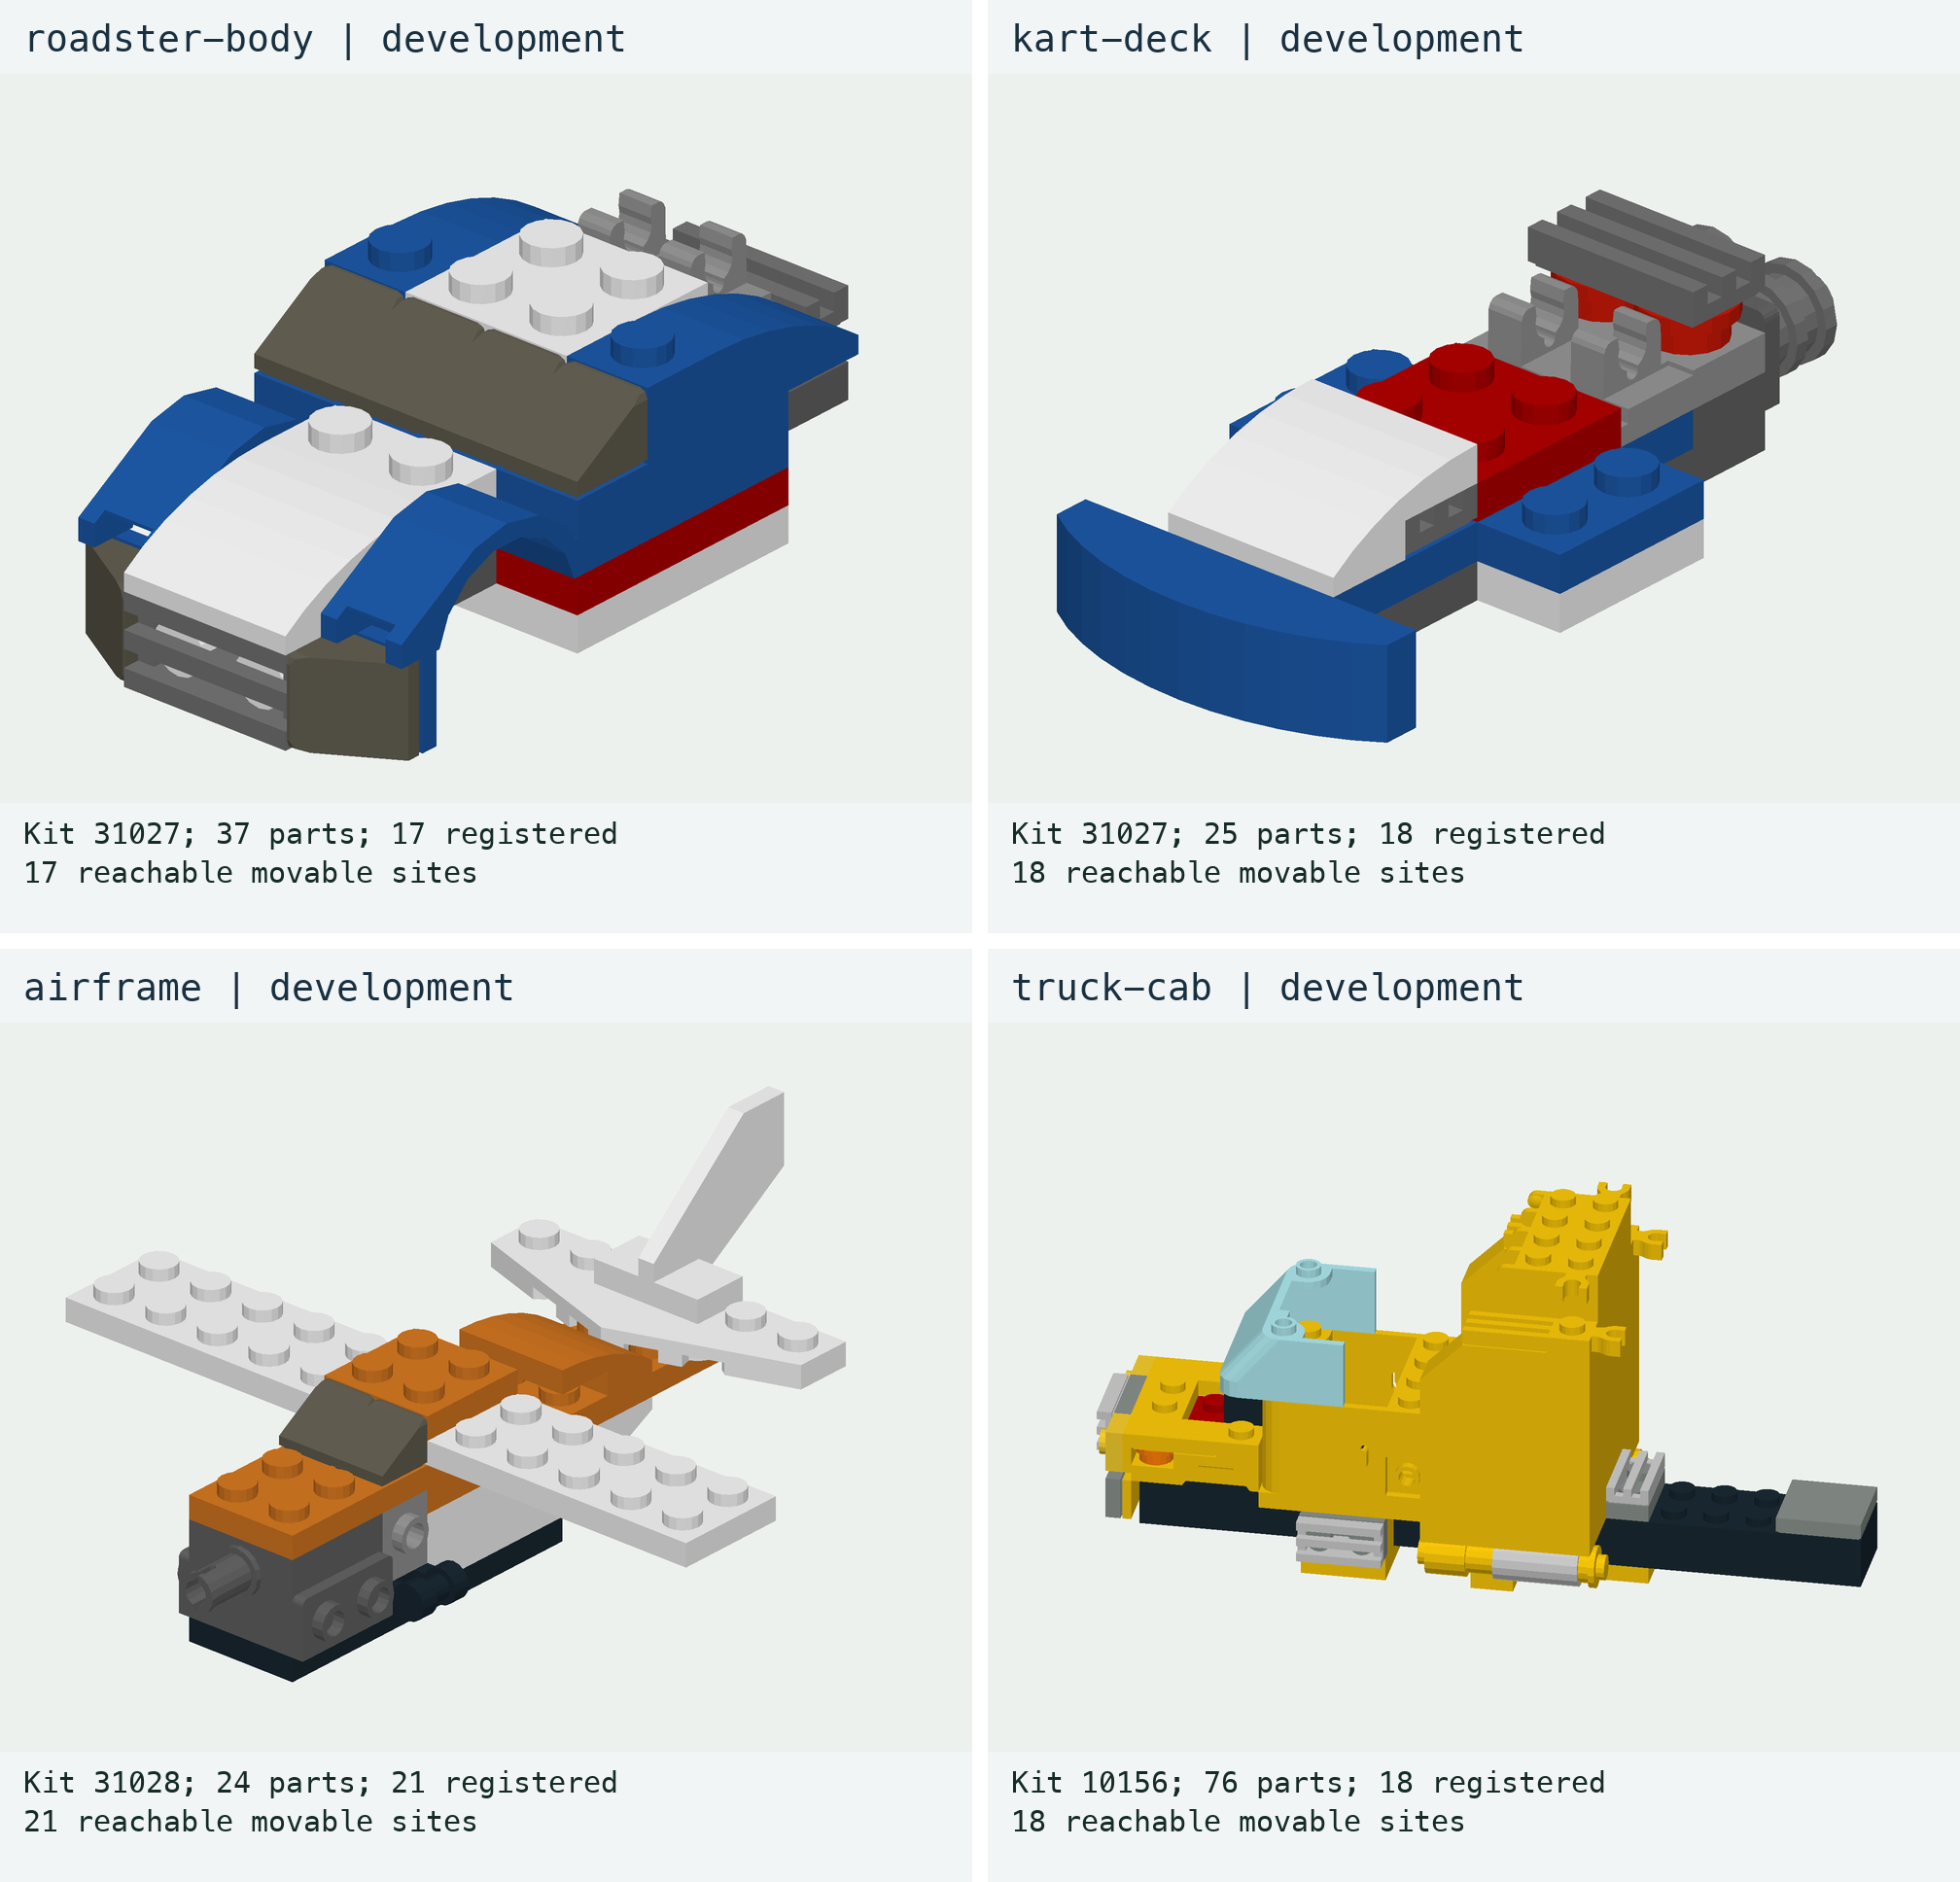
\includegraphics[width=.96\textwidth,height=.85\textheight,keepaspectratio]{figures/source-gallery-1.png}
\end{center}
\clearpage
\section*{Original-source gallery: assemblies 5--8}
\begin{center}
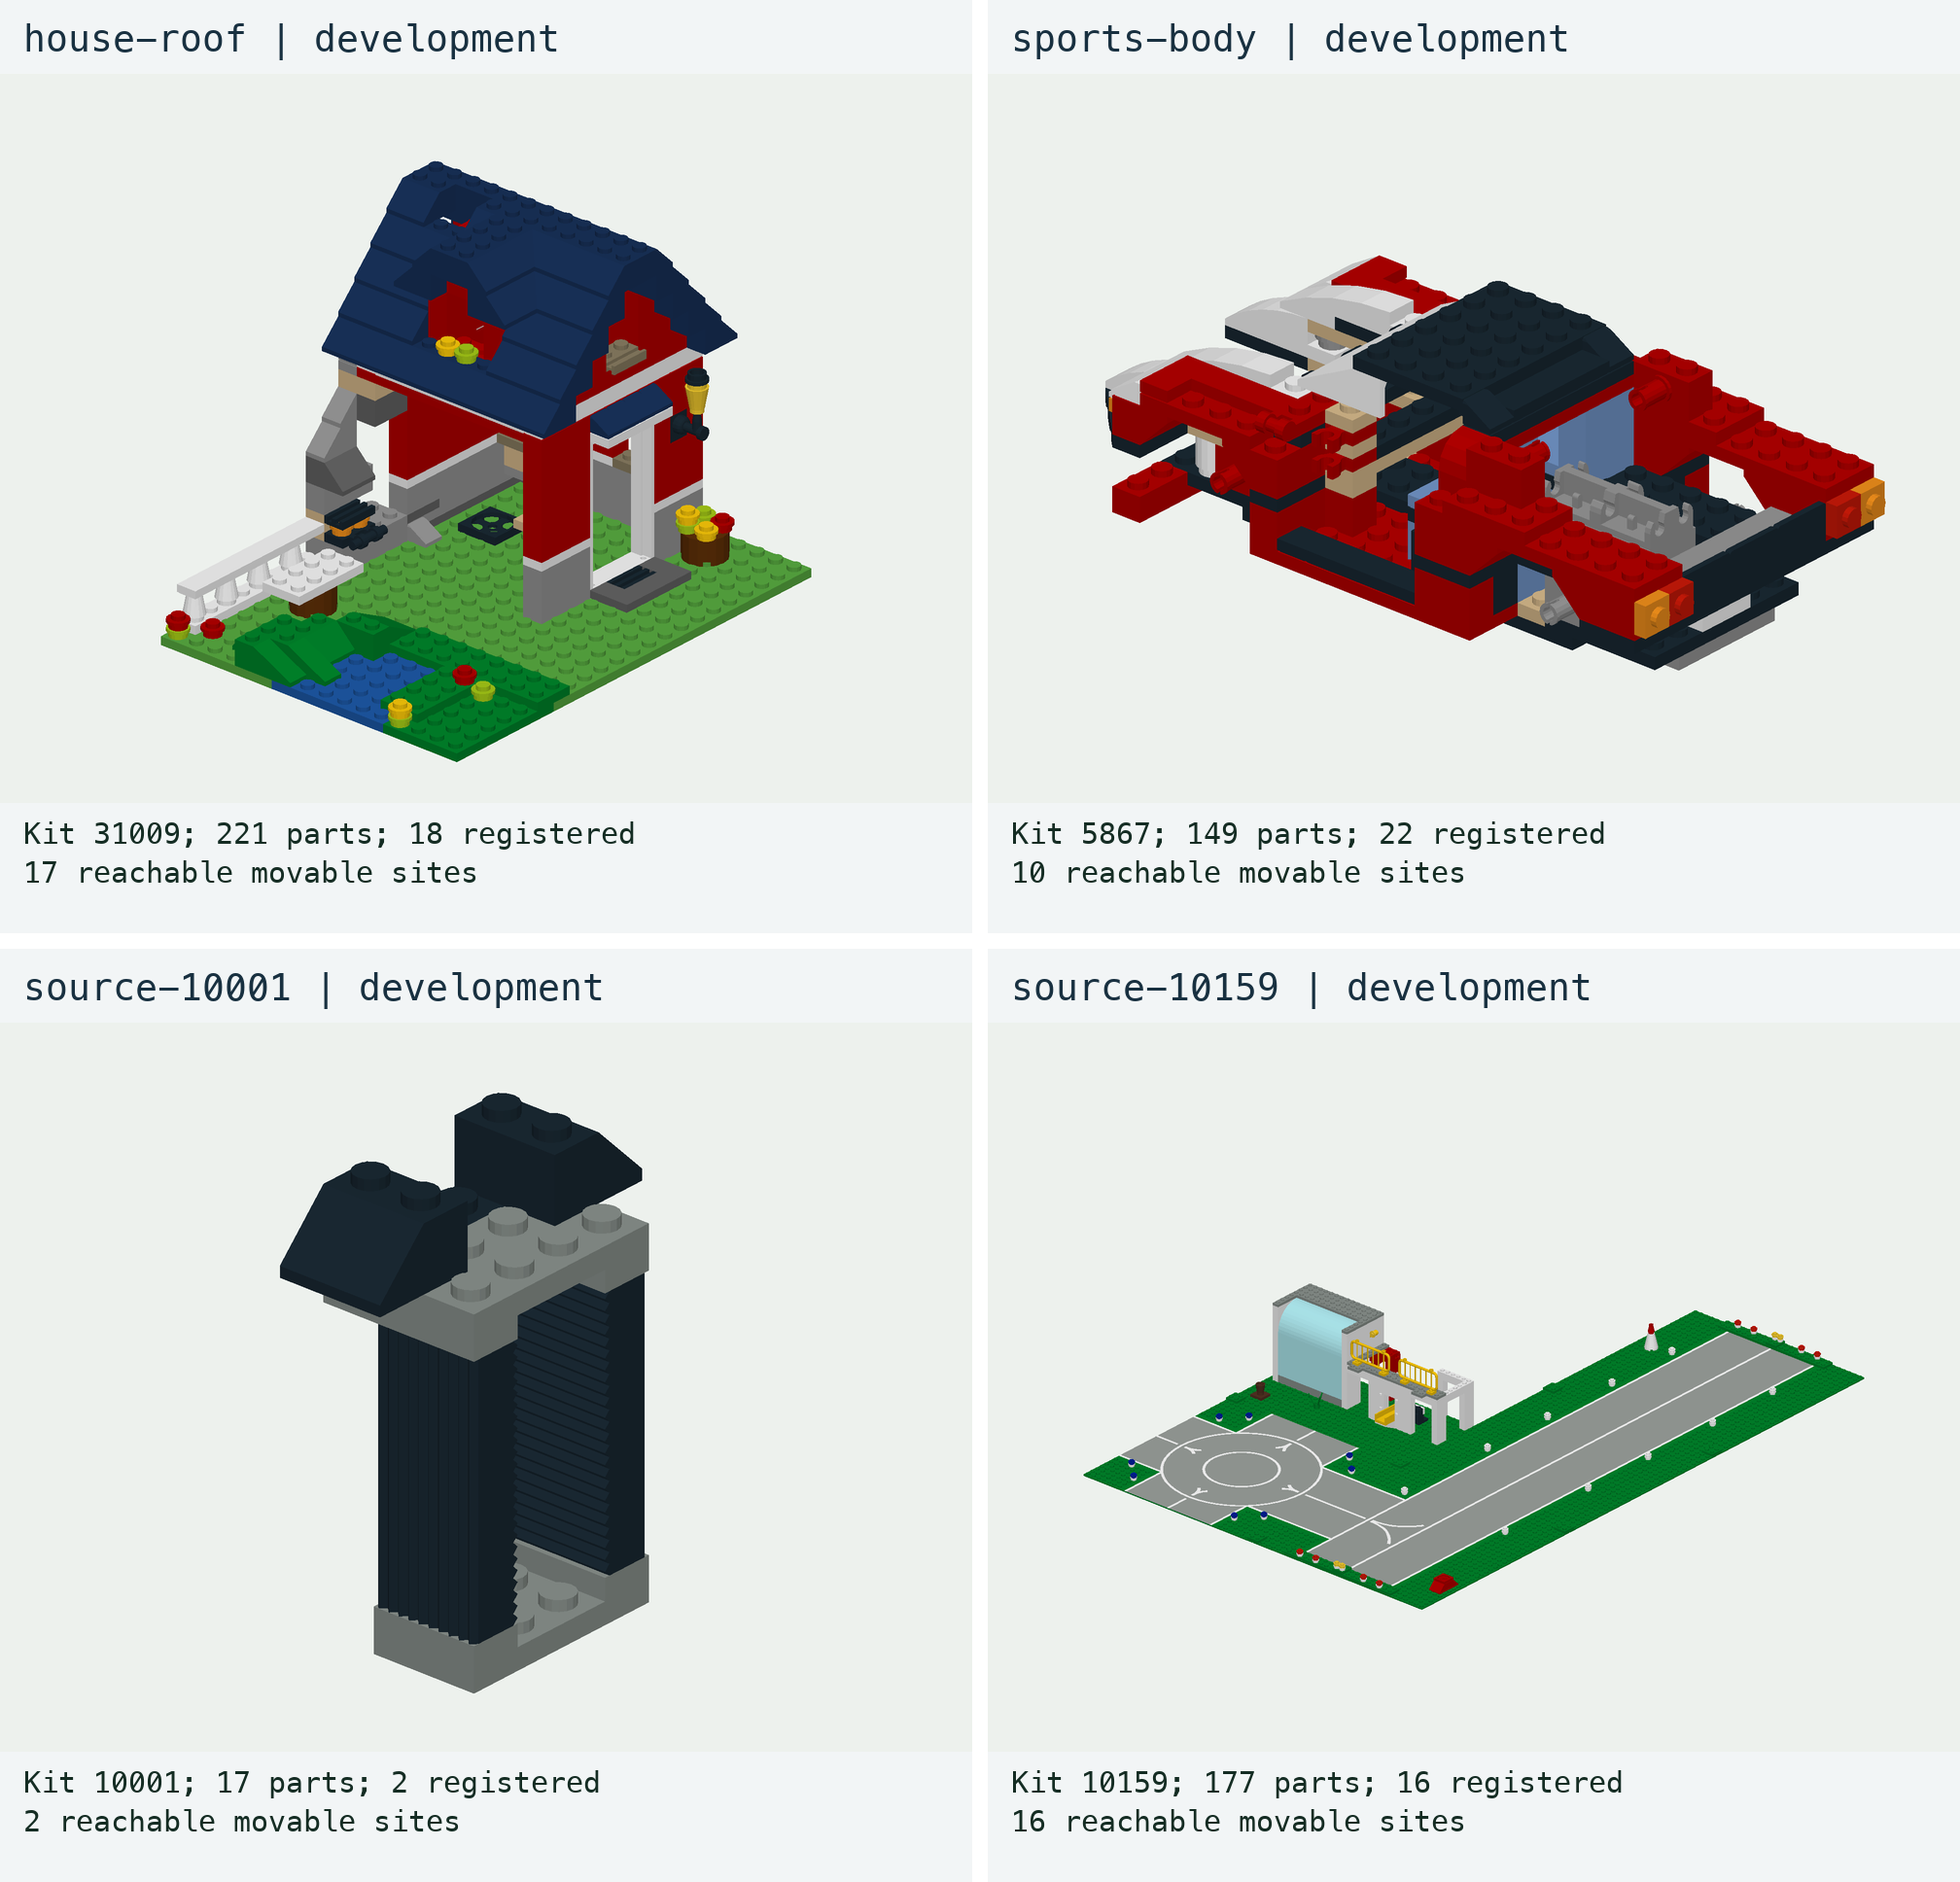
\includegraphics[width=.96\textwidth,height=.85\textheight,keepaspectratio]{figures/source-gallery-2.png}
\end{center}
\clearpage
\section*{Original-source gallery: assemblies 9--12}
\begin{center}
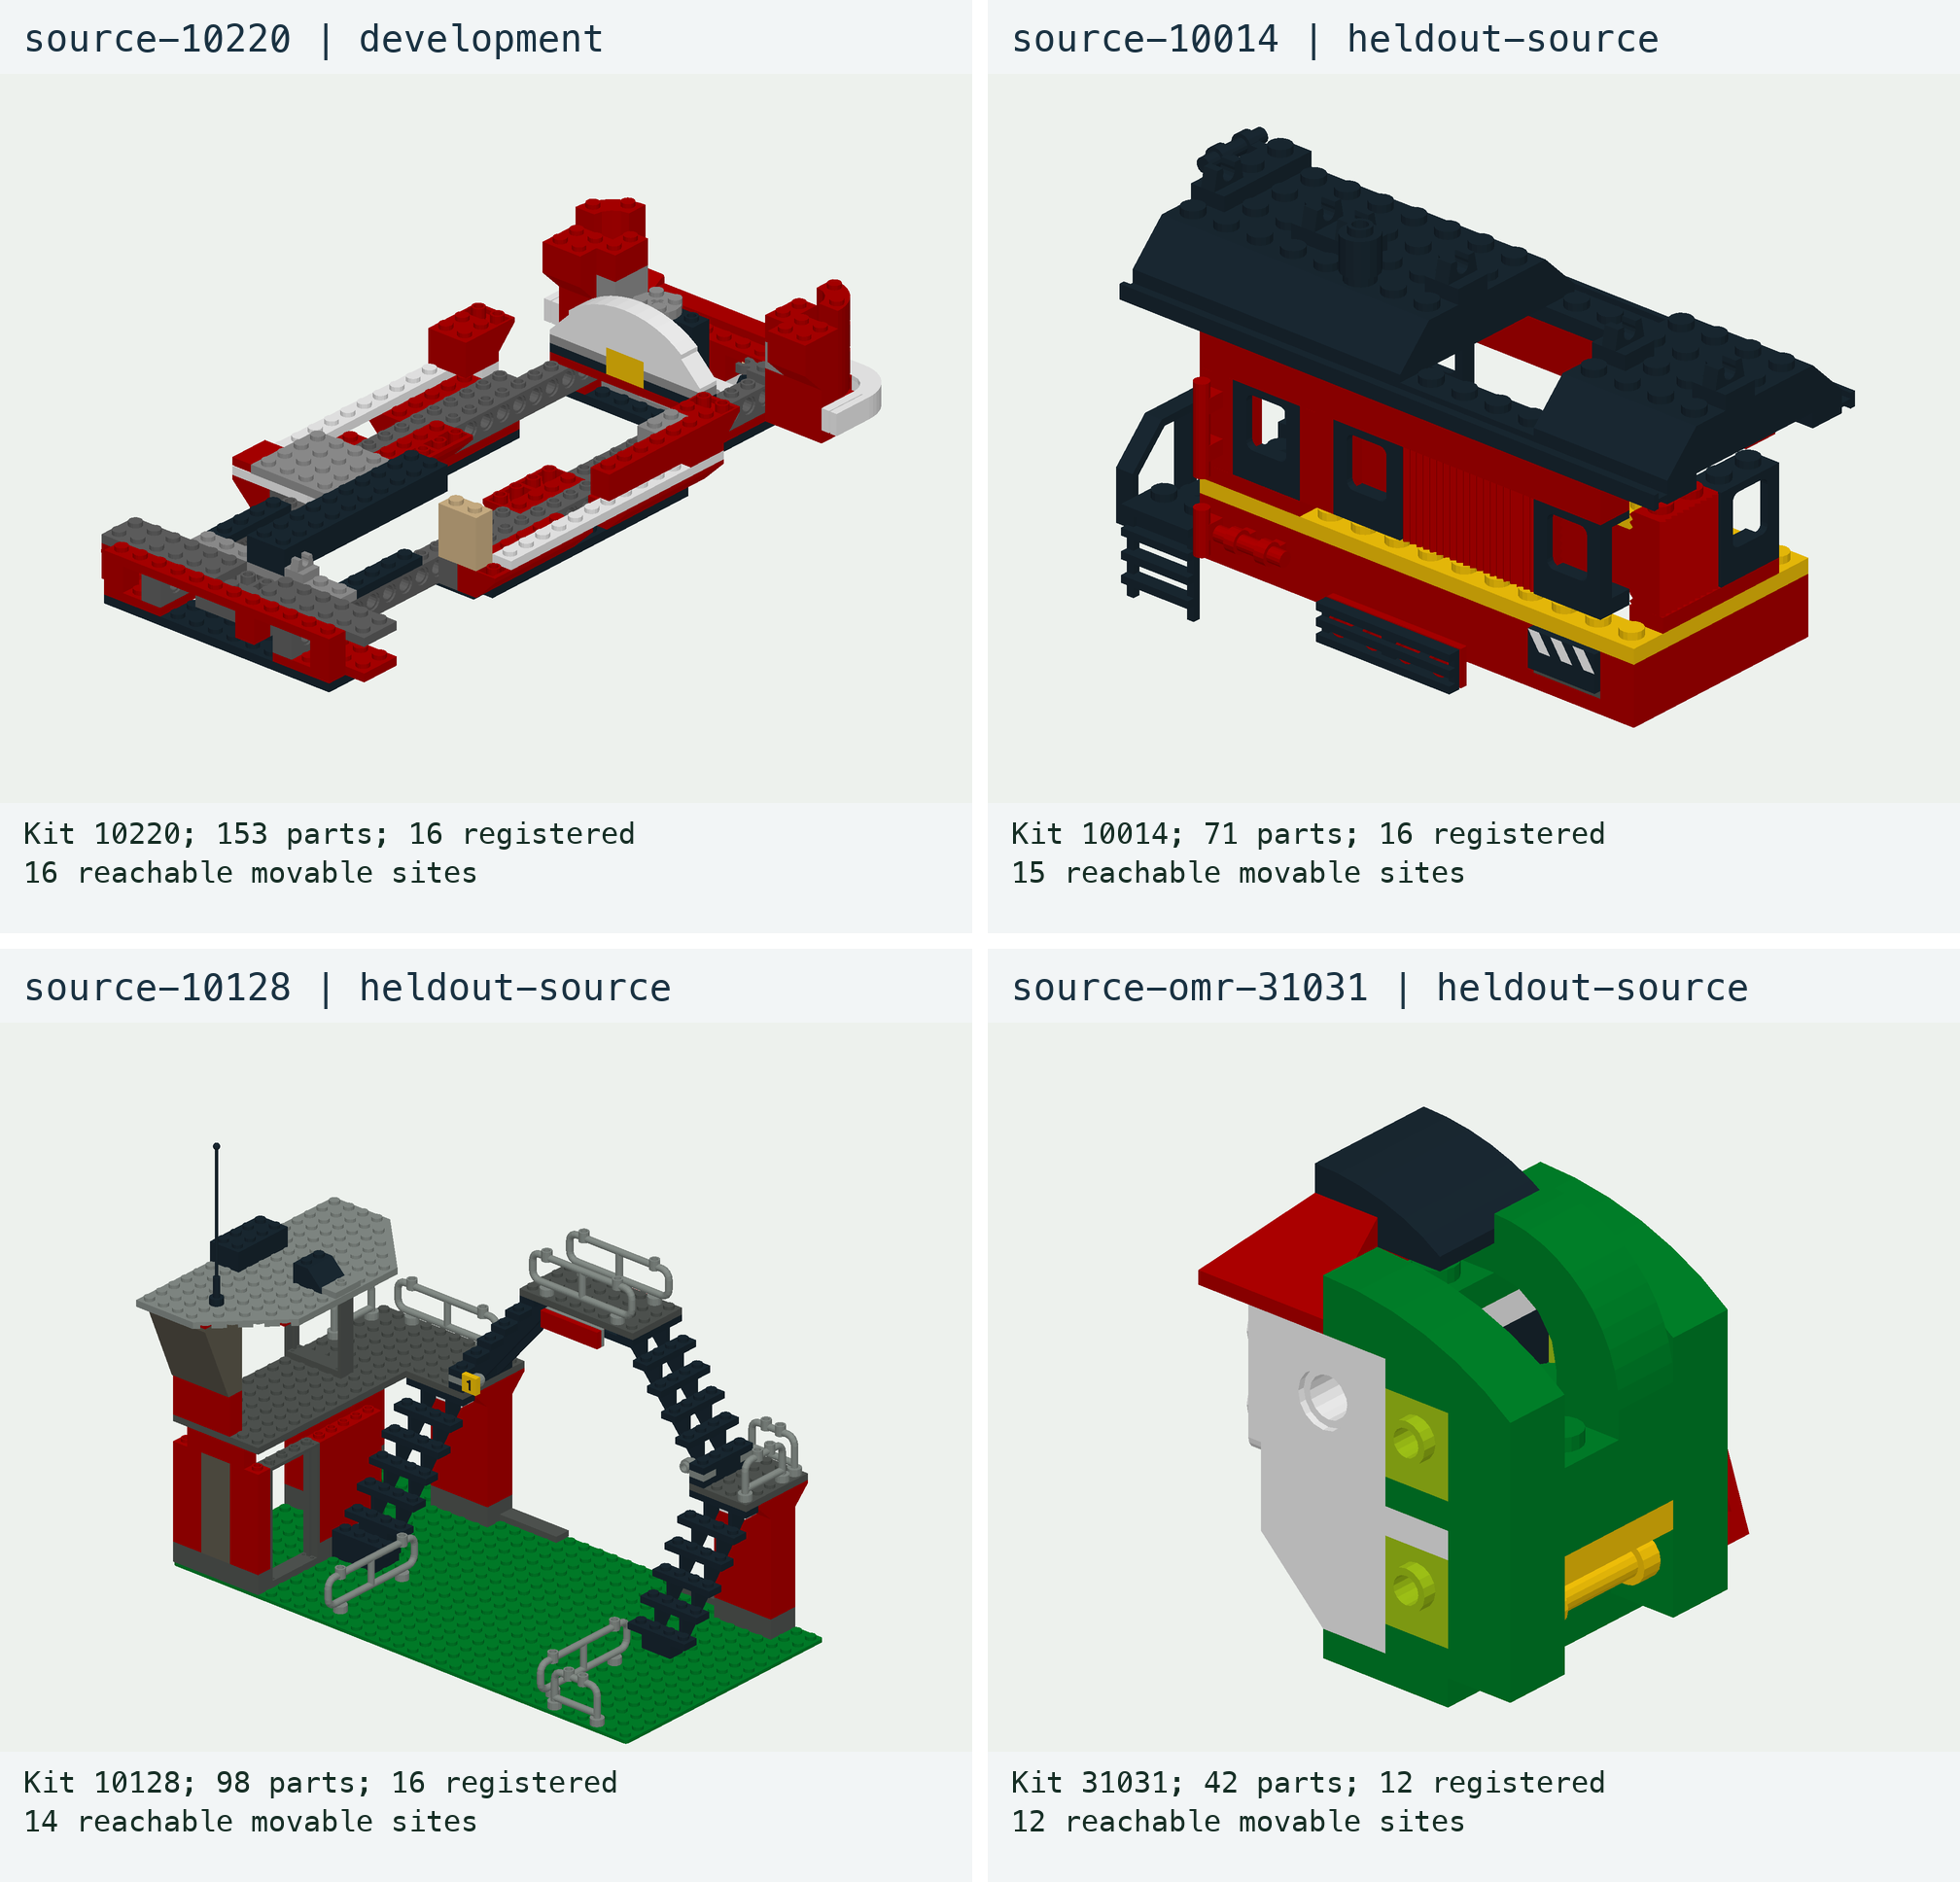
\includegraphics[width=.96\textwidth,height=.85\textheight,keepaspectratio]{figures/source-gallery-3.png}
\end{center}
\clearpage
\section*{Original-source gallery: assemblies 13--16}
\begin{center}
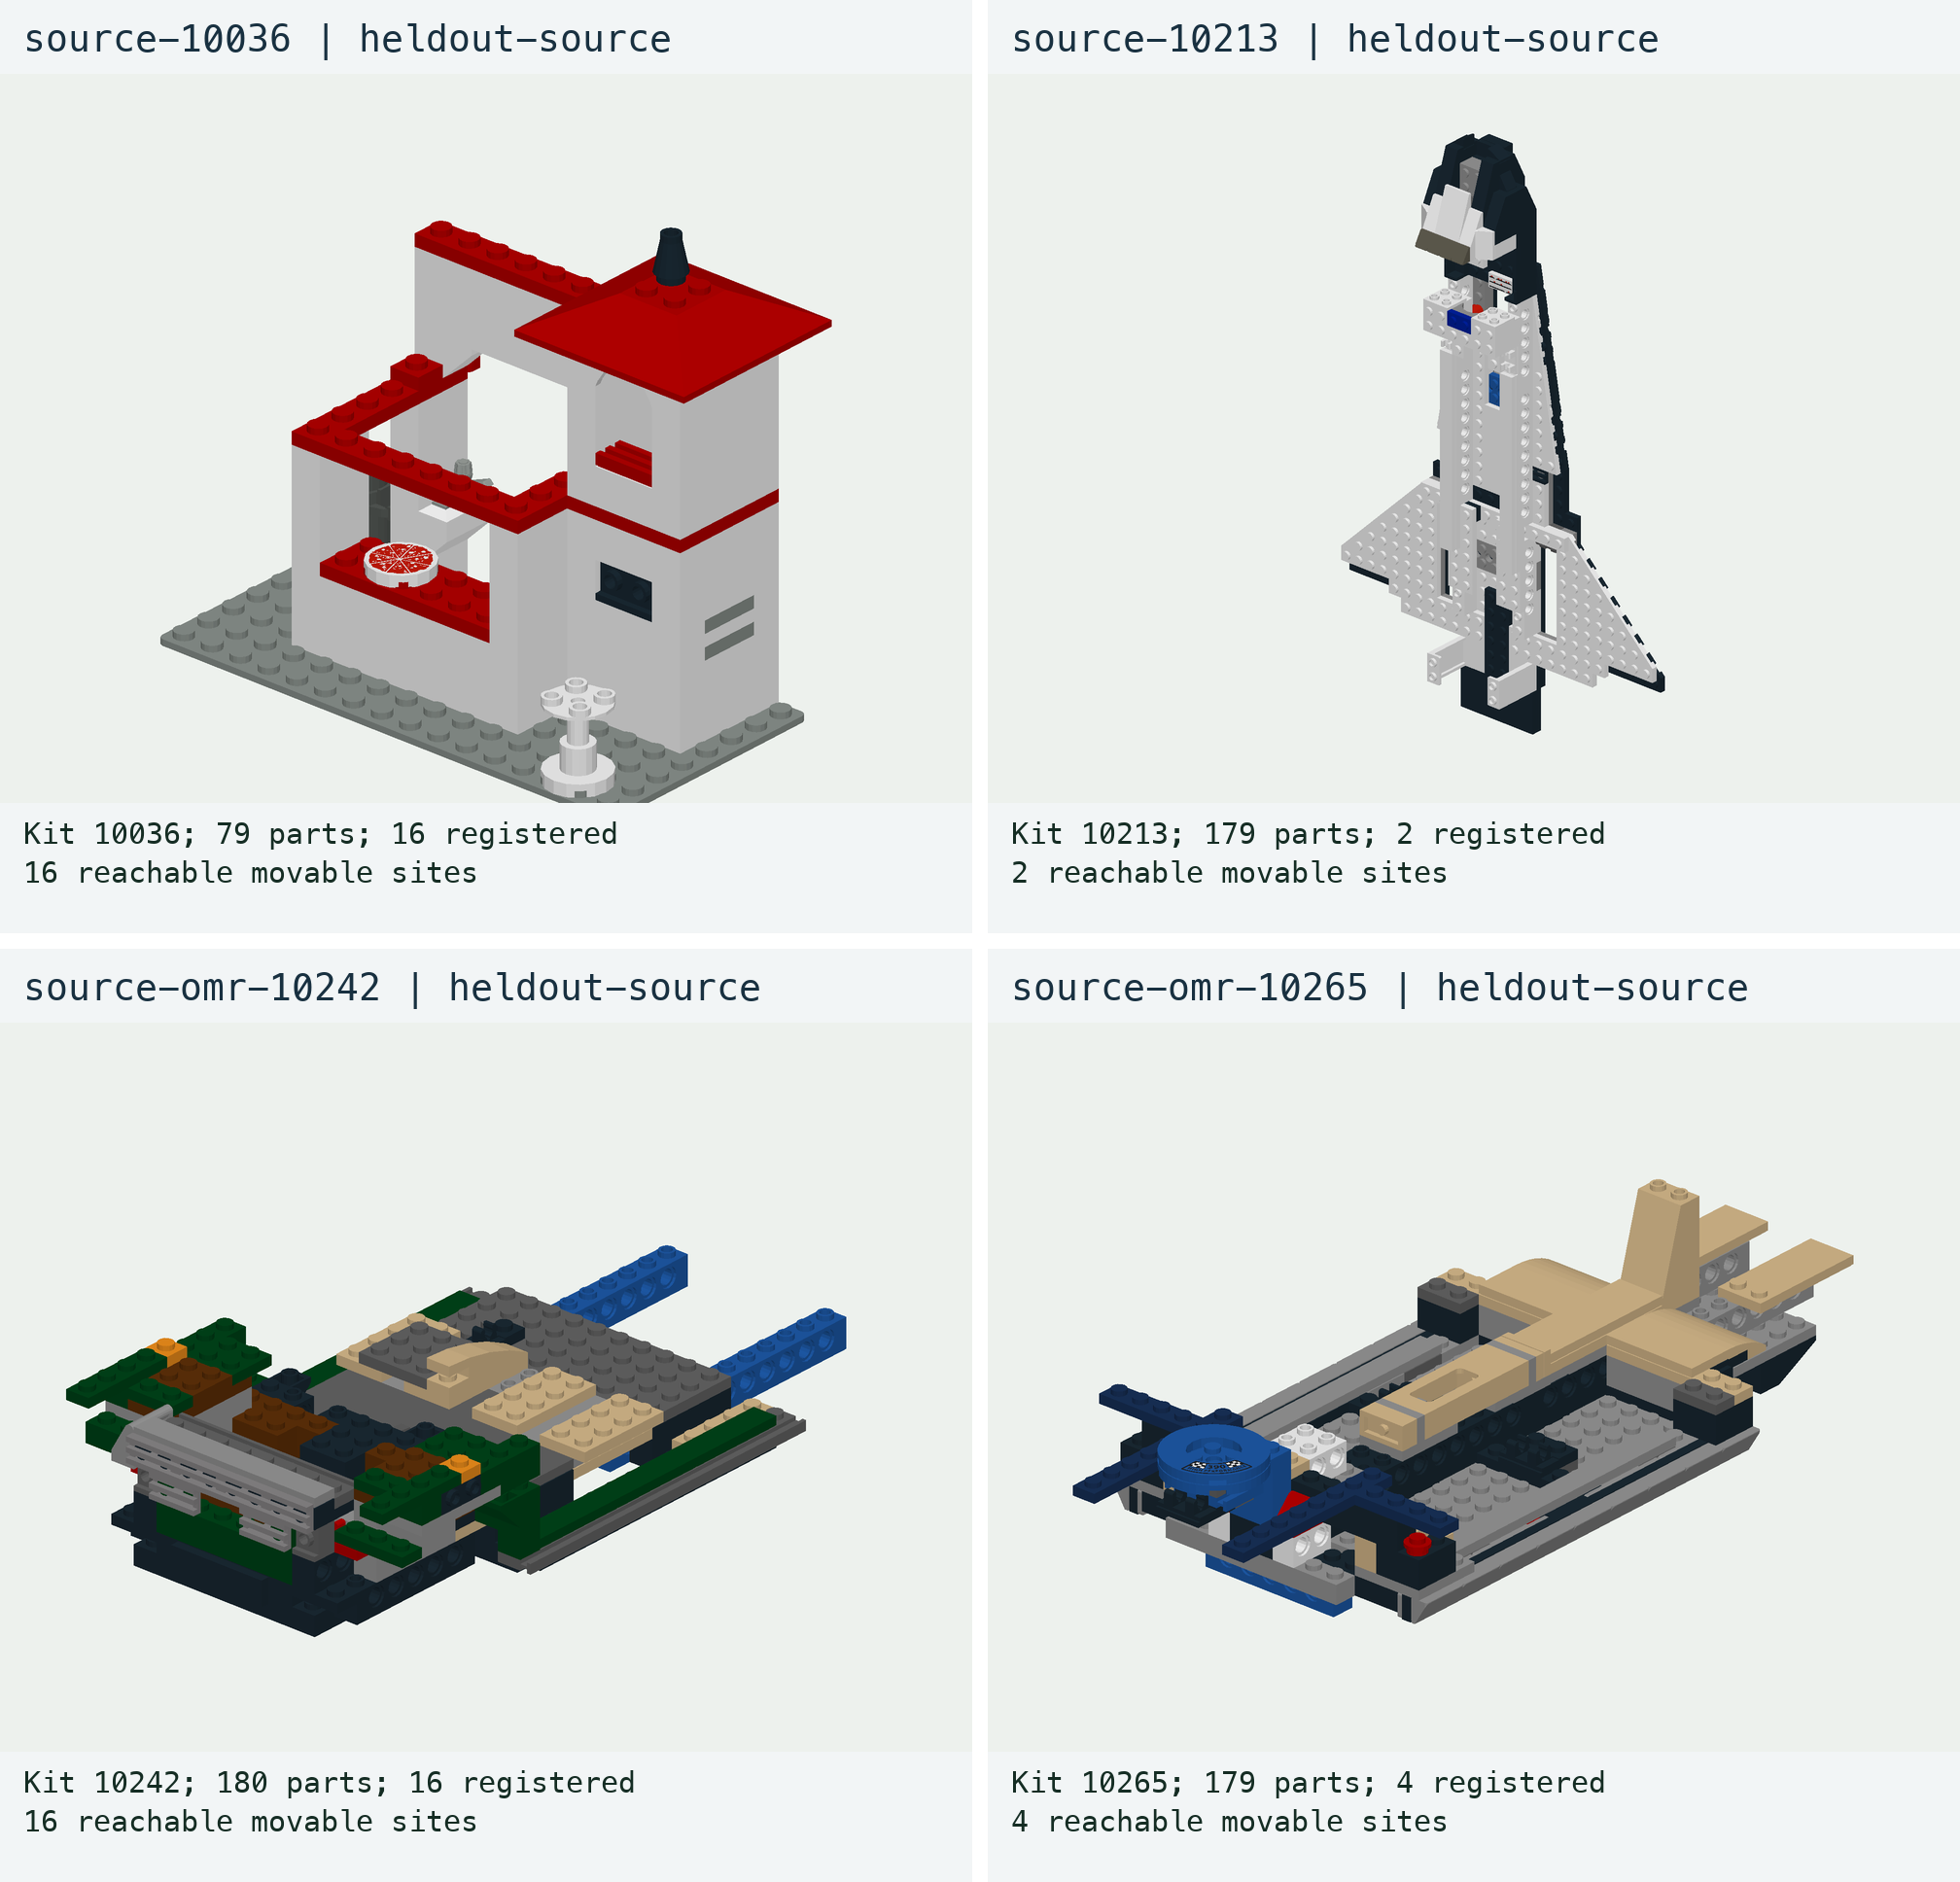
\includegraphics[width=.96\textwidth,height=.85\textheight,keepaspectratio]{figures/source-gallery-4.png}
\end{center}
\clearpage
\section*{Original-source gallery: assemblies 17--20}
\begin{center}
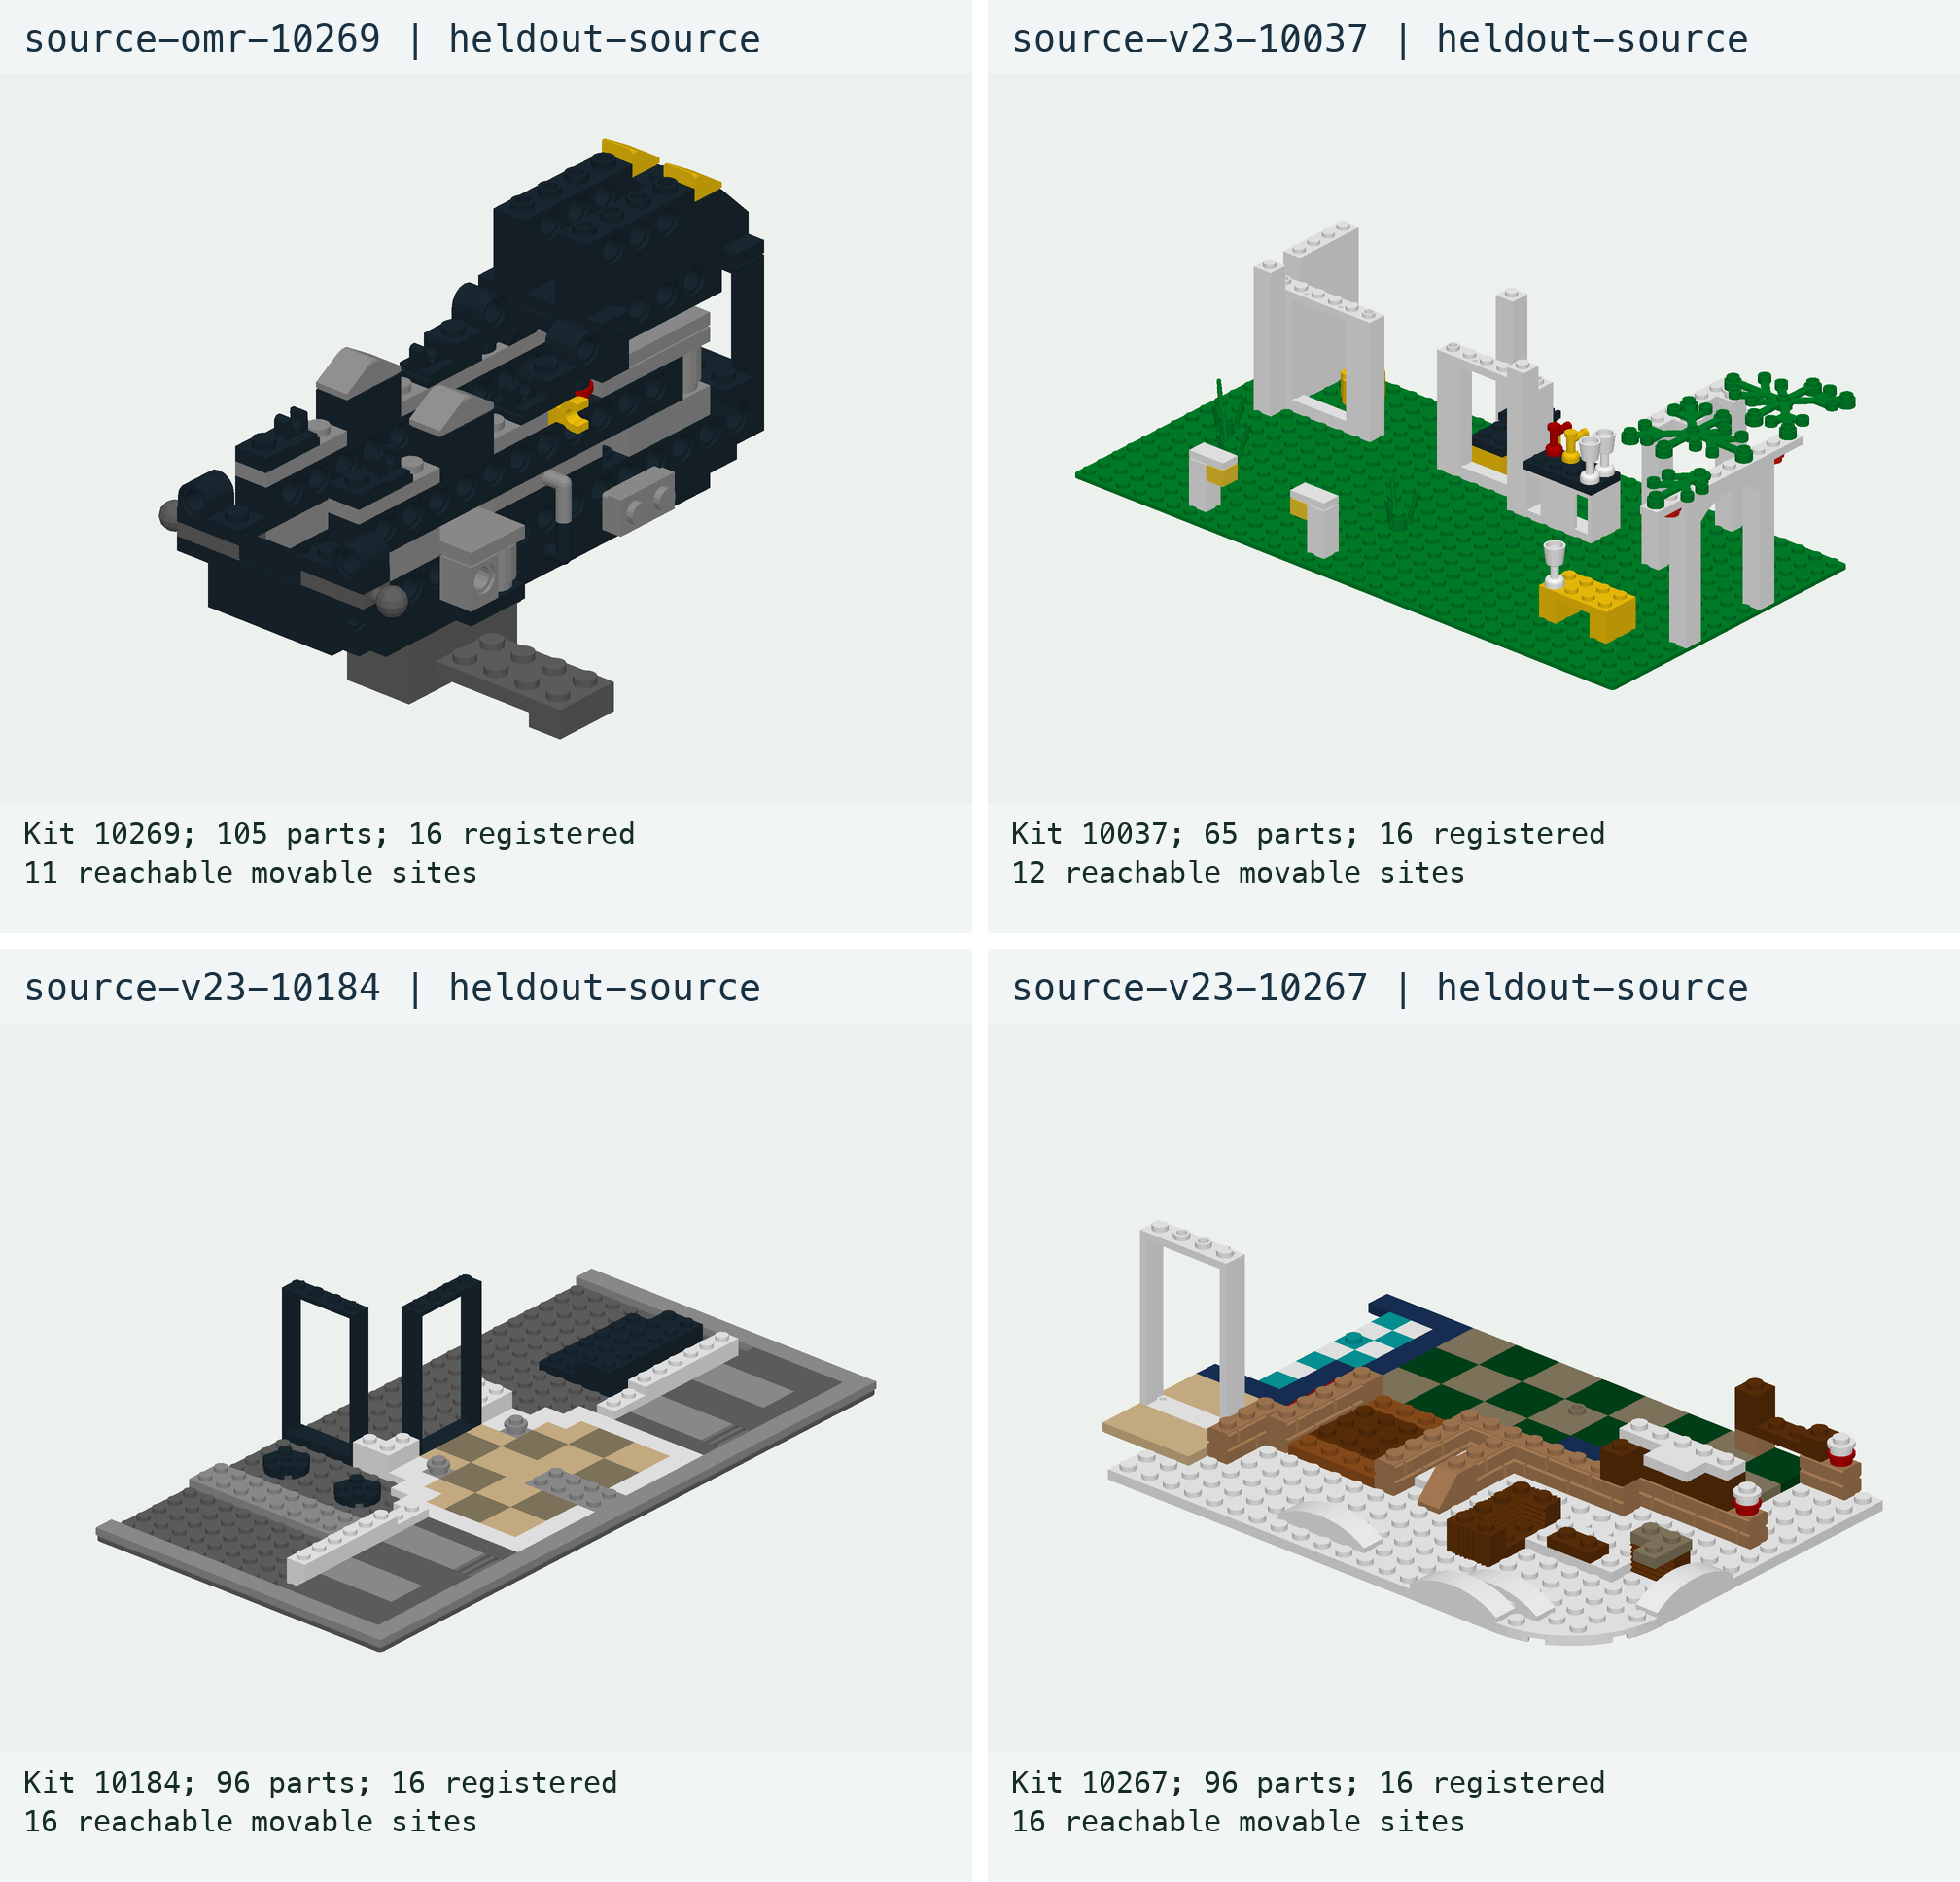
\includegraphics[width=.96\textwidth,height=.85\textheight,keepaspectratio]{figures/source-gallery-5.png}
\end{center}
\clearpage
\section*{Original-source gallery: assemblies 21--24}
\begin{center}
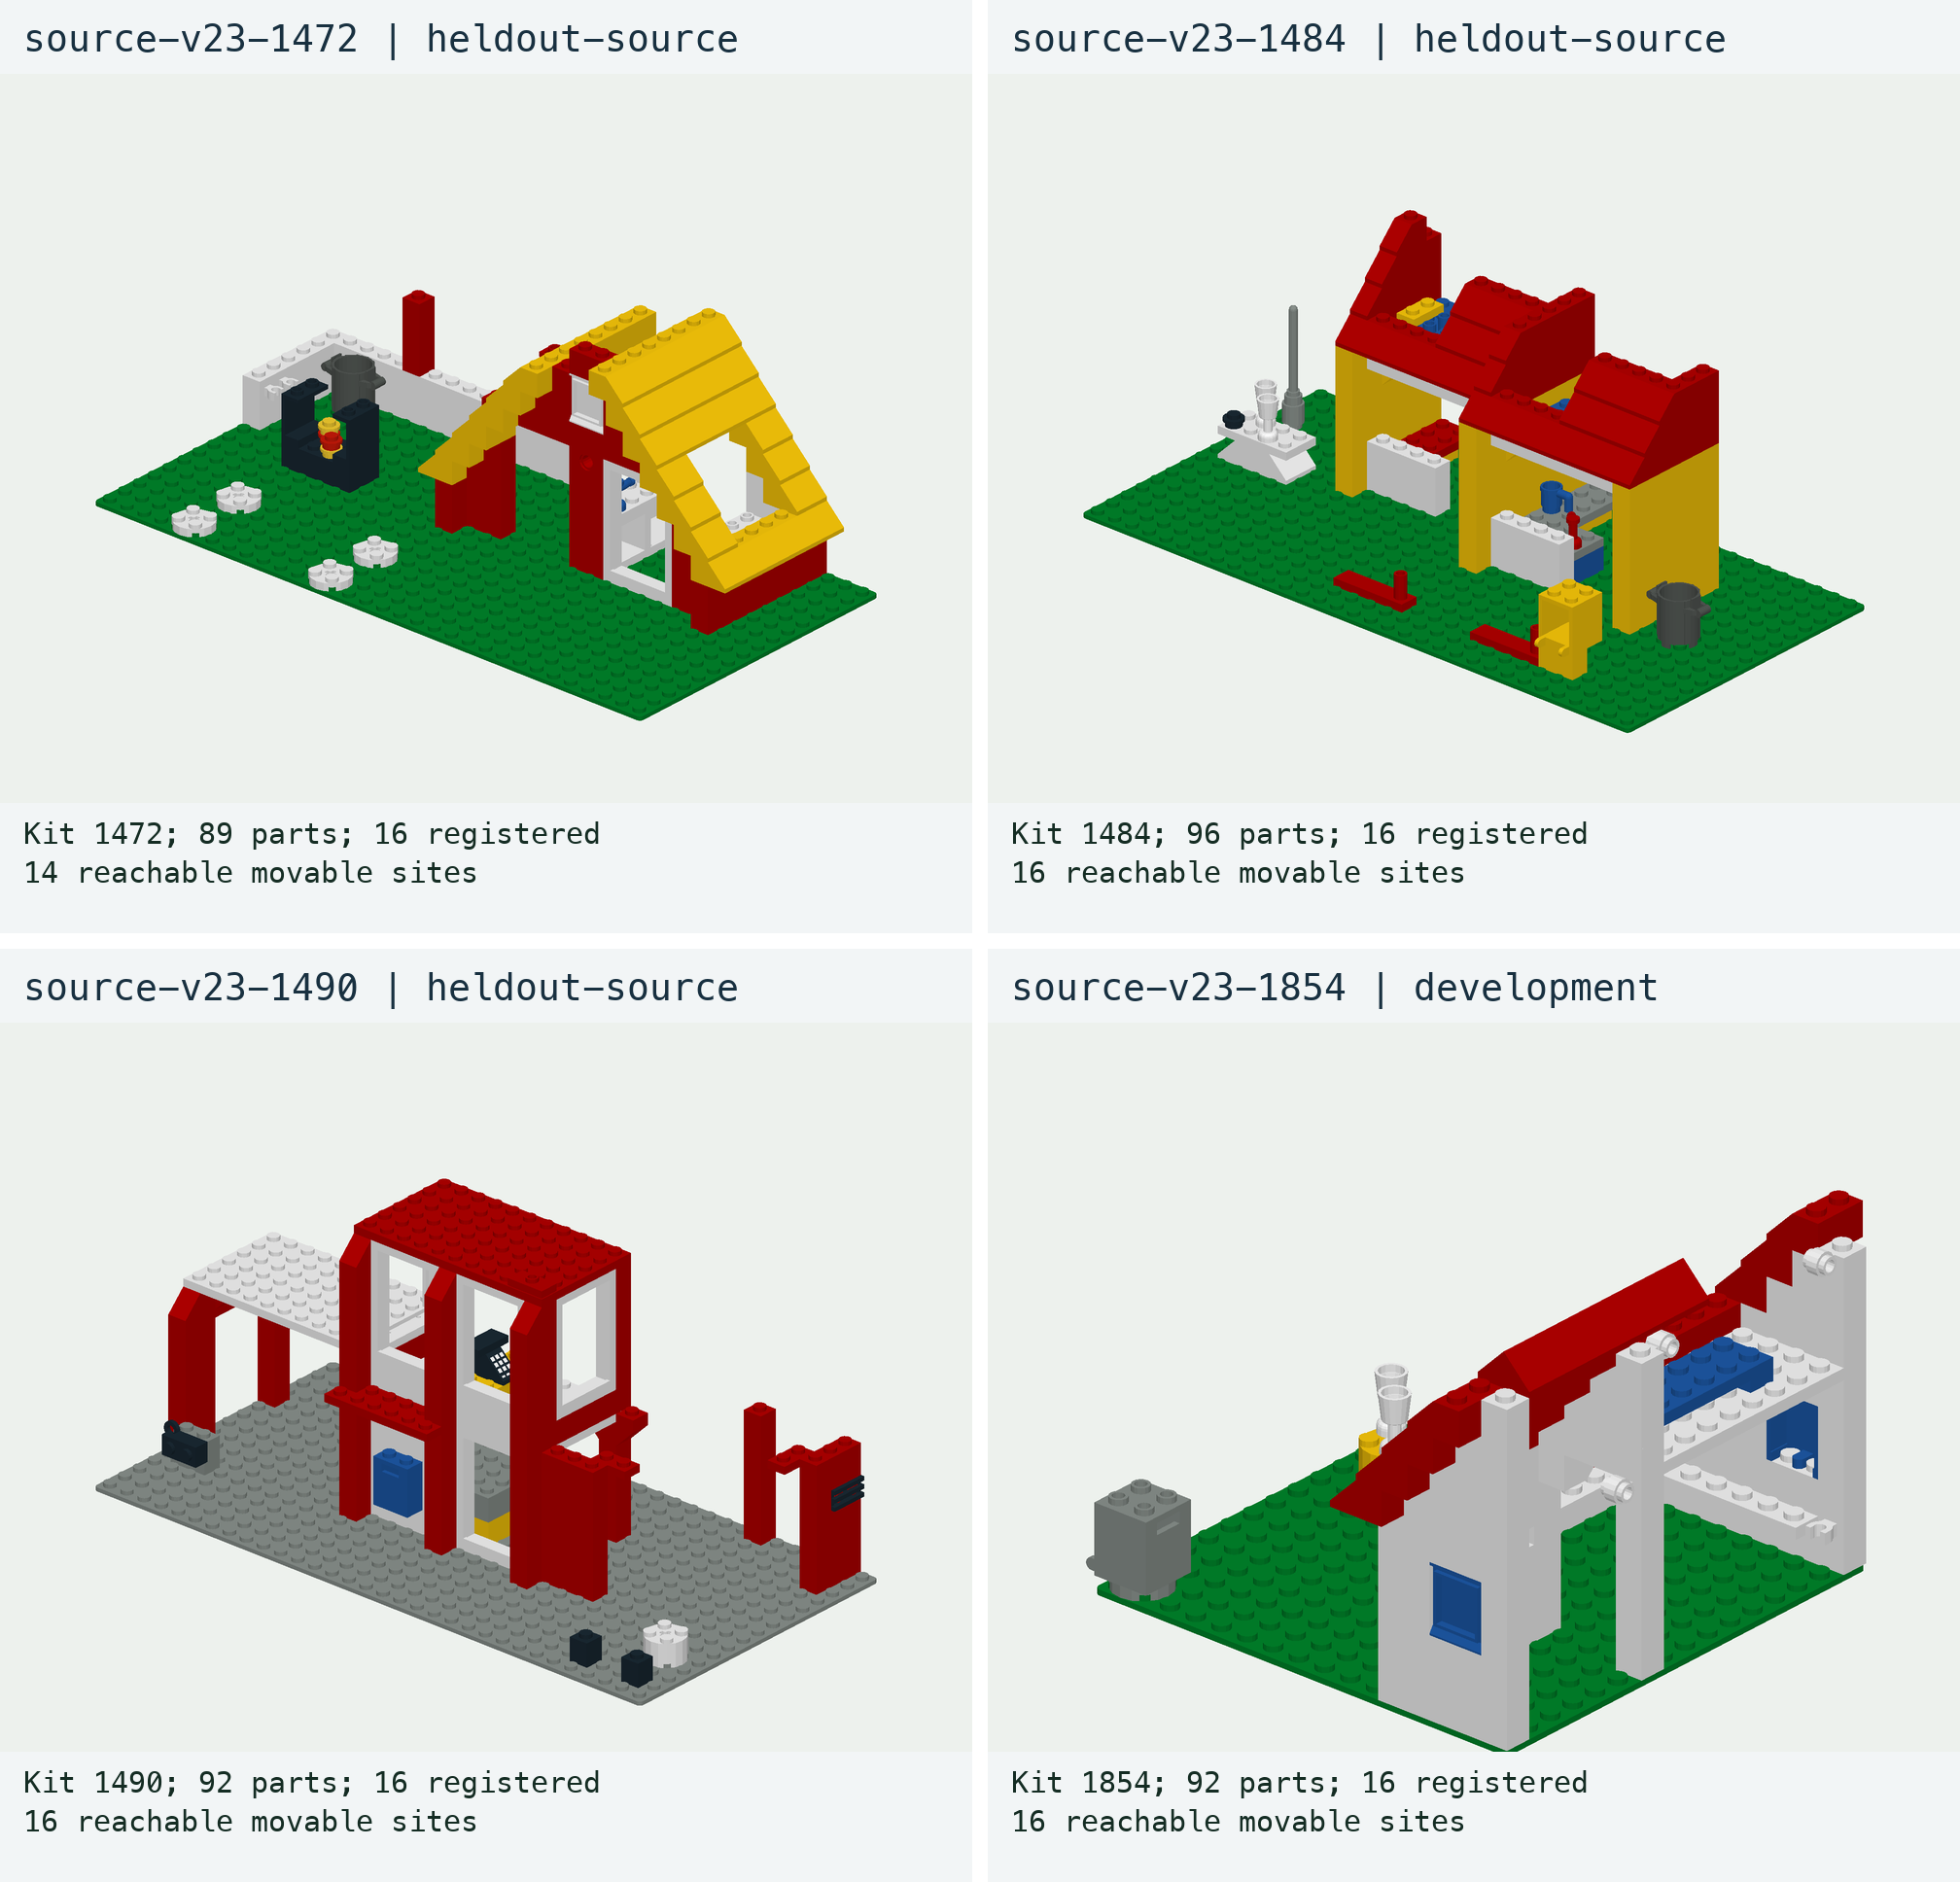
\includegraphics[width=.96\textwidth,height=.85\textheight,keepaspectratio]{figures/source-gallery-6.png}
\end{center}
\clearpage
\section*{Original-source gallery: assemblies 25--28}
\begin{center}
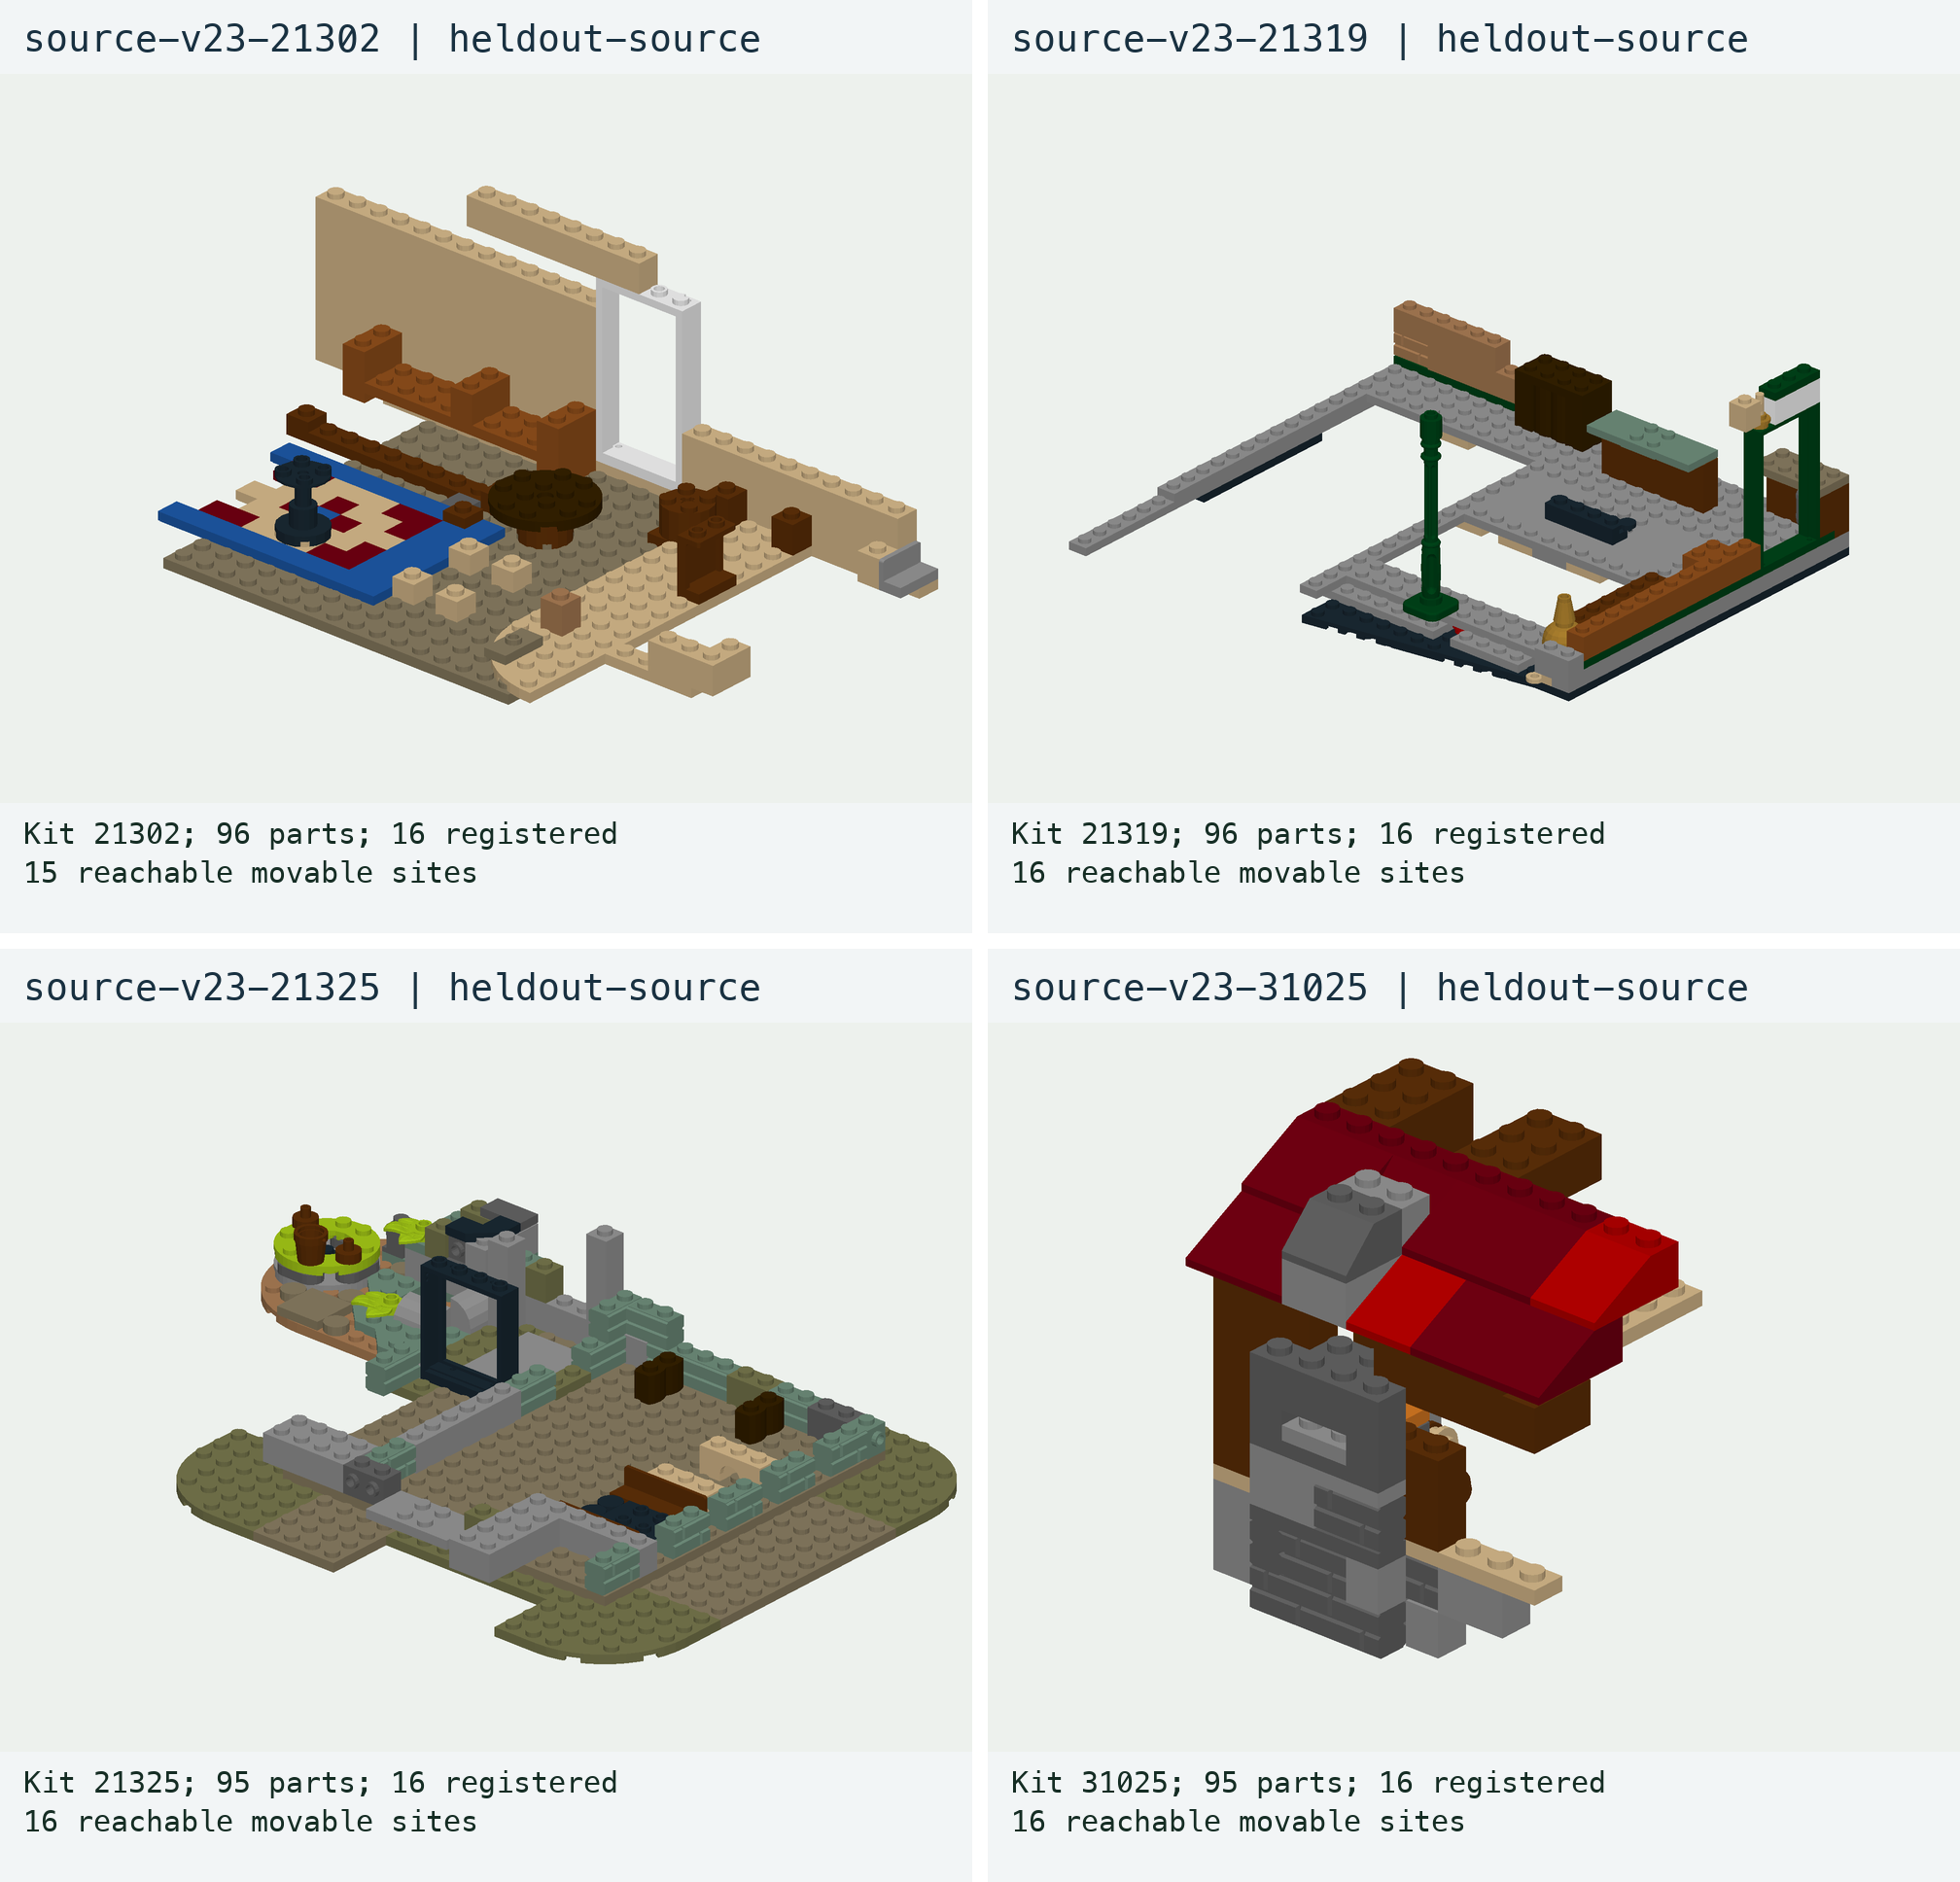
\includegraphics[width=.96\textwidth,height=.85\textheight,keepaspectratio]{figures/source-gallery-7.png}
\end{center}
\clearpage
\section*{Original-source gallery: assemblies 29--32}
\begin{center}
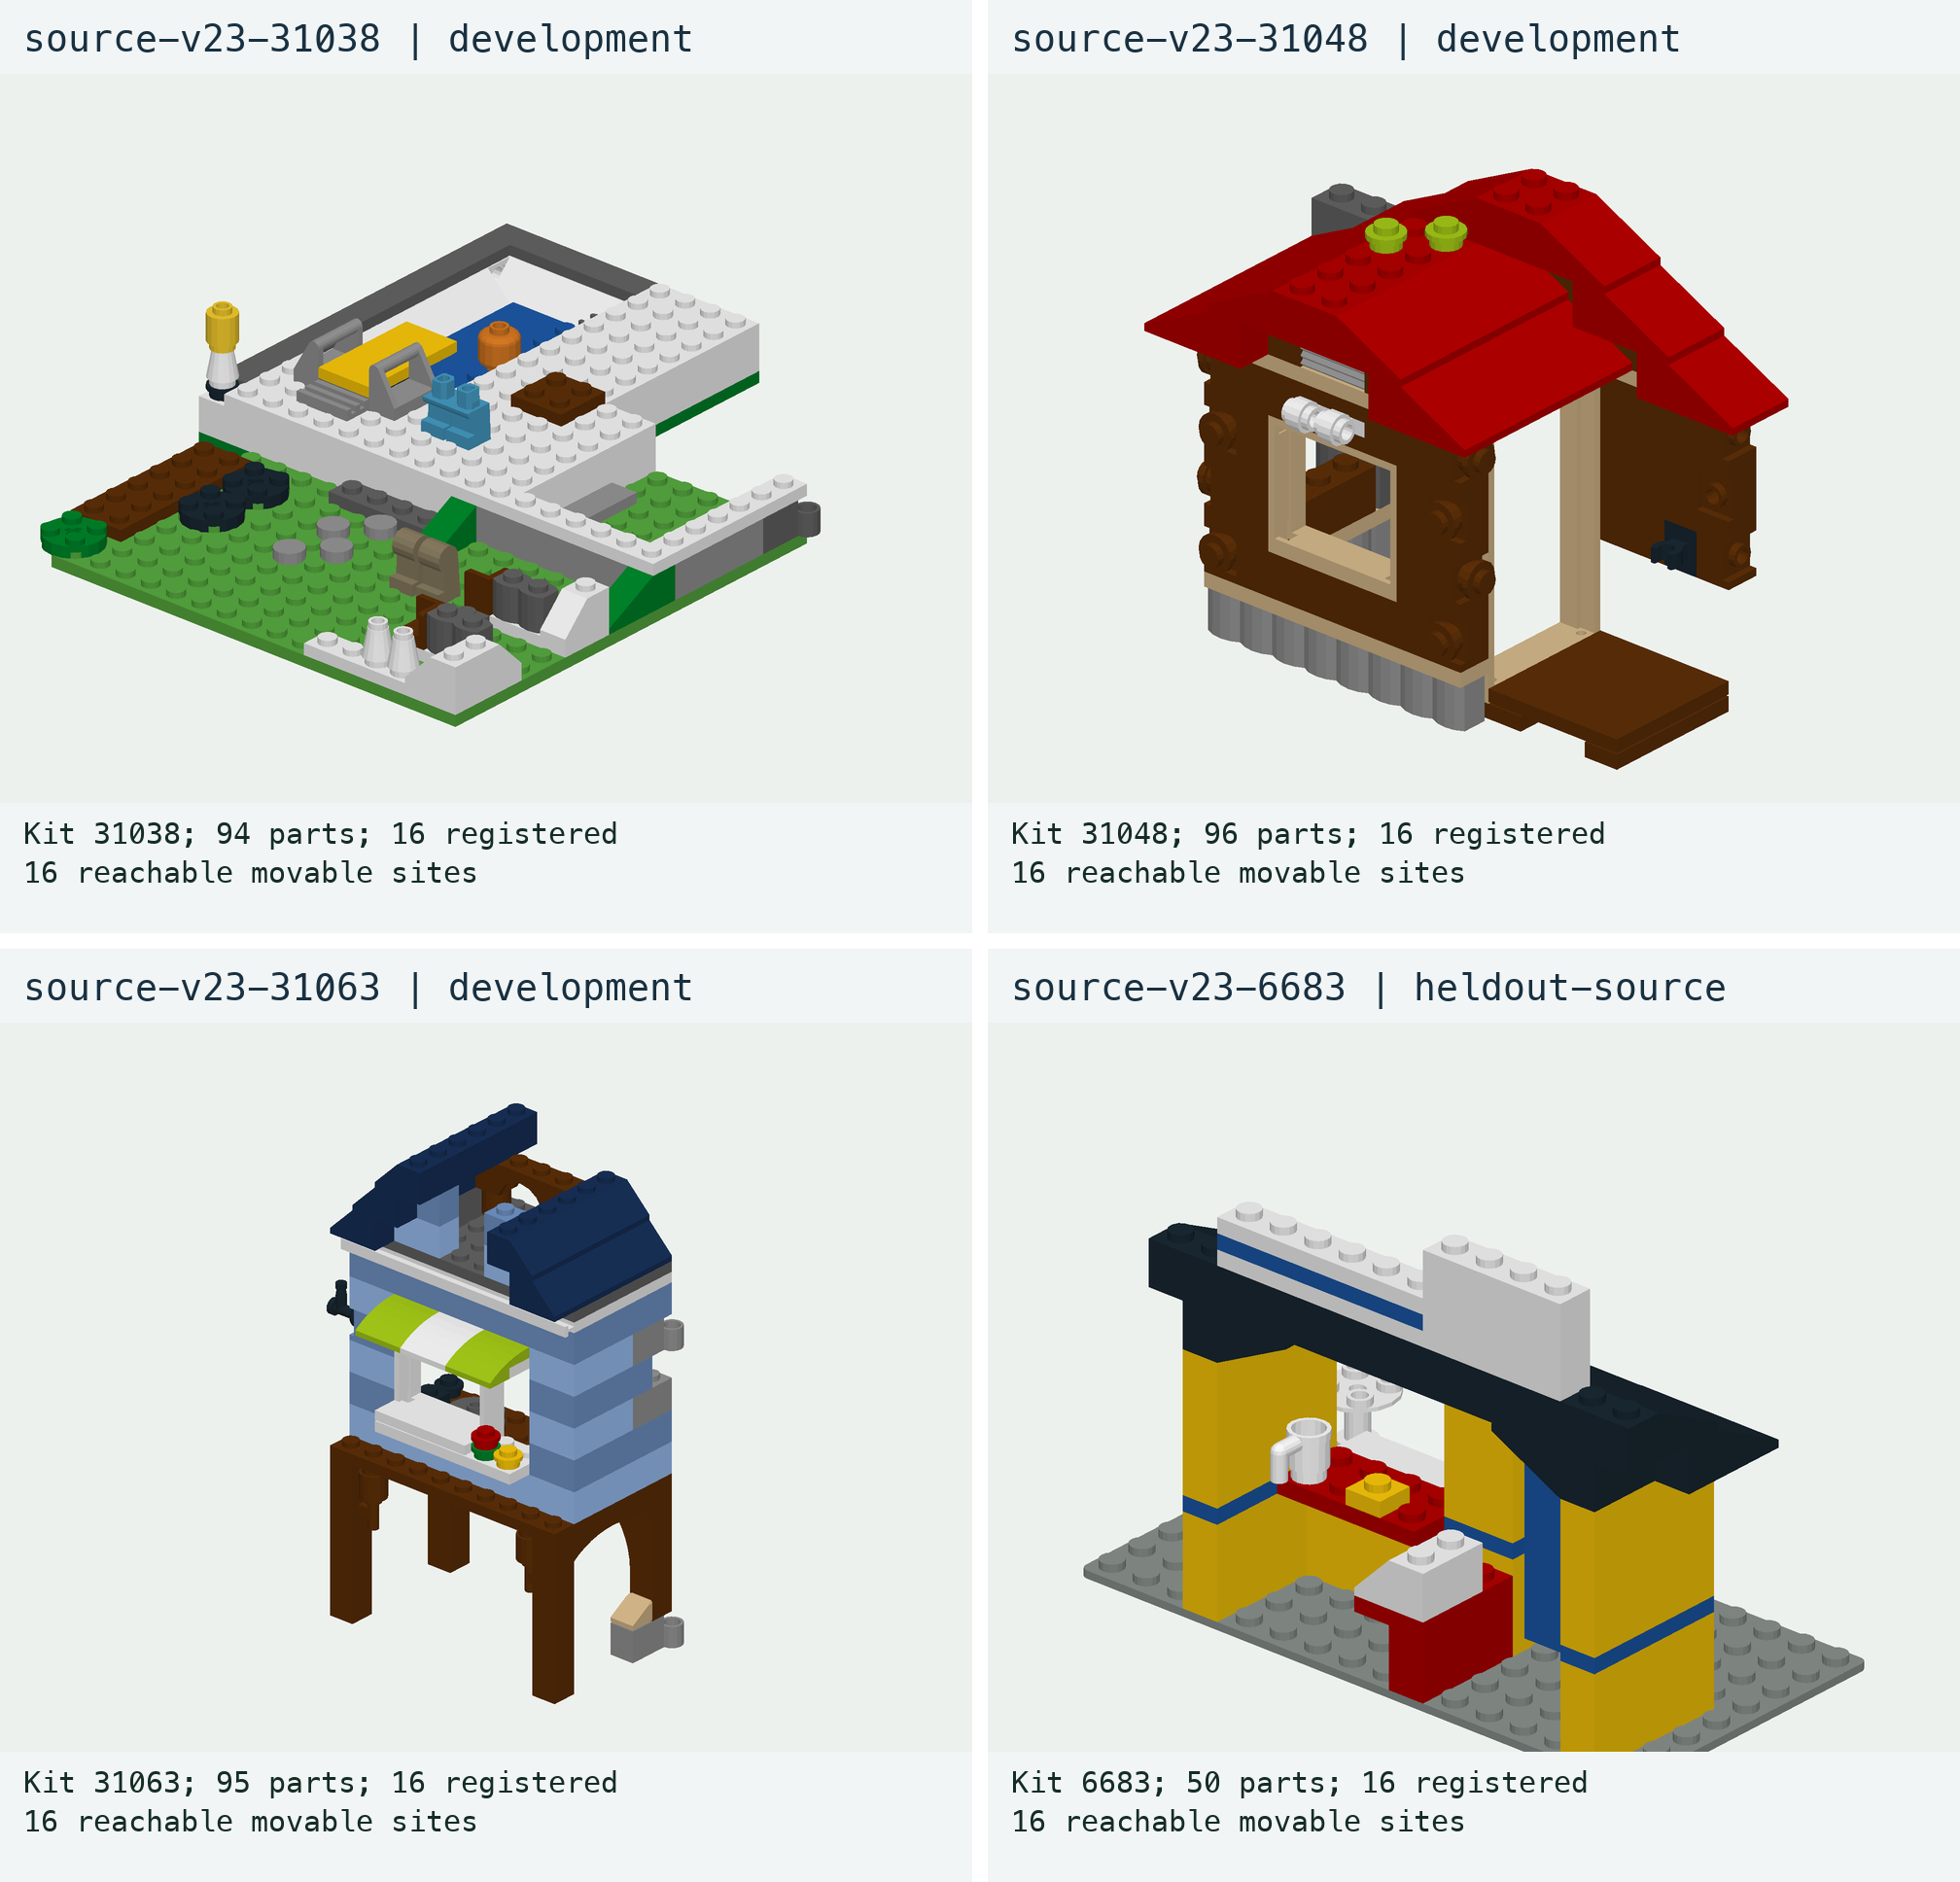
\includegraphics[width=.96\textwidth,height=.85\textheight,keepaspectratio]{figures/source-gallery-8.png}
\end{center}
\clearpage
\section*{Original-source gallery: assemblies 33--36}
\begin{center}
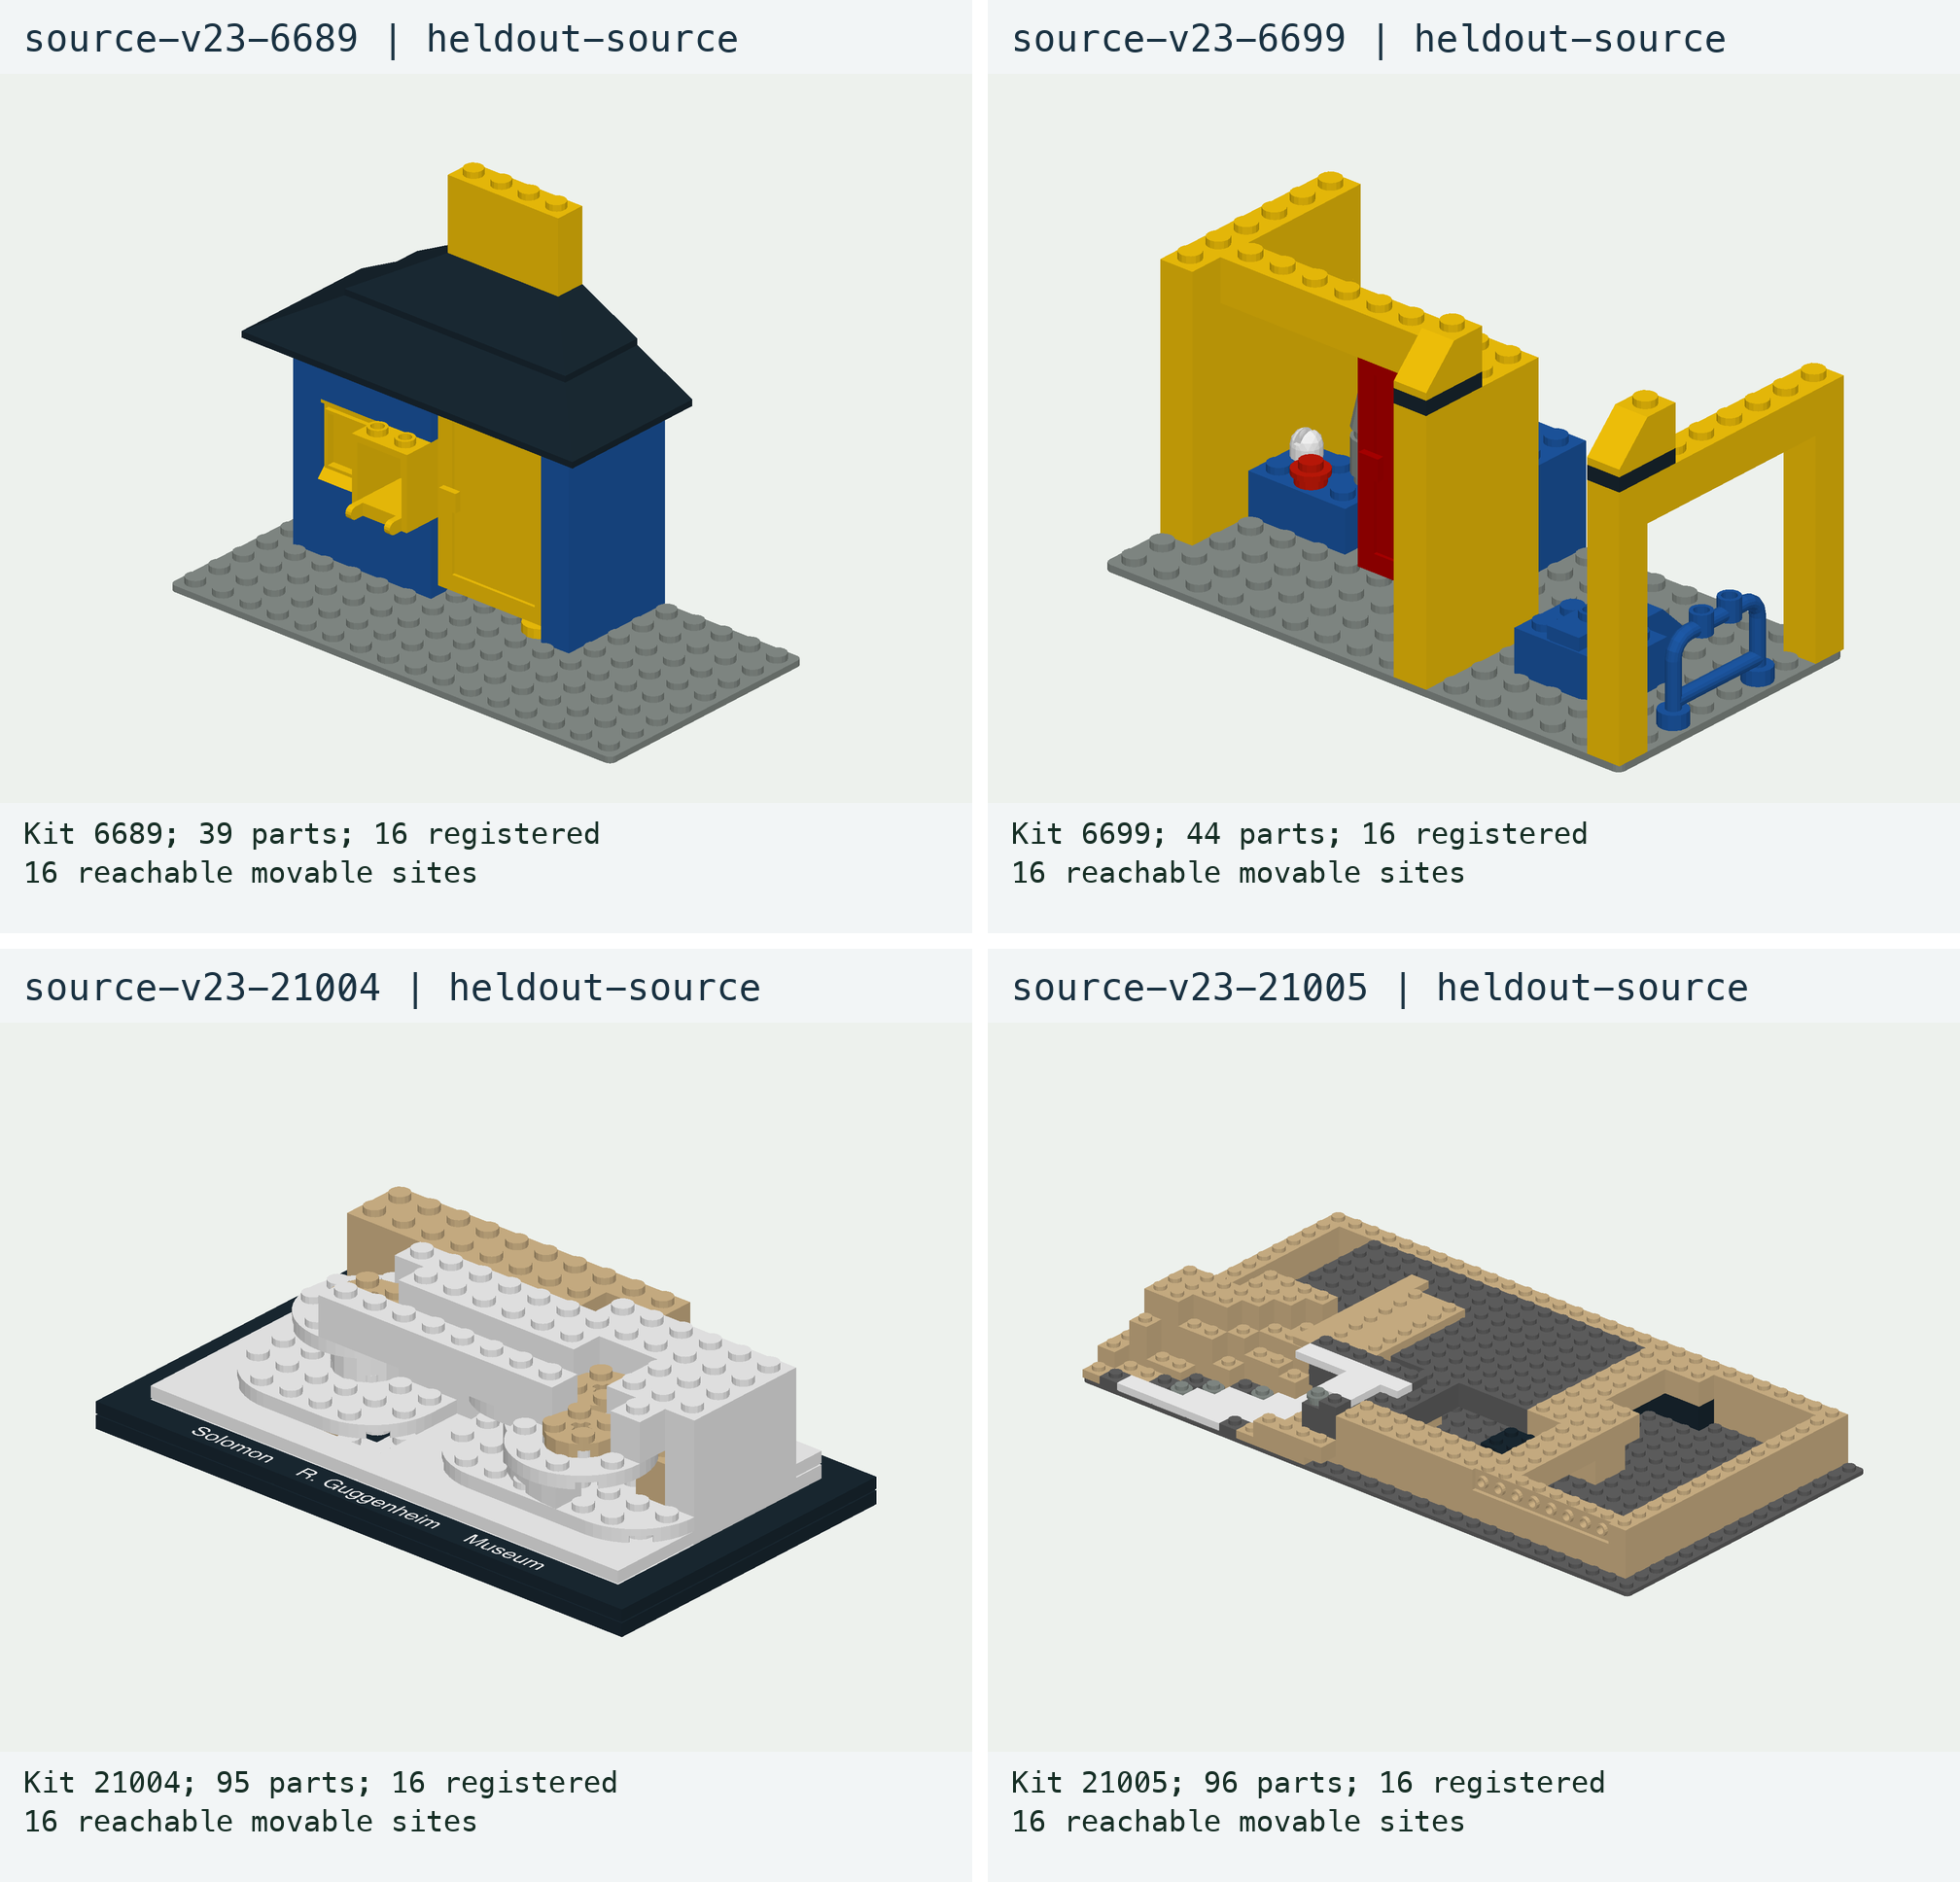
\includegraphics[width=.96\textwidth,height=.85\textheight,keepaspectratio]{figures/source-gallery-9.png}
\end{center}
\clearpage
\section*{Original-source gallery: assemblies 37--40}
\begin{center}
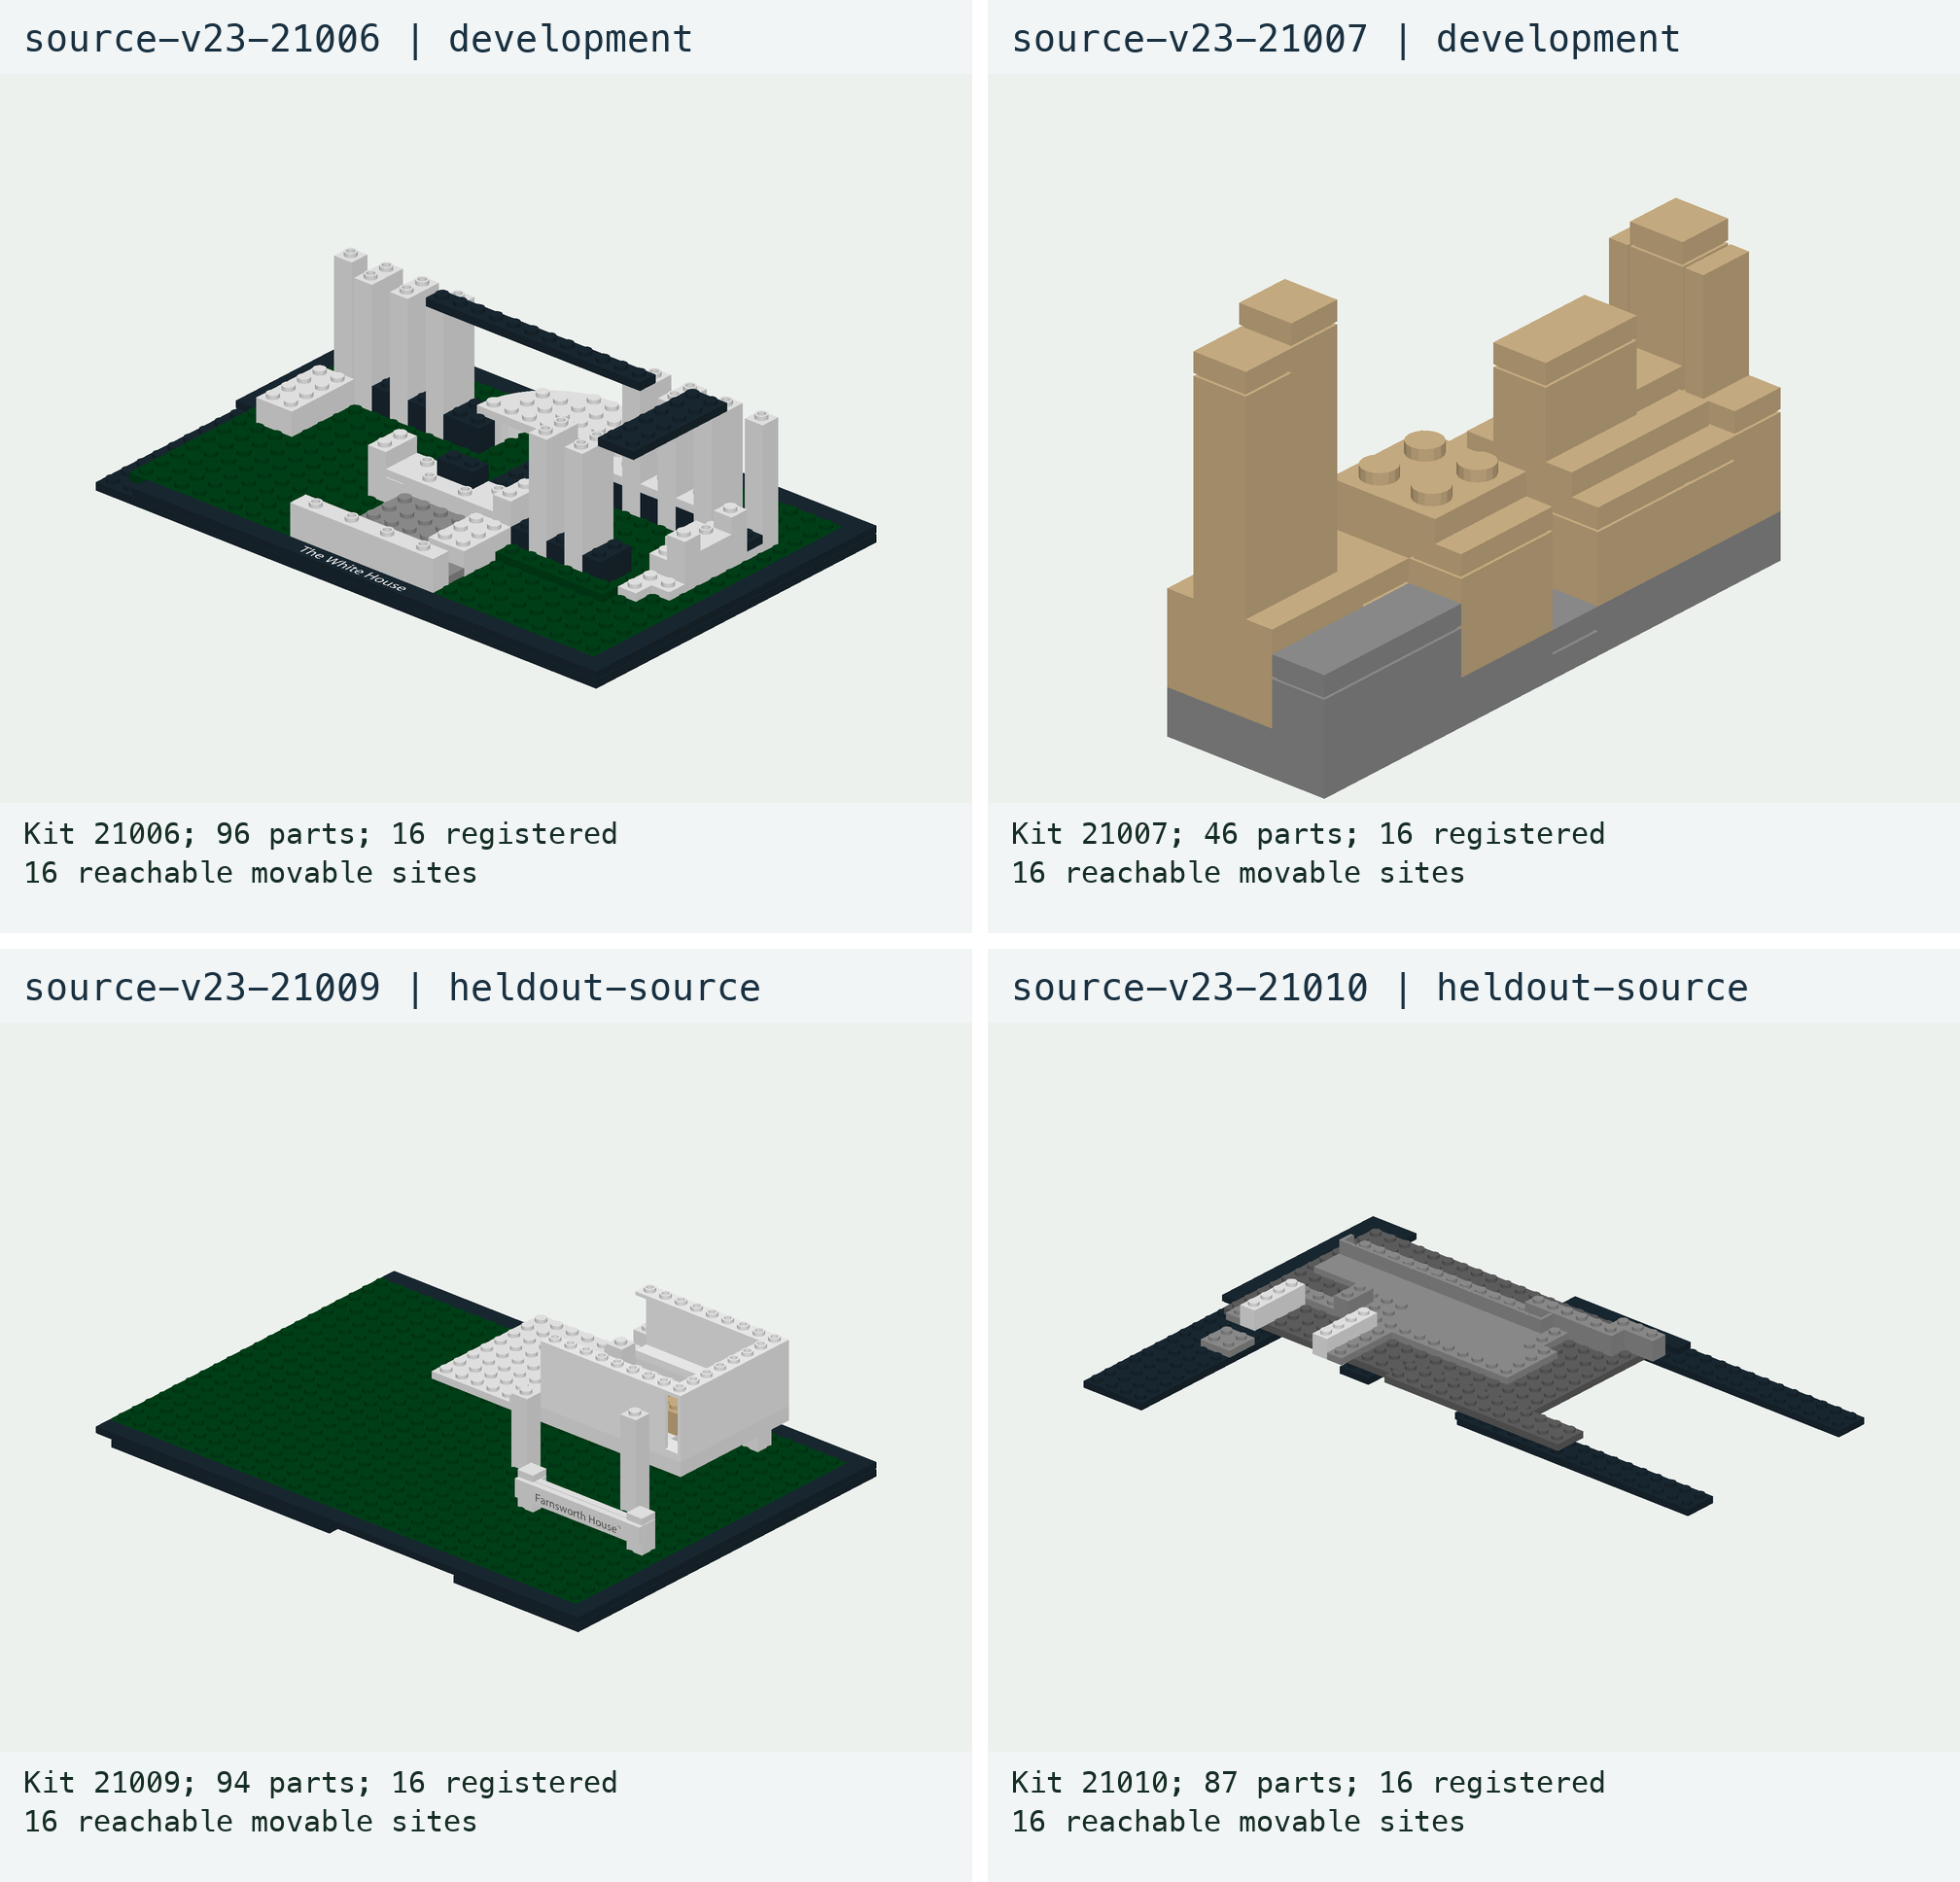
\includegraphics[width=.96\textwidth,height=.85\textheight,keepaspectratio]{figures/source-gallery-10.png}
\end{center}
\clearpage
\section*{Original-source gallery: assemblies 41--44}
\begin{center}
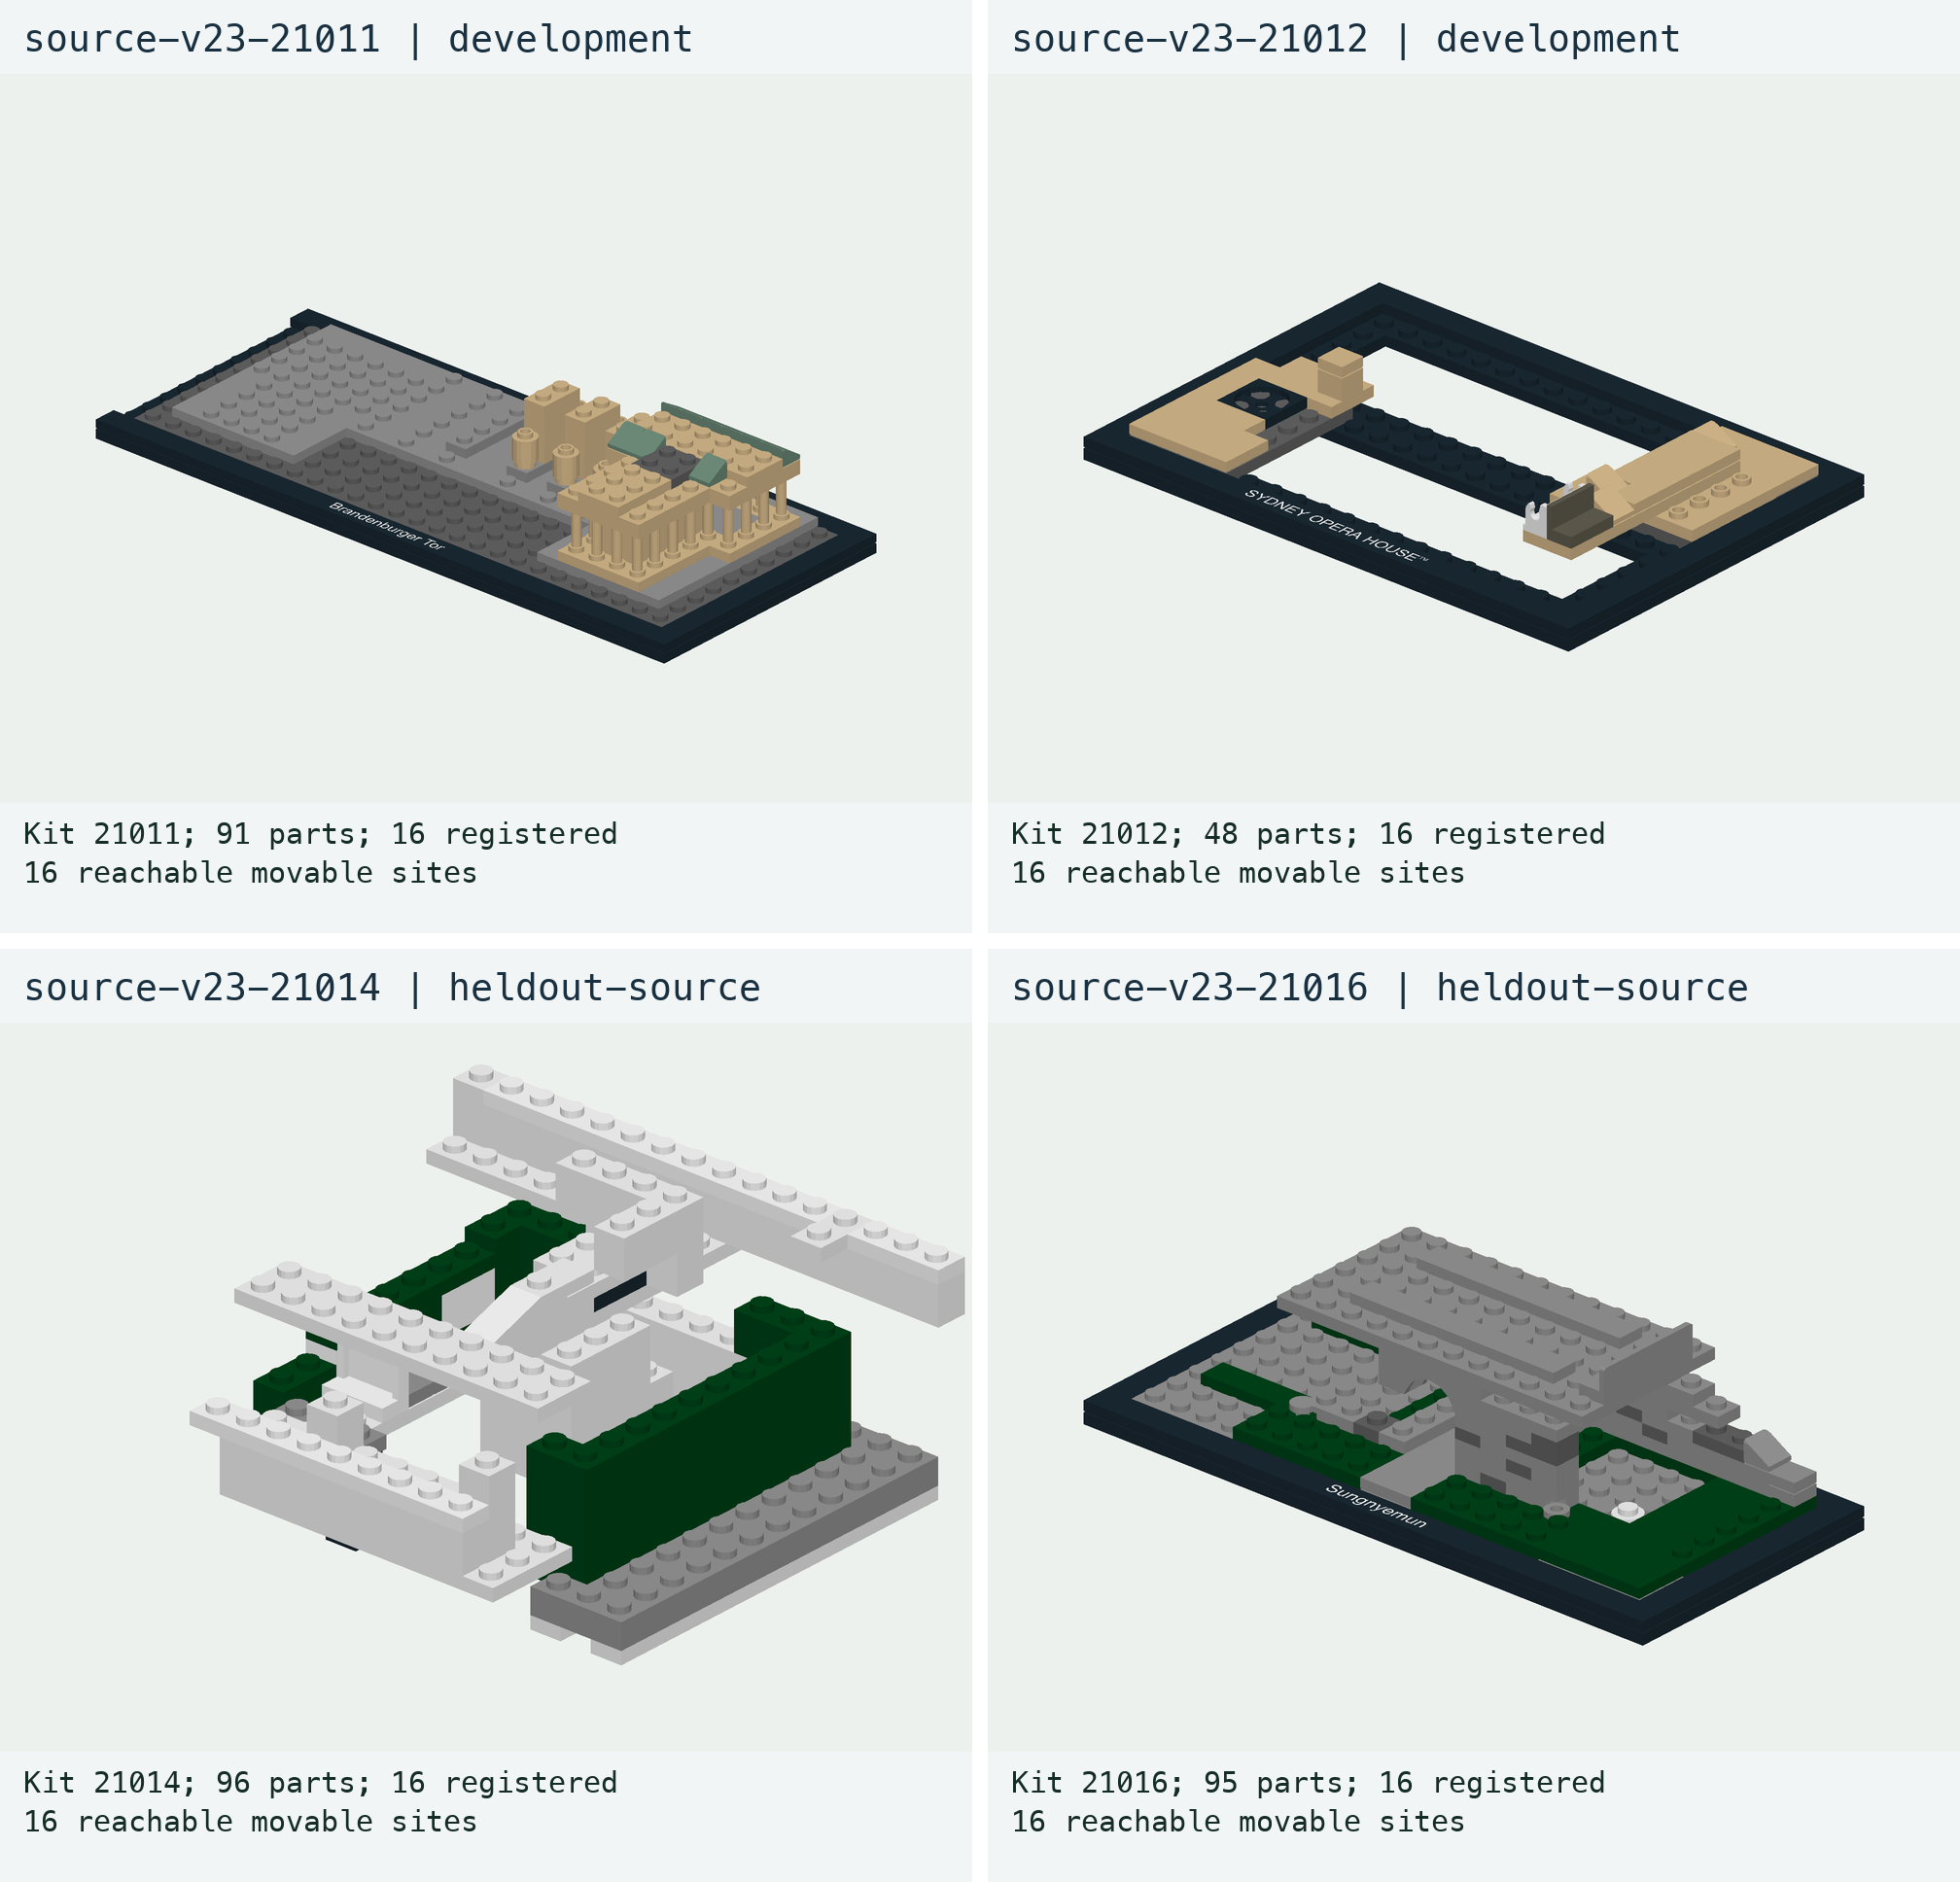
\includegraphics[width=.96\textwidth,height=.85\textheight,keepaspectratio]{figures/source-gallery-11.png}
\end{center}
\clearpage
\section*{Original-source gallery: assemblies 45--48}
\begin{center}
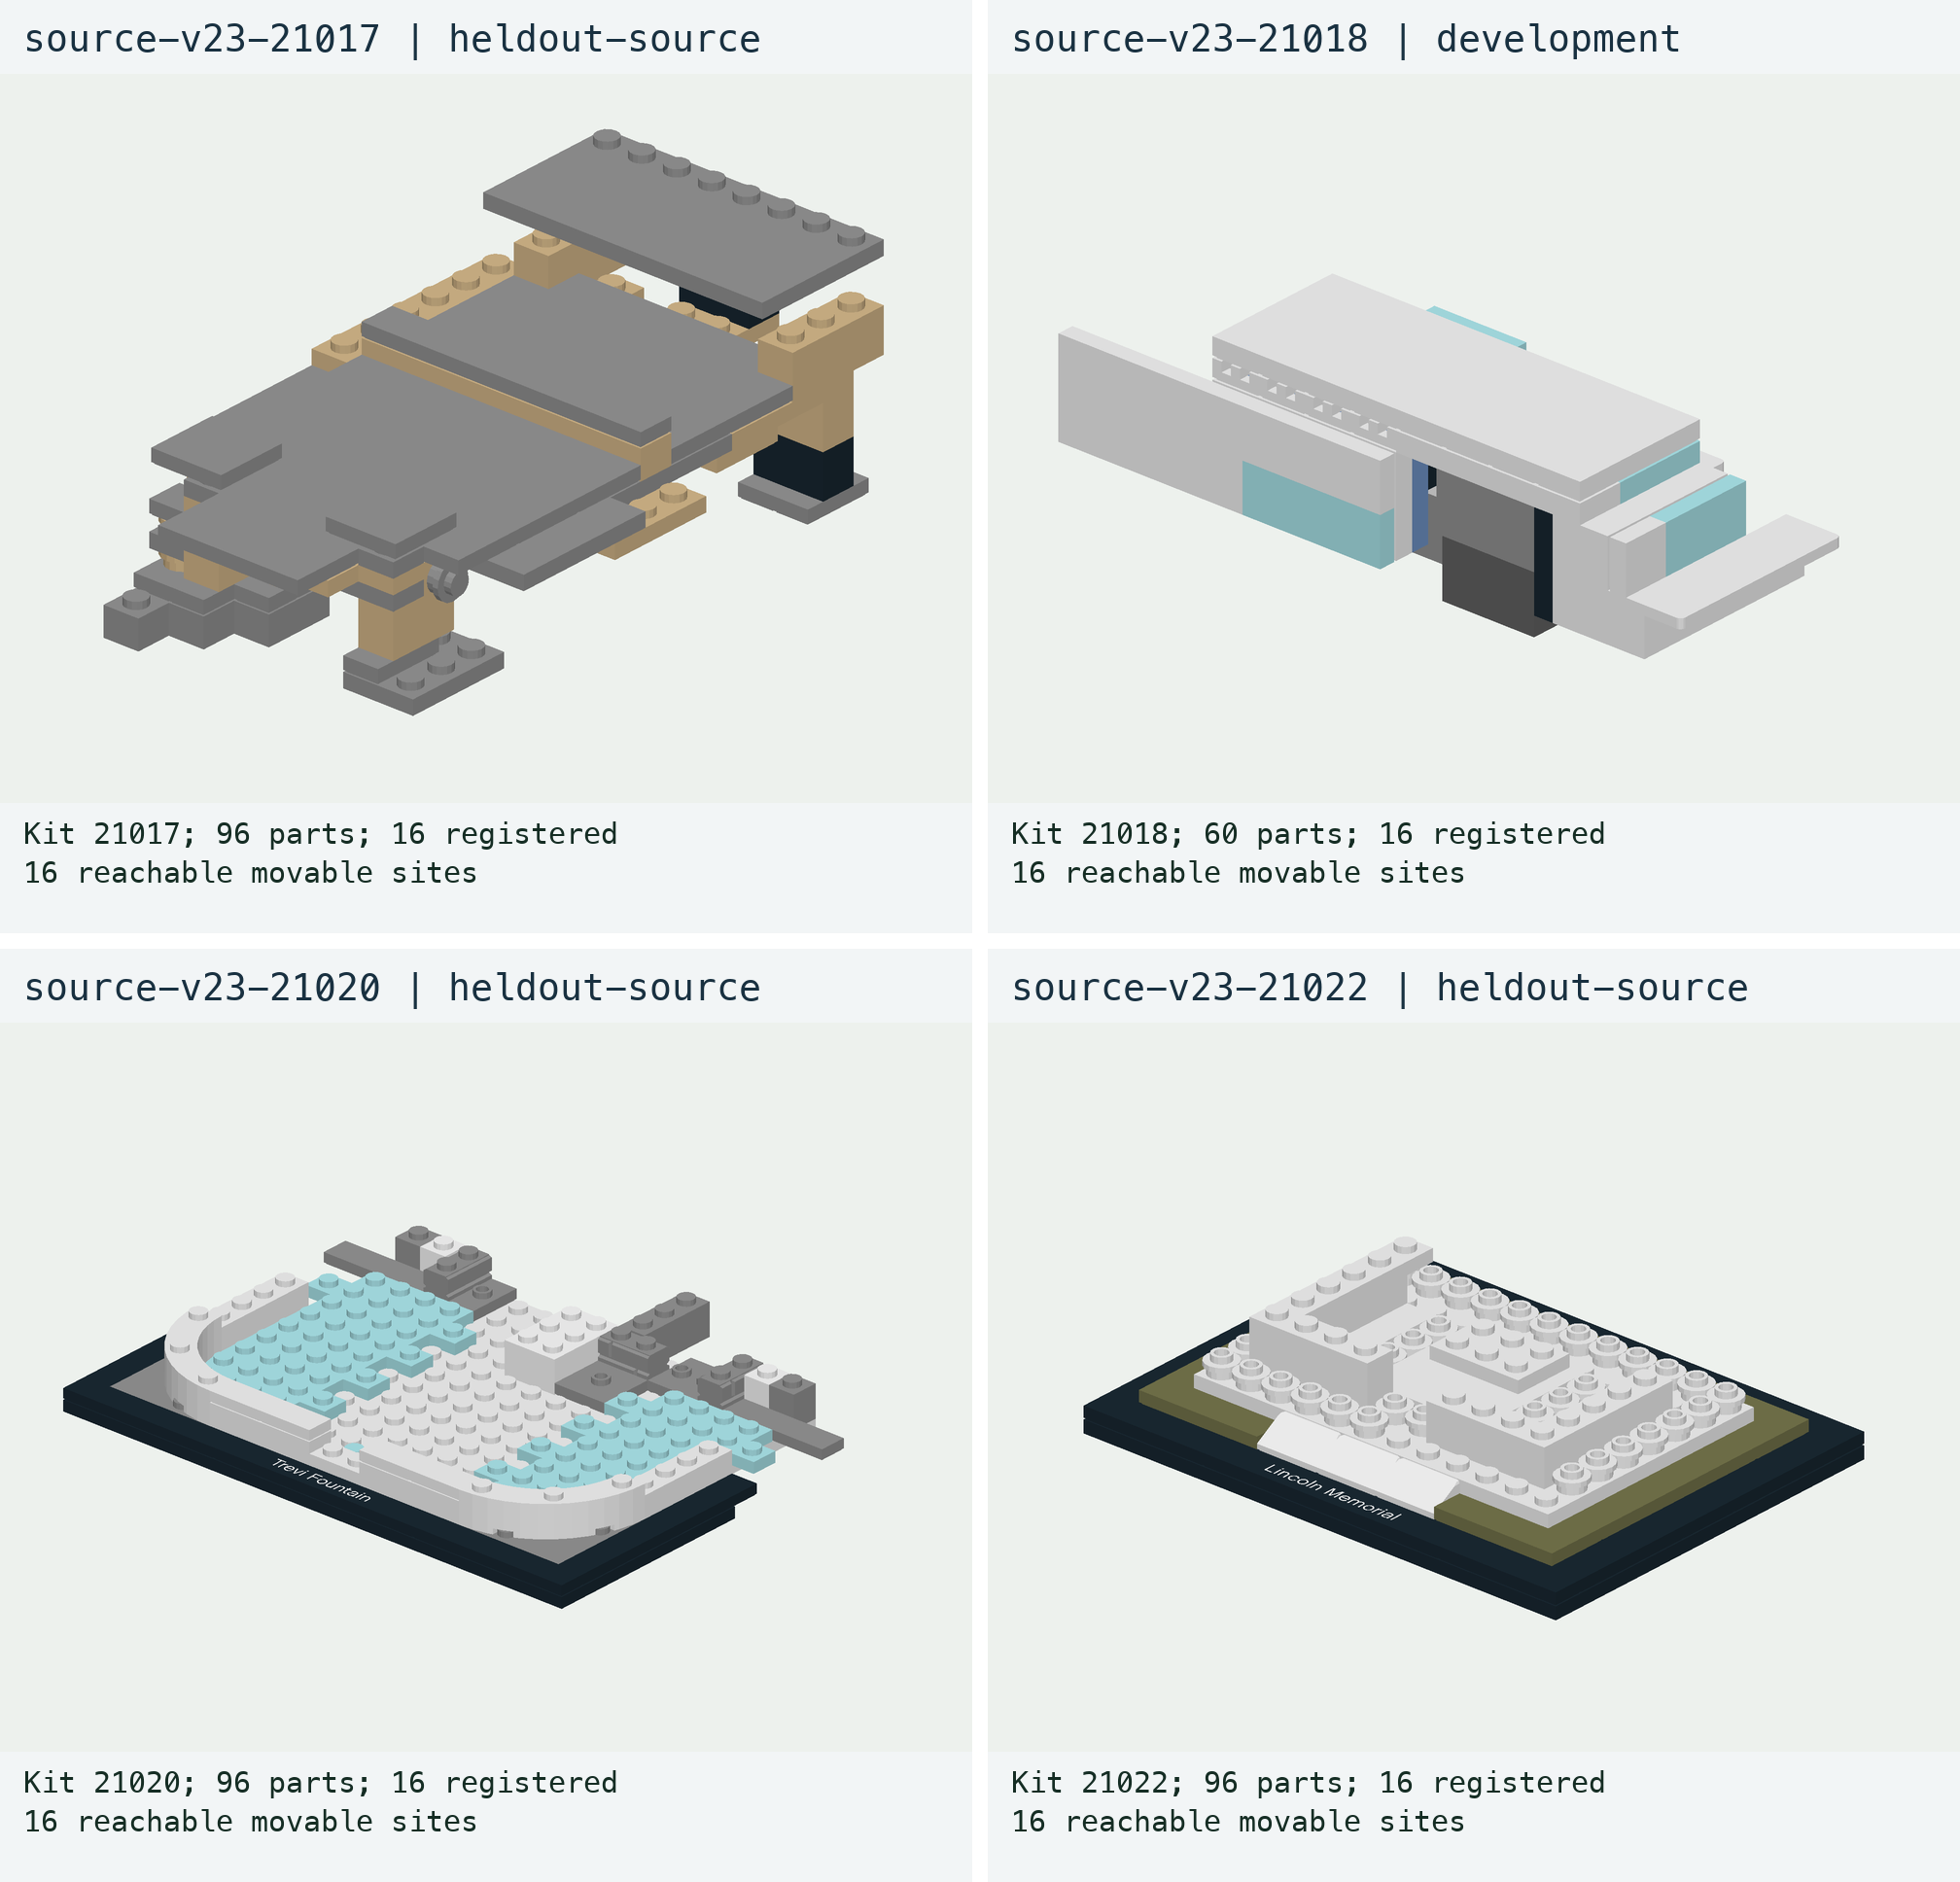
\includegraphics[width=.96\textwidth,height=.85\textheight,keepaspectratio]{figures/source-gallery-12.png}
\end{center}
\clearpage
\section*{Original-source gallery: assemblies 49--52}
\begin{center}
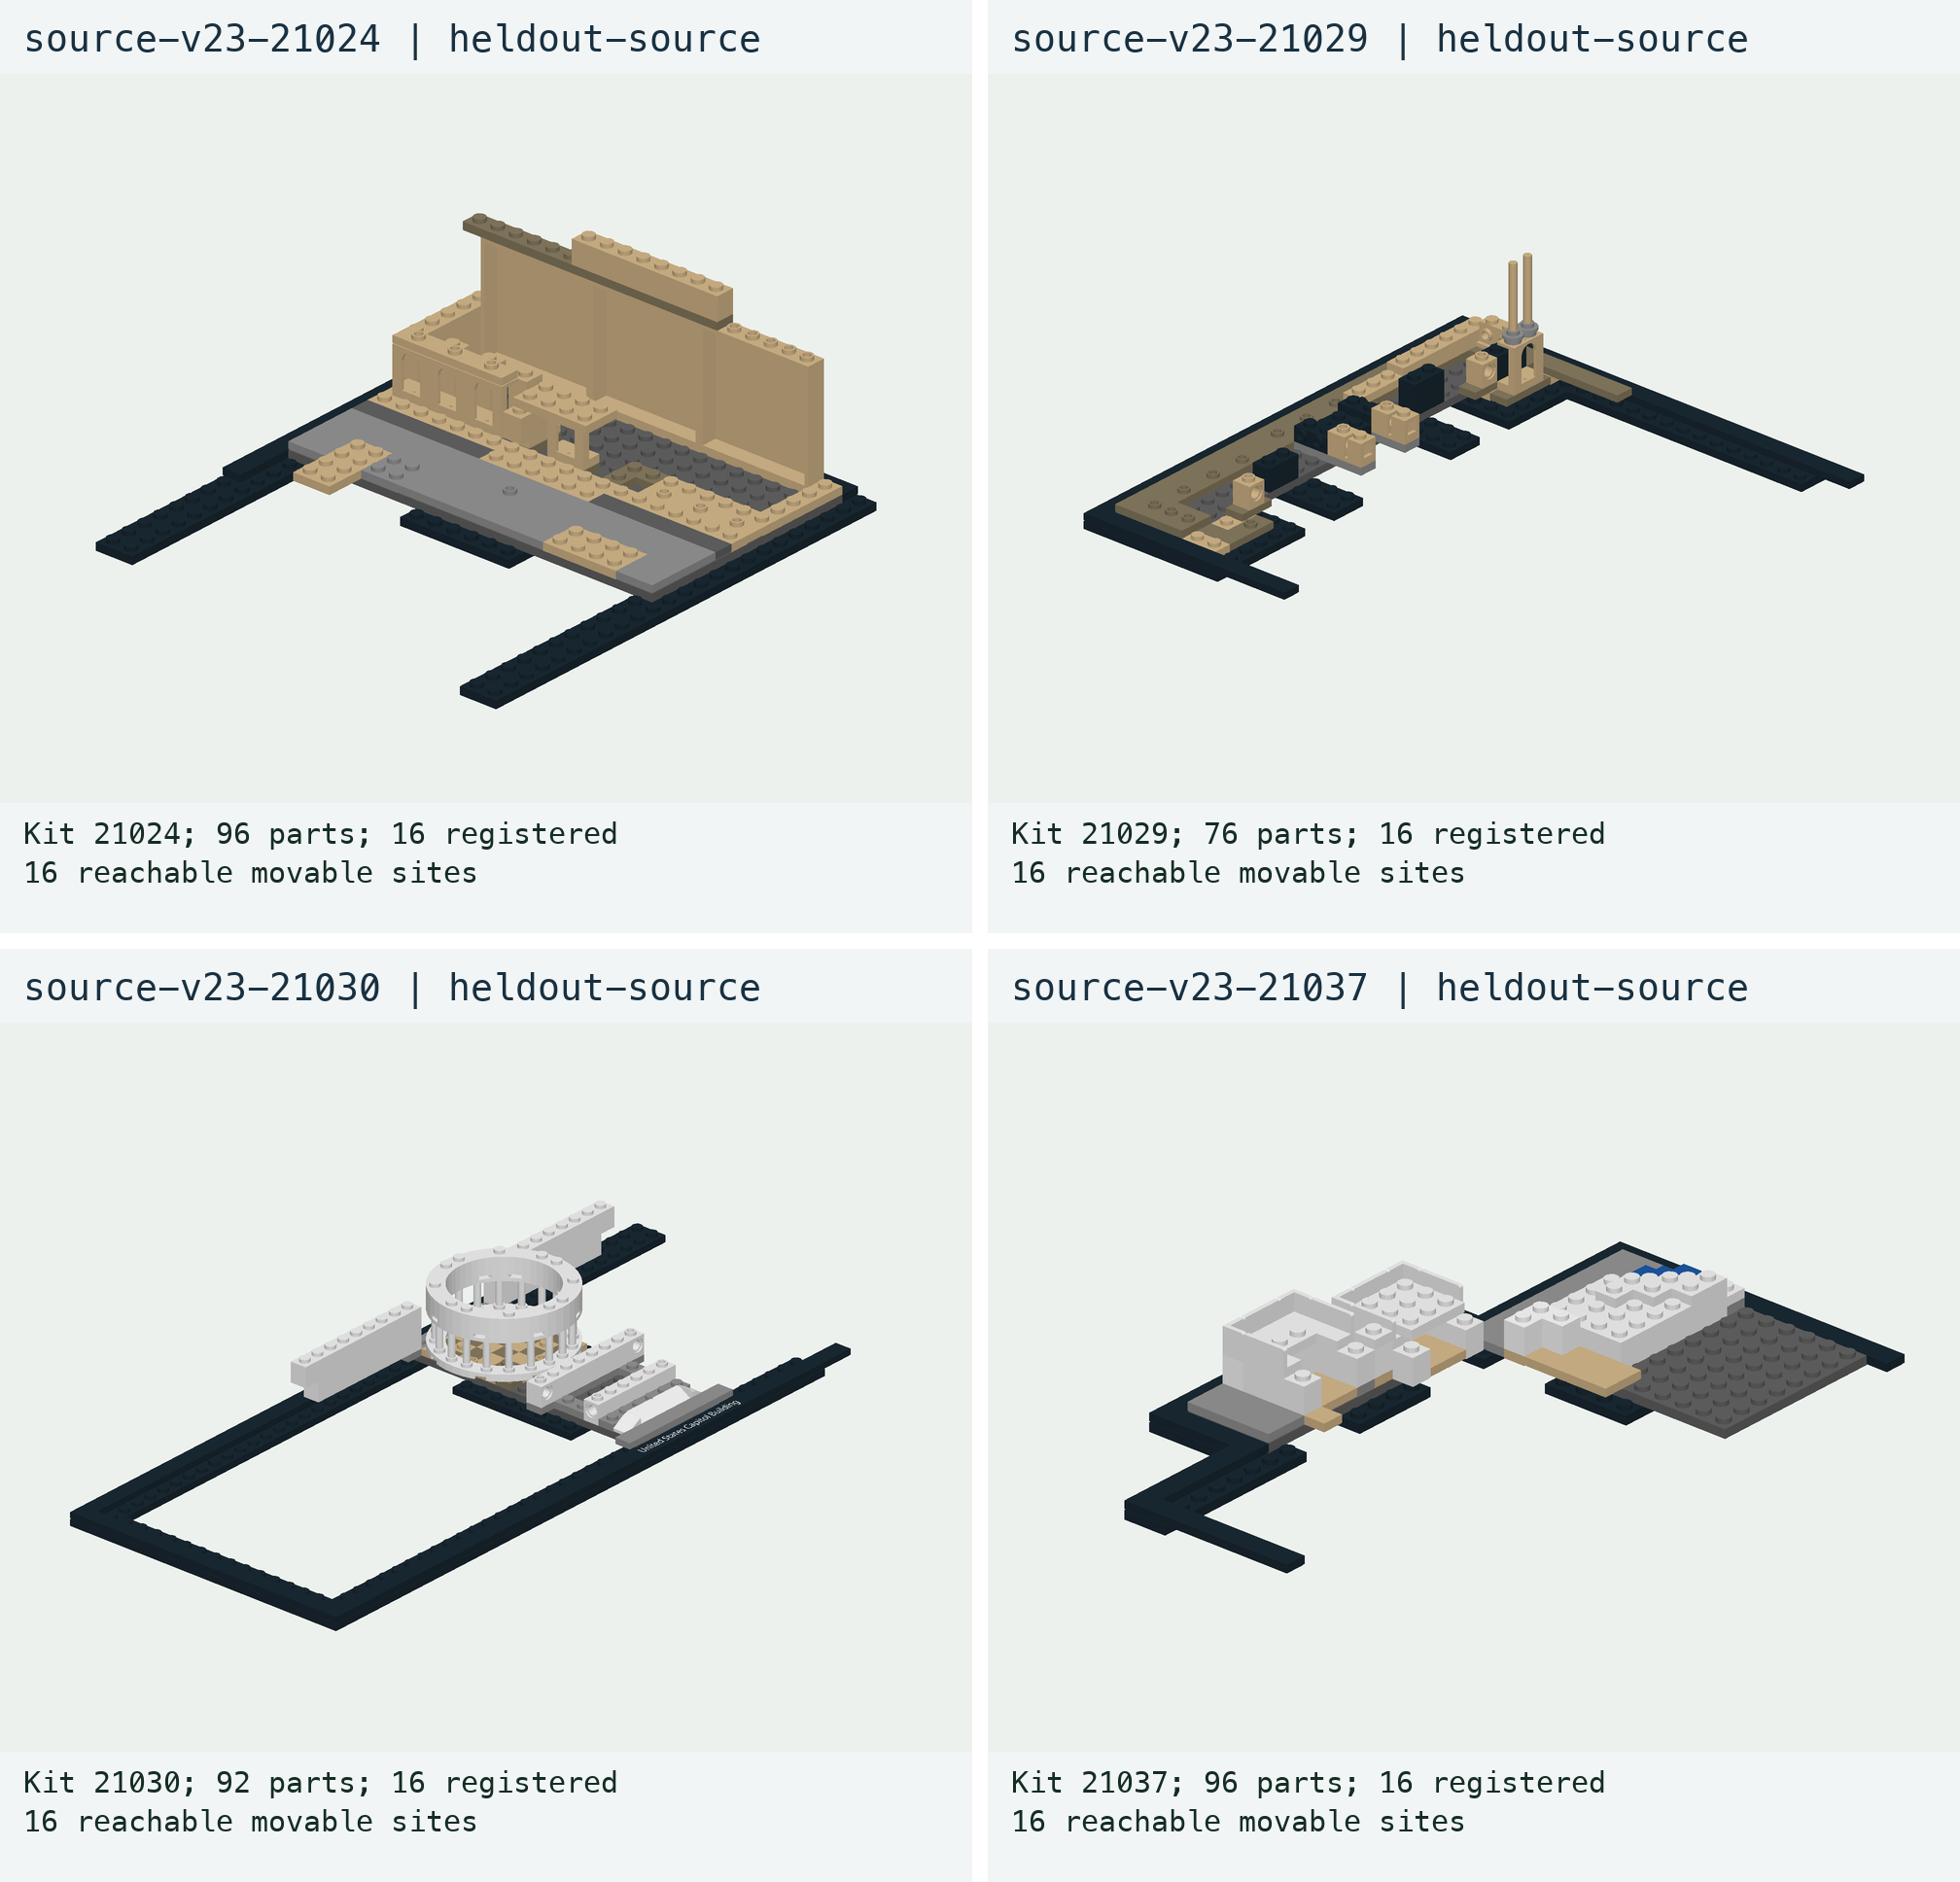
\includegraphics[width=.96\textwidth,height=.85\textheight,keepaspectratio]{figures/source-gallery-13.png}
\end{center}
\clearpage
\section*{Original-source gallery: assemblies 53--56}
\begin{center}
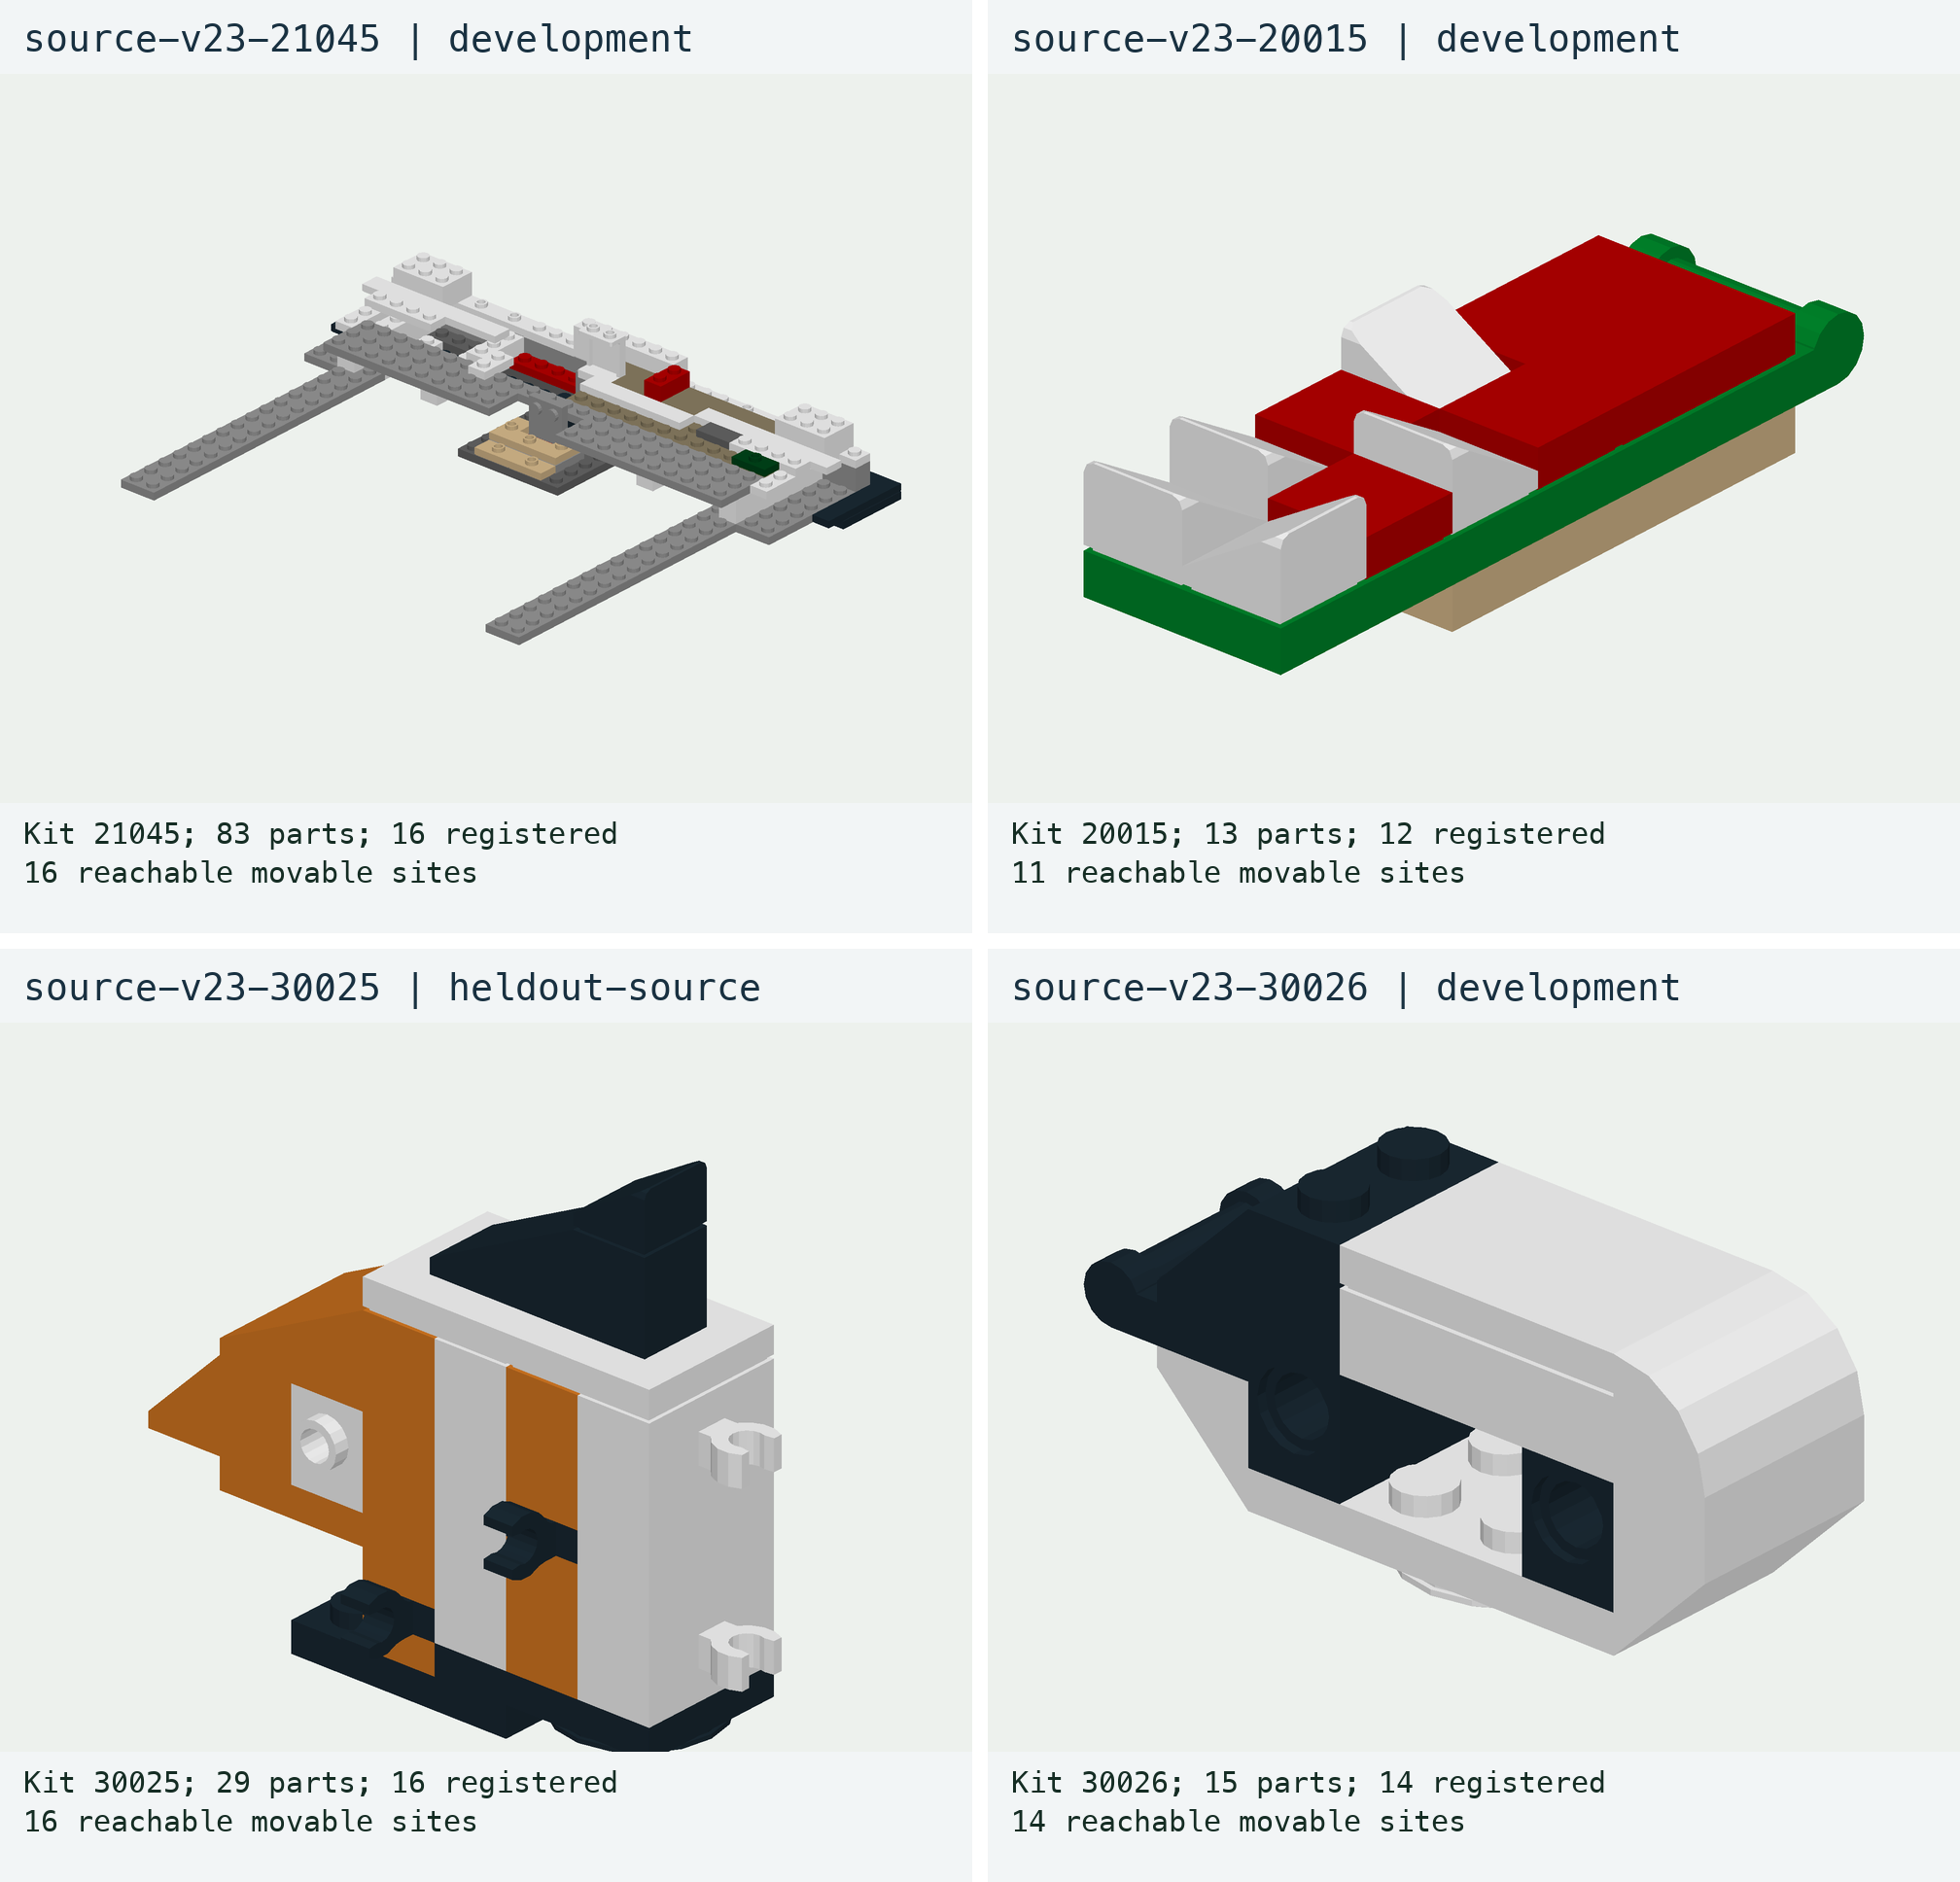
\includegraphics[width=.96\textwidth,height=.85\textheight,keepaspectratio]{figures/source-gallery-14.png}
\end{center}
\clearpage
\section*{Original-source gallery: assemblies 57--60}
\begin{center}
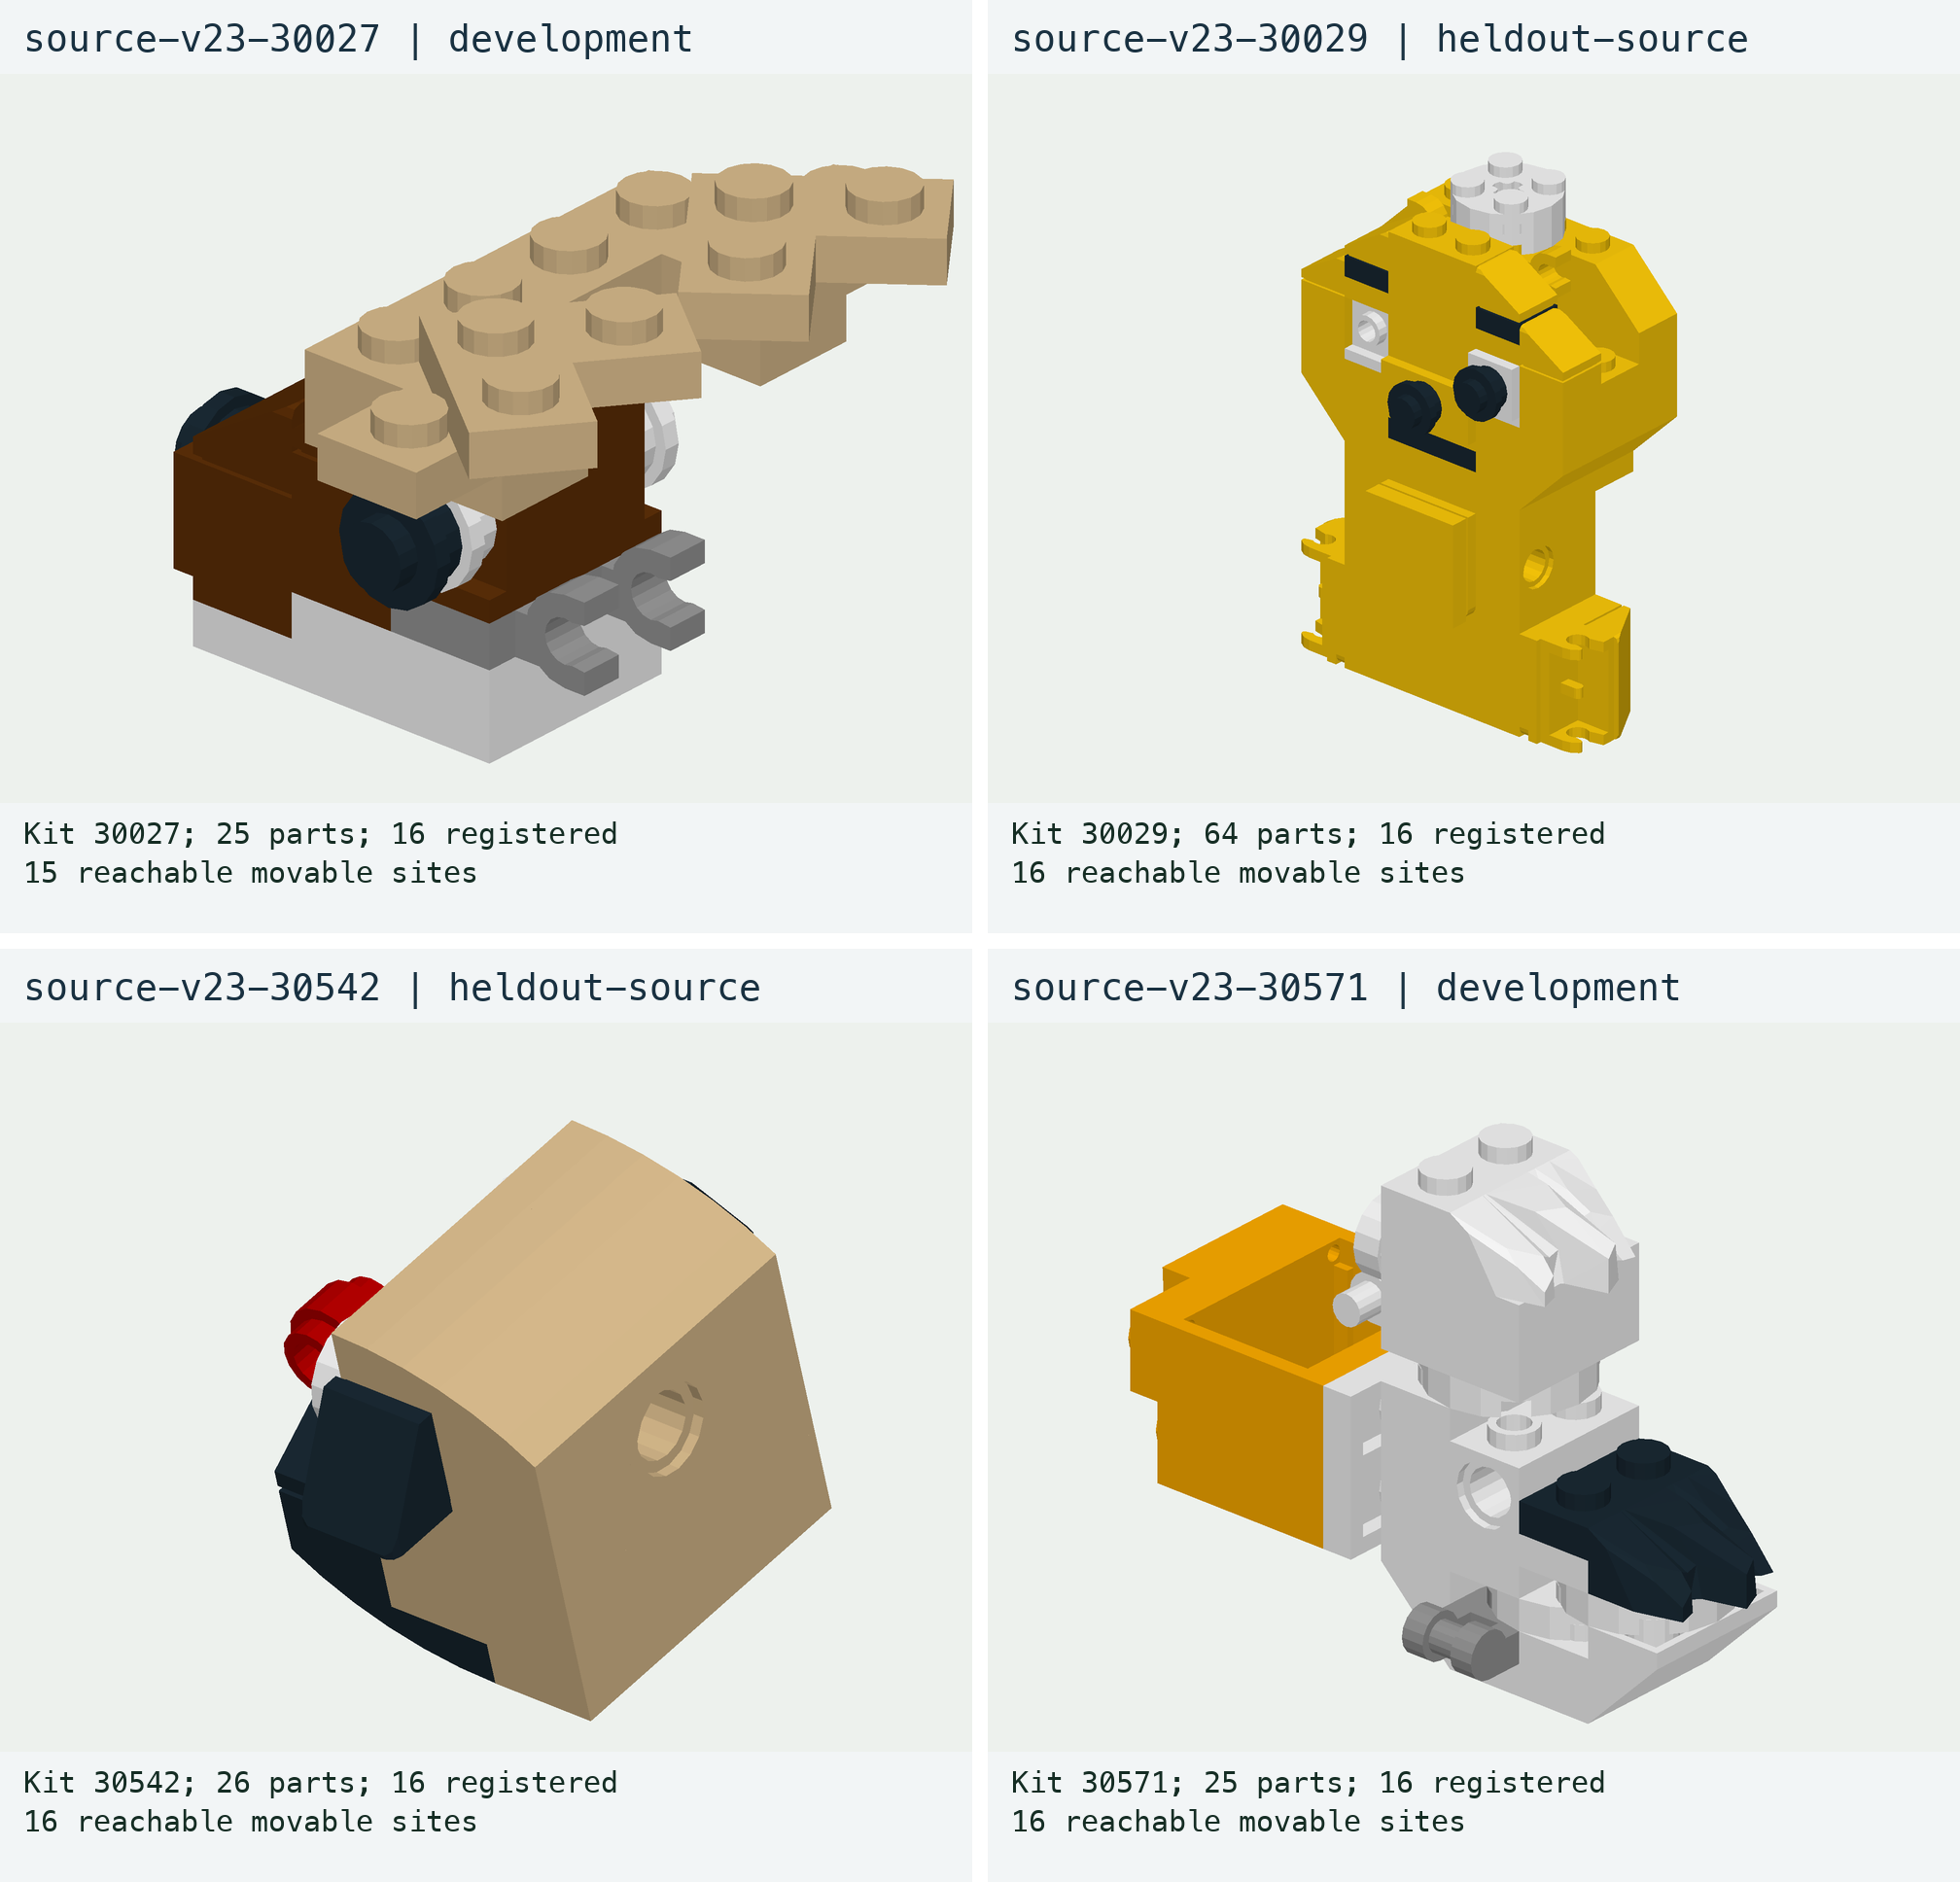
\includegraphics[width=.96\textwidth,height=.85\textheight,keepaspectratio]{figures/source-gallery-15.png}
\end{center}
\clearpage
\section*{Original-source gallery: assemblies 61--64}
\begin{center}
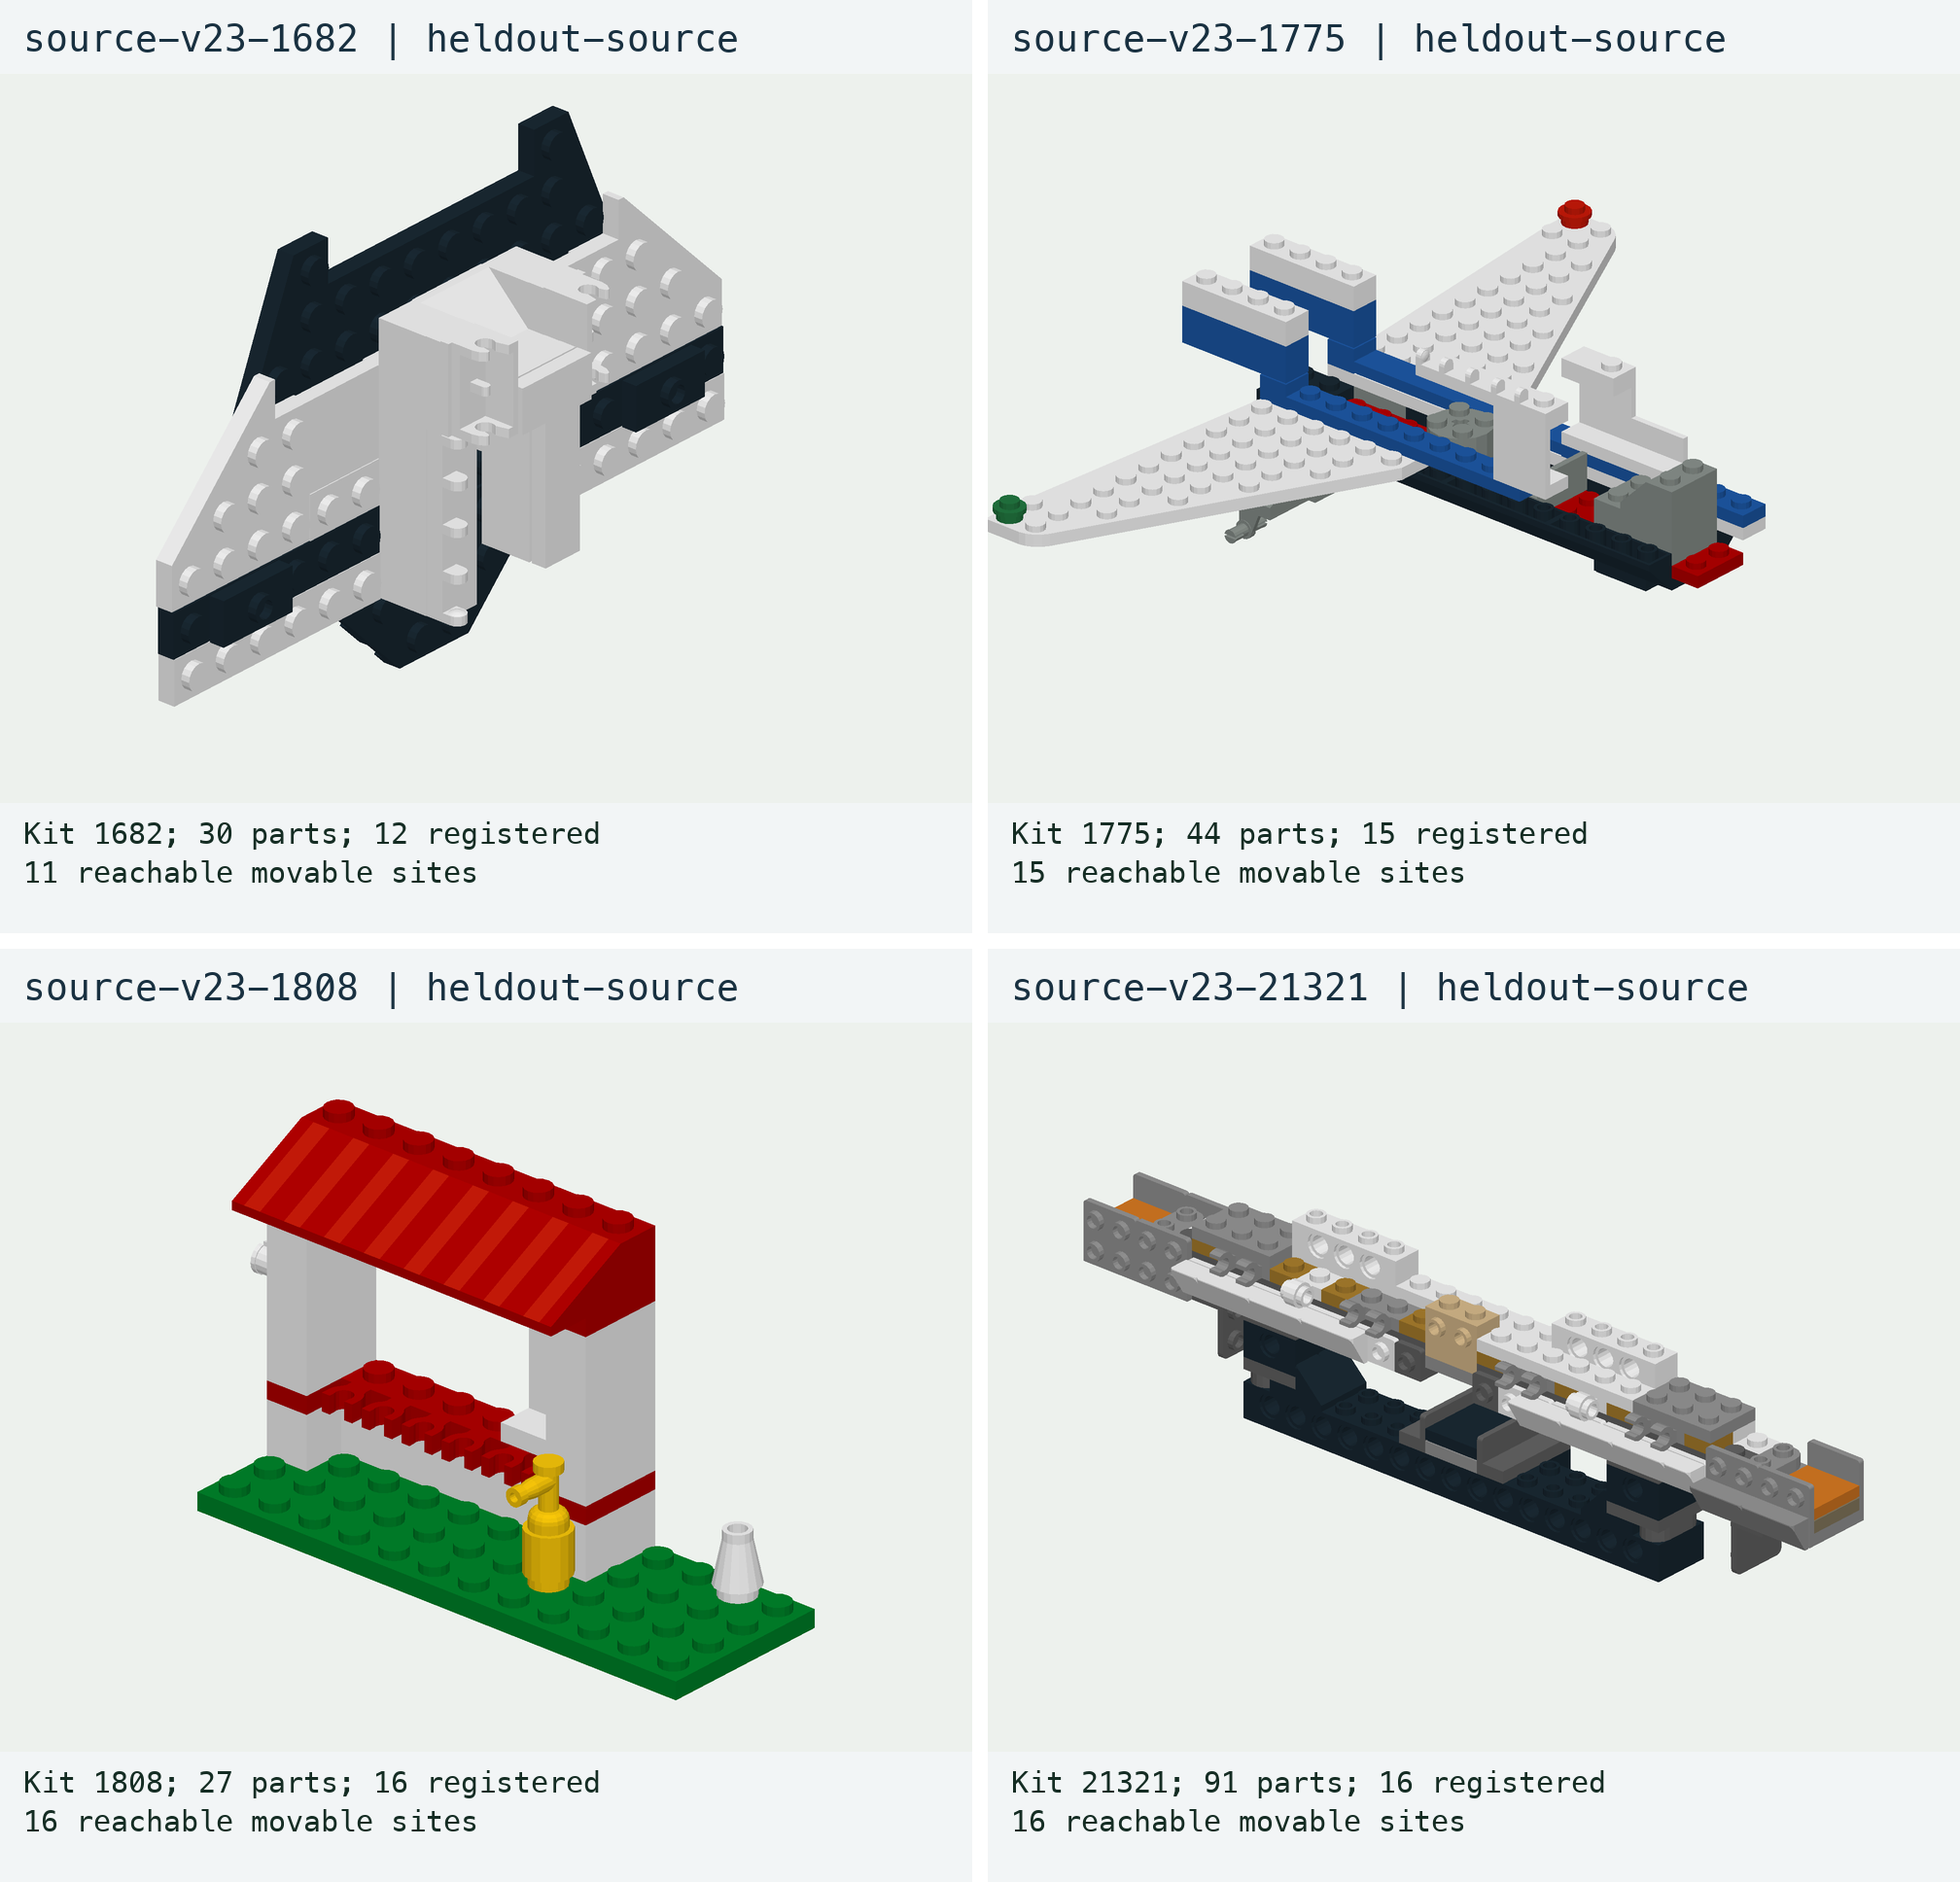
\includegraphics[width=.96\textwidth,height=.85\textheight,keepaspectratio]{figures/source-gallery-16.png}
\end{center}
\clearpage
\section*{Original-source gallery: assemblies 65--68}
\begin{center}
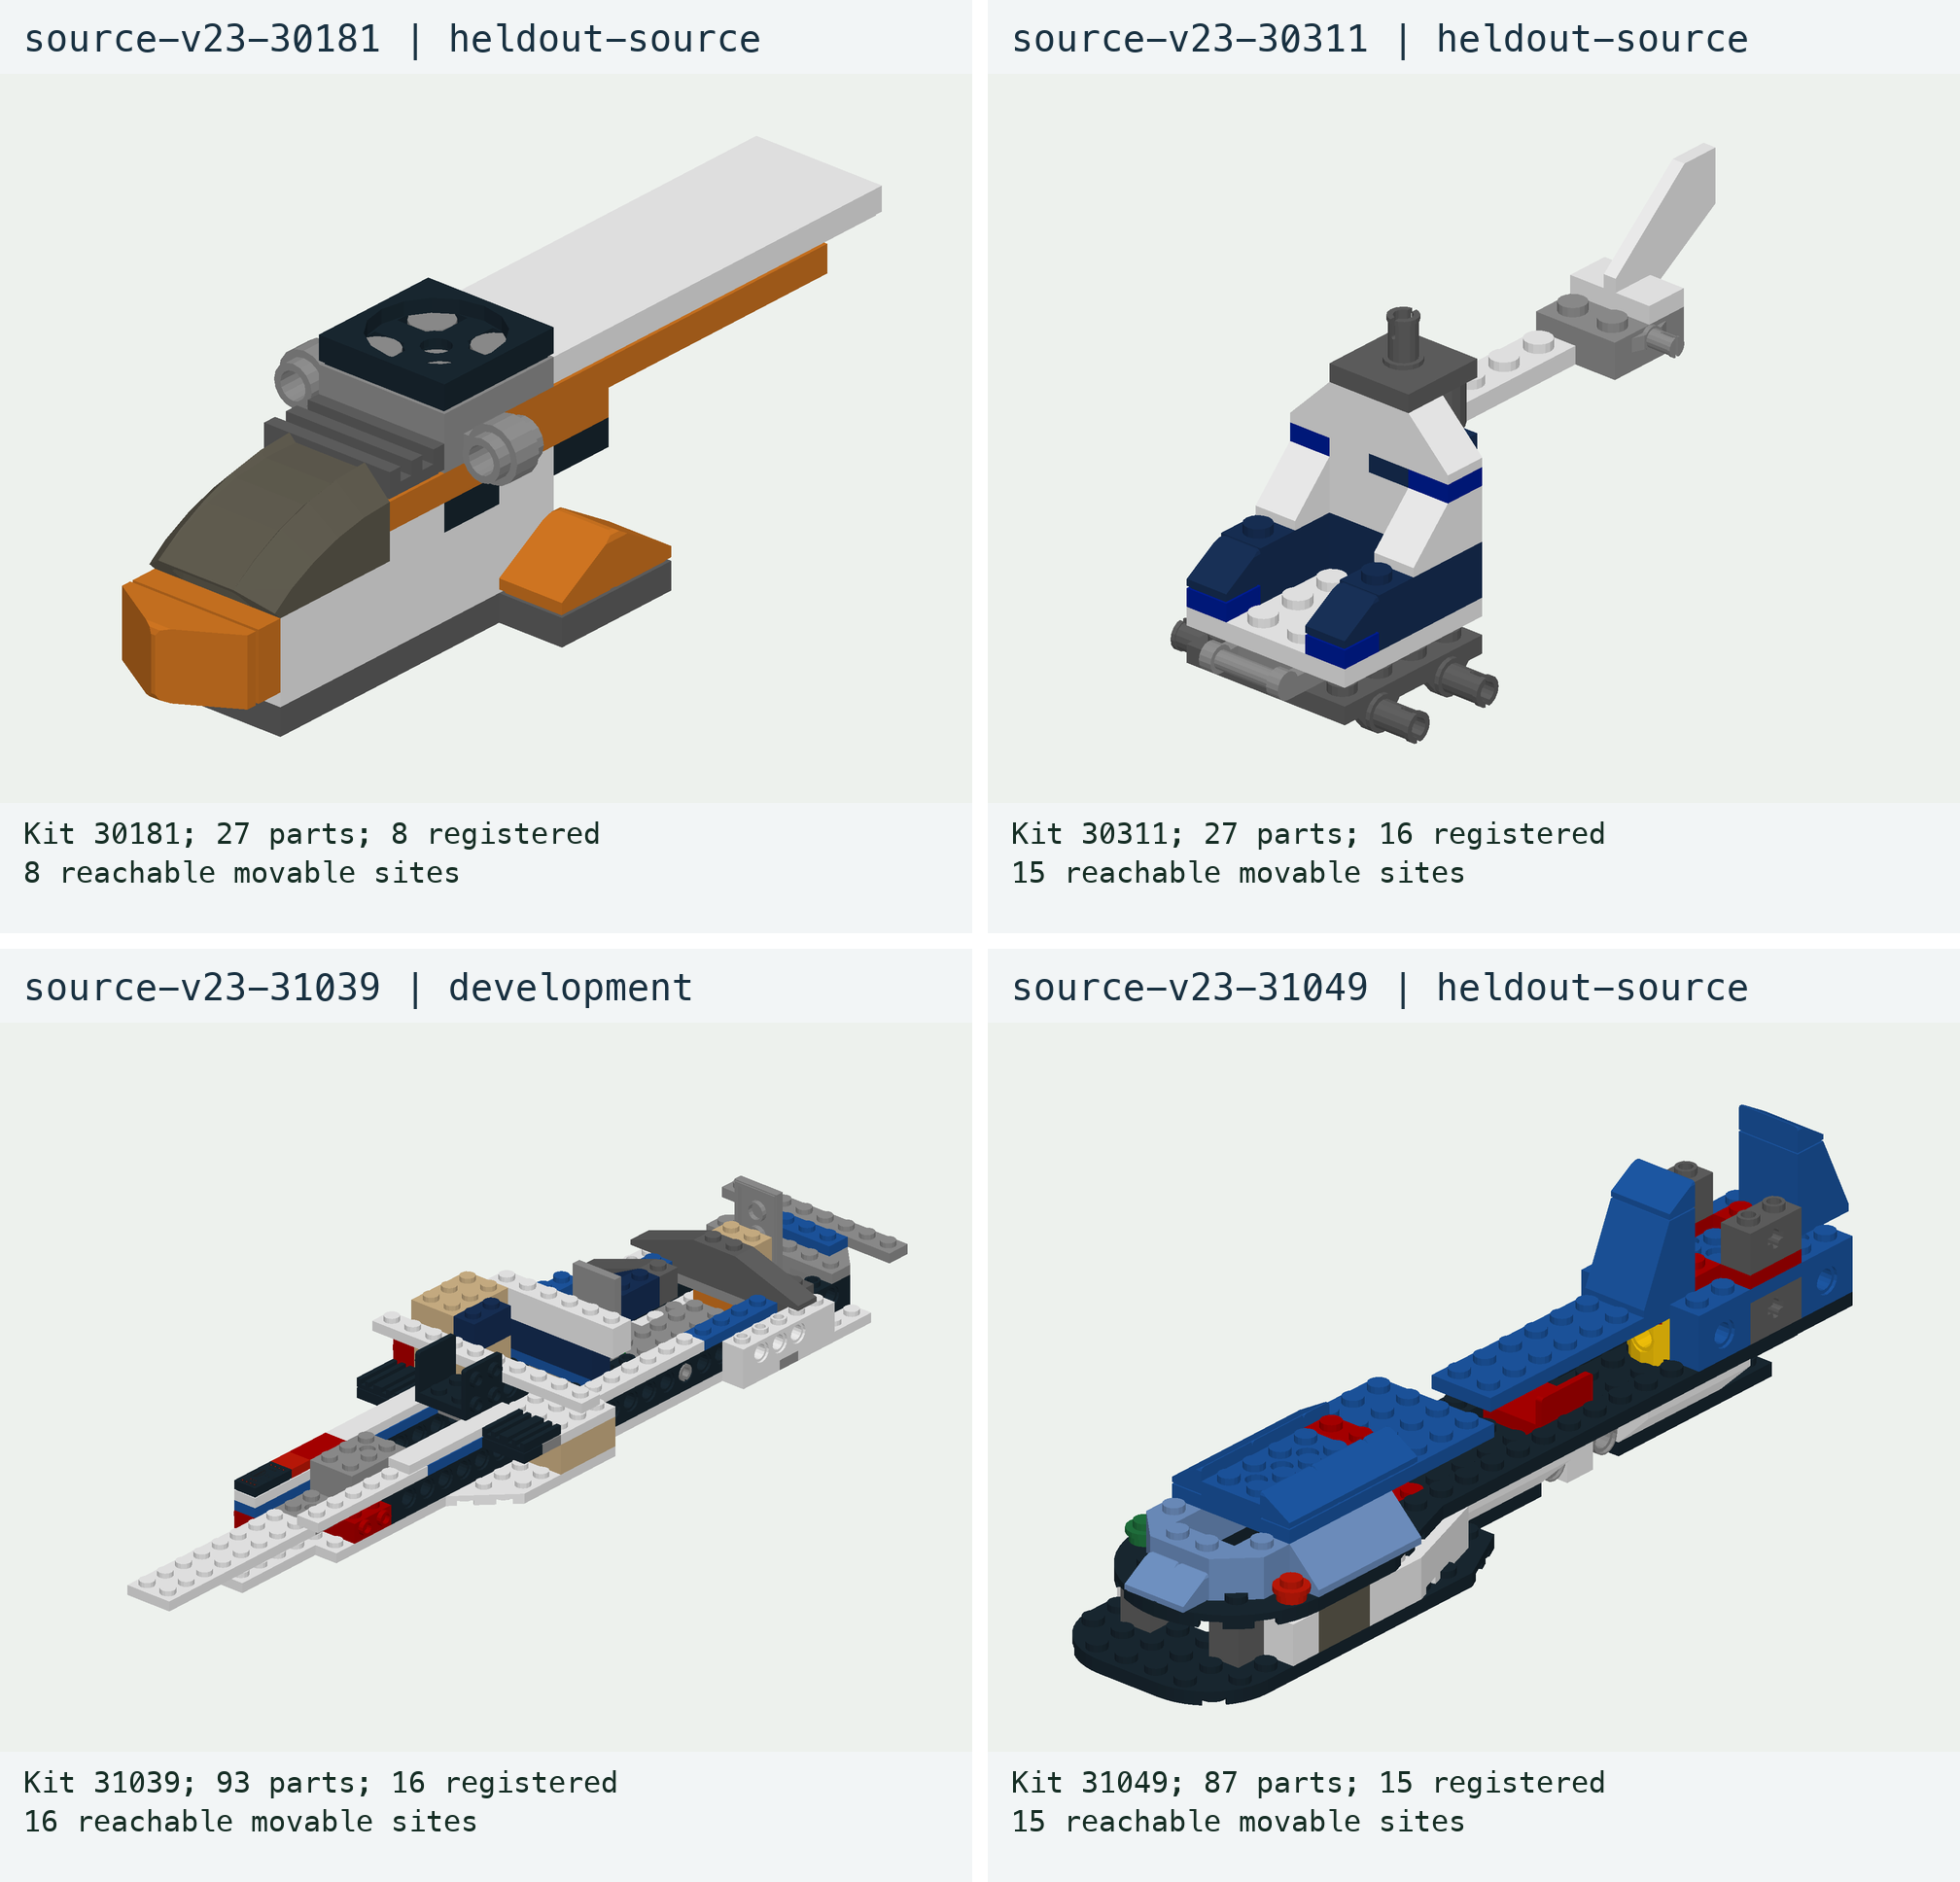
\includegraphics[width=.96\textwidth,height=.85\textheight,keepaspectratio]{figures/source-gallery-17.png}
\end{center}
\clearpage
\section*{Original-source gallery: assemblies 69--72}
\begin{center}
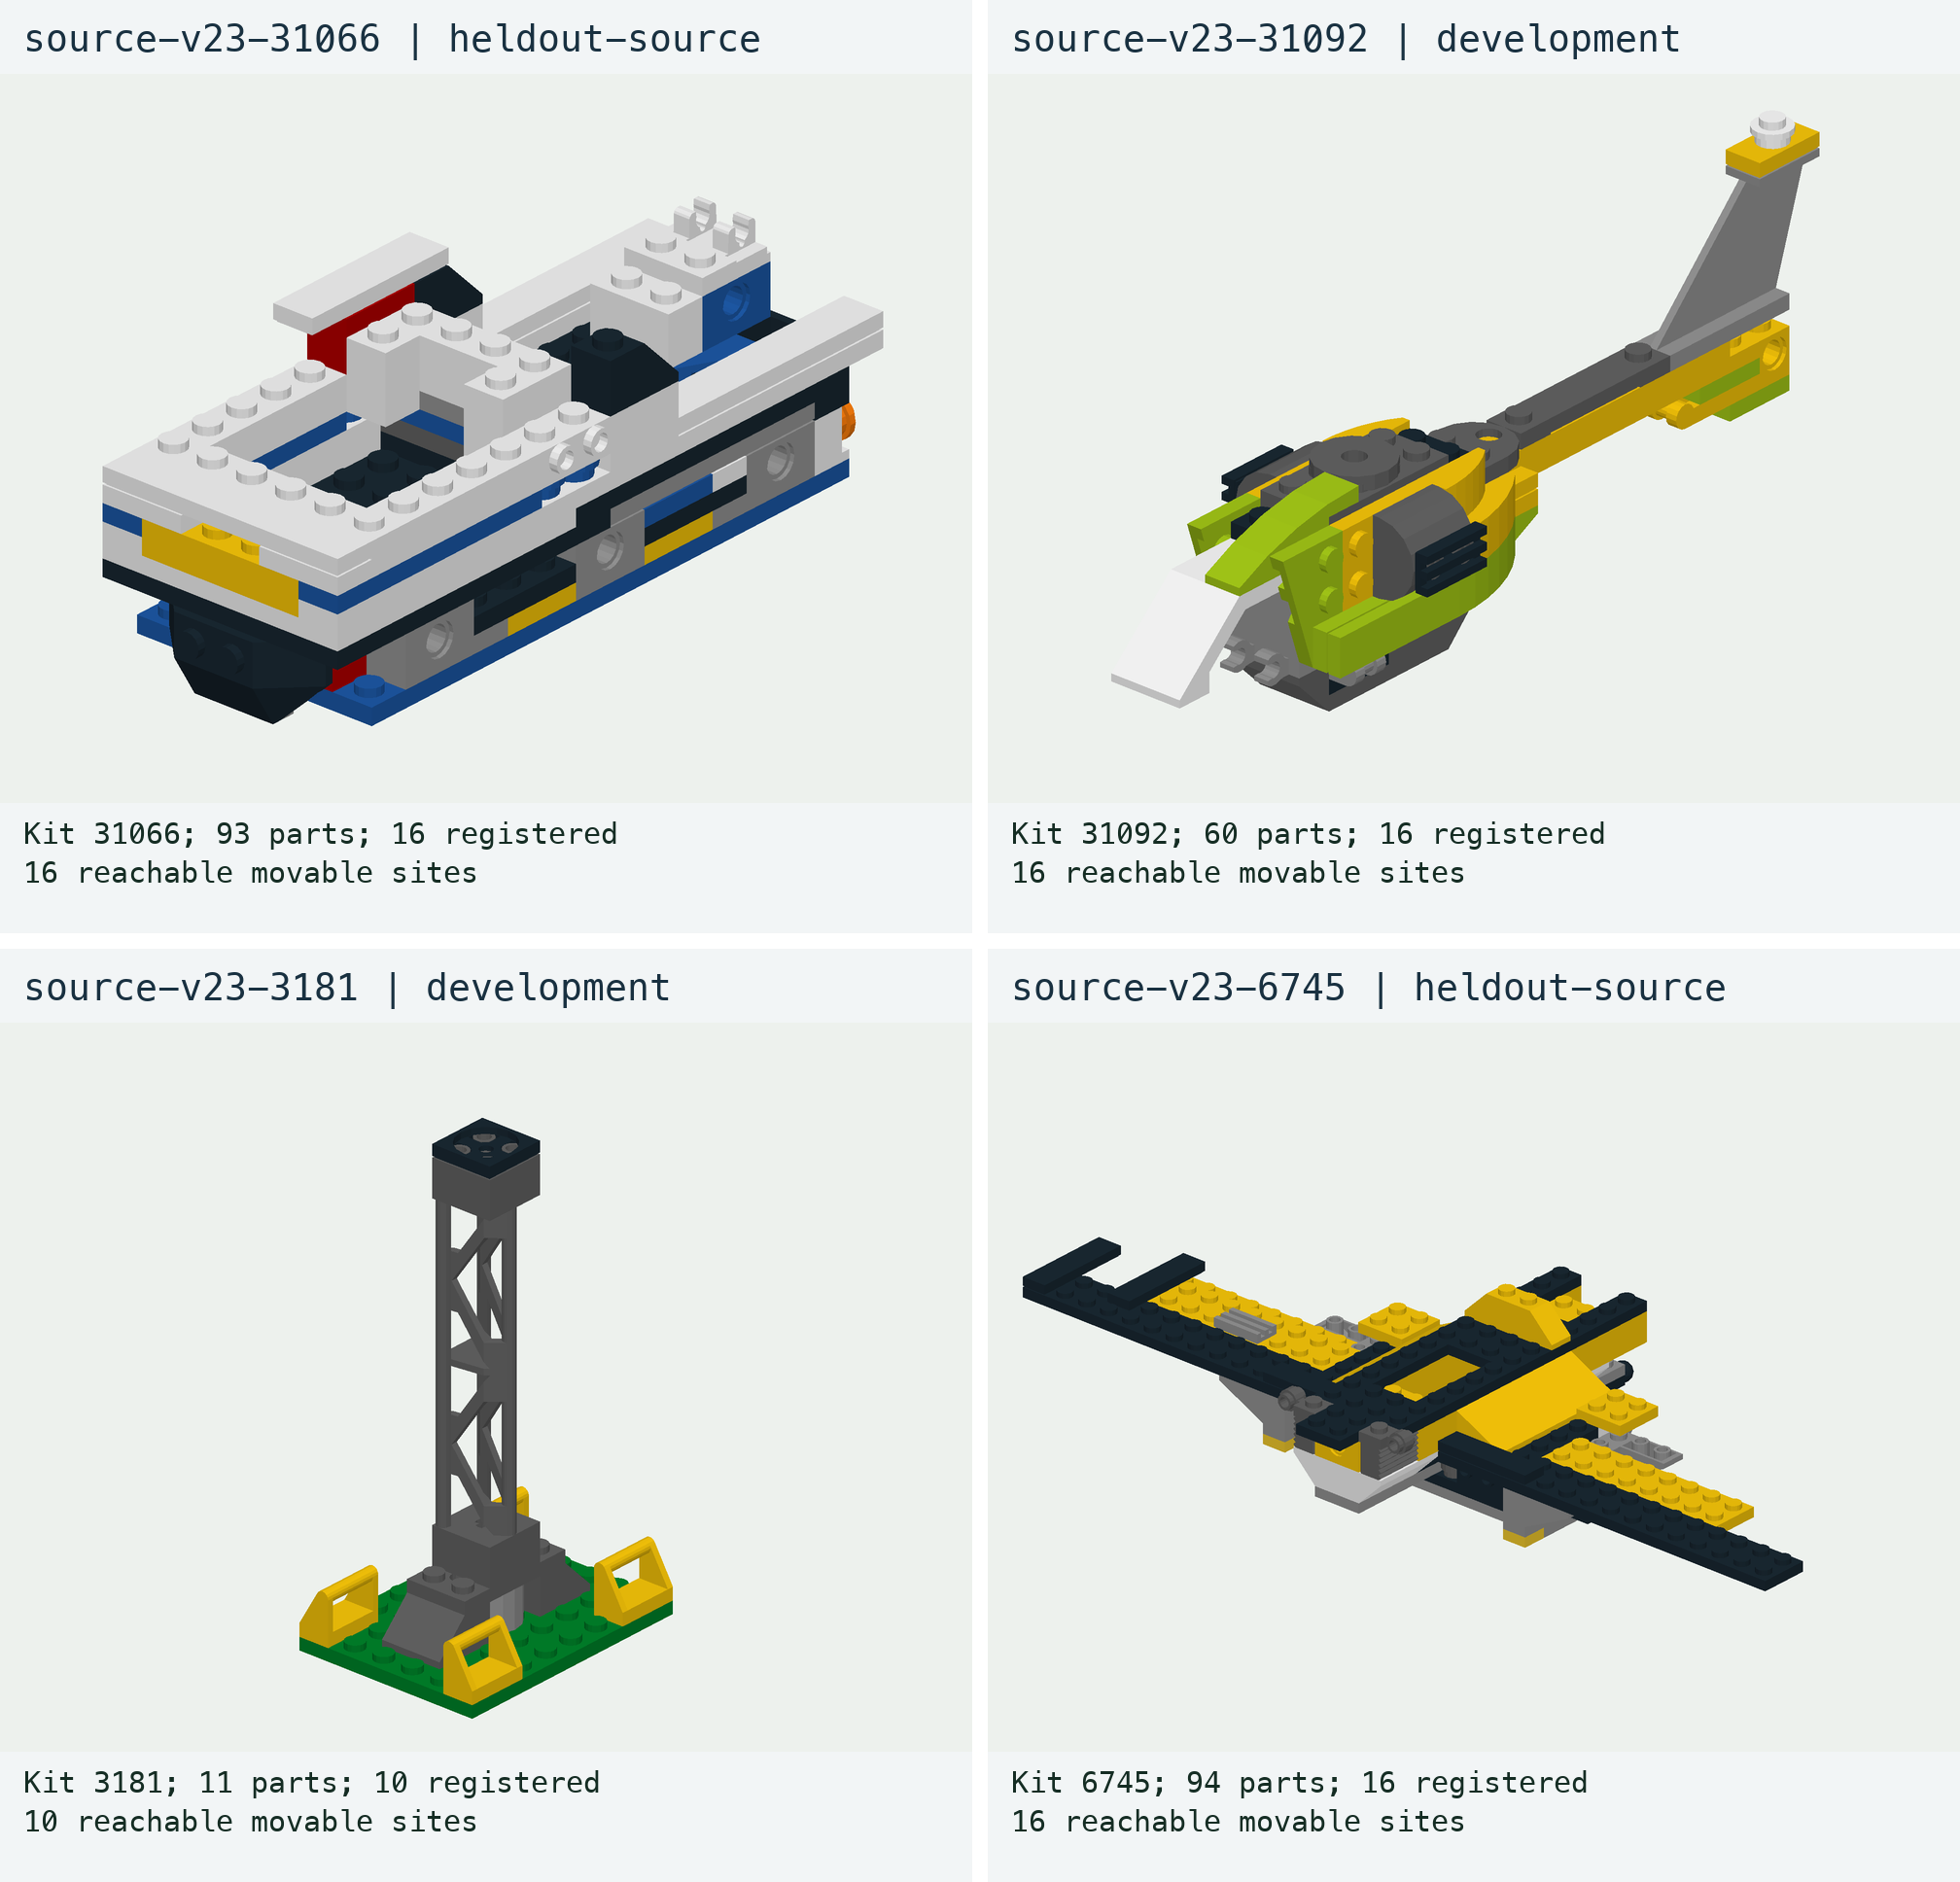
\includegraphics[width=.96\textwidth,height=.85\textheight,keepaspectratio]{figures/source-gallery-18.png}
\end{center}
\clearpage
\section*{Original-source gallery: assemblies 73--76}
\begin{center}
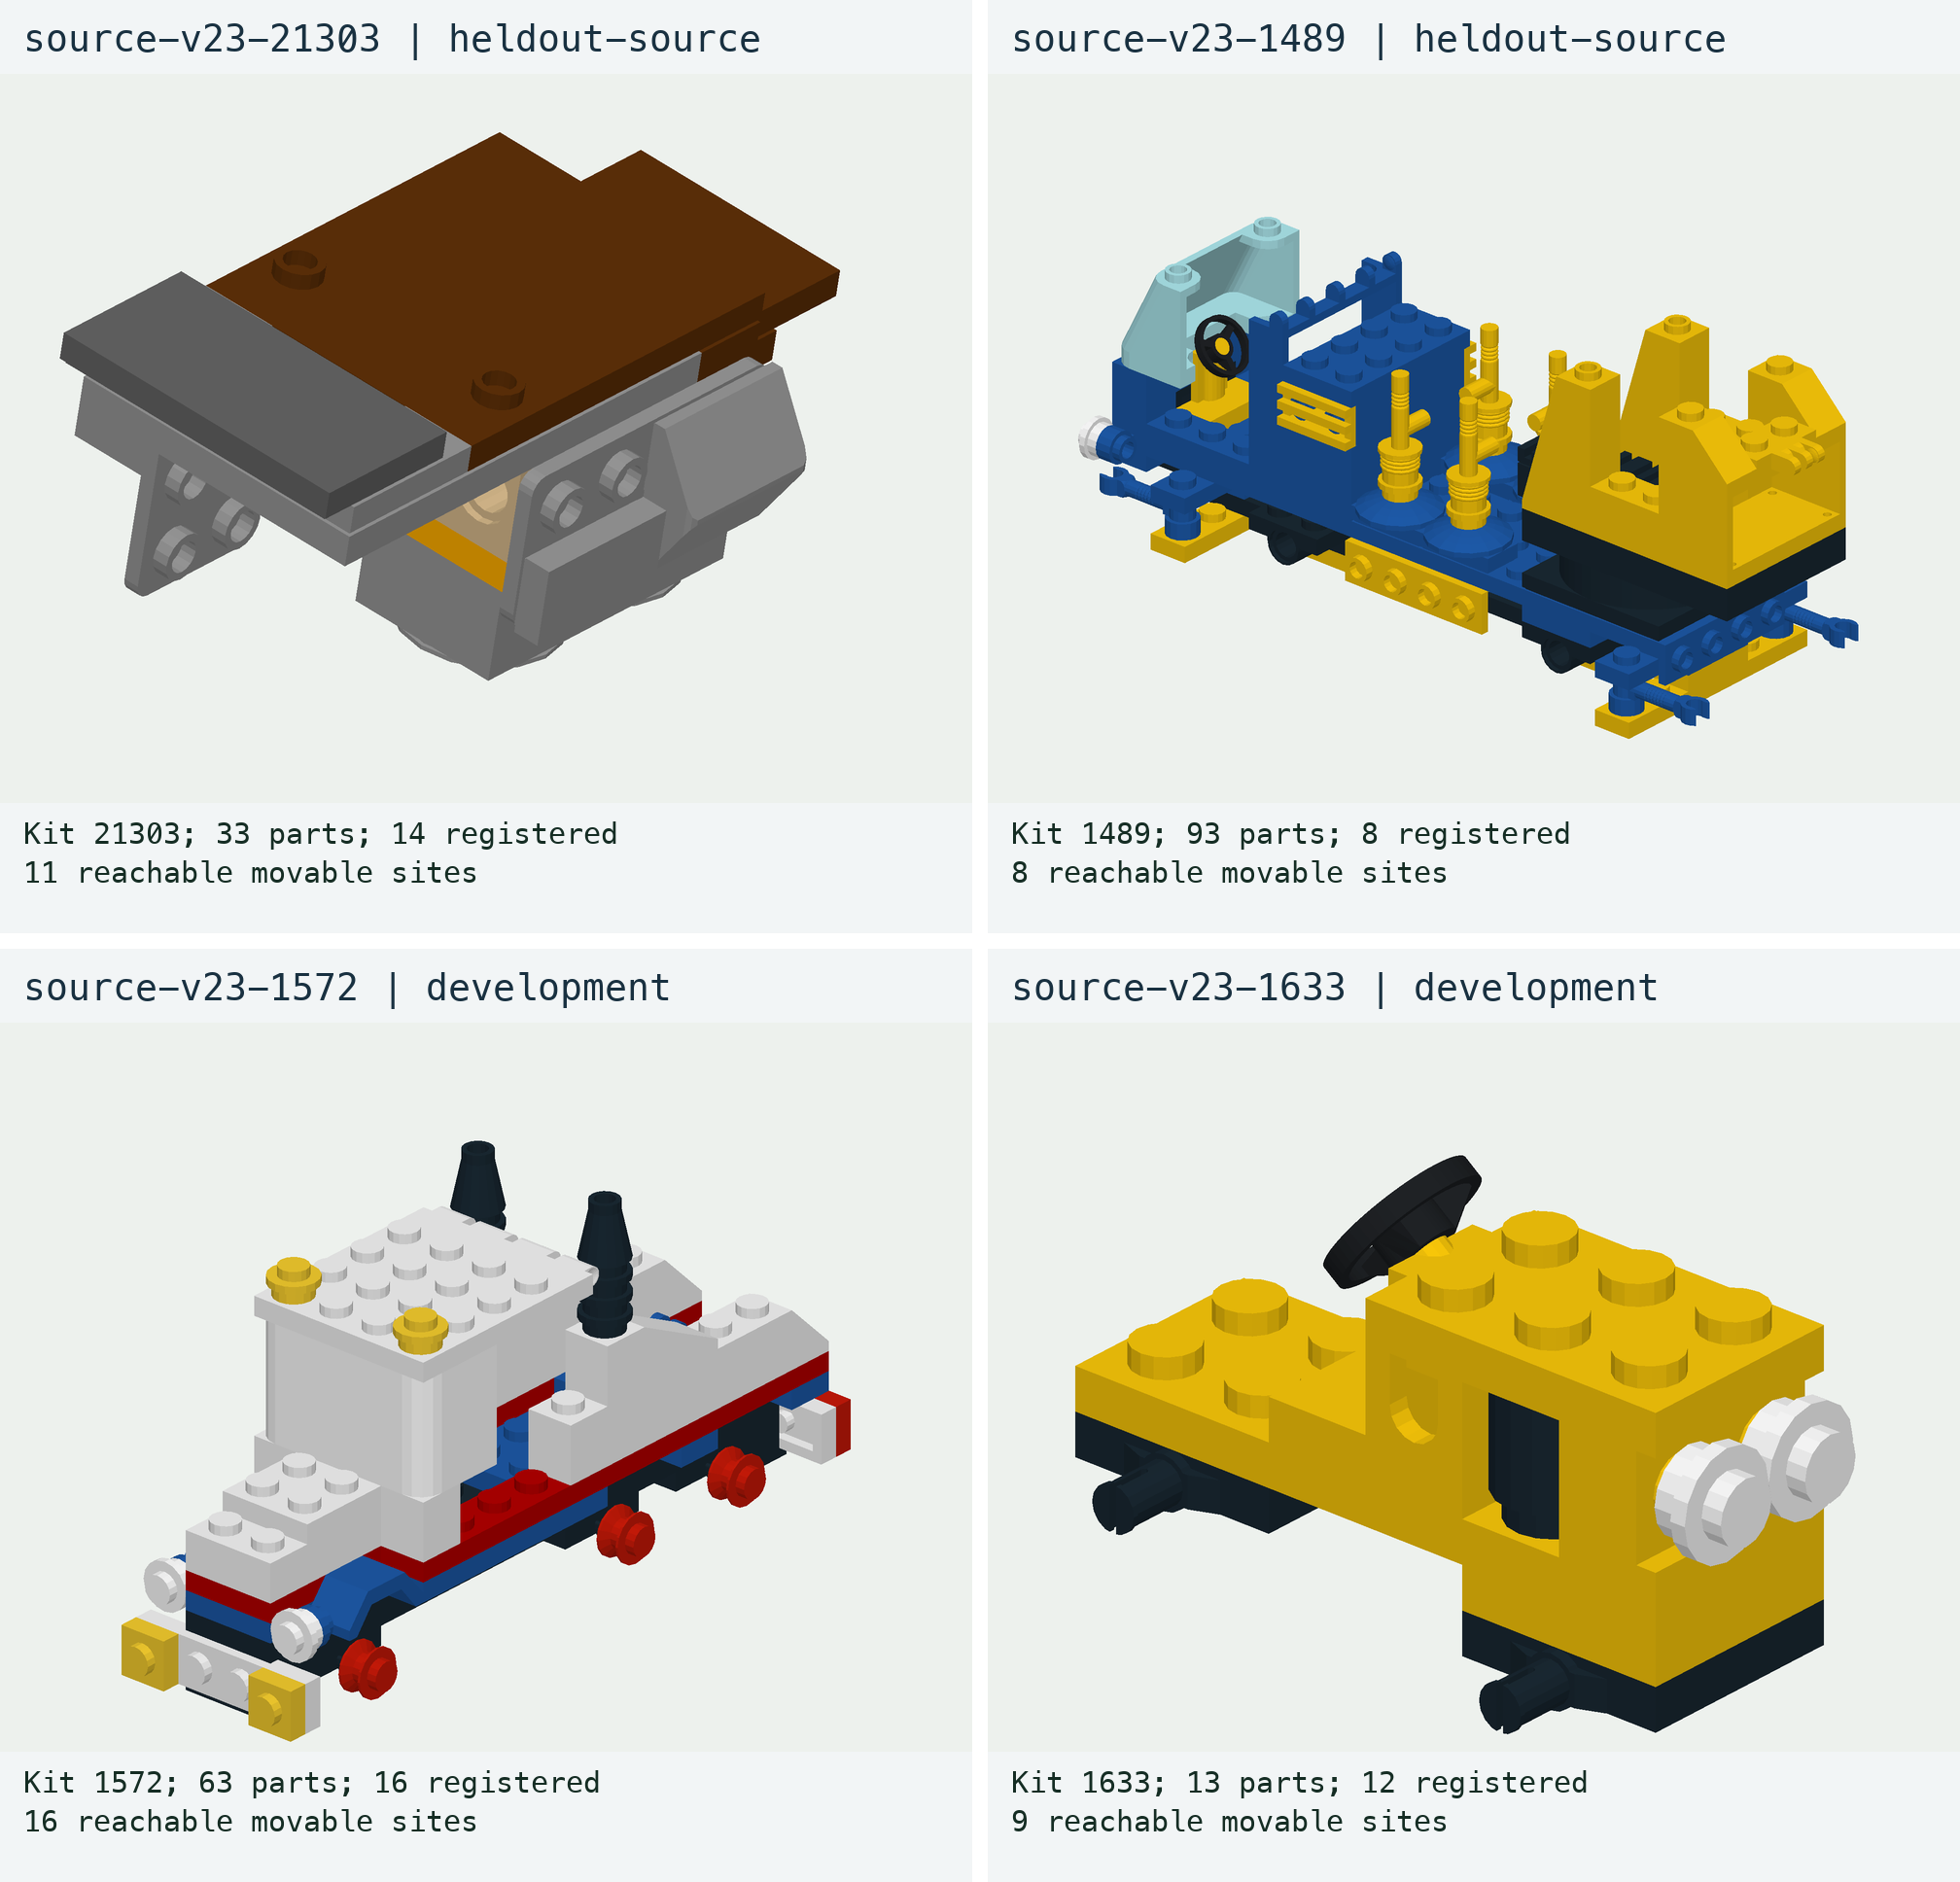
\includegraphics[width=.96\textwidth,height=.85\textheight,keepaspectratio]{figures/source-gallery-19.png}
\end{center}
\clearpage
\section*{Original-source gallery: assemblies 77--80}
\begin{center}
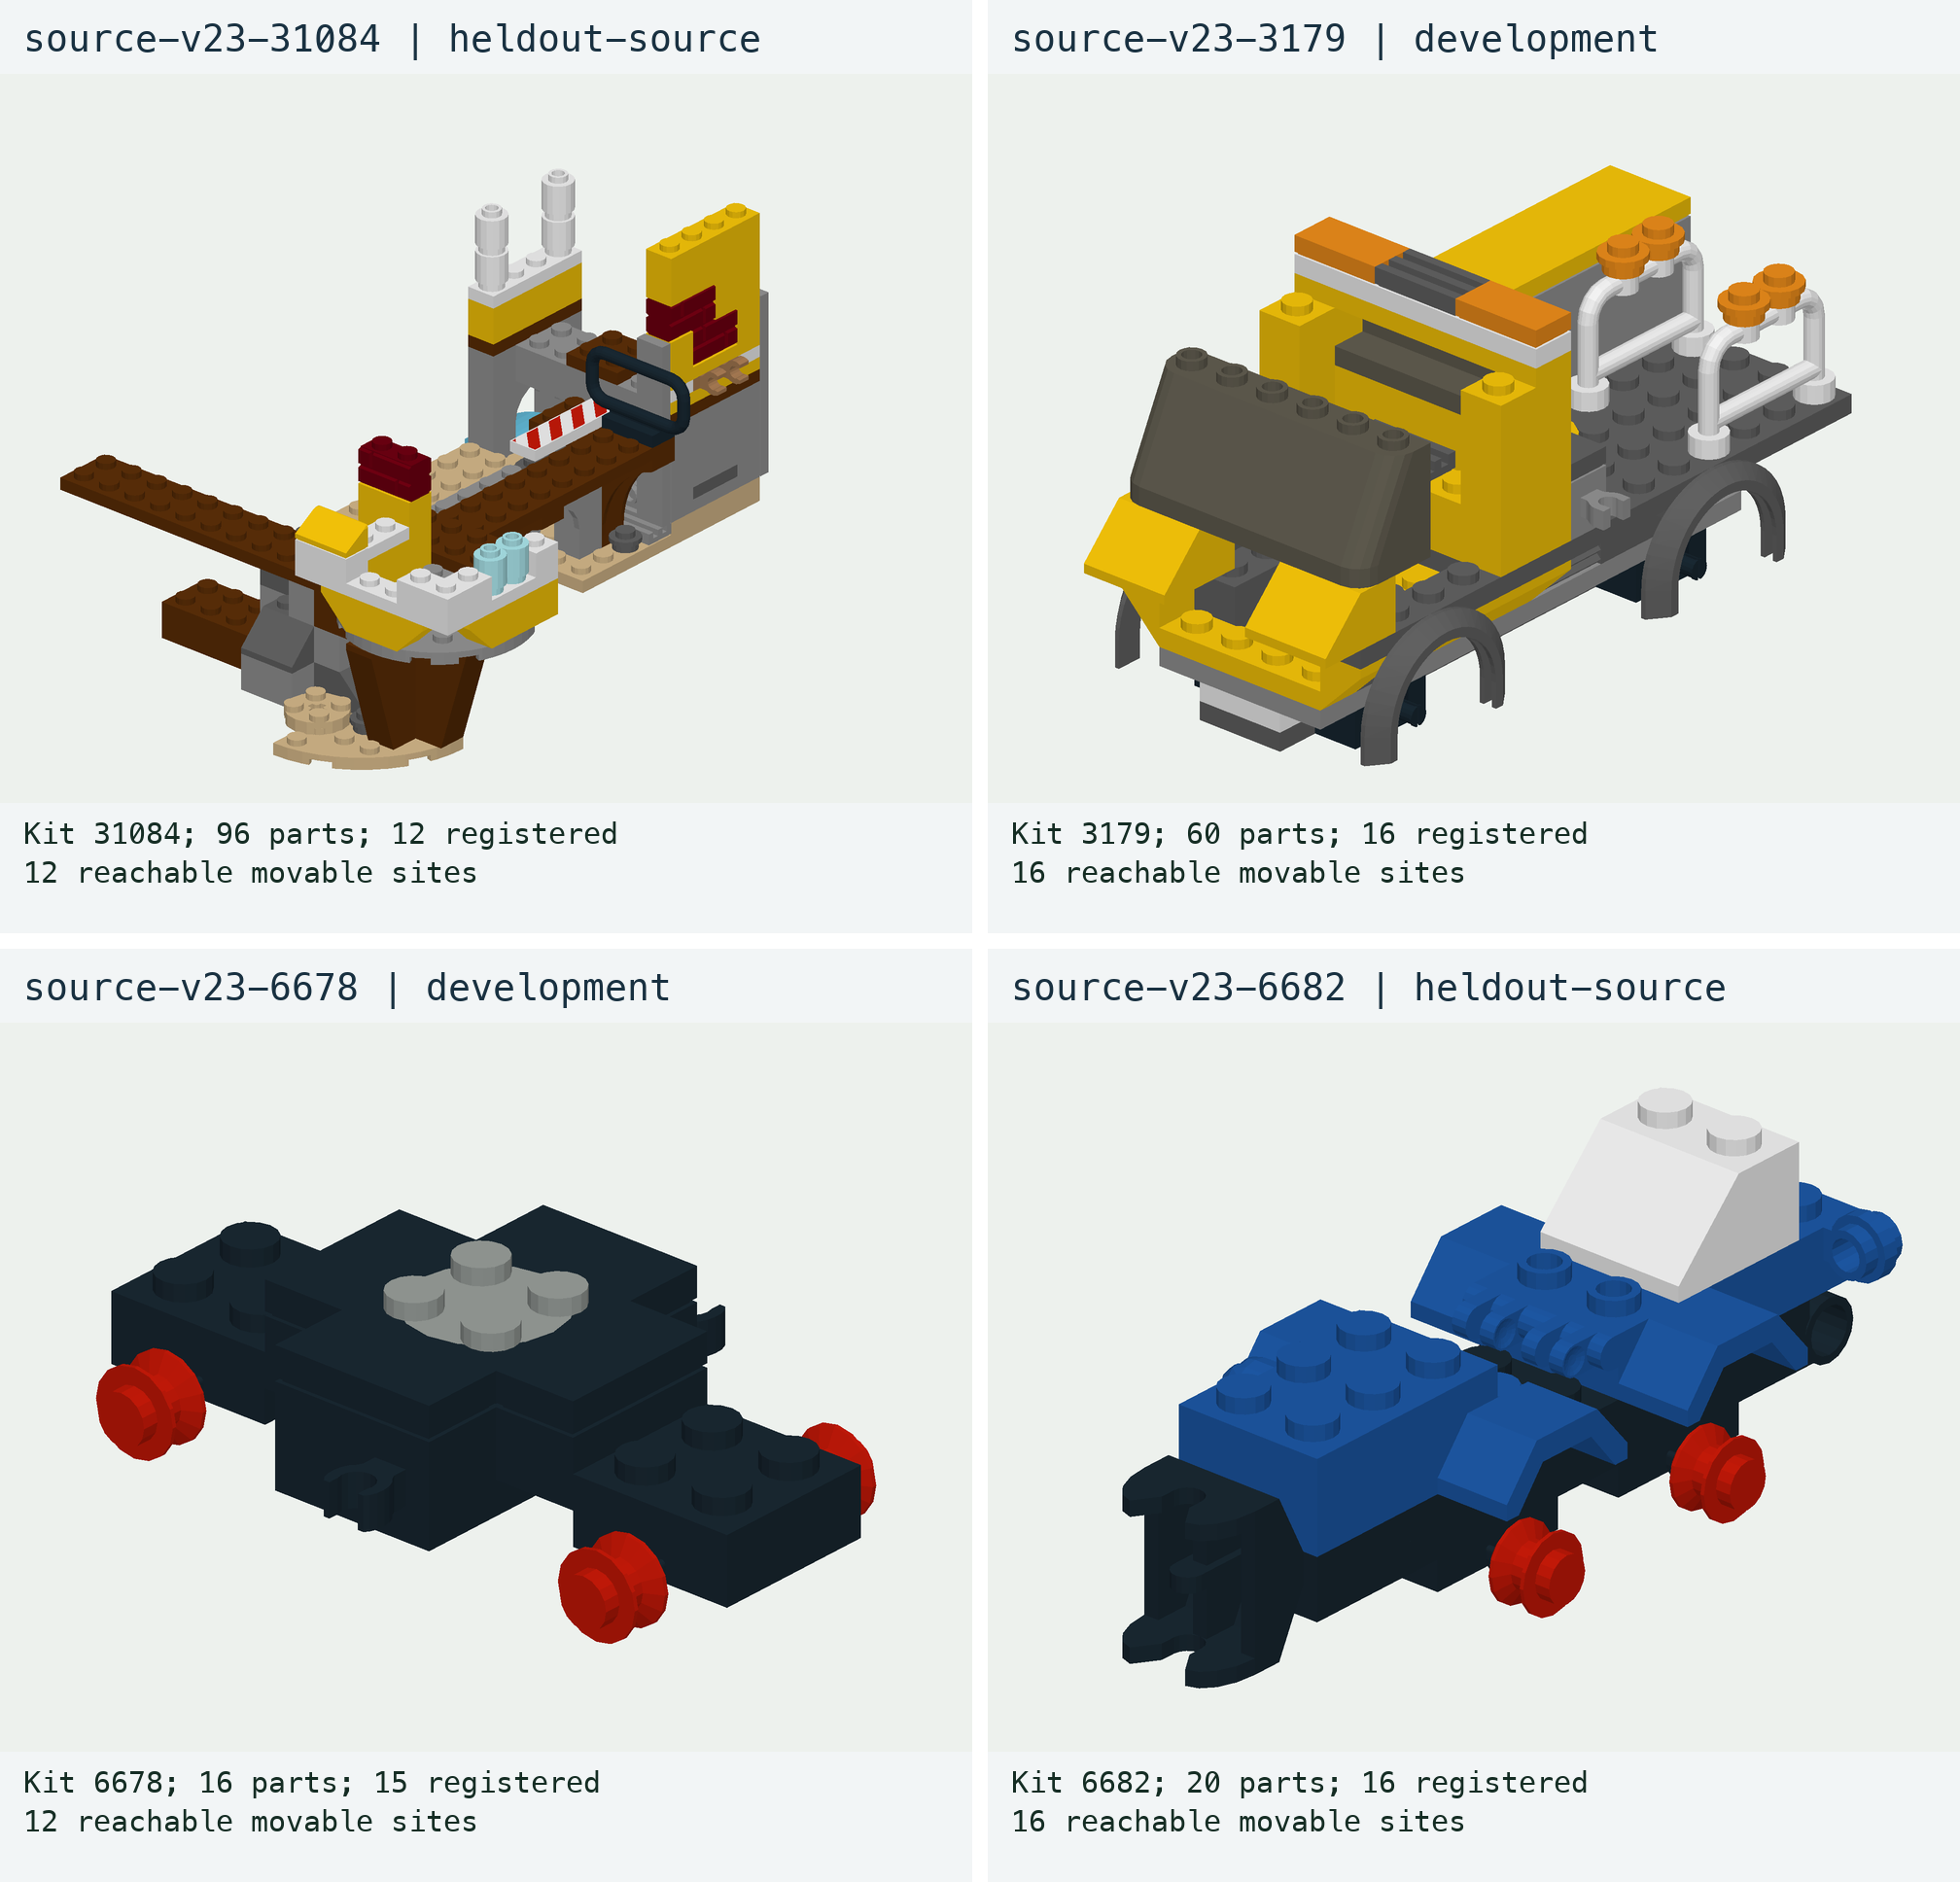
\includegraphics[width=.96\textwidth,height=.85\textheight,keepaspectratio]{figures/source-gallery-20.png}
\end{center}
\clearpage
\section*{Original-source gallery: assemblies 81--84}
\begin{center}
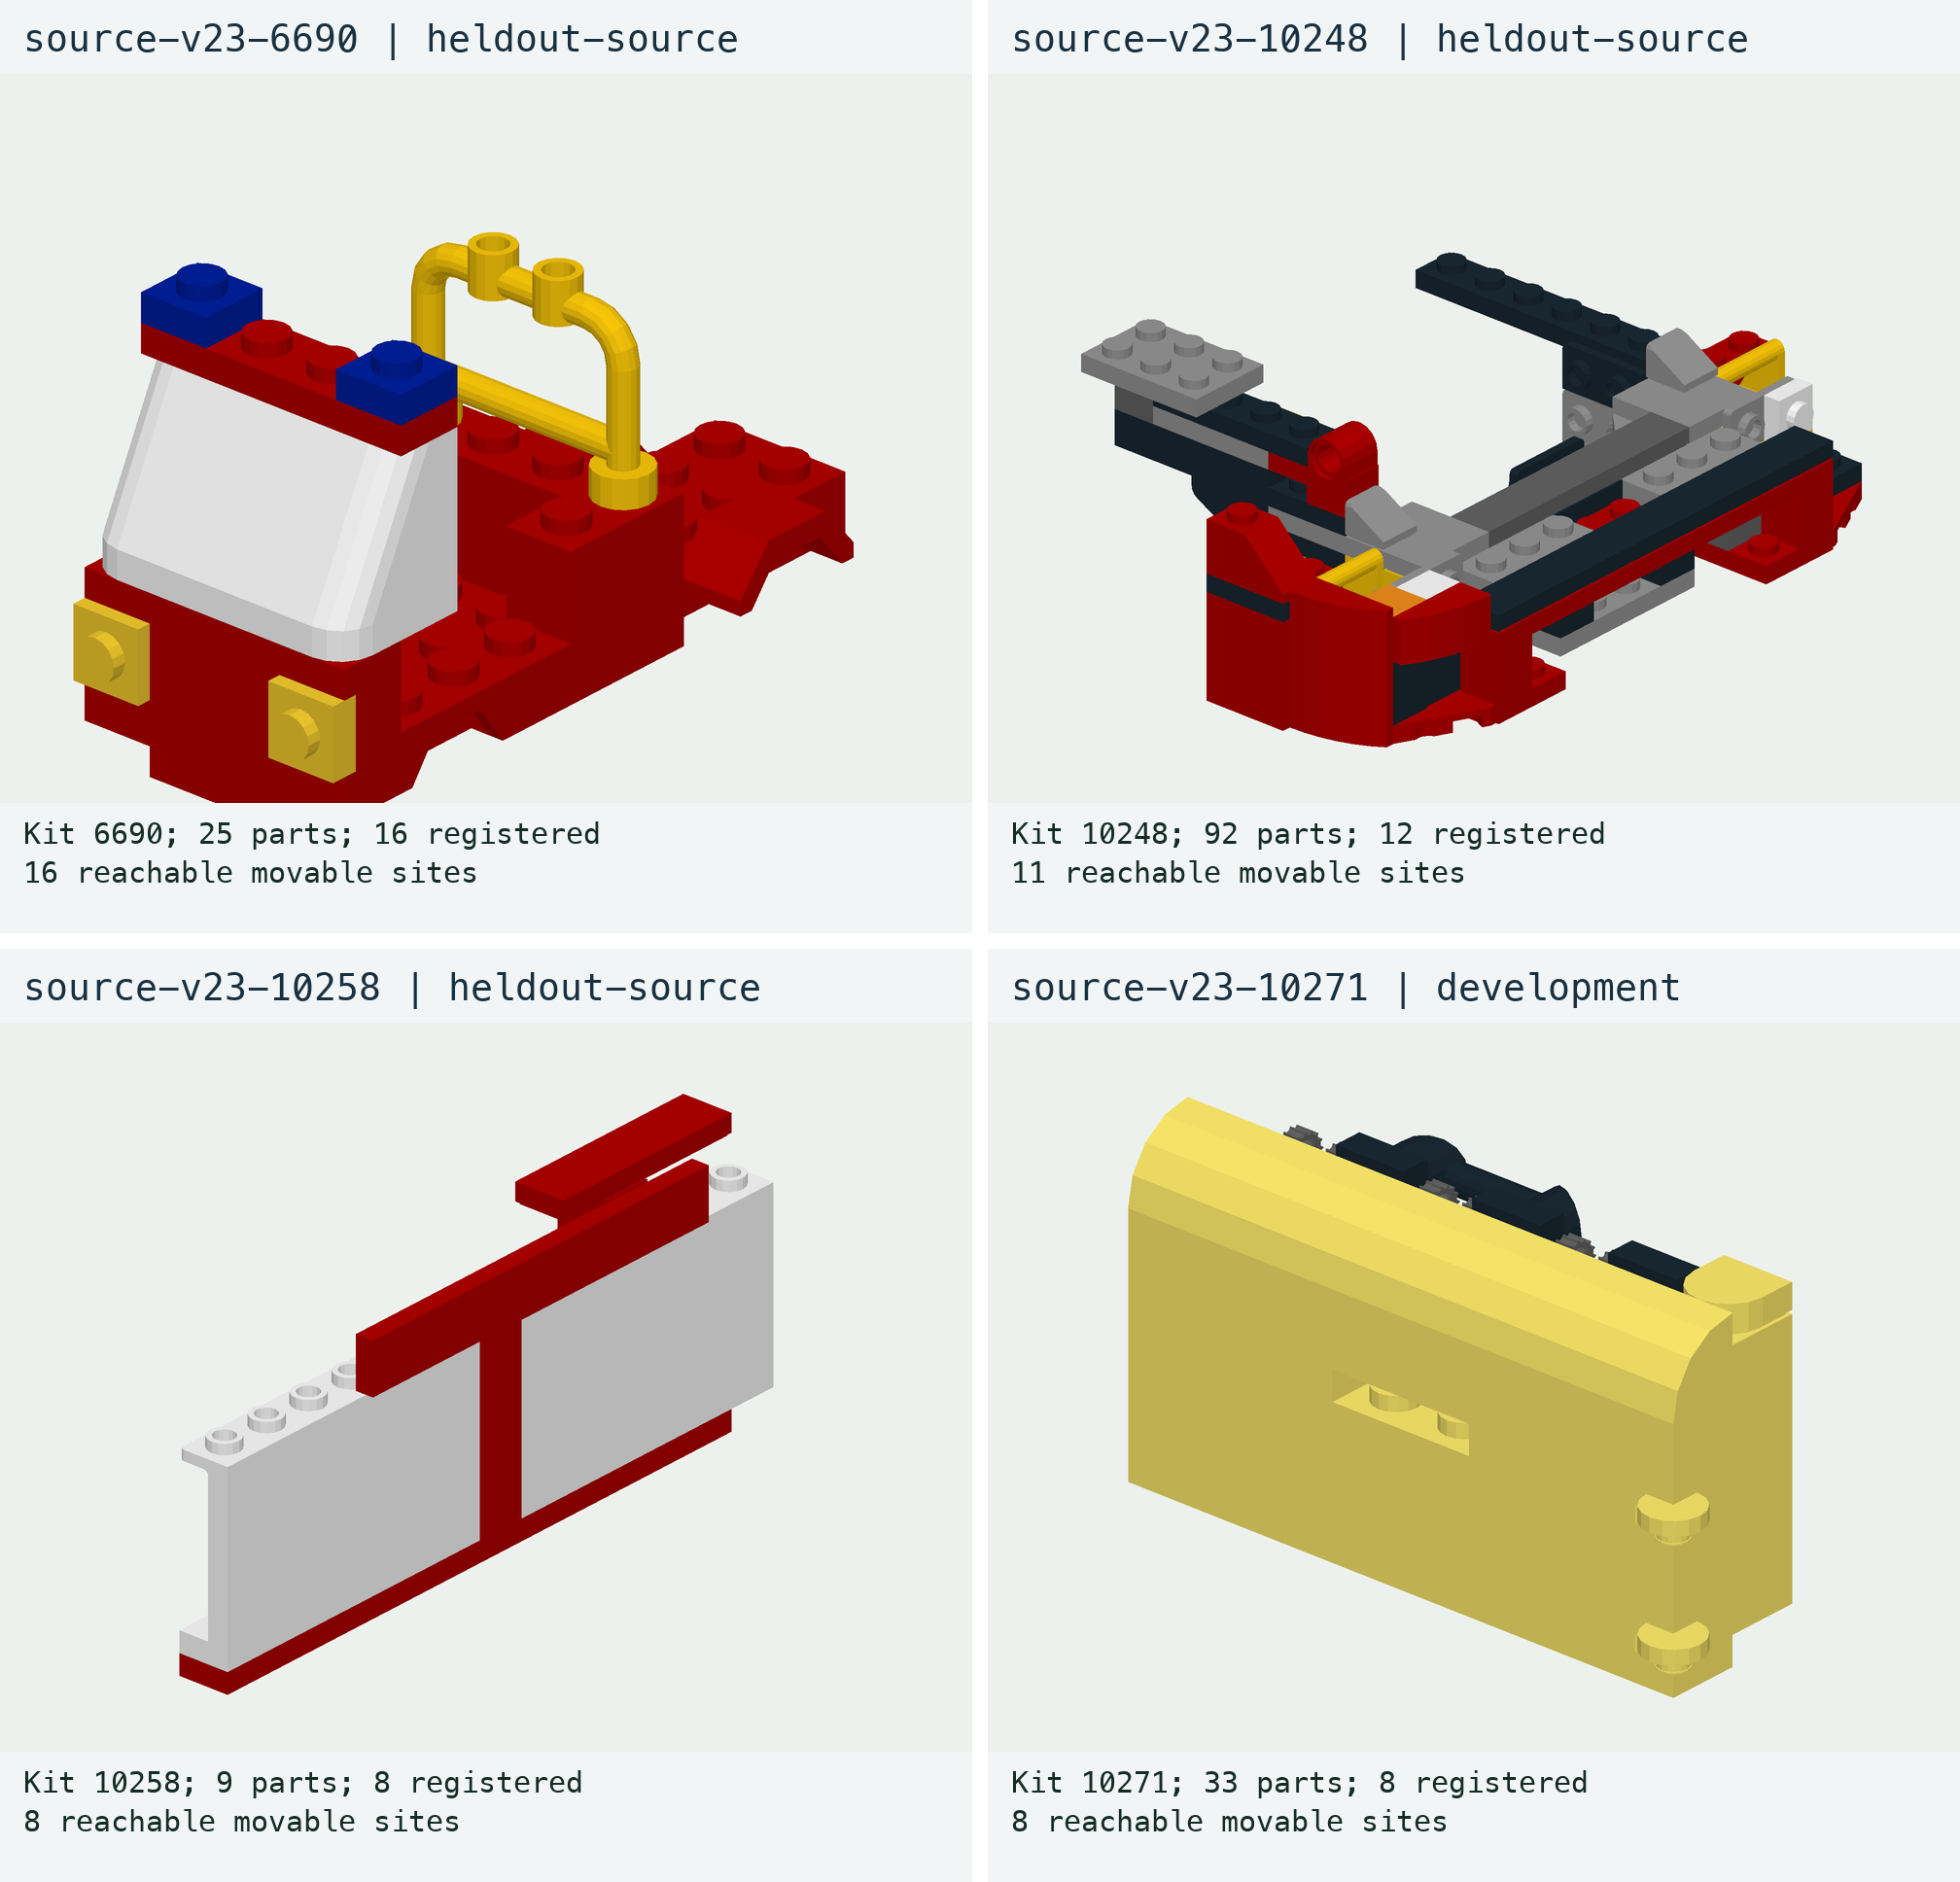
\includegraphics[width=.96\textwidth,height=.85\textheight,keepaspectratio]{figures/source-gallery-21.png}
\end{center}
\clearpage
\section*{Original-source gallery: assemblies 85--88}
\begin{center}
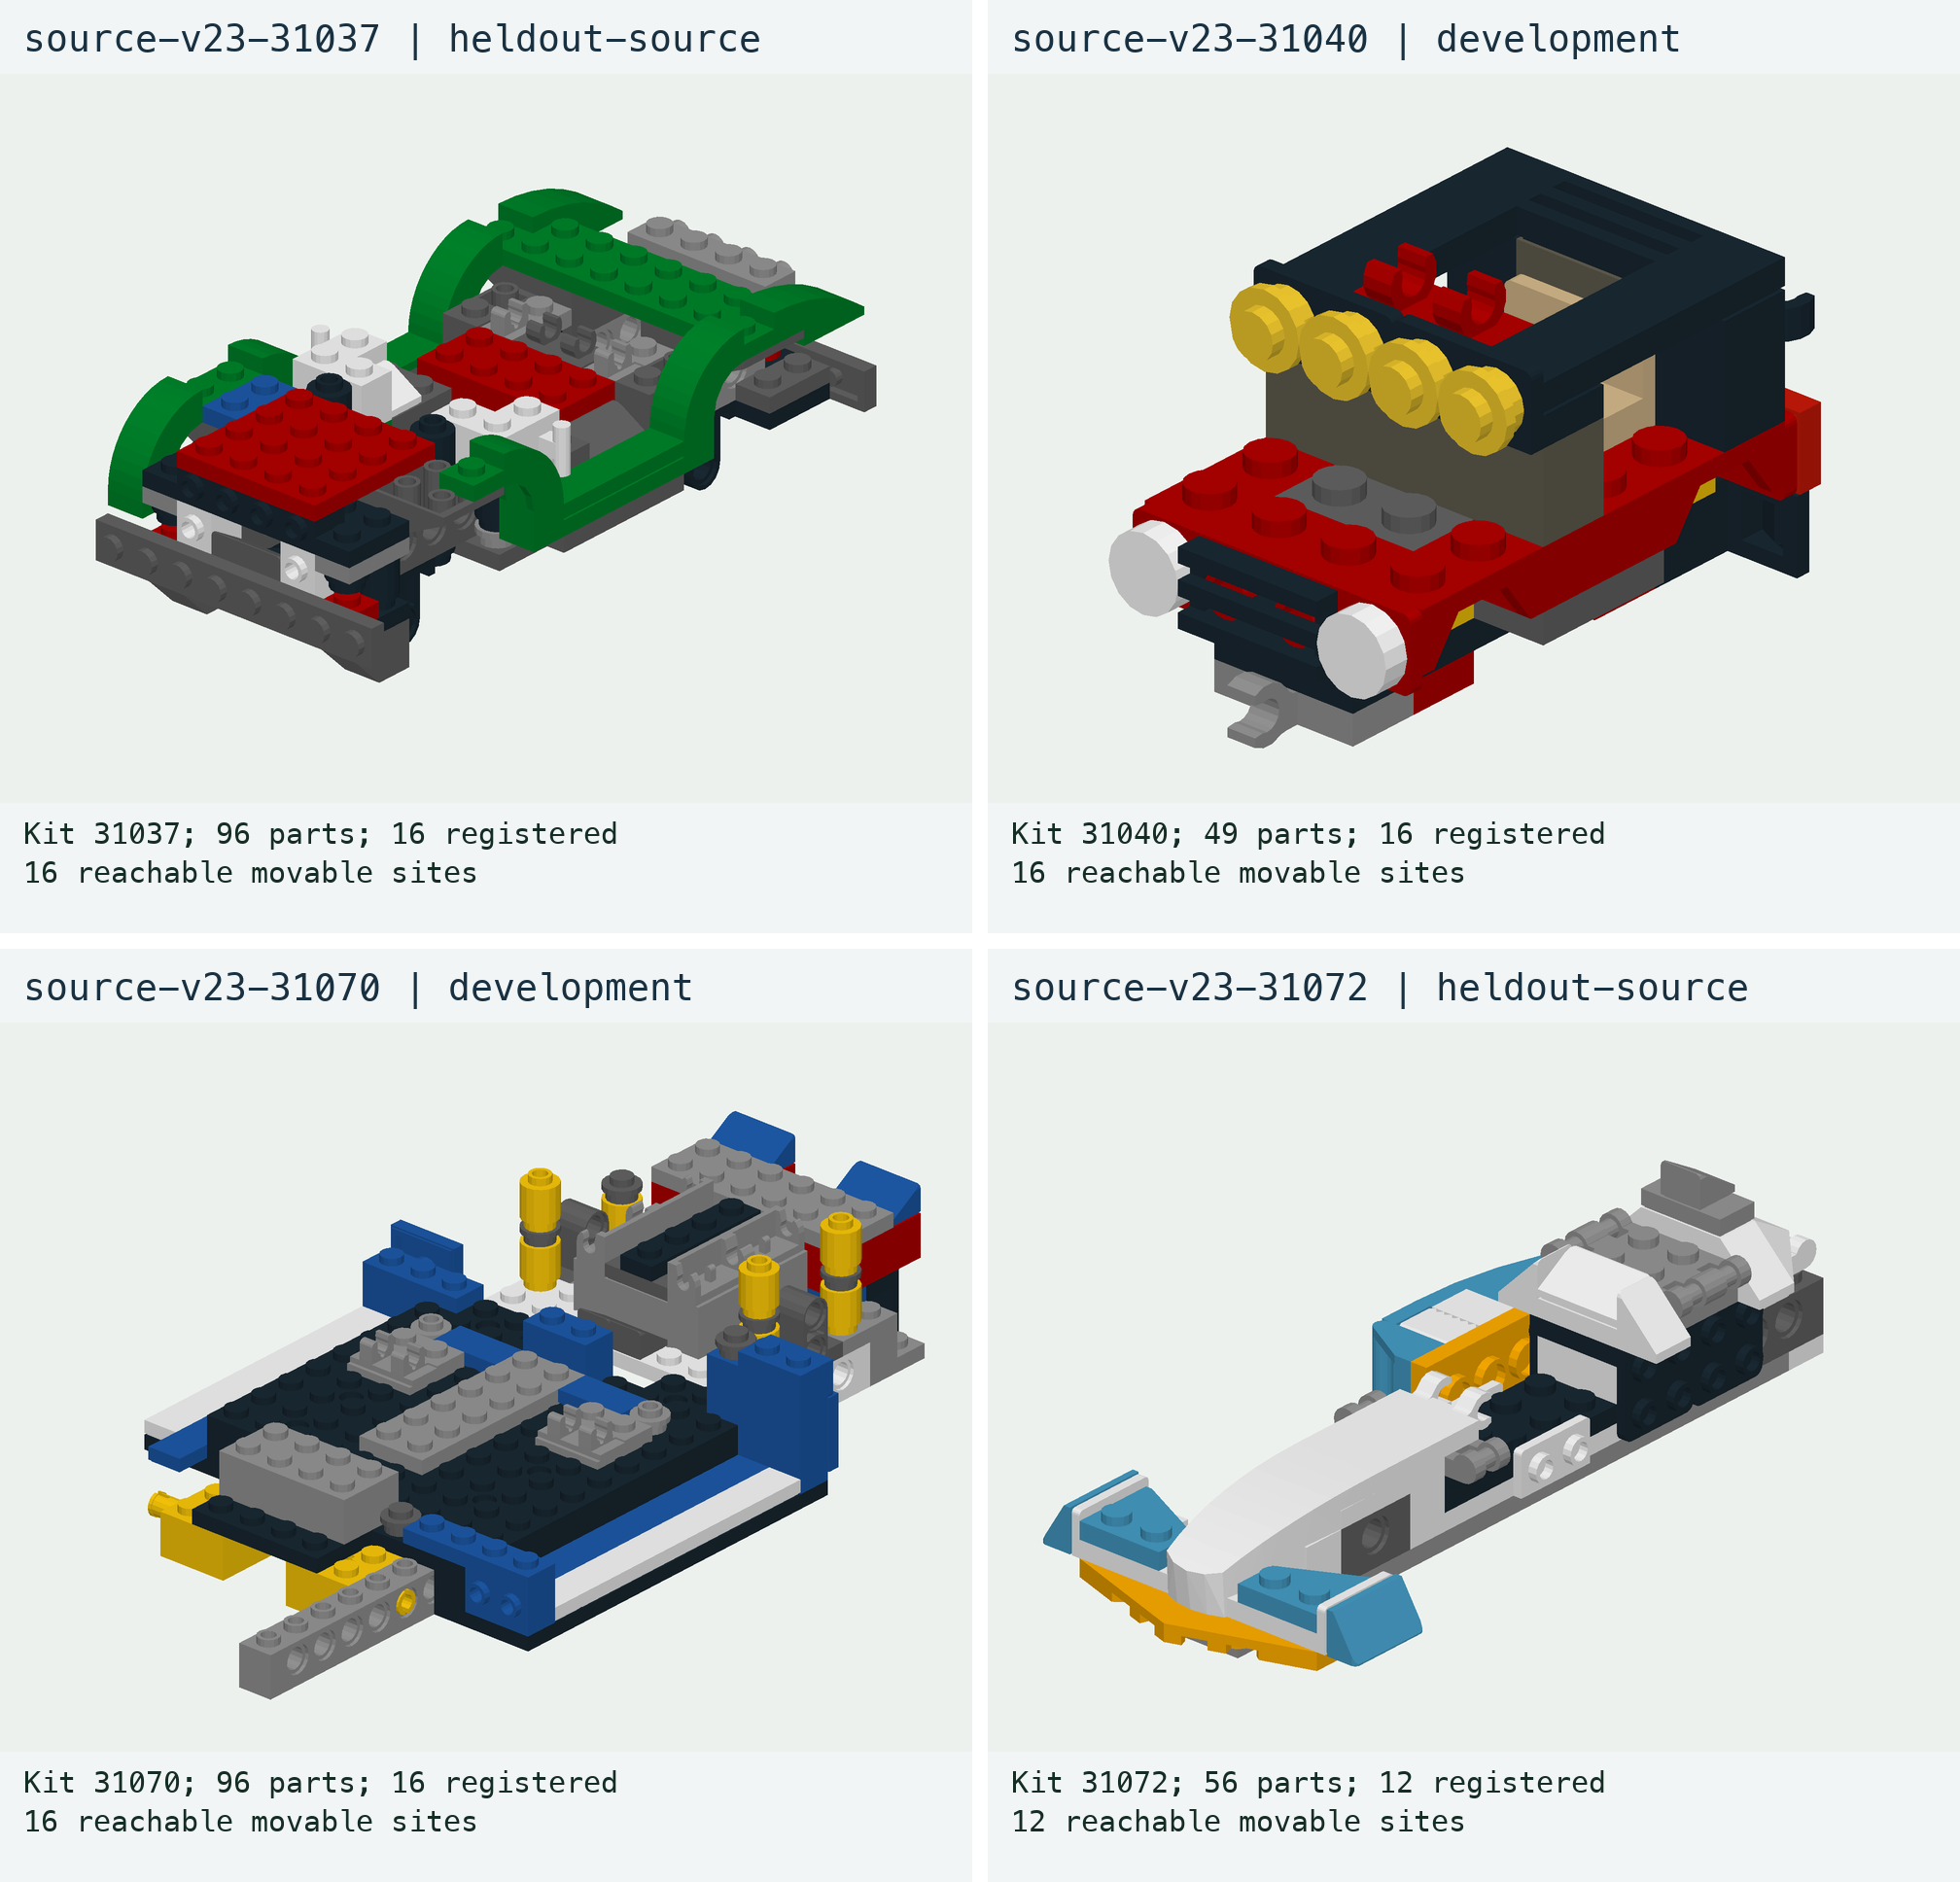
\includegraphics[width=.96\textwidth,height=.85\textheight,keepaspectratio]{figures/source-gallery-22.png}
\end{center}
\clearpage
\section*{Original-source gallery: assemblies 89--92}
\begin{center}
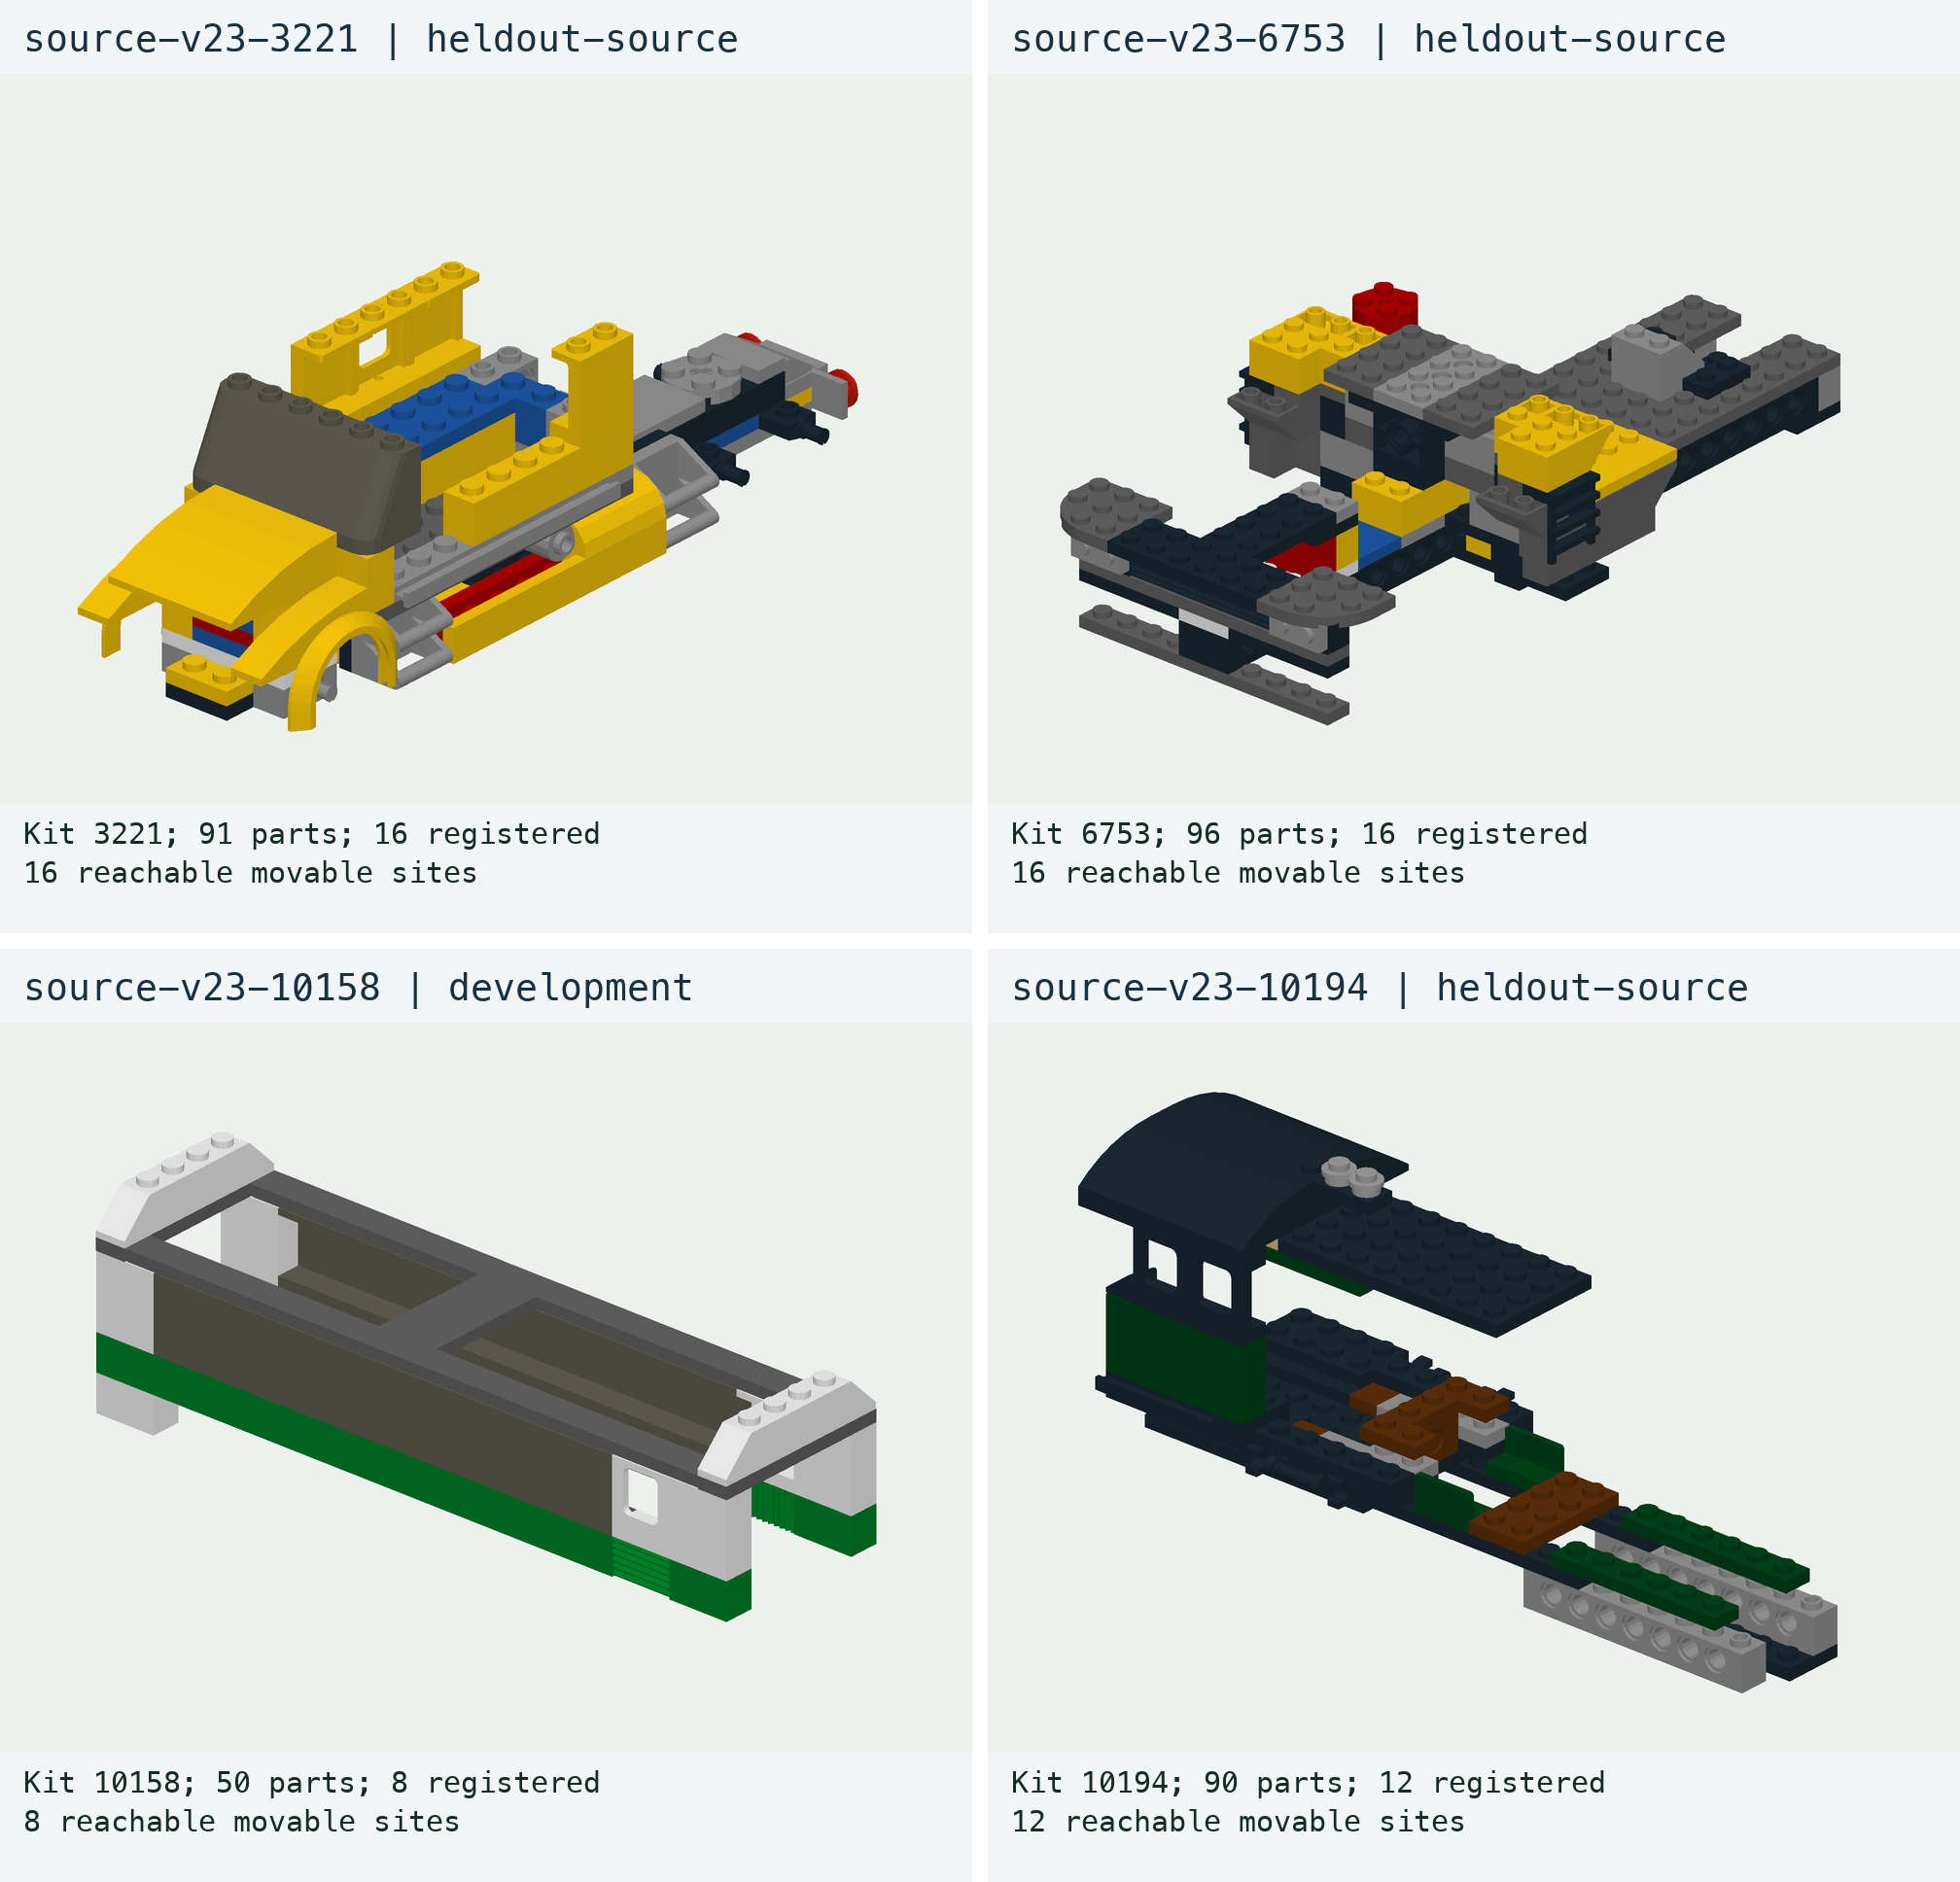
\includegraphics[width=.96\textwidth,height=.85\textheight,keepaspectratio]{figures/source-gallery-23.png}
\end{center}
\clearpage
\section*{Original-source gallery: assemblies 93--96}
\begin{center}
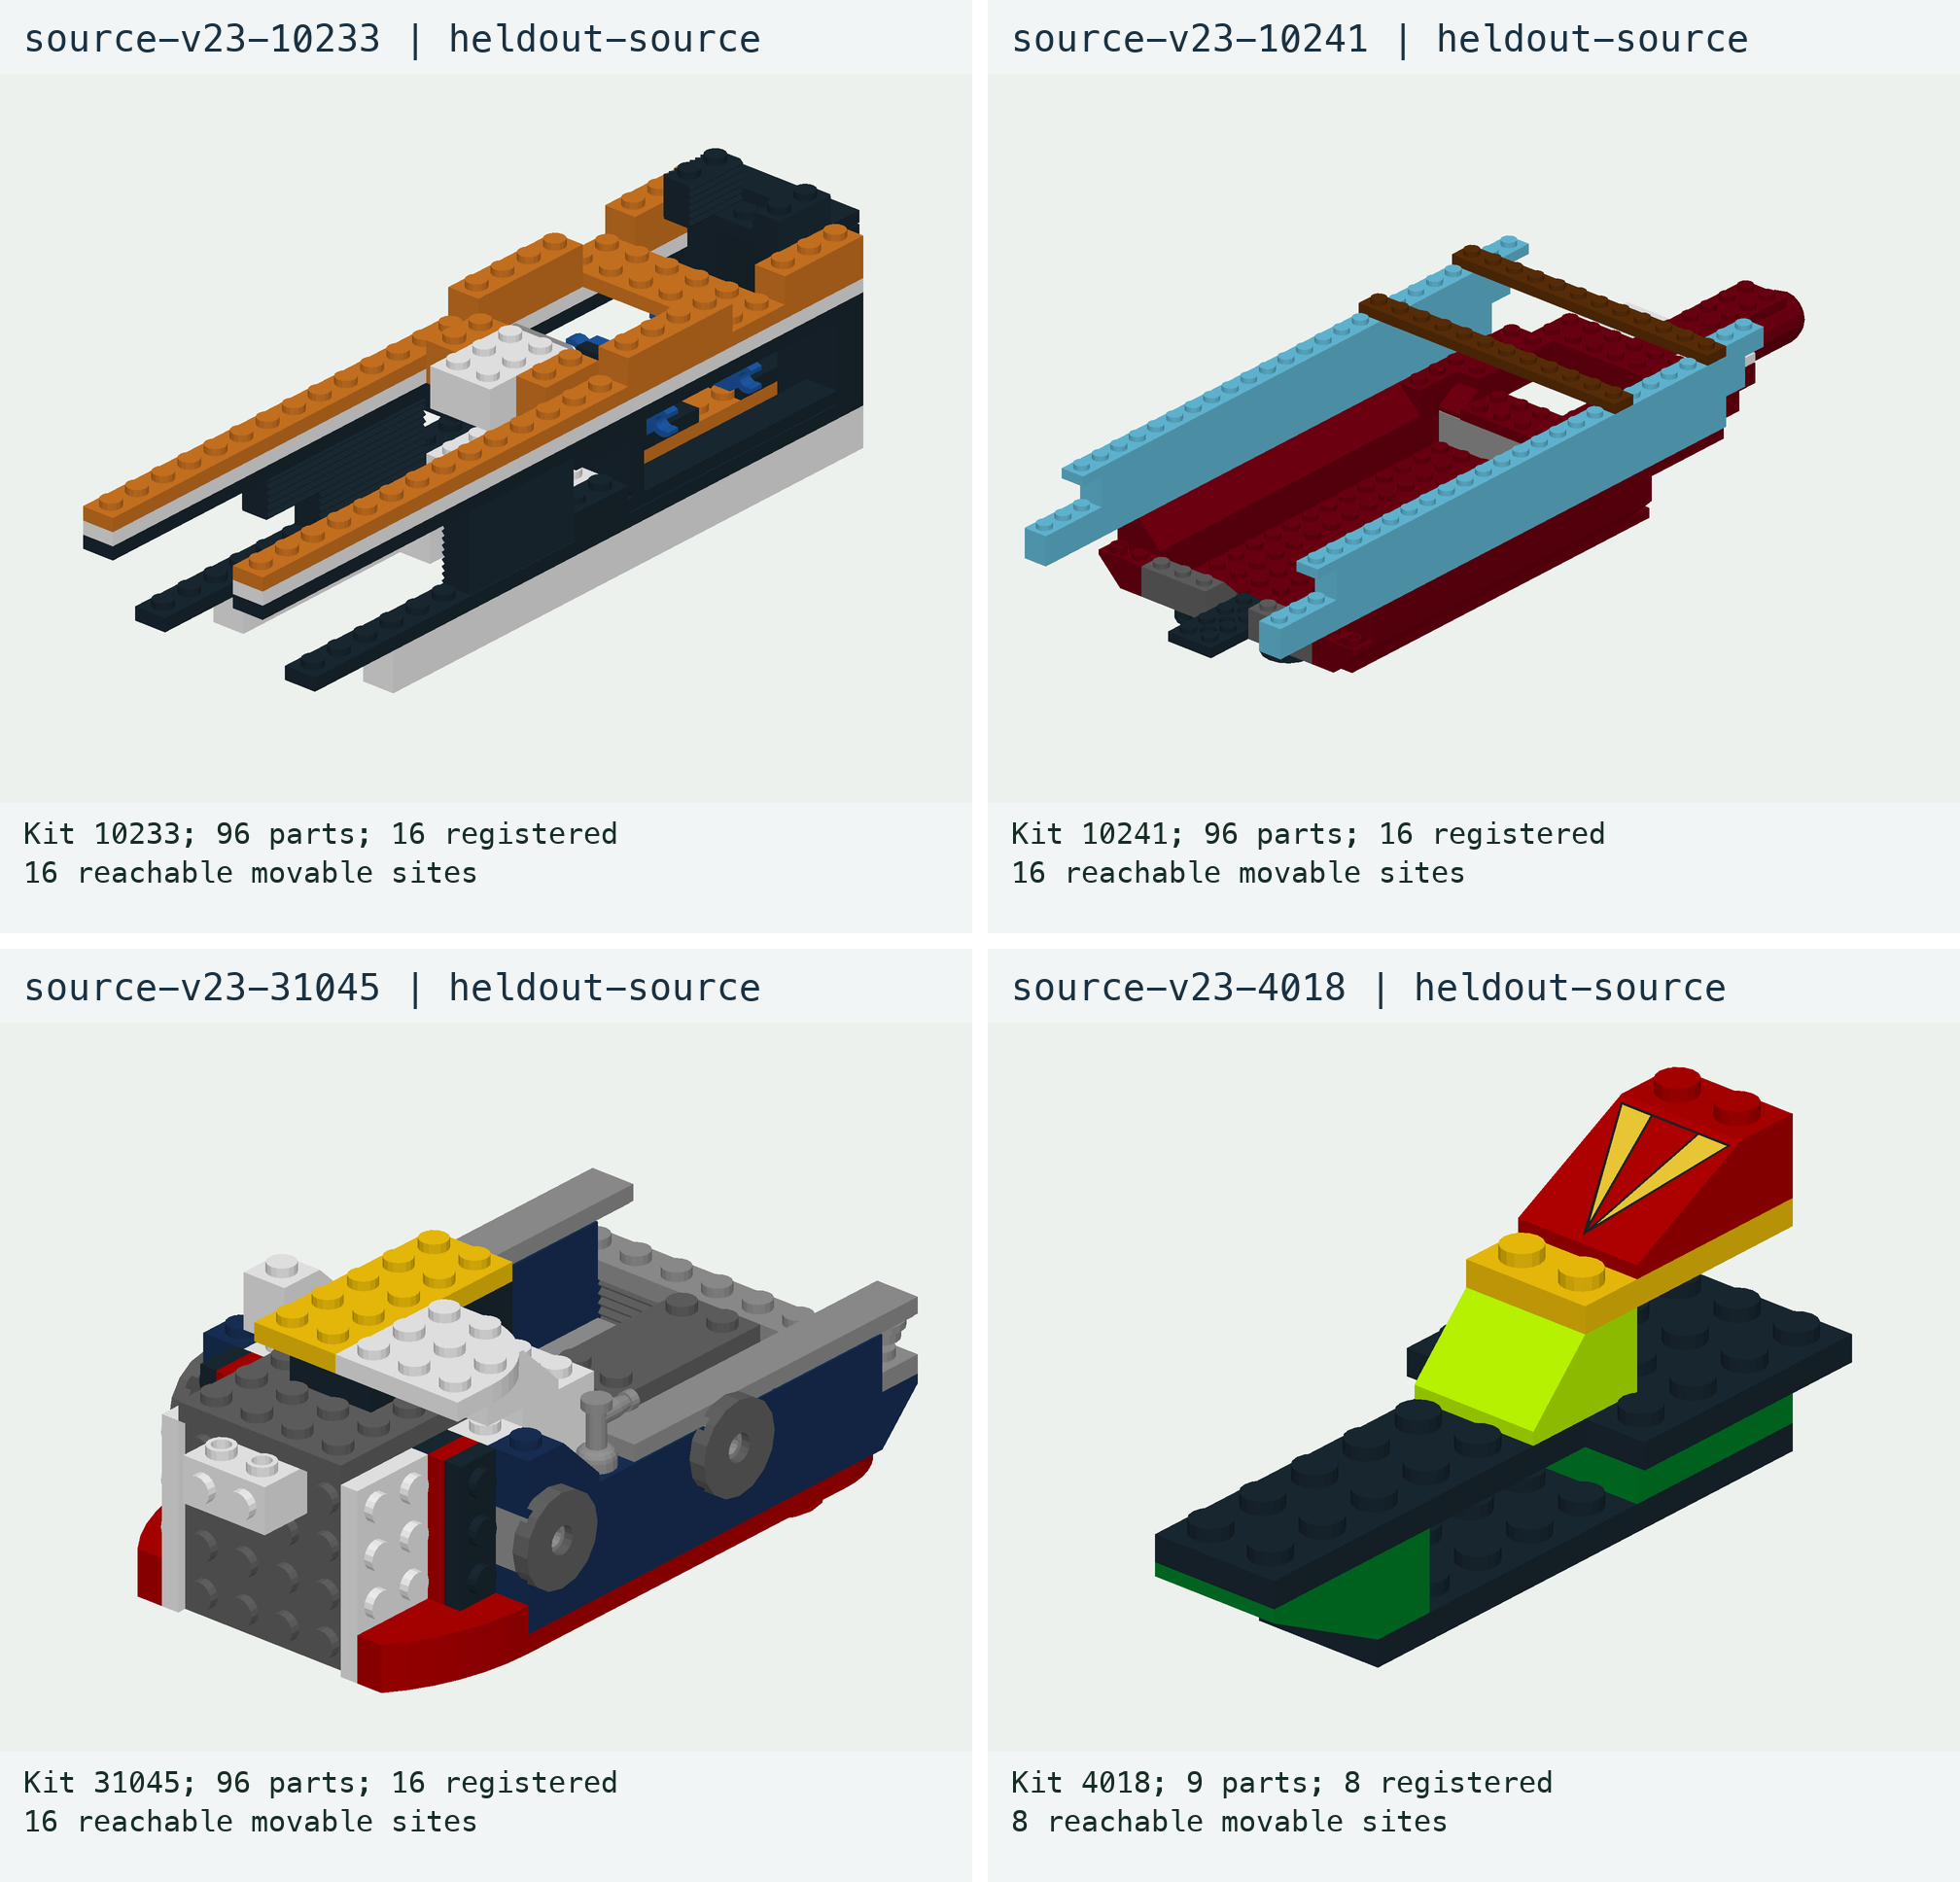
\includegraphics[width=.96\textwidth,height=.85\textheight,keepaspectratio]{figures/source-gallery-24.png}
\end{center}
\clearpage
\section*{Original-source gallery: assemblies 97--98}
\begin{center}
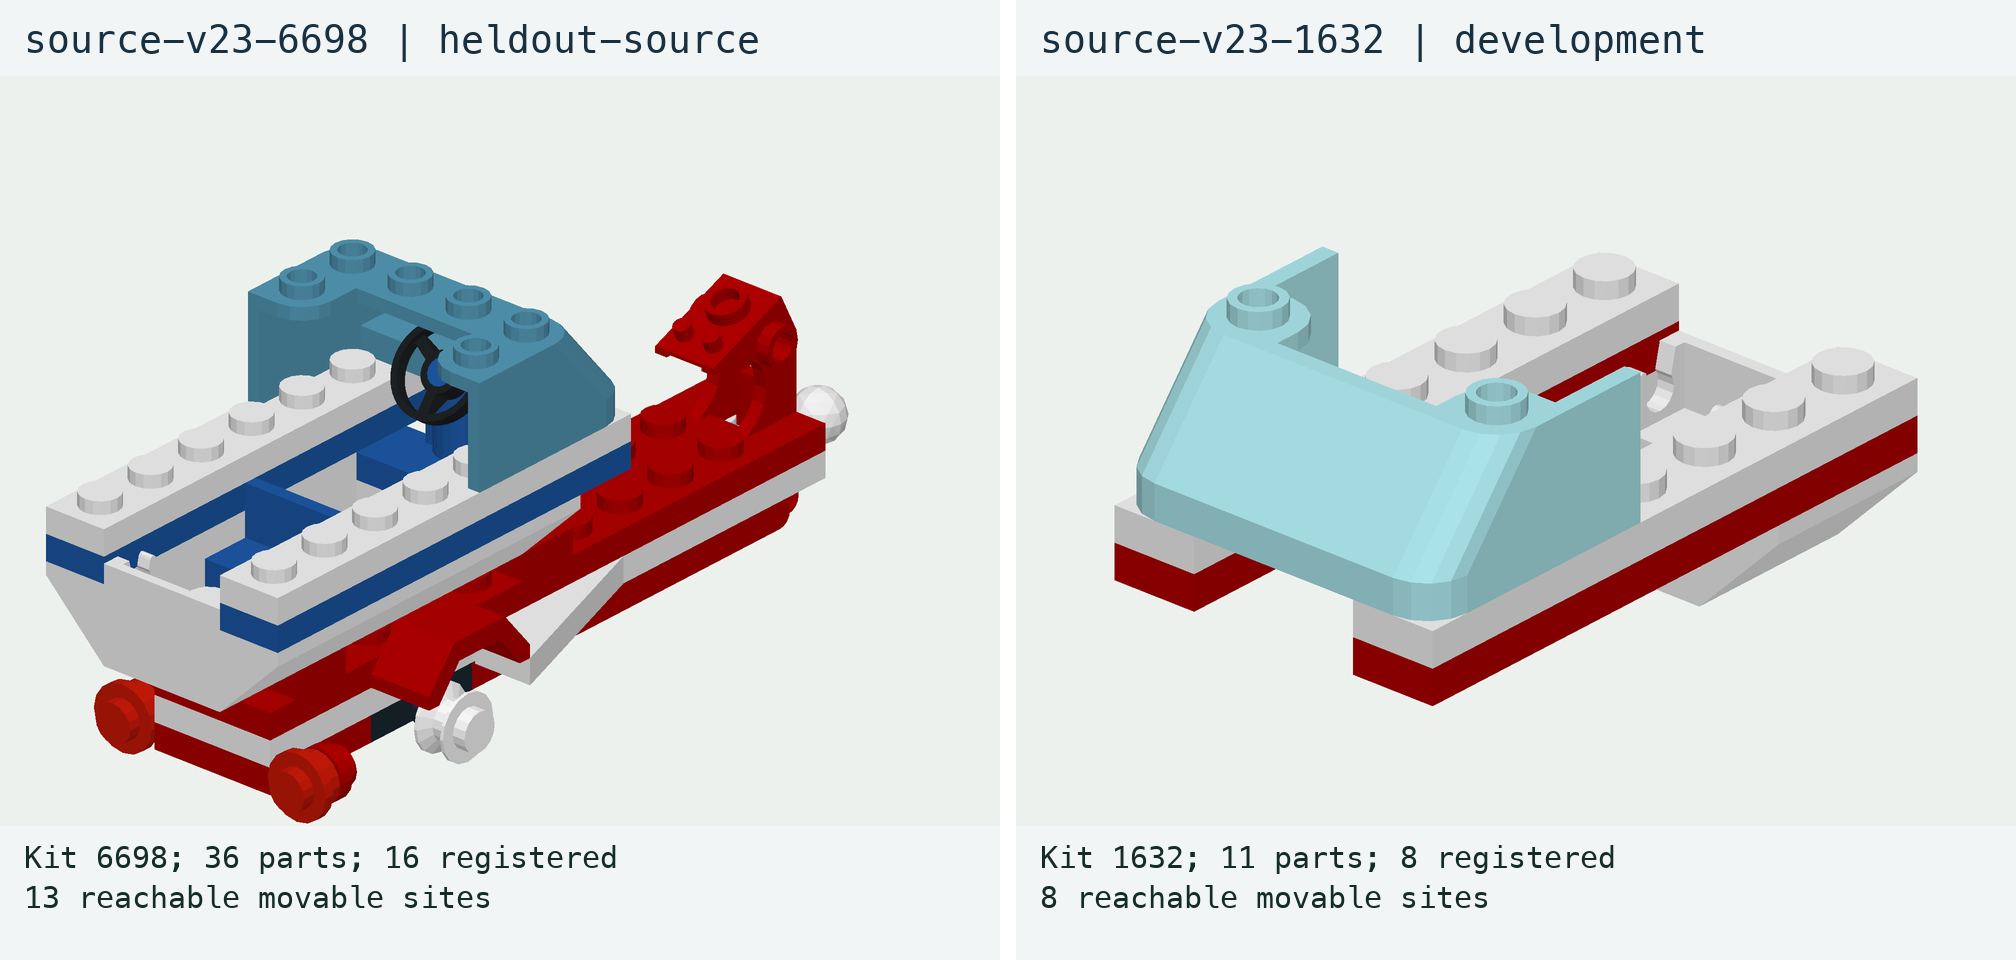
\includegraphics[width=.96\textwidth,height=.85\textheight,keepaspectratio]{figures/source-gallery-25.png}
\end{center}


\clearpage
\section{Source-bound main-paper cases}
\GeometryCaseCaption

\medskip
\RepairCaseCaption

\medskip
The caption file is generated from the same in-memory case records as
the images, and its hash is stored in \texttt{figures/provenance.json}.
Each geometry member records its exact question and task IDs, source
group, profile, start, goal, capacity, jobs, private and public proposed
actions, exact label, and full retained inventory. Original source
instance IDs, matrices, manifest and mesh hashes, and removed-instance
sets bind the illustration to the source geometry. Repair provenance
adds pre-error, delayed, and restored states, executed history, shortest
repair actions, and inverse-last excess. These are evaluator annotations;
they are not model inputs or population results.

\section{Structural control distributions}
\begin{center}
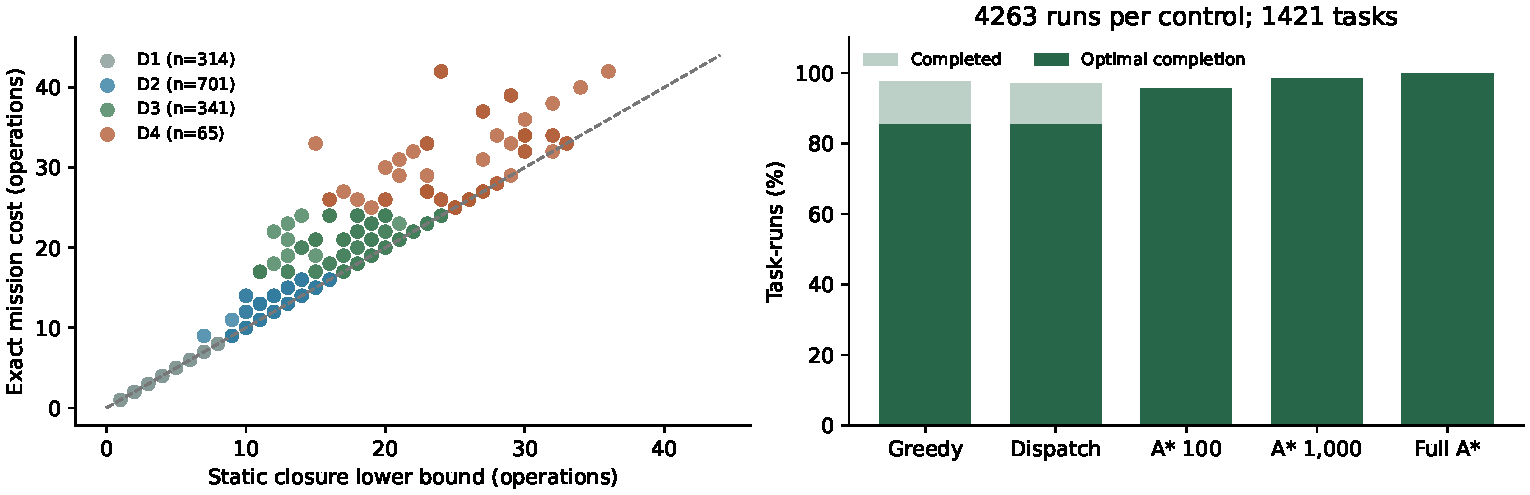
\includegraphics[width=.92\textwidth]{figures/mechanism-evidence.pdf}
\end{center}
Exact costs and static lower bounds are shown with overlapping points.
Completed and optimal task-runs have different denominators from unique
sources. Length bins do not imply monotonic search difficulty. The plot
combines sampling cohorts; the release retains separate split and source
aggregates, and no timing is a calibrated cross-platform comparison.

\clearpage
\section{A certified optimal resource replay}
\begin{center}
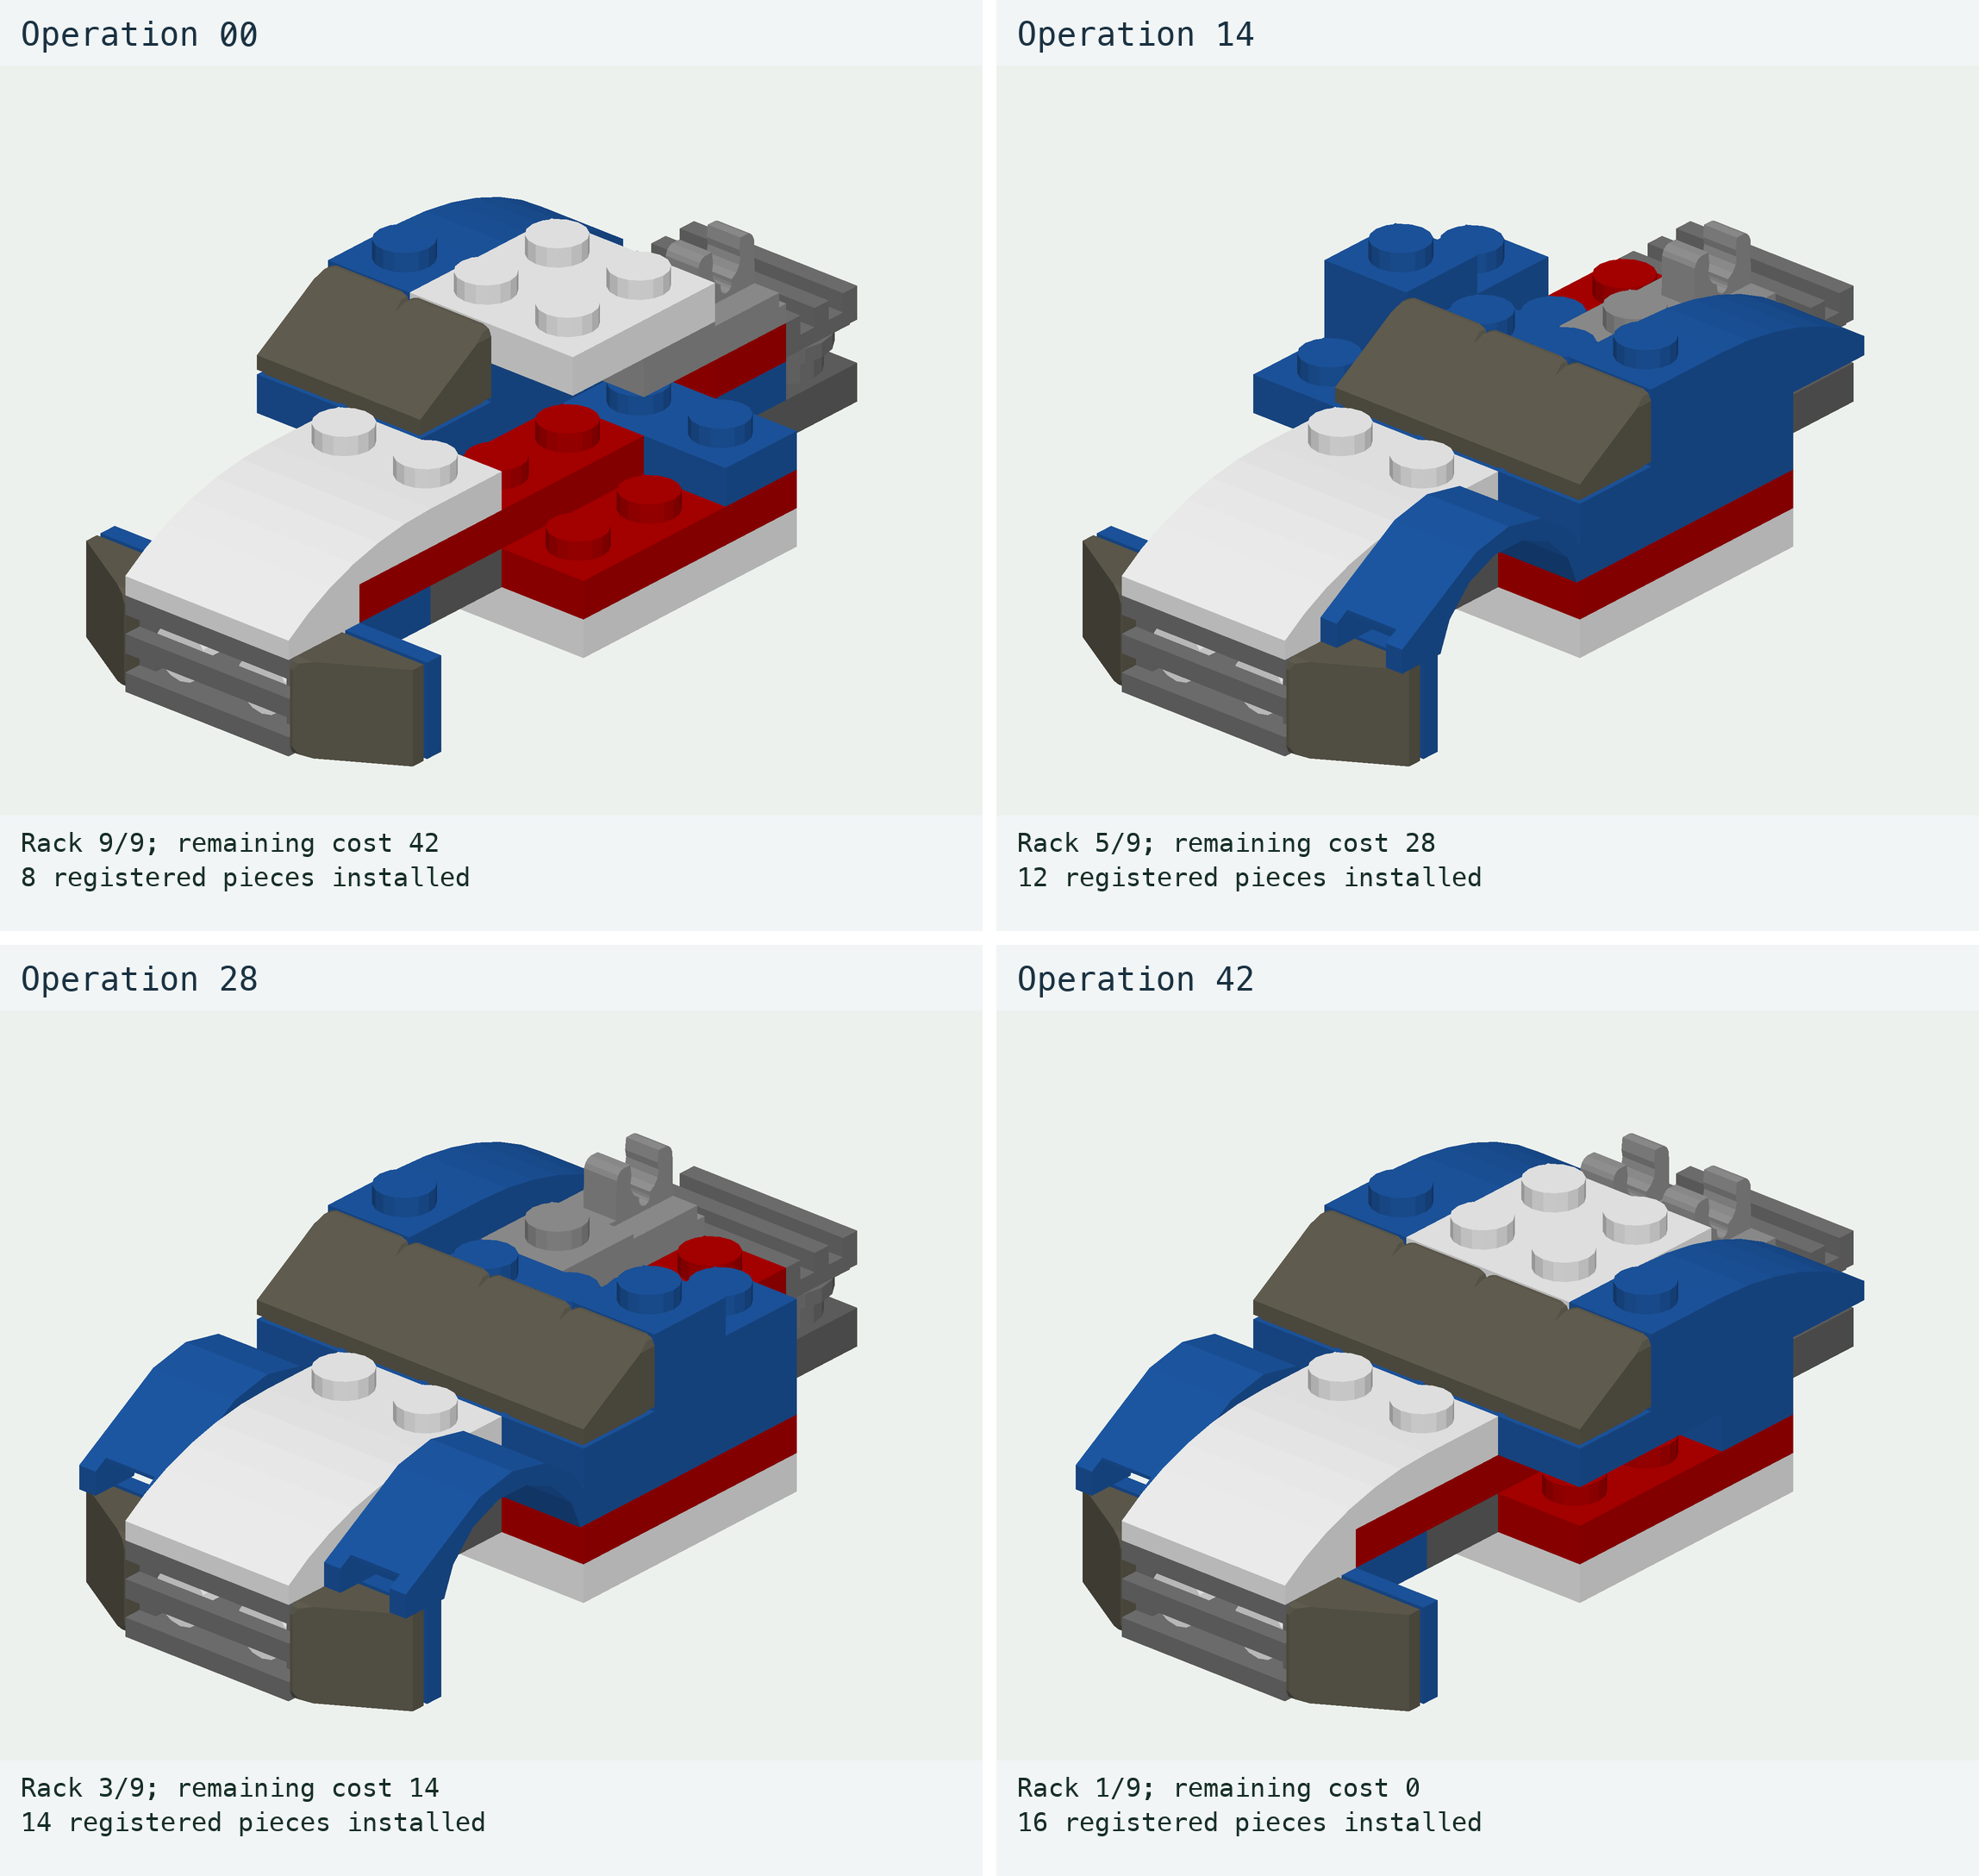
\includegraphics[width=.94\textwidth,height=.76\textheight,keepaspectratio]{figures/resource-replay.png}
\end{center}
\ResourceCaseCaption
All displayed states preserve source poses and certified connectivity.
The figure provenance contains the task ID, seed, occupancy, ledger,
step indices, and exact remaining cost. Rack holders and off-assembly
work are explicit abstractions of the task.

\clearpage
\section{Complete episode census}
``Jobs'' is the declared inspection count, ``Done'' its initially
completed subset, and A* expansions use seed 0 with the closure bound.
D1--D4 are length bins. Internal IDs are evaluator documentation;
participant IDs are consistently permuted by seed. Exact starts, goals,
jobs, witnesses, and oracle paths are available in the task bank.
\small
\begin{longtable}{p{.43\textwidth}lrrrrrr}\toprule
Episode & Tier & Rack & Jobs & Done & $C^*$ & $h$ & A* exp.\\\midrule
\endfirsthead
\toprule
Episode & Tier & Rack & Jobs & Done & $C^*$ & $h$ & A* exp.\\\midrule\endhead
\midrule\endfoot
\bottomrule\endlastfoot
roadster-body-01 & D3 & 17 & 0 & 0 & 17 & 17 & 17\\
roadster-body-02 & D4 & 17 & 0 & 0 & 32 & 32 & 32\\
roadster-body-03 & D4 & 9 & 0 & 0 & 27 & 23 & 33\\
roadster-body-04 & D4 & 9 & 0 & 0 & 27 & 23 & 38\\
roadster-body-05 & D4 & 9 & 0 & 0 & 42 & 24 & 2,555\\
roadster-body-06 & D4 & 9 & 0 & 0 & 42 & 24 & 2,555\\
roadster-body-07 & D4 & 9 & 2 & 0 & 37 & 27 & 2,185\\
roadster-body-08 & D4 & 9 & 2 & 0 & 37 & 27 & 2,139\\
roadster-body-09 & D3 & 9 & 2 & 1 & 20 & 20 & 21\\
roadster-body-10 & D3 & 9 & 2 & 1 & 18 & 18 & 18\\
roadster-body-11 & D3 & 9 & 1 & 0 & 18 & 18 & 18\\
roadster-body-12 & D3 & 9 & 1 & 0 & 18 & 18 & 18\\
roadster-body-13 & D4 & 9 & 4 & 0 & 39 & 29 & 2,131\\
roadster-body-14 & D4 & 9 & 4 & 0 & 39 & 29 & 2,129\\
kart-deck-01 & D3 & 18 & 0 & 0 & 18 & 18 & 18\\
kart-deck-02 & D4 & 18 & 0 & 0 & 25 & 25 & 25\\
kart-deck-03 & D3 & 5 & 0 & 0 & 17 & 11 & 32\\
kart-deck-04 & D3 & 5 & 0 & 0 & 17 & 11 & 32\\
kart-deck-05 & D4 & 5 & 0 & 0 & 26 & 18 & 119\\
kart-deck-06 & D3 & 5 & 0 & 0 & 24 & 16 & 90\\
kart-deck-07 & D4 & 5 & 2 & 0 & 31 & 21 & 121\\
kart-deck-08 & D4 & 5 & 2 & 0 & 29 & 21 & 218\\
kart-deck-09 & D3 & 5 & 2 & 1 & 21 & 15 & 68\\
kart-deck-10 & D3 & 5 & 2 & 1 & 23 & 19 & 42\\
kart-deck-11 & D3 & 5 & 1 & 0 & 23 & 19 & 42\\
kart-deck-12 & D3 & 5 & 1 & 0 & 21 & 15 & 68\\
kart-deck-13 & D4 & 5 & 4 & 0 & 33 & 23 & 403\\
kart-deck-14 & D4 & 5 & 4 & 0 & 33 & 23 & 392\\
airframe-01 & D3 & 21 & 0 & 0 & 21 & 21 & 21\\
airframe-02 & D4 & 21 & 0 & 0 & 33 & 33 & 33\\
airframe-03 & D2 & 8 & 0 & 0 & 16 & 14 & 16\\
airframe-04 & D2 & 8 & 0 & 0 & 16 & 14 & 16\\
airframe-05 & D3 & 8 & 0 & 0 & 17 & 13 & 30\\
airframe-06 & D3 & 8 & 0 & 0 & 17 & 13 & 30\\
airframe-07 & D3 & 8 & 2 & 0 & 22 & 20 & 22\\
airframe-08 & D3 & 8 & 2 & 0 & 22 & 20 & 22\\
airframe-09 & D2 & 8 & 2 & 1 & 9 & 9 & 9\\
airframe-10 & D2 & 8 & 2 & 1 & 9 & 9 & 9\\
airframe-11 & D2 & 8 & 1 & 0 & 9 & 9 & 9\\
airframe-12 & D2 & 8 & 1 & 0 & 9 & 9 & 9\\
airframe-13 & D4 & 8 & 4 & 0 & 26 & 24 & 26\\
airframe-14 & D4 & 8 & 4 & 0 & 26 & 24 & 26\\
truck-cab-01 & D3 & 18 & 0 & 0 & 18 & 18 & 18\\
truck-cab-02 & D4 & 18 & 0 & 0 & 27 & 27 & 27\\
truck-cab-03 & D4 & 12 & 2 & 0 & 40 & 34 & 1,522\\
truck-cab-04 & D4 & 12 & 2 & 0 & 36 & 30 & 809\\
truck-cab-05 & D3 & 12 & 2 & 1 & 21 & 19 & 22\\
truck-cab-06 & D3 & 12 & 2 & 1 & 21 & 19 & 22\\
truck-cab-07 & D3 & 12 & 1 & 0 & 21 & 19 & 22\\
truck-cab-08 & D3 & 12 & 1 & 0 & 21 & 19 & 22\\
truck-cab-09 & D4 & 12 & 4 & 0 & 42 & 36 & 1,546\\
truck-cab-10 & D4 & 12 & 4 & 0 & 38 & 32 & 831\\
house-roof-01 & D3 & 18 & 0 & 0 & 18 & 18 & 18\\
house-roof-02 & D3 & 18 & 0 & 0 & 22 & 22 & 22\\
house-roof-03 & D3 & 5 & 0 & 0 & 21 & 17 & 37\\
house-roof-04 & D3 & 5 & 0 & 0 & 21 & 17 & 37\\
house-roof-05 & D3 & 5 & 0 & 0 & 22 & 18 & 45\\
house-roof-06 & D3 & 5 & 0 & 0 & 22 & 18 & 45\\
house-roof-07 & D4 & 5 & 2 & 0 & 27 & 23 & 54\\
house-roof-08 & D4 & 5 & 2 & 0 & 27 & 23 & 50\\
house-roof-09 & D3 & 5 & 2 & 1 & 17 & 17 & 19\\
house-roof-10 & D3 & 5 & 2 & 1 & 17 & 17 & 23\\
house-roof-11 & D3 & 5 & 1 & 0 & 17 & 17 & 23\\
house-roof-12 & D3 & 5 & 1 & 0 & 17 & 17 & 19\\
house-roof-13 & D4 & 5 & 4 & 0 & 33 & 29 & 76\\
house-roof-14 & D4 & 5 & 4 & 0 & 31 & 27 & 68\\
sports-body-01 & D2 & 22 & 0 & 0 & 10 & 10 & 10\\
sports-body-02 & D2 & 22 & 0 & 0 & 11 & 11 & 11\\
sports-body-03 & D3 & 8 & 2 & 0 & 17 & 17 & 17\\
source-10001-01 & D1 & 2 & 0 & 0 & 2 & 2 & 2\\
source-10001-02 & D1 & 2 & 0 & 0 & 1 & 1 & 1\\
source-10001-03 & D1 & 2 & 2 & 0 & 5 & 5 & 5\\
source-10001-04 & D1 & 2 & 2 & 0 & 6 & 6 & 6\\
source-10001-05 & D1 & 2 & 0 & 0 & 2 & 2 & 2\\
source-10001-06 & D1 & 2 & 0 & 0 & 1 & 1 & 1\\
source-10001-07 & D1 & 2 & 2 & 0 & 4 & 4 & 4\\
source-10001-08 & D1 & 2 & 2 & 0 & 4 & 4 & 4\\
source-10159-01 & D2 & 10 & 0 & 0 & 11 & 11 & 11\\
source-10159-02 & D2 & 10 & 0 & 0 & 9 & 9 & 9\\
source-10159-03 & D2 & 10 & 2 & 0 & 12 & 12 & 12\\
source-10159-04 & D2 & 10 & 2 & 0 & 11 & 11 & 11\\
source-10159-05 & D3 & 10 & 4 & 0 & 21 & 21 & 21\\
source-10159-06 & D2 & 10 & 4 & 0 & 14 & 14 & 14\\
source-10159-07 & D2 & 10 & 0 & 0 & 10 & 10 & 10\\
source-10159-08 & D2 & 10 & 0 & 0 & 14 & 12 & 45\\
source-10159-09 & D2 & 10 & 2 & 0 & 14 & 14 & 14\\
source-10159-10 & D2 & 10 & 2 & 0 & 9 & 9 & 9\\
source-10159-11 & D2 & 10 & 4 & 0 & 12 & 12 & 12\\
source-10159-12 & D2 & 10 & 4 & 0 & 16 & 16 & 16\\
source-10220-01 & D1 & 10 & 0 & 0 & 8 & 8 & 8\\
source-10220-02 & D1 & 10 & 0 & 0 & 7 & 7 & 7\\
source-10220-03 & D2 & 10 & 2 & 0 & 14 & 14 & 14\\
source-10220-04 & D2 & 10 & 2 & 0 & 13 & 13 & 13\\
source-10220-05 & D2 & 10 & 4 & 0 & 14 & 14 & 14\\
source-10220-06 & D3 & 10 & 4 & 0 & 19 & 19 & 19\\
source-10220-07 & D1 & 10 & 0 & 0 & 7 & 7 & 7\\
source-10220-08 & D2 & 10 & 0 & 0 & 11 & 11 & 11\\
source-10220-09 & D2 & 10 & 2 & 0 & 12 & 12 & 12\\
source-10220-10 & D2 & 10 & 2 & 0 & 10 & 10 & 10\\
source-10220-11 & D2 & 10 & 4 & 0 & 14 & 14 & 14\\
source-10220-12 & D2 & 10 & 4 & 0 & 14 & 14 & 14\\
source-10014-01 & D2 & 10 & 0 & 0 & 10 & 10 & 10\\
source-10014-02 & D3 & 10 & 0 & 0 & 21 & 21 & 22\\
source-10014-03 & D2 & 10 & 2 & 0 & 10 & 10 & 10\\
source-10014-04 & D3 & 10 & 2 & 0 & 20 & 20 & 20\\
source-10014-05 & D4 & 10 & 4 & 0 & 26 & 26 & 29\\
source-10014-06 & D3 & 10 & 4 & 0 & 21 & 21 & 21\\
source-10014-07 & D1 & 10 & 0 & 0 & 8 & 8 & 8\\
source-10014-08 & D2 & 10 & 0 & 0 & 15 & 15 & 15\\
source-10014-09 & D2 & 10 & 2 & 0 & 14 & 12 & 58\\
source-10014-10 & D2 & 10 & 2 & 0 & 14 & 14 & 15\\
source-10014-11 & D3 & 10 & 4 & 0 & 21 & 17 & 4,372\\
source-10014-12 & D2 & 10 & 4 & 0 & 15 & 13 & 52\\
source-10128-01 & D1 & 10 & 0 & 0 & 5 & 5 & 5\\
source-10128-02 & D2 & 10 & 0 & 0 & 14 & 14 & 14\\
source-10128-03 & D2 & 10 & 2 & 0 & 15 & 15 & 15\\
source-10128-04 & D3 & 10 & 2 & 0 & 18 & 18 & 18\\
source-10128-05 & D3 & 10 & 4 & 0 & 24 & 24 & 24\\
source-10128-06 & D3 & 10 & 4 & 0 & 18 & 18 & 18\\
source-10128-07 & D2 & 10 & 0 & 0 & 10 & 10 & 10\\
source-10128-08 & D1 & 10 & 0 & 0 & 8 & 8 & 8\\
source-10128-09 & D2 & 10 & 2 & 0 & 11 & 11 & 11\\
source-10128-10 & D2 & 10 & 2 & 0 & 14 & 14 & 22\\
source-10128-11 & D2 & 10 & 4 & 0 & 15 & 15 & 15\\
source-10128-12 & D3 & 10 & 4 & 0 & 19 & 19 & 19\\
source-omr-31031-01 & D2 & 8 & 0 & 0 & 12 & 12 & 12\\
source-omr-31031-02 & D1 & 8 & 0 & 0 & 6 & 6 & 6\\
source-omr-31031-03 & D2 & 8 & 2 & 0 & 13 & 13 & 13\\
source-omr-31031-04 & D2 & 8 & 2 & 0 & 11 & 11 & 11\\
source-omr-31031-05 & D3 & 8 & 4 & 0 & 17 & 17 & 17\\
source-omr-31031-06 & D3 & 8 & 4 & 0 & 20 & 20 & 20\\
source-omr-31031-07 & D2 & 8 & 0 & 0 & 13 & 11 & 26\\
source-omr-31031-08 & D2 & 8 & 0 & 0 & 15 & 15 & 23\\
source-omr-31031-09 & D1 & 8 & 2 & 0 & 8 & 8 & 8\\
source-omr-31031-10 & D2 & 8 & 2 & 0 & 10 & 10 & 10\\
source-omr-31031-11 & D2 & 8 & 4 & 0 & 14 & 14 & 14\\
source-omr-31031-12 & D2 & 8 & 4 & 0 & 15 & 15 & 15\\
roadster-body-context-0-01 & D4 & 9 & 1 & 0 & 34 & 32 & 954\\
roadster-body-context-1-01 & D4 & 9 & 1 & 0 & 34 & 32 & 953\\
roadster-body-context-0-02 & D4 & 9 & 1 & 0 & 34 & 30 & 1,018\\
roadster-body-context-1-02 & D4 & 9 & 1 & 0 & 34 & 30 & 1,017\\
roadster-body-context-0-03 & D4 & 9 & 1 & 0 & 34 & 30 & 847\\
roadster-body-context-1-03 & D4 & 9 & 1 & 0 & 34 & 30 & 846\\
roadster-body-context-0-04 & D4 & 9 & 1 & 0 & 32 & 30 & 414\\
roadster-body-context-1-04 & D4 & 9 & 1 & 0 & 32 & 30 & 413\\
source-10036-01 & D2 & 10 & 0 & 0 & 16 & 16 & 16\\
source-10036-02 & D1 & 10 & 0 & 0 & 8 & 8 & 8\\
source-10036-03 & D2 & 10 & 0 & 0 & 12 & 12 & 12\\
source-10036-04 & D4 & 10 & 0 & 0 & 29 & 23 & 406\\
source-10036-05 & D2 & 10 & 2 & 0 & 16 & 16 & 16\\
source-10036-06 & D3 & 10 & 2 & 0 & 17 & 17 & 17\\
source-10036-07 & D3 & 10 & 2 & 0 & 17 & 17 & 17\\
source-10036-08 & D2 & 10 & 2 & 0 & 15 & 15 & 15\\
source-10036-09 & D4 & 10 & 4 & 0 & 27 & 27 & 27\\
source-10036-10 & D3 & 10 & 4 & 0 & 24 & 24 & 24\\
source-10036-11 & D4 & 10 & 4 & 0 & 26 & 26 & 26\\
source-10036-12 & D4 & 10 & 4 & 0 & 34 & 28 & 7,595\\
source-10036-13 & D2 & 10 & 0 & 0 & 11 & 11 & 11\\
source-10036-14 & D2 & 10 & 0 & 0 & 10 & 10 & 10\\
source-10036-15 & D2 & 10 & 0 & 0 & 15 & 15 & 27\\
source-10036-16 & D2 & 10 & 0 & 0 & 12 & 12 & 12\\
source-10036-17 & D2 & 10 & 2 & 0 & 16 & 16 & 22\\
source-10036-18 & D4 & 10 & 2 & 0 & 26 & 16 & 3,168\\
source-10036-19 & D3 & 10 & 2 & 0 & 24 & 14 & 2,226\\
source-10036-20 & D2 & 10 & 2 & 0 & 14 & 14 & 21\\
source-10036-21 & D4 & 10 & 4 & 0 & 30 & 20 & 12,578\\
source-10036-22 & D3 & 10 & 4 & 0 & 24 & 18 & 1,714\\
source-10036-23 & D3 & 10 & 4 & 0 & 19 & 19 & 27\\
source-10036-24 & D3 & 10 & 4 & 0 & 20 & 20 & 56\\
source-10036-25 & D2 & 10 & 0 & 0 & 10 & 10 & 10\\
source-10036-26 & D1 & 10 & 0 & 0 & 6 & 6 & 6\\
source-10036-27 & D2 & 10 & 0 & 0 & 16 & 16 & 16\\
source-10036-28 & D2 & 10 & 0 & 0 & 9 & 9 & 9\\
source-10036-29 & D2 & 10 & 2 & 0 & 13 & 13 & 13\\
source-10036-30 & D2 & 10 & 2 & 0 & 13 & 13 & 13\\
source-10036-31 & D2 & 10 & 2 & 0 & 12 & 12 & 12\\
source-10036-32 & D2 & 10 & 2 & 0 & 13 & 11 & 14\\
source-10036-33 & D3 & 10 & 4 & 0 & 20 & 20 & 20\\
source-10036-34 & D3 & 10 & 4 & 0 & 22 & 22 & 22\\
source-10036-35 & D3 & 10 & 4 & 0 & 22 & 18 & 134\\
source-10036-36 & D3 & 10 & 4 & 0 & 22 & 22 & 22\\
source-10036-37 & D2 & 10 & 0 & 0 & 14 & 12 & 60\\
source-10036-38 & D4 & 10 & 0 & 0 & 27 & 17 & 786\\
source-10036-39 & D3 & 10 & 0 & 0 & 20 & 14 & 264\\
source-10036-40 & D1 & 10 & 0 & 0 & 5 & 5 & 7\\
source-10036-41 & D4 & 10 & 2 & 0 & 33 & 15 & 4,640\\
source-10036-42 & D3 & 10 & 2 & 0 & 17 & 11 & 282\\
source-10036-43 & D2 & 10 & 2 & 0 & 14 & 12 & 101\\
source-10036-44 & D3 & 10 & 2 & 0 & 19 & 17 & 236\\
source-10036-45 & D3 & 10 & 4 & 0 & 19 & 15 & 726\\
source-10036-46 & D2 & 10 & 4 & 0 & 15 & 13 & 151\\
source-10036-47 & D4 & 10 & 4 & 0 & 32 & 22 & 11,933\\
source-10036-48 & D2 & 10 & 4 & 0 & 14 & 10 & 311\\
source-10213-01 & D1 & 2 & 0 & 0 & 2 & 2 & 2\\
source-10213-02 & D1 & 2 & 0 & 0 & 1 & 1 & 1\\
source-10213-03 & D1 & 2 & 0 & 0 & 1 & 1 & 1\\
source-10213-04 & D1 & 2 & 2 & 0 & 6 & 6 & 6\\
source-10213-05 & D1 & 2 & 2 & 0 & 4 & 4 & 4\\
source-10213-06 & D1 & 2 & 2 & 0 & 5 & 5 & 5\\
source-10213-07 & D1 & 2 & 2 & 0 & 5 & 5 & 5\\
source-10213-08 & D1 & 2 & 0 & 0 & 2 & 2 & 2\\
source-10213-09 & D1 & 2 & 0 & 0 & 1 & 1 & 1\\
source-10213-10 & D1 & 2 & 0 & 0 & 1 & 1 & 1\\
source-10213-11 & D1 & 2 & 2 & 0 & 4 & 4 & 4\\
source-10213-12 & D1 & 2 & 2 & 0 & 2 & 2 & 2\\
source-10213-13 & D1 & 2 & 2 & 0 & 3 & 3 & 3\\
source-10213-14 & D1 & 2 & 2 & 0 & 3 & 3 & 3\\
source-10213-15 & D1 & 2 & 0 & 0 & 1 & 1 & 1\\
source-10213-16 & D1 & 2 & 0 & 0 & 2 & 2 & 2\\
source-10213-17 & D1 & 2 & 0 & 0 & 1 & 1 & 1\\
source-10213-18 & D1 & 2 & 2 & 0 & 4 & 4 & 4\\
source-10213-19 & D1 & 2 & 2 & 0 & 5 & 5 & 5\\
source-10213-20 & D1 & 2 & 2 & 0 & 4 & 4 & 4\\
source-10213-21 & D1 & 2 & 2 & 0 & 3 & 3 & 3\\
source-10213-22 & D1 & 2 & 0 & 0 & 1 & 1 & 1\\
source-10213-23 & D1 & 2 & 0 & 0 & 1 & 1 & 1\\
source-10213-24 & D1 & 2 & 0 & 0 & 2 & 2 & 2\\
source-10213-25 & D1 & 2 & 2 & 0 & 3 & 3 & 3\\
source-10213-26 & D1 & 2 & 2 & 0 & 4 & 4 & 4\\
source-10213-27 & D1 & 2 & 2 & 0 & 5 & 5 & 5\\
source-10213-28 & D1 & 2 & 2 & 0 & 4 & 4 & 4\\
source-omr-10242-01 & D1 & 10 & 0 & 0 & 8 & 8 & 8\\
source-omr-10242-02 & D2 & 10 & 0 & 0 & 14 & 14 & 14\\
source-omr-10242-03 & D1 & 10 & 0 & 0 & 7 & 7 & 7\\
source-omr-10242-04 & D2 & 10 & 0 & 0 & 11 & 11 & 11\\
source-omr-10242-05 & D2 & 10 & 2 & 0 & 13 & 13 & 13\\
source-omr-10242-06 & D2 & 10 & 2 & 0 & 16 & 16 & 16\\
source-omr-10242-07 & D2 & 10 & 2 & 0 & 11 & 11 & 11\\
source-omr-10242-08 & D2 & 10 & 2 & 0 & 15 & 15 & 15\\
source-omr-10242-09 & D3 & 10 & 4 & 0 & 17 & 17 & 17\\
source-omr-10242-10 & D2 & 10 & 4 & 0 & 16 & 16 & 16\\
source-omr-10242-11 & D2 & 10 & 4 & 0 & 14 & 14 & 14\\
source-omr-10242-12 & D3 & 10 & 4 & 0 & 17 & 17 & 17\\
source-omr-10242-13 & D2 & 10 & 0 & 0 & 9 & 9 & 9\\
source-omr-10242-14 & D1 & 10 & 0 & 0 & 7 & 7 & 7\\
source-omr-10242-15 & D2 & 10 & 0 & 0 & 9 & 9 & 9\\
source-omr-10242-16 & D1 & 10 & 0 & 0 & 8 & 8 & 8\\
source-omr-10242-17 & D2 & 10 & 2 & 0 & 13 & 13 & 13\\
source-omr-10242-18 & D2 & 10 & 2 & 0 & 16 & 16 & 16\\
source-omr-10242-19 & D2 & 10 & 2 & 0 & 12 & 12 & 12\\
source-omr-10242-20 & D2 & 10 & 2 & 0 & 12 & 12 & 12\\
source-omr-10242-21 & D2 & 10 & 4 & 0 & 14 & 14 & 14\\
source-omr-10242-22 & D2 & 10 & 4 & 0 & 13 & 13 & 13\\
source-omr-10242-23 & D2 & 10 & 4 & 0 & 13 & 13 & 13\\
source-omr-10242-24 & D2 & 10 & 4 & 0 & 15 & 15 & 15\\
source-omr-10242-25 & D2 & 10 & 0 & 0 & 11 & 11 & 11\\
source-omr-10242-26 & D1 & 10 & 0 & 0 & 7 & 7 & 7\\
source-omr-10242-27 & D1 & 10 & 0 & 0 & 6 & 6 & 6\\
source-omr-10242-28 & D2 & 10 & 0 & 0 & 10 & 10 & 10\\
source-omr-10242-29 & D2 & 10 & 2 & 0 & 9 & 9 & 9\\
source-omr-10242-30 & D3 & 10 & 2 & 0 & 17 & 17 & 17\\
source-omr-10242-31 & D2 & 10 & 2 & 0 & 10 & 10 & 10\\
source-omr-10242-32 & D2 & 10 & 2 & 0 & 12 & 12 & 12\\
source-omr-10242-33 & D2 & 10 & 4 & 0 & 14 & 14 & 14\\
source-omr-10242-34 & D2 & 10 & 4 & 0 & 14 & 14 & 14\\
source-omr-10242-35 & D2 & 10 & 4 & 0 & 15 & 15 & 15\\
source-omr-10242-36 & D2 & 10 & 4 & 0 & 14 & 14 & 14\\
source-omr-10242-37 & D2 & 10 & 0 & 0 & 10 & 10 & 10\\
source-omr-10242-38 & D1 & 10 & 0 & 0 & 8 & 8 & 8\\
source-omr-10242-39 & D1 & 10 & 0 & 0 & 7 & 7 & 7\\
source-omr-10242-40 & D1 & 10 & 0 & 0 & 8 & 8 & 8\\
source-omr-10242-41 & D2 & 10 & 2 & 0 & 10 & 10 & 10\\
source-omr-10242-42 & D2 & 10 & 2 & 0 & 11 & 11 & 11\\
source-omr-10242-43 & D2 & 10 & 2 & 0 & 11 & 11 & 11\\
source-omr-10242-44 & D2 & 10 & 2 & 0 & 12 & 12 & 12\\
source-omr-10242-45 & D2 & 10 & 4 & 0 & 16 & 16 & 16\\
source-omr-10242-46 & D3 & 10 & 4 & 0 & 17 & 17 & 17\\
source-omr-10242-47 & D3 & 10 & 4 & 0 & 17 & 17 & 17\\
source-omr-10242-48 & D3 & 10 & 4 & 0 & 18 & 18 & 18\\
source-omr-10265-01 & D1 & 3 & 0 & 0 & 2 & 2 & 2\\
source-omr-10265-02 & D1 & 3 & 0 & 0 & 1 & 1 & 1\\
source-omr-10265-03 & D1 & 3 & 0 & 0 & 1 & 1 & 1\\
source-omr-10265-04 & D1 & 3 & 0 & 0 & 3 & 3 & 3\\
source-omr-10265-05 & D1 & 3 & 2 & 0 & 5 & 5 & 5\\
source-omr-10265-06 & D1 & 3 & 2 & 0 & 7 & 7 & 7\\
source-omr-10265-07 & D1 & 3 & 2 & 0 & 4 & 4 & 4\\
source-omr-10265-08 & D1 & 3 & 2 & 0 & 5 & 5 & 5\\
source-omr-10265-09 & D2 & 3 & 4 & 0 & 9 & 9 & 9\\
source-omr-10265-10 & D2 & 3 & 4 & 0 & 10 & 10 & 10\\
source-omr-10265-11 & D2 & 3 & 4 & 0 & 12 & 12 & 12\\
source-omr-10265-12 & D2 & 3 & 4 & 0 & 9 & 9 & 9\\
source-omr-10265-13 & D1 & 3 & 0 & 0 & 2 & 2 & 2\\
source-omr-10265-14 & D1 & 3 & 0 & 0 & 2 & 2 & 2\\
source-omr-10265-15 & D1 & 3 & 0 & 0 & 2 & 2 & 2\\
source-omr-10265-16 & D1 & 3 & 0 & 0 & 1 & 1 & 1\\
source-omr-10265-17 & D1 & 3 & 2 & 0 & 4 & 4 & 4\\
source-omr-10265-18 & D1 & 3 & 2 & 0 & 7 & 7 & 7\\
source-omr-10265-19 & D1 & 3 & 2 & 0 & 5 & 5 & 5\\
source-omr-10265-20 & D1 & 3 & 2 & 0 & 5 & 5 & 5\\
source-omr-10265-21 & D2 & 3 & 4 & 0 & 9 & 9 & 9\\
source-omr-10265-22 & D2 & 3 & 4 & 0 & 9 & 9 & 9\\
source-omr-10265-23 & D2 & 3 & 4 & 0 & 9 & 9 & 9\\
source-omr-10265-24 & D2 & 3 & 4 & 0 & 9 & 9 & 9\\
source-omr-10265-25 & D1 & 3 & 0 & 0 & 2 & 2 & 2\\
source-omr-10265-26 & D1 & 3 & 0 & 0 & 3 & 3 & 3\\
source-omr-10265-27 & D1 & 3 & 0 & 0 & 3 & 3 & 3\\
source-omr-10265-28 & D1 & 3 & 0 & 0 & 2 & 2 & 2\\
source-omr-10265-29 & D1 & 3 & 2 & 0 & 3 & 3 & 3\\
source-omr-10265-30 & D1 & 3 & 2 & 0 & 4 & 4 & 4\\
source-omr-10265-31 & D1 & 3 & 2 & 0 & 5 & 5 & 5\\
source-omr-10265-32 & D1 & 3 & 2 & 0 & 5 & 5 & 5\\
source-omr-10265-33 & D1 & 3 & 4 & 0 & 7 & 7 & 7\\
source-omr-10265-34 & D1 & 3 & 4 & 0 & 7 & 7 & 7\\
source-omr-10265-35 & D1 & 3 & 4 & 0 & 7 & 7 & 7\\
source-omr-10265-36 & D1 & 3 & 4 & 0 & 8 & 8 & 8\\
source-omr-10265-37 & D1 & 3 & 0 & 0 & 2 & 2 & 2\\
source-omr-10265-38 & D1 & 3 & 0 & 0 & 3 & 3 & 3\\
source-omr-10265-39 & D1 & 3 & 0 & 0 & 1 & 1 & 1\\
source-omr-10265-40 & D1 & 3 & 0 & 0 & 1 & 1 & 1\\
source-omr-10265-41 & D1 & 3 & 2 & 0 & 8 & 8 & 8\\
source-omr-10265-42 & D1 & 3 & 2 & 0 & 6 & 6 & 6\\
source-omr-10265-43 & D1 & 3 & 2 & 0 & 7 & 7 & 7\\
source-omr-10265-44 & D1 & 3 & 2 & 0 & 6 & 6 & 6\\
source-omr-10265-45 & D2 & 3 & 4 & 0 & 9 & 9 & 9\\
source-omr-10265-46 & D2 & 3 & 4 & 0 & 9 & 9 & 9\\
source-omr-10265-47 & D2 & 3 & 4 & 0 & 9 & 9 & 9\\
source-omr-10265-48 & D1 & 3 & 4 & 0 & 8 & 8 & 8\\
source-omr-10269-01 & D2 & 10 & 0 & 0 & 11 & 11 & 11\\
source-omr-10269-02 & D2 & 10 & 0 & 0 & 13 & 13 & 13\\
source-omr-10269-03 & D2 & 10 & 0 & 0 & 12 & 12 & 12\\
source-omr-10269-04 & D2 & 10 & 0 & 0 & 9 & 9 & 9\\
source-omr-10269-05 & D3 & 10 & 2 & 0 & 17 & 17 & 17\\
source-omr-10269-06 & D3 & 10 & 2 & 0 & 18 & 18 & 18\\
source-omr-10269-07 & D2 & 10 & 2 & 0 & 16 & 16 & 16\\
source-omr-10269-08 & D2 & 10 & 2 & 0 & 15 & 15 & 15\\
source-omr-10269-09 & D3 & 10 & 4 & 0 & 22 & 22 & 22\\
source-omr-10269-10 & D3 & 10 & 4 & 0 & 21 & 21 & 21\\
source-omr-10269-11 & D3 & 10 & 4 & 0 & 19 & 19 & 19\\
source-omr-10269-12 & D3 & 10 & 4 & 0 & 20 & 20 & 20\\
source-omr-10269-13 & D1 & 10 & 0 & 0 & 6 & 6 & 6\\
source-omr-10269-14 & D2 & 10 & 0 & 0 & 11 & 11 & 11\\
source-omr-10269-15 & D2 & 10 & 0 & 0 & 10 & 10 & 10\\
source-omr-10269-16 & D1 & 10 & 0 & 0 & 7 & 7 & 7\\
source-omr-10269-17 & D2 & 10 & 2 & 0 & 14 & 14 & 14\\
source-omr-10269-18 & D2 & 10 & 2 & 0 & 15 & 15 & 15\\
source-omr-10269-19 & D2 & 10 & 2 & 0 & 11 & 11 & 11\\
source-omr-10269-20 & D2 & 10 & 2 & 0 & 12 & 12 & 12\\
source-omr-10269-21 & D3 & 10 & 4 & 0 & 18 & 18 & 18\\
source-omr-10269-22 & D2 & 10 & 4 & 0 & 16 & 16 & 16\\
source-omr-10269-23 & D2 & 10 & 4 & 0 & 13 & 13 & 13\\
source-omr-10269-24 & D2 & 10 & 4 & 0 & 14 & 14 & 14\\
source-omr-10269-25 & D2 & 10 & 0 & 0 & 14 & 14 & 14\\
source-omr-10269-26 & D1 & 10 & 0 & 0 & 7 & 7 & 7\\
source-omr-10269-27 & D2 & 10 & 0 & 0 & 11 & 11 & 11\\
source-omr-10269-28 & D2 & 10 & 0 & 0 & 10 & 10 & 10\\
source-omr-10269-29 & D2 & 10 & 2 & 0 & 12 & 12 & 12\\
source-omr-10269-30 & D2 & 10 & 2 & 0 & 13 & 13 & 13\\
source-omr-10269-31 & D2 & 10 & 2 & 0 & 14 & 14 & 14\\
source-omr-10269-32 & D2 & 10 & 2 & 0 & 12 & 12 & 12\\
source-omr-10269-33 & D2 & 10 & 4 & 0 & 15 & 15 & 15\\
source-omr-10269-34 & D3 & 10 & 4 & 0 & 17 & 17 & 17\\
source-omr-10269-35 & D2 & 10 & 4 & 0 & 14 & 14 & 14\\
source-omr-10269-36 & D2 & 10 & 4 & 0 & 15 & 15 & 15\\
source-omr-10269-37 & D2 & 10 & 0 & 0 & 12 & 12 & 12\\
source-omr-10269-38 & D2 & 10 & 0 & 0 & 13 & 13 & 13\\
source-omr-10269-39 & D2 & 10 & 0 & 0 & 12 & 12 & 12\\
source-omr-10269-40 & D1 & 10 & 0 & 0 & 8 & 8 & 8\\
source-omr-10269-41 & D2 & 10 & 2 & 0 & 15 & 15 & 15\\
source-omr-10269-42 & D2 & 10 & 2 & 0 & 13 & 13 & 13\\
source-omr-10269-43 & D2 & 10 & 2 & 0 & 12 & 12 & 14\\
source-omr-10269-44 & D2 & 10 & 2 & 0 & 16 & 16 & 16\\
source-omr-10269-45 & D2 & 10 & 4 & 0 & 16 & 16 & 16\\
source-omr-10269-46 & D3 & 10 & 4 & 0 & 18 & 18 & 18\\
source-omr-10269-47 & D3 & 10 & 4 & 0 & 17 & 17 & 17\\
source-omr-10269-48 & D2 & 10 & 4 & 0 & 15 & 15 & 15\\
source-10014-context-0-01 & D3 & 10 & 1 & 0 & 18 & 18 & 23\\
source-10014-context-1-01 & D3 & 10 & 1 & 0 & 18 & 18 & 18\\
source-10014-context-0-02 & D3 & 10 & 1 & 0 & 22 & 22 & 31\\
source-10014-context-1-02 & D3 & 10 & 1 & 0 & 22 & 22 & 22\\
source-10036-context-0-01 & D2 & 10 & 0 & 0 & 15 & 15 & 15\\
source-10036-context-1-01 & D2 & 10 & 0 & 0 & 15 & 15 & 15\\
source-10036-context-0-02 & D2 & 10 & 0 & 0 & 16 & 16 & 16\\
source-10036-context-1-02 & D2 & 10 & 0 & 0 & 16 & 16 & 16\\
source-10036-intervention-2-context-0-01 & D3 & 10 & 0 & 0 & 17 & 17 & 17\\
source-10036-intervention-2-context-1-01 & D3 & 10 & 0 & 0 & 17 & 17 & 17\\
source-10036-intervention-2-context-0-02 & D2 & 10 & 0 & 0 & 15 & 15 & 15\\
source-10036-intervention-2-context-1-02 & D2 & 10 & 0 & 0 & 15 & 15 & 15\\
source-v23-10037-01 & D2 & 10 & 0 & 0 & 9 & 9 & 9\\
source-v23-10037-02 & D2 & 10 & 0 & 0 & 9 & 9 & 9\\
source-v23-10037-03 & D2 & 10 & 2 & 0 & 12 & 12 & 12\\
source-v23-10037-04 & D2 & 10 & 2 & 0 & 12 & 12 & 12\\
source-v23-10037-05 & D2 & 10 & 4 & 0 & 12 & 12 & 12\\
source-v23-10037-06 & D3 & 10 & 4 & 0 & 18 & 18 & 18\\
source-v23-10037-07 & D1 & 10 & 0 & 0 & 6 & 6 & 6\\
source-v23-10037-08 & D2 & 10 & 0 & 0 & 12 & 12 & 12\\
source-v23-10037-09 & D2 & 10 & 2 & 0 & 13 & 13 & 13\\
source-v23-10037-10 & D2 & 10 & 2 & 0 & 11 & 11 & 11\\
source-v23-10037-11 & D2 & 10 & 4 & 0 & 10 & 10 & 10\\
source-v23-10037-12 & D2 & 10 & 4 & 0 & 13 & 13 & 13\\
source-v23-10184-01 & D1 & 10 & 0 & 0 & 7 & 7 & 7\\
source-v23-10184-02 & D1 & 10 & 0 & 0 & 7 & 7 & 7\\
source-v23-10184-03 & D2 & 10 & 2 & 0 & 11 & 11 & 11\\
source-v23-10184-04 & D2 & 10 & 2 & 0 & 13 & 13 & 13\\
source-v23-10184-05 & D2 & 10 & 4 & 0 & 12 & 12 & 12\\
source-v23-10184-06 & D3 & 10 & 4 & 0 & 17 & 17 & 17\\
source-v23-10184-07 & D1 & 10 & 0 & 0 & 5 & 5 & 5\\
source-v23-10184-08 & D1 & 10 & 0 & 0 & 7 & 7 & 7\\
source-v23-10184-09 & D2 & 10 & 2 & 0 & 12 & 12 & 12\\
source-v23-10184-10 & D1 & 10 & 2 & 0 & 7 & 7 & 7\\
source-v23-10184-11 & D2 & 10 & 4 & 0 & 12 & 12 & 12\\
source-v23-10184-12 & D2 & 10 & 4 & 0 & 9 & 9 & 9\\
source-v23-10267-01 & D1 & 10 & 0 & 0 & 5 & 5 & 5\\
source-v23-10267-02 & D2 & 10 & 0 & 0 & 9 & 9 & 9\\
source-v23-10267-03 & D2 & 10 & 2 & 0 & 12 & 12 & 12\\
source-v23-10267-04 & D2 & 10 & 2 & 0 & 15 & 15 & 15\\
source-v23-10267-05 & D3 & 10 & 4 & 0 & 20 & 20 & 20\\
source-v23-10267-06 & D3 & 10 & 4 & 0 & 19 & 19 & 19\\
source-v23-10267-07 & D1 & 10 & 0 & 0 & 8 & 8 & 8\\
source-v23-10267-08 & D1 & 10 & 0 & 0 & 8 & 8 & 8\\
source-v23-10267-09 & D2 & 10 & 2 & 0 & 10 & 10 & 10\\
source-v23-10267-10 & D2 & 10 & 2 & 0 & 13 & 13 & 13\\
source-v23-10267-11 & D2 & 10 & 4 & 0 & 13 & 13 & 13\\
source-v23-10267-12 & D2 & 10 & 4 & 0 & 14 & 14 & 14\\
source-v23-1472-01 & D2 & 10 & 0 & 0 & 10 & 10 & 10\\
source-v23-1472-02 & D1 & 10 & 0 & 0 & 7 & 7 & 7\\
source-v23-1472-03 & D2 & 10 & 2 & 0 & 15 & 15 & 15\\
source-v23-1472-04 & D2 & 10 & 2 & 0 & 13 & 13 & 13\\
source-v23-1472-05 & D3 & 10 & 4 & 0 & 19 & 19 & 19\\
source-v23-1472-06 & D3 & 10 & 4 & 0 & 20 & 20 & 20\\
source-v23-1472-07 & D1 & 10 & 0 & 0 & 5 & 5 & 5\\
source-v23-1472-08 & D1 & 10 & 0 & 0 & 8 & 8 & 8\\
source-v23-1472-09 & D2 & 10 & 2 & 0 & 11 & 11 & 11\\
source-v23-1472-10 & D2 & 10 & 2 & 0 & 12 & 12 & 12\\
source-v23-1472-11 & D2 & 10 & 4 & 0 & 12 & 12 & 12\\
source-v23-1472-12 & D2 & 10 & 4 & 0 & 13 & 13 & 13\\
source-v23-1484-01 & D2 & 10 & 0 & 0 & 12 & 12 & 12\\
source-v23-1484-02 & D3 & 10 & 0 & 0 & 17 & 17 & 17\\
source-v23-1484-03 & D2 & 10 & 2 & 0 & 16 & 16 & 16\\
source-v23-1484-04 & D2 & 10 & 2 & 0 & 16 & 16 & 16\\
source-v23-1484-05 & D3 & 10 & 4 & 0 & 19 & 19 & 19\\
source-v23-1484-06 & D2 & 10 & 4 & 0 & 15 & 15 & 15\\
source-v23-1484-07 & D2 & 10 & 0 & 0 & 10 & 10 & 10\\
source-v23-1484-08 & D2 & 10 & 0 & 0 & 9 & 9 & 9\\
source-v23-1484-09 & D3 & 10 & 2 & 0 & 17 & 17 & 17\\
source-v23-1484-10 & D2 & 10 & 2 & 0 & 14 & 14 & 14\\
source-v23-1484-11 & D2 & 10 & 4 & 0 & 16 & 16 & 16\\
source-v23-1484-12 & D2 & 10 & 4 & 0 & 12 & 12 & 12\\
source-v23-1490-01 & D2 & 10 & 0 & 0 & 10 & 10 & 10\\
source-v23-1490-02 & D2 & 10 & 0 & 0 & 11 & 11 & 11\\
source-v23-1490-03 & D2 & 10 & 2 & 0 & 15 & 15 & 15\\
source-v23-1490-04 & D2 & 10 & 2 & 0 & 15 & 15 & 15\\
source-v23-1490-05 & D3 & 10 & 4 & 0 & 17 & 17 & 17\\
source-v23-1490-06 & D2 & 10 & 4 & 0 & 16 & 16 & 16\\
source-v23-1490-07 & D1 & 10 & 0 & 0 & 5 & 5 & 5\\
source-v23-1490-08 & D2 & 10 & 0 & 0 & 10 & 10 & 10\\
source-v23-1490-09 & D2 & 10 & 2 & 0 & 14 & 14 & 14\\
source-v23-1490-10 & D2 & 10 & 2 & 0 & 12 & 12 & 12\\
source-v23-1490-11 & D2 & 10 & 4 & 0 & 14 & 14 & 14\\
source-v23-1490-12 & D2 & 10 & 4 & 0 & 15 & 15 & 15\\
source-v23-1854-01 & D2 & 10 & 0 & 0 & 9 & 9 & 9\\
source-v23-1854-02 & D2 & 10 & 0 & 0 & 15 & 15 & 15\\
source-v23-1854-03 & D3 & 10 & 2 & 0 & 18 & 18 & 18\\
source-v23-1854-04 & D2 & 10 & 2 & 0 & 11 & 11 & 11\\
source-v23-1854-05 & D3 & 10 & 4 & 0 & 17 & 17 & 17\\
source-v23-1854-06 & D3 & 10 & 4 & 0 & 21 & 21 & 21\\
source-v23-1854-07 & D2 & 10 & 0 & 0 & 13 & 13 & 13\\
source-v23-1854-08 & D2 & 10 & 0 & 0 & 13 & 11 & 19\\
source-v23-1854-09 & D3 & 10 & 2 & 0 & 18 & 18 & 18\\
source-v23-1854-10 & D2 & 10 & 2 & 0 & 16 & 16 & 18\\
source-v23-1854-11 & D3 & 10 & 4 & 0 & 17 & 17 & 17\\
source-v23-1854-12 & D3 & 10 & 4 & 0 & 17 & 17 & 17\\
source-v23-21302-01 & D2 & 10 & 0 & 0 & 15 & 15 & 15\\
source-v23-21302-02 & D1 & 10 & 0 & 0 & 6 & 6 & 6\\
source-v23-21302-03 & D2 & 10 & 2 & 0 & 16 & 16 & 16\\
source-v23-21302-04 & D3 & 10 & 2 & 0 & 22 & 22 & 22\\
source-v23-21302-05 & D3 & 10 & 4 & 0 & 21 & 21 & 21\\
source-v23-21302-06 & D3 & 10 & 4 & 0 & 20 & 20 & 20\\
source-v23-21302-07 & D3 & 10 & 0 & 0 & 17 & 15 & 54\\
source-v23-21302-08 & D1 & 10 & 0 & 0 & 6 & 6 & 6\\
source-v23-21302-09 & D2 & 10 & 2 & 0 & 11 & 11 & 11\\
source-v23-21302-10 & D3 & 10 & 2 & 0 & 19 & 17 & 157\\
source-v23-21302-11 & D3 & 10 & 4 & 0 & 21 & 19 & 430\\
source-v23-21302-12 & D2 & 10 & 4 & 0 & 12 & 12 & 12\\
source-v23-21319-01 & D1 & 10 & 0 & 0 & 8 & 8 & 8\\
source-v23-21319-02 & D1 & 10 & 0 & 0 & 7 & 7 & 7\\
source-v23-21319-03 & D3 & 10 & 2 & 0 & 19 & 19 & 19\\
source-v23-21319-04 & D3 & 10 & 2 & 0 & 18 & 18 & 18\\
source-v23-21319-05 & D3 & 10 & 4 & 0 & 22 & 22 & 22\\
source-v23-21319-06 & D3 & 10 & 4 & 0 & 20 & 20 & 20\\
source-v23-21319-07 & D1 & 10 & 0 & 0 & 8 & 8 & 8\\
source-v23-21319-08 & D1 & 10 & 0 & 0 & 8 & 8 & 8\\
source-v23-21319-09 & D3 & 10 & 2 & 0 & 17 & 17 & 25\\
source-v23-21319-10 & D2 & 10 & 2 & 0 & 13 & 13 & 13\\
source-v23-21319-11 & D3 & 10 & 4 & 0 & 18 & 18 & 81\\
source-v23-21319-12 & D2 & 10 & 4 & 0 & 16 & 16 & 31\\
source-v23-21325-01 & D2 & 10 & 0 & 0 & 16 & 16 & 16\\
source-v23-21325-02 & D2 & 10 & 0 & 0 & 14 & 14 & 14\\
source-v23-21325-03 & D2 & 10 & 2 & 0 & 13 & 13 & 13\\
source-v23-21325-04 & D2 & 10 & 2 & 0 & 15 & 15 & 15\\
source-v23-21325-05 & D3 & 10 & 4 & 0 & 18 & 18 & 18\\
source-v23-21325-06 & D3 & 10 & 4 & 0 & 17 & 17 & 17\\
source-v23-21325-07 & D1 & 10 & 0 & 0 & 8 & 8 & 8\\
source-v23-21325-08 & D2 & 10 & 0 & 0 & 9 & 9 & 9\\
source-v23-21325-09 & D2 & 10 & 2 & 0 & 13 & 13 & 13\\
source-v23-21325-10 & D3 & 10 & 2 & 0 & 17 & 15 & 73\\
source-v23-21325-11 & D2 & 10 & 4 & 0 & 15 & 15 & 15\\
source-v23-21325-12 & D2 & 10 & 4 & 0 & 14 & 14 & 14\\
source-v23-31025-01 & D1 & 10 & 0 & 0 & 8 & 8 & 8\\
source-v23-31025-02 & D1 & 10 & 0 & 0 & 8 & 8 & 8\\
source-v23-31025-03 & D2 & 10 & 2 & 0 & 15 & 15 & 15\\
source-v23-31025-04 & D2 & 10 & 2 & 0 & 16 & 16 & 16\\
source-v23-31025-05 & D3 & 10 & 4 & 0 & 24 & 24 & 24\\
source-v23-31025-06 & D3 & 10 & 4 & 0 & 17 & 17 & 17\\
source-v23-31025-07 & D1 & 10 & 0 & 0 & 4 & 4 & 4\\
source-v23-31025-08 & D2 & 10 & 0 & 0 & 9 & 9 & 11\\
source-v23-31025-09 & D2 & 10 & 2 & 0 & 12 & 12 & 12\\
source-v23-31025-10 & D2 & 10 & 2 & 0 & 13 & 13 & 13\\
source-v23-31025-11 & D3 & 10 & 4 & 0 & 17 & 17 & 17\\
source-v23-31025-12 & D2 & 10 & 4 & 0 & 12 & 12 & 14\\
source-v23-31038-01 & D2 & 10 & 0 & 0 & 12 & 12 & 12\\
source-v23-31038-02 & D2 & 10 & 0 & 0 & 10 & 10 & 10\\
source-v23-31038-03 & D2 & 10 & 2 & 0 & 11 & 11 & 11\\
source-v23-31038-04 & D2 & 10 & 2 & 0 & 13 & 13 & 13\\
source-v23-31038-05 & D4 & 10 & 4 & 0 & 33 & 33 & 33\\
source-v23-31038-06 & D4 & 10 & 4 & 0 & 26 & 26 & 26\\
source-v23-31038-07 & D1 & 10 & 0 & 0 & 6 & 6 & 6\\
source-v23-31038-08 & D2 & 10 & 0 & 0 & 9 & 9 & 9\\
source-v23-31038-09 & D2 & 10 & 2 & 0 & 12 & 12 & 12\\
source-v23-31038-10 & D2 & 10 & 2 & 0 & 12 & 12 & 12\\
source-v23-31038-11 & D3 & 10 & 4 & 0 & 22 & 22 & 109\\
source-v23-31038-12 & D3 & 10 & 4 & 0 & 24 & 24 & 43\\
source-v23-31048-01 & D2 & 10 & 0 & 0 & 12 & 12 & 12\\
source-v23-31048-02 & D1 & 10 & 0 & 0 & 8 & 8 & 8\\
source-v23-31048-03 & D3 & 10 & 2 & 0 & 22 & 22 & 22\\
source-v23-31048-04 & D3 & 10 & 2 & 0 & 23 & 23 & 23\\
source-v23-31048-05 & D4 & 10 & 4 & 0 & 26 & 26 & 27\\
source-v23-31048-06 & D4 & 10 & 4 & 0 & 26 & 26 & 26\\
source-v23-31048-07 & D2 & 10 & 0 & 0 & 12 & 12 & 12\\
source-v23-31048-08 & D2 & 10 & 0 & 0 & 12 & 12 & 12\\
source-v23-31048-09 & D2 & 10 & 2 & 0 & 15 & 15 & 15\\
source-v23-31048-10 & D3 & 10 & 2 & 0 & 17 & 17 & 17\\
source-v23-31048-11 & D3 & 10 & 4 & 0 & 23 & 23 & 23\\
source-v23-31048-12 & D3 & 10 & 4 & 0 & 21 & 21 & 21\\
source-v23-31063-01 & D2 & 10 & 0 & 0 & 10 & 10 & 10\\
source-v23-31063-02 & D1 & 10 & 0 & 0 & 7 & 7 & 7\\
source-v23-31063-03 & D2 & 10 & 2 & 0 & 14 & 14 & 14\\
source-v23-31063-04 & D2 & 10 & 2 & 0 & 14 & 14 & 14\\
source-v23-31063-05 & D2 & 10 & 4 & 0 & 16 & 16 & 16\\
source-v23-31063-06 & D2 & 10 & 4 & 0 & 16 & 16 & 16\\
source-v23-31063-07 & D2 & 10 & 0 & 0 & 9 & 9 & 9\\
source-v23-31063-08 & D2 & 10 & 0 & 0 & 10 & 10 & 10\\
source-v23-31063-09 & D2 & 10 & 2 & 0 & 12 & 12 & 12\\
source-v23-31063-10 & D2 & 10 & 2 & 0 & 13 & 13 & 13\\
source-v23-31063-11 & D2 & 10 & 4 & 0 & 15 & 15 & 15\\
source-v23-31063-12 & D2 & 10 & 4 & 0 & 11 & 11 & 11\\
source-v23-6683-01 & D2 & 10 & 0 & 0 & 12 & 12 & 12\\
source-v23-6683-02 & D2 & 10 & 0 & 0 & 16 & 16 & 16\\
source-v23-6683-03 & D3 & 10 & 2 & 0 & 18 & 18 & 18\\
source-v23-6683-04 & D3 & 10 & 2 & 0 & 21 & 21 & 21\\
source-v23-6683-05 & D4 & 10 & 4 & 0 & 27 & 27 & 33\\
source-v23-6683-06 & D4 & 10 & 4 & 0 & 29 & 29 & 30\\
source-v23-6683-07 & D2 & 10 & 0 & 0 & 13 & 13 & 18\\
source-v23-6683-08 & D2 & 10 & 0 & 0 & 10 & 10 & 12\\
source-v23-6683-09 & D3 & 10 & 2 & 0 & 24 & 16 & 122\\
source-v23-6683-10 & D3 & 10 & 2 & 0 & 19 & 13 & 260\\
source-v23-6683-11 & D3 & 10 & 4 & 0 & 17 & 17 & 18\\
source-v23-6683-12 & D3 & 10 & 4 & 0 & 17 & 17 & 39\\
source-v23-6689-01 & D2 & 10 & 0 & 0 & 10 & 10 & 10\\
source-v23-6689-02 & D3 & 10 & 0 & 0 & 18 & 18 & 18\\
source-v23-6689-03 & D2 & 10 & 2 & 0 & 16 & 16 & 16\\
source-v23-6689-04 & D2 & 10 & 2 & 0 & 15 & 15 & 15\\
source-v23-6689-05 & D3 & 10 & 4 & 0 & 21 & 21 & 21\\
source-v23-6689-06 & D4 & 10 & 4 & 0 & 25 & 25 & 26\\
source-v23-6689-07 & D2 & 10 & 0 & 0 & 12 & 12 & 12\\
source-v23-6689-08 & D2 & 10 & 0 & 0 & 13 & 13 & 13\\
source-v23-6689-09 & D2 & 10 & 2 & 0 & 15 & 15 & 15\\
source-v23-6689-10 & D2 & 10 & 2 & 0 & 14 & 14 & 14\\
source-v23-6689-11 & D3 & 10 & 4 & 0 & 20 & 14 & 446\\
source-v23-6689-12 & D3 & 10 & 4 & 0 & 20 & 20 & 26\\
source-v23-6699-01 & D2 & 10 & 0 & 0 & 14 & 14 & 14\\
source-v23-6699-02 & D2 & 10 & 0 & 0 & 14 & 14 & 14\\
source-v23-6699-03 & D2 & 10 & 2 & 0 & 16 & 16 & 16\\
source-v23-6699-04 & D2 & 10 & 2 & 0 & 14 & 14 & 14\\
source-v23-6699-05 & D2 & 10 & 4 & 0 & 14 & 14 & 14\\
source-v23-6699-06 & D2 & 10 & 4 & 0 & 16 & 16 & 16\\
source-v23-6699-07 & D1 & 10 & 0 & 0 & 8 & 8 & 8\\
source-v23-6699-08 & D2 & 10 & 0 & 0 & 13 & 13 & 13\\
source-v23-6699-09 & D2 & 10 & 2 & 0 & 11 & 11 & 11\\
source-v23-6699-10 & D1 & 10 & 2 & 0 & 7 & 7 & 7\\
source-v23-6699-11 & D2 & 10 & 4 & 0 & 15 & 15 & 15\\
source-v23-6699-12 & D2 & 10 & 4 & 0 & 15 & 15 & 15\\
source-v23-21004-01 & D1 & 10 & 0 & 0 & 8 & 8 & 8\\
source-v23-21004-02 & D2 & 10 & 0 & 0 & 10 & 10 & 10\\
source-v23-21004-03 & D2 & 10 & 2 & 0 & 12 & 12 & 12\\
source-v23-21004-04 & D2 & 10 & 2 & 0 & 15 & 15 & 15\\
source-v23-21004-05 & D2 & 10 & 4 & 0 & 16 & 16 & 16\\
source-v23-21004-06 & D2 & 10 & 4 & 0 & 14 & 14 & 14\\
source-v23-21004-07 & D1 & 10 & 0 & 0 & 8 & 8 & 8\\
source-v23-21004-08 & D2 & 10 & 0 & 0 & 10 & 10 & 10\\
source-v23-21004-09 & D2 & 10 & 2 & 0 & 13 & 13 & 13\\
source-v23-21004-10 & D2 & 10 & 2 & 0 & 13 & 13 & 13\\
source-v23-21004-11 & D3 & 10 & 4 & 0 & 17 & 17 & 17\\
source-v23-21004-12 & D2 & 10 & 4 & 0 & 12 & 12 & 12\\
source-v23-21005-01 & D1 & 10 & 0 & 0 & 6 & 6 & 6\\
source-v23-21005-02 & D1 & 10 & 0 & 0 & 8 & 8 & 8\\
source-v23-21005-03 & D2 & 10 & 2 & 0 & 12 & 12 & 12\\
source-v23-21005-04 & D2 & 10 & 2 & 0 & 10 & 10 & 10\\
source-v23-21005-05 & D2 & 10 & 4 & 0 & 15 & 15 & 15\\
source-v23-21005-06 & D3 & 10 & 4 & 0 & 18 & 18 & 18\\
source-v23-21005-07 & D1 & 10 & 0 & 0 & 5 & 5 & 5\\
source-v23-21005-08 & D1 & 10 & 0 & 0 & 6 & 6 & 6\\
source-v23-21005-09 & D2 & 10 & 2 & 0 & 10 & 10 & 10\\
source-v23-21005-10 & D2 & 10 & 2 & 0 & 13 & 13 & 13\\
source-v23-21005-11 & D2 & 10 & 4 & 0 & 15 & 15 & 15\\
source-v23-21005-12 & D2 & 10 & 4 & 0 & 13 & 13 & 13\\
source-v23-21006-01 & D2 & 10 & 0 & 0 & 9 & 9 & 9\\
source-v23-21006-02 & D1 & 10 & 0 & 0 & 8 & 8 & 8\\
source-v23-21006-03 & D1 & 10 & 2 & 0 & 8 & 8 & 8\\
source-v23-21006-04 & D2 & 10 & 2 & 0 & 11 & 11 & 11\\
source-v23-21006-05 & D3 & 10 & 4 & 0 & 17 & 17 & 17\\
source-v23-21006-06 & D2 & 10 & 4 & 0 & 14 & 14 & 14\\
source-v23-21006-07 & D1 & 10 & 0 & 0 & 8 & 8 & 8\\
source-v23-21006-08 & D1 & 10 & 0 & 0 & 8 & 8 & 8\\
source-v23-21006-09 & D2 & 10 & 2 & 0 & 11 & 11 & 11\\
source-v23-21006-10 & D2 & 10 & 2 & 0 & 12 & 12 & 12\\
source-v23-21006-11 & D3 & 10 & 4 & 0 & 18 & 18 & 18\\
source-v23-21006-12 & D2 & 10 & 4 & 0 & 13 & 13 & 13\\
source-v23-21007-01 & D2 & 10 & 0 & 0 & 9 & 9 & 9\\
source-v23-21007-02 & D1 & 10 & 0 & 0 & 5 & 5 & 5\\
source-v23-21007-03 & D2 & 10 & 2 & 0 & 15 & 15 & 15\\
source-v23-21007-04 & D2 & 10 & 2 & 0 & 11 & 11 & 11\\
source-v23-21007-05 & D3 & 10 & 4 & 0 & 19 & 19 & 19\\
source-v23-21007-06 & D3 & 10 & 4 & 0 & 21 & 21 & 21\\
source-v23-21007-07 & D1 & 10 & 0 & 0 & 7 & 7 & 7\\
source-v23-21007-08 & D1 & 10 & 0 & 0 & 8 & 8 & 8\\
source-v23-21007-09 & D2 & 10 & 2 & 0 & 11 & 11 & 11\\
source-v23-21007-10 & D2 & 10 & 2 & 0 & 13 & 13 & 13\\
source-v23-21007-11 & D2 & 10 & 4 & 0 & 14 & 14 & 14\\
source-v23-21007-12 & D2 & 10 & 4 & 0 & 15 & 15 & 15\\
source-v23-21009-01 & D1 & 10 & 0 & 0 & 7 & 7 & 7\\
source-v23-21009-02 & D1 & 10 & 0 & 0 & 5 & 5 & 5\\
source-v23-21009-03 & D2 & 10 & 2 & 0 & 12 & 12 & 12\\
source-v23-21009-04 & D2 & 10 & 2 & 0 & 16 & 16 & 16\\
source-v23-21009-05 & D3 & 10 & 4 & 0 & 17 & 17 & 17\\
source-v23-21009-06 & D2 & 10 & 4 & 0 & 16 & 16 & 16\\
source-v23-21009-07 & D1 & 10 & 0 & 0 & 7 & 7 & 7\\
source-v23-21009-08 & D1 & 10 & 0 & 0 & 6 & 6 & 6\\
source-v23-21009-09 & D2 & 10 & 2 & 0 & 16 & 16 & 16\\
source-v23-21009-10 & D2 & 10 & 2 & 0 & 12 & 12 & 12\\
source-v23-21009-11 & D3 & 10 & 4 & 0 & 18 & 18 & 18\\
source-v23-21009-12 & D3 & 10 & 4 & 0 & 19 & 19 & 19\\
source-v23-21010-01 & D2 & 10 & 0 & 0 & 10 & 10 & 10\\
source-v23-21010-02 & D2 & 10 & 0 & 0 & 9 & 9 & 9\\
source-v23-21010-03 & D2 & 10 & 2 & 0 & 12 & 12 & 12\\
source-v23-21010-04 & D2 & 10 & 2 & 0 & 10 & 10 & 10\\
source-v23-21010-05 & D2 & 10 & 4 & 0 & 12 & 12 & 12\\
source-v23-21010-06 & D2 & 10 & 4 & 0 & 12 & 12 & 12\\
source-v23-21010-07 & D2 & 10 & 0 & 0 & 9 & 9 & 9\\
source-v23-21010-08 & D1 & 10 & 0 & 0 & 7 & 7 & 7\\
source-v23-21010-09 & D1 & 10 & 2 & 0 & 6 & 6 & 6\\
source-v23-21010-10 & D2 & 10 & 2 & 0 & 10 & 10 & 10\\
source-v23-21010-11 & D2 & 10 & 4 & 0 & 12 & 12 & 12\\
source-v23-21010-12 & D2 & 10 & 4 & 0 & 11 & 11 & 11\\
source-v23-21011-01 & D1 & 10 & 0 & 0 & 7 & 7 & 7\\
source-v23-21011-02 & D1 & 10 & 0 & 0 & 6 & 6 & 6\\
source-v23-21011-03 & D2 & 10 & 2 & 0 & 14 & 14 & 14\\
source-v23-21011-04 & D2 & 10 & 2 & 0 & 10 & 10 & 10\\
source-v23-21011-05 & D2 & 10 & 4 & 0 & 14 & 14 & 14\\
source-v23-21011-06 & D3 & 10 & 4 & 0 & 17 & 17 & 17\\
source-v23-21011-07 & D2 & 10 & 0 & 0 & 9 & 9 & 9\\
source-v23-21011-08 & D1 & 10 & 0 & 0 & 8 & 8 & 8\\
source-v23-21011-09 & D2 & 10 & 2 & 0 & 12 & 12 & 12\\
source-v23-21011-10 & D2 & 10 & 2 & 0 & 10 & 10 & 10\\
source-v23-21011-11 & D2 & 10 & 4 & 0 & 15 & 15 & 15\\
source-v23-21011-12 & D2 & 10 & 4 & 0 & 12 & 12 & 12\\
source-v23-21012-01 & D2 & 10 & 0 & 0 & 16 & 16 & 16\\
source-v23-21012-02 & D2 & 10 & 0 & 0 & 16 & 16 & 16\\
source-v23-21012-03 & D3 & 10 & 2 & 0 & 19 & 19 & 19\\
source-v23-21012-04 & D3 & 10 & 2 & 0 & 20 & 20 & 20\\
source-v23-21012-05 & D3 & 10 & 4 & 0 & 23 & 23 & 23\\
source-v23-21012-06 & D3 & 10 & 4 & 0 & 23 & 23 & 23\\
source-v23-21012-07 & D2 & 10 & 0 & 0 & 13 & 13 & 13\\
source-v23-21012-08 & D2 & 10 & 0 & 0 & 15 & 15 & 17\\
source-v23-21012-09 & D3 & 10 & 2 & 0 & 23 & 21 & 193\\
source-v23-21012-10 & D3 & 10 & 2 & 0 & 18 & 16 & 46\\
source-v23-21012-11 & D3 & 10 & 4 & 0 & 18 & 16 & 33\\
source-v23-21012-12 & D3 & 10 & 4 & 0 & 20 & 20 & 20\\
source-v23-21014-01 & D1 & 10 & 0 & 0 & 8 & 8 & 8\\
source-v23-21014-02 & D1 & 10 & 0 & 0 & 8 & 8 & 8\\
source-v23-21014-03 & D2 & 10 & 2 & 0 & 15 & 15 & 15\\
source-v23-21014-04 & D2 & 10 & 2 & 0 & 15 & 15 & 15\\
source-v23-21014-05 & D3 & 10 & 4 & 0 & 18 & 18 & 18\\
source-v23-21014-06 & D3 & 10 & 4 & 0 & 19 & 19 & 19\\
source-v23-21014-07 & D1 & 10 & 0 & 0 & 8 & 8 & 8\\
source-v23-21014-08 & D2 & 10 & 0 & 0 & 12 & 12 & 12\\
source-v23-21014-09 & D2 & 10 & 2 & 0 & 15 & 15 & 15\\
source-v23-21014-10 & D2 & 10 & 2 & 0 & 9 & 9 & 9\\
source-v23-21014-11 & D2 & 10 & 4 & 0 & 11 & 11 & 13\\
source-v23-21014-12 & D2 & 10 & 4 & 0 & 13 & 13 & 13\\
source-v23-21016-01 & D2 & 10 & 0 & 0 & 15 & 15 & 15\\
source-v23-21016-02 & D2 & 10 & 0 & 0 & 13 & 13 & 13\\
source-v23-21016-03 & D3 & 10 & 2 & 0 & 18 & 18 & 18\\
source-v23-21016-04 & D3 & 10 & 2 & 0 & 19 & 19 & 19\\
source-v23-21016-05 & D3 & 10 & 4 & 0 & 22 & 22 & 22\\
source-v23-21016-06 & D3 & 10 & 4 & 0 & 23 & 23 & 23\\
source-v23-21016-07 & D1 & 10 & 0 & 0 & 8 & 8 & 8\\
source-v23-21016-08 & D2 & 10 & 0 & 0 & 15 & 13 & 34\\
source-v23-21016-09 & D3 & 10 & 2 & 0 & 21 & 21 & 31\\
source-v23-21016-10 & D3 & 10 & 2 & 0 & 17 & 17 & 18\\
source-v23-21016-11 & D3 & 10 & 4 & 0 & 21 & 19 & 181\\
source-v23-21016-12 & D3 & 10 & 4 & 0 & 23 & 19 & 101\\
source-v23-21017-01 & D1 & 10 & 0 & 0 & 6 & 6 & 6\\
source-v23-21017-02 & D1 & 10 & 0 & 0 & 4 & 4 & 4\\
source-v23-21017-03 & D2 & 10 & 2 & 0 & 14 & 14 & 14\\
source-v23-21017-04 & D2 & 10 & 2 & 0 & 14 & 14 & 14\\
source-v23-21017-05 & D2 & 10 & 4 & 0 & 16 & 16 & 16\\
source-v23-21017-06 & D2 & 10 & 4 & 0 & 15 & 15 & 15\\
source-v23-21017-07 & D1 & 10 & 0 & 0 & 7 & 7 & 7\\
source-v23-21017-08 & D2 & 10 & 0 & 0 & 10 & 10 & 10\\
source-v23-21017-09 & D3 & 10 & 2 & 0 & 17 & 17 & 17\\
source-v23-21017-10 & D2 & 10 & 2 & 0 & 16 & 16 & 16\\
source-v23-21017-11 & D2 & 10 & 4 & 0 & 14 & 14 & 14\\
source-v23-21017-12 & D2 & 10 & 4 & 0 & 14 & 14 & 14\\
source-v23-21018-01 & D2 & 10 & 0 & 0 & 14 & 14 & 14\\
source-v23-21018-02 & D3 & 10 & 0 & 0 & 18 & 18 & 18\\
source-v23-21018-03 & D3 & 10 & 2 & 0 & 22 & 22 & 22\\
source-v23-21018-04 & D2 & 10 & 2 & 0 & 14 & 14 & 14\\
source-v23-21018-05 & D3 & 10 & 4 & 0 & 21 & 21 & 21\\
source-v23-21018-06 & D3 & 10 & 4 & 0 & 18 & 18 & 18\\
source-v23-21018-07 & D2 & 10 & 0 & 0 & 10 & 10 & 10\\
source-v23-21018-08 & D1 & 10 & 0 & 0 & 7 & 7 & 9\\
source-v23-21018-09 & D3 & 10 & 2 & 0 & 18 & 18 & 27\\
source-v23-21018-10 & D2 & 10 & 2 & 0 & 13 & 11 & 54\\
source-v23-21018-11 & D3 & 10 & 4 & 0 & 19 & 19 & 25\\
source-v23-21018-12 & D2 & 10 & 4 & 0 & 15 & 15 & 15\\
source-v23-21020-01 & D2 & 10 & 0 & 0 & 9 & 9 & 9\\
source-v23-21020-02 & D1 & 10 & 0 & 0 & 7 & 7 & 7\\
source-v23-21020-03 & D2 & 10 & 2 & 0 & 10 & 10 & 10\\
source-v23-21020-04 & D2 & 10 & 2 & 0 & 14 & 14 & 14\\
source-v23-21020-05 & D2 & 10 & 4 & 0 & 16 & 16 & 16\\
source-v23-21020-06 & D3 & 10 & 4 & 0 & 19 & 19 & 19\\
source-v23-21020-07 & D2 & 10 & 0 & 0 & 10 & 10 & 10\\
source-v23-21020-08 & D1 & 10 & 0 & 0 & 6 & 6 & 6\\
source-v23-21020-09 & D2 & 10 & 2 & 0 & 10 & 10 & 10\\
source-v23-21020-10 & D2 & 10 & 2 & 0 & 11 & 11 & 11\\
source-v23-21020-11 & D2 & 10 & 4 & 0 & 9 & 9 & 9\\
source-v23-21020-12 & D2 & 10 & 4 & 0 & 14 & 14 & 14\\
source-v23-21022-01 & D1 & 10 & 0 & 0 & 6 & 6 & 6\\
source-v23-21022-02 & D2 & 10 & 0 & 0 & 10 & 10 & 10\\
source-v23-21022-03 & D2 & 10 & 2 & 0 & 15 & 15 & 15\\
source-v23-21022-04 & D2 & 10 & 2 & 0 & 13 & 13 & 13\\
source-v23-21022-05 & D2 & 10 & 4 & 0 & 15 & 15 & 15\\
source-v23-21022-06 & D3 & 10 & 4 & 0 & 18 & 18 & 18\\
source-v23-21022-07 & D1 & 10 & 0 & 0 & 8 & 8 & 8\\
source-v23-21022-08 & D1 & 10 & 0 & 0 & 6 & 6 & 6\\
source-v23-21022-09 & D2 & 10 & 2 & 0 & 11 & 11 & 11\\
source-v23-21022-10 & D2 & 10 & 2 & 0 & 12 & 12 & 12\\
source-v23-21022-11 & D2 & 10 & 4 & 0 & 15 & 15 & 15\\
source-v23-21022-12 & D2 & 10 & 4 & 0 & 15 & 15 & 15\\
source-v23-21024-01 & D2 & 10 & 0 & 0 & 10 & 10 & 10\\
source-v23-21024-02 & D2 & 10 & 0 & 0 & 13 & 13 & 13\\
source-v23-21024-03 & D3 & 10 & 2 & 0 & 18 & 18 & 18\\
source-v23-21024-04 & D2 & 10 & 2 & 0 & 14 & 14 & 14\\
source-v23-21024-05 & D2 & 10 & 4 & 0 & 15 & 15 & 15\\
source-v23-21024-06 & D2 & 10 & 4 & 0 & 14 & 14 & 14\\
source-v23-21024-07 & D2 & 10 & 0 & 0 & 13 & 13 & 13\\
source-v23-21024-08 & D2 & 10 & 0 & 0 & 13 & 13 & 13\\
source-v23-21024-09 & D2 & 10 & 2 & 0 & 13 & 13 & 13\\
source-v23-21024-10 & D2 & 10 & 2 & 0 & 14 & 14 & 14\\
source-v23-21024-11 & D2 & 10 & 4 & 0 & 15 & 15 & 15\\
source-v23-21024-12 & D3 & 10 & 4 & 0 & 20 & 20 & 24\\
source-v23-21029-01 & D1 & 10 & 0 & 0 & 4 & 4 & 4\\
source-v23-21029-02 & D2 & 10 & 0 & 0 & 10 & 10 & 10\\
source-v23-21029-03 & D2 & 10 & 2 & 0 & 11 & 11 & 11\\
source-v23-21029-04 & D2 & 10 & 2 & 0 & 14 & 14 & 14\\
source-v23-21029-05 & D2 & 10 & 4 & 0 & 16 & 16 & 16\\
source-v23-21029-06 & D2 & 10 & 4 & 0 & 15 & 15 & 15\\
source-v23-21029-07 & D2 & 10 & 0 & 0 & 10 & 10 & 10\\
source-v23-21029-08 & D1 & 10 & 0 & 0 & 6 & 6 & 6\\
source-v23-21029-09 & D3 & 10 & 2 & 0 & 18 & 18 & 18\\
source-v23-21029-10 & D2 & 10 & 2 & 0 & 12 & 12 & 12\\
source-v23-21029-11 & D2 & 10 & 4 & 0 & 16 & 16 & 16\\
source-v23-21029-12 & D2 & 10 & 4 & 0 & 14 & 14 & 14\\
source-v23-21030-01 & D2 & 10 & 0 & 0 & 10 & 10 & 10\\
source-v23-21030-02 & D1 & 10 & 0 & 0 & 6 & 6 & 6\\
source-v23-21030-03 & D2 & 10 & 2 & 0 & 16 & 16 & 16\\
source-v23-21030-04 & D2 & 10 & 2 & 0 & 12 & 12 & 12\\
source-v23-21030-05 & D3 & 10 & 4 & 0 & 17 & 17 & 17\\
source-v23-21030-06 & D3 & 10 & 4 & 0 & 19 & 19 & 19\\
source-v23-21030-07 & D2 & 10 & 0 & 0 & 9 & 9 & 9\\
source-v23-21030-08 & D1 & 10 & 0 & 0 & 7 & 7 & 7\\
source-v23-21030-09 & D2 & 10 & 2 & 0 & 12 & 12 & 12\\
source-v23-21030-10 & D2 & 10 & 2 & 0 & 16 & 16 & 16\\
source-v23-21030-11 & D2 & 10 & 4 & 0 & 16 & 16 & 16\\
source-v23-21030-12 & D3 & 10 & 4 & 0 & 18 & 18 & 24\\
source-v23-21037-01 & D1 & 10 & 0 & 0 & 5 & 5 & 5\\
source-v23-21037-02 & D2 & 10 & 0 & 0 & 13 & 13 & 13\\
source-v23-21037-03 & D2 & 10 & 2 & 0 & 14 & 14 & 14\\
source-v23-21037-04 & D2 & 10 & 2 & 0 & 12 & 12 & 12\\
source-v23-21037-05 & D3 & 10 & 4 & 0 & 18 & 18 & 18\\
source-v23-21037-06 & D3 & 10 & 4 & 0 & 19 & 19 & 19\\
source-v23-21037-07 & D2 & 10 & 0 & 0 & 10 & 10 & 10\\
source-v23-21037-08 & D2 & 10 & 0 & 0 & 12 & 12 & 12\\
source-v23-21037-09 & D2 & 10 & 2 & 0 & 16 & 16 & 16\\
source-v23-21037-10 & D2 & 10 & 2 & 0 & 12 & 12 & 12\\
source-v23-21037-11 & D2 & 10 & 4 & 0 & 15 & 15 & 15\\
source-v23-21037-12 & D2 & 10 & 4 & 0 & 13 & 13 & 13\\
source-v23-21045-01 & D1 & 10 & 0 & 0 & 8 & 8 & 8\\
source-v23-21045-02 & D2 & 10 & 0 & 0 & 10 & 10 & 10\\
source-v23-21045-03 & D2 & 10 & 2 & 0 & 16 & 16 & 16\\
source-v23-21045-04 & D2 & 10 & 2 & 0 & 12 & 12 & 12\\
source-v23-21045-05 & D2 & 10 & 4 & 0 & 14 & 14 & 14\\
source-v23-21045-06 & D2 & 10 & 4 & 0 & 14 & 14 & 14\\
source-v23-21045-07 & D2 & 10 & 0 & 0 & 9 & 9 & 9\\
source-v23-21045-08 & D1 & 10 & 0 & 0 & 7 & 7 & 7\\
source-v23-21045-09 & D2 & 10 & 2 & 0 & 9 & 9 & 9\\
source-v23-21045-10 & D2 & 10 & 2 & 0 & 16 & 16 & 16\\
source-v23-21045-11 & D2 & 10 & 4 & 0 & 12 & 12 & 12\\
source-v23-21045-12 & D2 & 10 & 4 & 0 & 16 & 16 & 16\\
source-v23-20015-01 & D1 & 8 & 0 & 0 & 5 & 5 & 5\\
source-v23-20015-02 & D1 & 8 & 0 & 0 & 6 & 6 & 6\\
source-v23-20015-03 & D1 & 8 & 2 & 0 & 8 & 8 & 8\\
source-v23-20015-04 & D2 & 8 & 2 & 0 & 12 & 12 & 12\\
source-v23-20015-05 & D2 & 8 & 4 & 0 & 14 & 14 & 14\\
source-v23-20015-06 & D2 & 8 & 4 & 0 & 13 & 13 & 13\\
source-v23-20015-07 & D1 & 8 & 0 & 0 & 6 & 6 & 6\\
source-v23-20015-08 & D1 & 8 & 0 & 0 & 7 & 7 & 7\\
source-v23-20015-09 & D2 & 8 & 2 & 0 & 10 & 10 & 10\\
source-v23-20015-10 & D2 & 8 & 2 & 0 & 12 & 12 & 12\\
source-v23-20015-11 & D2 & 8 & 4 & 0 & 13 & 13 & 13\\
source-v23-20015-12 & D2 & 8 & 4 & 0 & 12 & 12 & 12\\
source-v23-30025-01 & D2 & 10 & 0 & 0 & 14 & 14 & 14\\
source-v23-30025-02 & D2 & 10 & 0 & 0 & 15 & 15 & 15\\
source-v23-30025-03 & D3 & 10 & 2 & 0 & 17 & 17 & 17\\
source-v23-30025-04 & D2 & 10 & 2 & 0 & 13 & 13 & 13\\
source-v23-30025-05 & D3 & 10 & 4 & 0 & 20 & 20 & 20\\
source-v23-30025-06 & D3 & 10 & 4 & 0 & 18 & 18 & 18\\
source-v23-30025-07 & D2 & 10 & 0 & 0 & 11 & 11 & 11\\
source-v23-30025-08 & D2 & 10 & 0 & 0 & 11 & 11 & 11\\
source-v23-30025-09 & D2 & 10 & 2 & 0 & 15 & 15 & 15\\
source-v23-30025-10 & D2 & 10 & 2 & 0 & 11 & 11 & 11\\
source-v23-30025-11 & D3 & 10 & 4 & 0 & 21 & 21 & 21\\
source-v23-30025-12 & D3 & 10 & 4 & 0 & 19 & 19 & 20\\
source-v23-30026-01 & D2 & 9 & 0 & 0 & 12 & 12 & 12\\
source-v23-30026-02 & D2 & 9 & 0 & 0 & 13 & 13 & 13\\
source-v23-30026-03 & D3 & 9 & 2 & 0 & 21 & 21 & 21\\
source-v23-30026-04 & D4 & 9 & 2 & 0 & 25 & 19 & 378\\
source-v23-30026-05 & D2 & 9 & 4 & 0 & 15 & 15 & 15\\
source-v23-30026-06 & D3 & 9 & 4 & 0 & 21 & 21 & 21\\
source-v23-30026-07 & D3 & 9 & 0 & 0 & 22 & 12 & 590\\
source-v23-30026-08 & D3 & 9 & 0 & 0 & 18 & 12 & 250\\
source-v23-30026-09 & D3 & 9 & 2 & 0 & 24 & 16 & 2,146\\
source-v23-30026-10 & D3 & 9 & 2 & 0 & 21 & 13 & 1,627\\
source-v23-30026-11 & D3 & 9 & 4 & 0 & 23 & 13 & 6,383\\
source-v23-30026-12 & D4 & 9 & 4 & 0 & 26 & 16 & 14,307\\
source-v23-30027-01 & D2 & 10 & 0 & 0 & 13 & 13 & 13\\
source-v23-30027-02 & D1 & 10 & 0 & 0 & 6 & 6 & 6\\
source-v23-30027-03 & D3 & 10 & 2 & 0 & 20 & 20 & 20\\
source-v23-30027-04 & D2 & 10 & 2 & 0 & 11 & 11 & 11\\
source-v23-30027-05 & D3 & 10 & 4 & 0 & 18 & 18 & 18\\
source-v23-30027-06 & D3 & 10 & 4 & 0 & 19 & 19 & 19\\
source-v23-30027-07 & D3 & 10 & 0 & 0 & 17 & 17 & 48\\
source-v23-30027-08 & D1 & 10 & 0 & 0 & 7 & 7 & 7\\
source-v23-30027-09 & D1 & 10 & 2 & 0 & 6 & 6 & 6\\
source-v23-30027-10 & D3 & 10 & 2 & 0 & 21 & 15 & 312\\
source-v23-30027-11 & D3 & 10 & 4 & 0 & 17 & 17 & 17\\
source-v23-30027-12 & D3 & 10 & 4 & 0 & 23 & 19 & 293\\
source-v23-30029-01 & D3 & 10 & 0 & 0 & 19 & 19 & 19\\
source-v23-30029-02 & D2 & 10 & 0 & 0 & 15 & 15 & 15\\
source-v23-30029-03 & D3 & 10 & 2 & 0 & 20 & 20 & 20\\
source-v23-30029-04 & D3 & 10 & 2 & 0 & 21 & 21 & 21\\
source-v23-30029-05 & D3 & 10 & 4 & 0 & 24 & 24 & 24\\
source-v23-30029-06 & D4 & 10 & 4 & 0 & 28 & 28 & 28\\
source-v23-30029-07 & D1 & 10 & 0 & 0 & 8 & 8 & 8\\
source-v23-30029-08 & D1 & 10 & 0 & 0 & 4 & 4 & 4\\
source-v23-30029-09 & D2 & 10 & 2 & 0 & 16 & 14 & 199\\
source-v23-30029-10 & D3 & 10 & 2 & 0 & 17 & 17 & 17\\
source-v23-30029-11 & D3 & 10 & 4 & 0 & 21 & 21 & 21\\
source-v23-30029-12 & D3 & 10 & 4 & 0 & 20 & 20 & 38\\
source-v23-30542-01 & D1 & 10 & 0 & 0 & 3 & 3 & 3\\
source-v23-30542-02 & D2 & 10 & 0 & 0 & 13 & 13 & 13\\
source-v23-30542-03 & D2 & 10 & 2 & 0 & 16 & 16 & 16\\
source-v23-30542-04 & D2 & 10 & 2 & 0 & 9 & 9 & 9\\
source-v23-30542-05 & D3 & 10 & 4 & 0 & 21 & 21 & 21\\
source-v23-30542-06 & D3 & 10 & 4 & 0 & 21 & 21 & 21\\
source-v23-30542-07 & D1 & 10 & 0 & 0 & 6 & 6 & 6\\
source-v23-30542-08 & D2 & 10 & 0 & 0 & 13 & 13 & 14\\
source-v23-30542-09 & D2 & 10 & 2 & 0 & 15 & 15 & 15\\
source-v23-30542-10 & D3 & 10 & 2 & 0 & 18 & 18 & 19\\
source-v23-30542-11 & D2 & 10 & 4 & 0 & 16 & 16 & 17\\
source-v23-30542-12 & D3 & 10 & 4 & 0 & 20 & 20 & 22\\
source-v23-30571-01 & D3 & 10 & 0 & 0 & 17 & 17 & 17\\
source-v23-30571-02 & D2 & 10 & 0 & 0 & 12 & 12 & 12\\
source-v23-30571-03 & D3 & 10 & 2 & 0 & 20 & 20 & 20\\
source-v23-30571-04 & D3 & 10 & 2 & 0 & 19 & 19 & 19\\
source-v23-30571-05 & D4 & 10 & 4 & 0 & 27 & 27 & 36\\
source-v23-30571-06 & D3 & 10 & 4 & 0 & 22 & 22 & 22\\
source-v23-30571-07 & D3 & 10 & 0 & 0 & 20 & 20 & 20\\
source-v23-30571-08 & D1 & 10 & 0 & 0 & 4 & 4 & 4\\
source-v23-30571-09 & D2 & 10 & 2 & 0 & 15 & 15 & 15\\
source-v23-30571-10 & D3 & 10 & 2 & 0 & 24 & 24 & 24\\
source-v23-30571-11 & D3 & 10 & 4 & 0 & 23 & 23 & 24\\
source-v23-30571-12 & D3 & 10 & 4 & 0 & 23 & 23 & 23\\
source-v23-1682-01 & D1 & 8 & 0 & 0 & 7 & 7 & 7\\
source-v23-1682-02 & D1 & 8 & 0 & 0 & 4 & 4 & 4\\
source-v23-1682-03 & D2 & 8 & 2 & 0 & 13 & 13 & 13\\
source-v23-1682-04 & D2 & 8 & 2 & 0 & 14 & 14 & 14\\
source-v23-1682-05 & D3 & 8 & 4 & 0 & 20 & 20 & 20\\
source-v23-1682-06 & D2 & 8 & 4 & 0 & 16 & 16 & 16\\
source-v23-1682-07 & D2 & 8 & 0 & 0 & 9 & 7 & 9\\
source-v23-1682-08 & D1 & 8 & 0 & 0 & 5 & 5 & 5\\
source-v23-1682-09 & D2 & 8 & 2 & 0 & 13 & 13 & 13\\
source-v23-1682-10 & D2 & 8 & 2 & 0 & 12 & 12 & 20\\
source-v23-1682-11 & D2 & 8 & 4 & 0 & 14 & 14 & 18\\
source-v23-1682-12 & D2 & 8 & 4 & 0 & 16 & 16 & 25\\
source-v23-1775-01 & D1 & 9 & 0 & 0 & 6 & 6 & 6\\
source-v23-1775-02 & D1 & 9 & 0 & 0 & 7 & 7 & 7\\
source-v23-1775-03 & D2 & 9 & 2 & 0 & 11 & 11 & 11\\
source-v23-1775-04 & D1 & 9 & 2 & 0 & 8 & 8 & 8\\
source-v23-1775-05 & D2 & 9 & 4 & 0 & 15 & 15 & 15\\
source-v23-1775-06 & D2 & 9 & 4 & 0 & 14 & 14 & 14\\
source-v23-1775-07 & D1 & 9 & 0 & 0 & 4 & 4 & 4\\
source-v23-1775-08 & D1 & 9 & 0 & 0 & 7 & 7 & 7\\
source-v23-1775-09 & D2 & 9 & 2 & 0 & 9 & 9 & 9\\
source-v23-1775-10 & D1 & 9 & 2 & 0 & 6 & 6 & 6\\
source-v23-1775-11 & D2 & 9 & 4 & 0 & 14 & 14 & 14\\
source-v23-1775-12 & D2 & 9 & 4 & 0 & 11 & 11 & 11\\
source-v23-1808-01 & D2 & 10 & 0 & 0 & 13 & 13 & 13\\
source-v23-1808-02 & D2 & 10 & 0 & 0 & 10 & 10 & 10\\
source-v23-1808-03 & D3 & 10 & 2 & 0 & 22 & 22 & 22\\
source-v23-1808-04 & D3 & 10 & 2 & 0 & 18 & 18 & 18\\
source-v23-1808-05 & D3 & 10 & 4 & 0 & 24 & 24 & 24\\
source-v23-1808-06 & D4 & 10 & 4 & 0 & 28 & 28 & 28\\
source-v23-1808-07 & D1 & 10 & 0 & 0 & 7 & 7 & 7\\
source-v23-1808-08 & D1 & 10 & 0 & 0 & 7 & 7 & 7\\
source-v23-1808-09 & D3 & 10 & 2 & 0 & 19 & 19 & 19\\
source-v23-1808-10 & D3 & 10 & 2 & 0 & 17 & 17 & 17\\
source-v23-1808-11 & D3 & 10 & 4 & 0 & 21 & 21 & 23\\
source-v23-1808-12 & D3 & 10 & 4 & 0 & 19 & 19 & 19\\
source-v23-21321-01 & D1 & 10 & 0 & 0 & 8 & 8 & 8\\
source-v23-21321-02 & D1 & 10 & 0 & 0 & 8 & 8 & 8\\
source-v23-21321-03 & D3 & 10 & 2 & 0 & 17 & 17 & 17\\
source-v23-21321-04 & D2 & 10 & 2 & 0 & 16 & 16 & 16\\
source-v23-21321-05 & D3 & 10 & 4 & 0 & 20 & 20 & 20\\
source-v23-21321-06 & D3 & 10 & 4 & 0 & 21 & 21 & 21\\
source-v23-21321-07 & D2 & 10 & 0 & 0 & 9 & 9 & 9\\
source-v23-21321-08 & D1 & 10 & 0 & 0 & 7 & 7 & 7\\
source-v23-21321-09 & D2 & 10 & 2 & 0 & 14 & 14 & 14\\
source-v23-21321-10 & D2 & 10 & 2 & 0 & 14 & 14 & 15\\
source-v23-21321-11 & D2 & 10 & 4 & 0 & 14 & 14 & 14\\
source-v23-21321-12 & D2 & 10 & 4 & 0 & 16 & 16 & 16\\
source-v23-30181-01 & D1 & 5 & 0 & 0 & 4 & 4 & 4\\
source-v23-30181-02 & D1 & 5 & 0 & 0 & 8 & 8 & 8\\
source-v23-30181-03 & D2 & 5 & 2 & 0 & 12 & 12 & 12\\
source-v23-30181-04 & D2 & 5 & 2 & 0 & 10 & 10 & 10\\
source-v23-30181-05 & D2 & 5 & 4 & 0 & 13 & 13 & 13\\
source-v23-30181-06 & D2 & 5 & 4 & 0 & 14 & 14 & 14\\
source-v23-30181-07 & D1 & 5 & 0 & 0 & 3 & 3 & 3\\
source-v23-30181-08 & D1 & 5 & 0 & 0 & 4 & 4 & 4\\
source-v23-30181-09 & D1 & 5 & 2 & 0 & 7 & 7 & 8\\
source-v23-30181-10 & D2 & 5 & 2 & 0 & 10 & 10 & 20\\
source-v23-30181-11 & D2 & 5 & 4 & 0 & 12 & 10 & 14\\
source-v23-30181-12 & D2 & 5 & 4 & 0 & 12 & 10 & 20\\
source-v23-30311-01 & D1 & 10 & 0 & 0 & 5 & 5 & 5\\
source-v23-30311-02 & D2 & 10 & 0 & 0 & 11 & 11 & 11\\
source-v23-30311-03 & D4 & 10 & 2 & 0 & 25 & 25 & 25\\
source-v23-30311-04 & D3 & 10 & 2 & 0 & 23 & 23 & 23\\
source-v23-30311-05 & D3 & 10 & 4 & 0 & 23 & 23 & 23\\
source-v23-30311-06 & D4 & 10 & 4 & 0 & 26 & 26 & 29\\
source-v23-30311-07 & D2 & 10 & 0 & 0 & 13 & 13 & 13\\
source-v23-30311-08 & D1 & 10 & 0 & 0 & 8 & 8 & 8\\
source-v23-30311-09 & D3 & 10 & 2 & 0 & 18 & 18 & 30\\
source-v23-30311-10 & D3 & 10 & 2 & 0 & 19 & 19 & 35\\
source-v23-30311-11 & D3 & 10 & 4 & 0 & 21 & 21 & 60\\
source-v23-30311-12 & D3 & 10 & 4 & 0 & 21 & 19 & 138\\
source-v23-31039-01 & D2 & 10 & 0 & 0 & 10 & 10 & 10\\
source-v23-31039-02 & D1 & 10 & 0 & 0 & 8 & 8 & 8\\
source-v23-31039-03 & D2 & 10 & 2 & 0 & 11 & 11 & 11\\
source-v23-31039-04 & D2 & 10 & 2 & 0 & 11 & 11 & 11\\
source-v23-31039-05 & D3 & 10 & 4 & 0 & 17 & 17 & 17\\
source-v23-31039-06 & D2 & 10 & 4 & 0 & 16 & 16 & 16\\
source-v23-31039-07 & D2 & 10 & 0 & 0 & 13 & 13 & 13\\
source-v23-31039-08 & D2 & 10 & 0 & 0 & 9 & 9 & 9\\
source-v23-31039-09 & D2 & 10 & 2 & 0 & 13 & 13 & 13\\
source-v23-31039-10 & D2 & 10 & 2 & 0 & 15 & 15 & 15\\
source-v23-31039-11 & D2 & 10 & 4 & 0 & 16 & 16 & 16\\
source-v23-31039-12 & D2 & 10 & 4 & 0 & 12 & 12 & 12\\
source-v23-31049-01 & D2 & 9 & 0 & 0 & 9 & 9 & 9\\
source-v23-31049-02 & D2 & 9 & 0 & 0 & 9 & 9 & 9\\
source-v23-31049-03 & D2 & 9 & 2 & 0 & 15 & 15 & 15\\
source-v23-31049-04 & D2 & 9 & 2 & 0 & 16 & 16 & 16\\
source-v23-31049-05 & D2 & 9 & 4 & 0 & 15 & 15 & 15\\
source-v23-31049-06 & D3 & 9 & 4 & 0 & 20 & 20 & 20\\
source-v23-31049-07 & D1 & 9 & 0 & 0 & 7 & 7 & 7\\
source-v23-31049-08 & D1 & 9 & 0 & 0 & 6 & 6 & 6\\
source-v23-31049-09 & D1 & 9 & 2 & 0 & 5 & 5 & 5\\
source-v23-31049-10 & D2 & 9 & 2 & 0 & 9 & 9 & 9\\
source-v23-31049-11 & D2 & 9 & 4 & 0 & 13 & 13 & 13\\
source-v23-31049-12 & D2 & 9 & 4 & 0 & 13 & 13 & 13\\
source-v23-31066-01 & D1 & 10 & 0 & 0 & 6 & 6 & 6\\
source-v23-31066-02 & D1 & 10 & 0 & 0 & 7 & 7 & 7\\
source-v23-31066-03 & D2 & 10 & 2 & 0 & 16 & 16 & 16\\
source-v23-31066-04 & D2 & 10 & 2 & 0 & 11 & 11 & 11\\
source-v23-31066-05 & D3 & 10 & 4 & 0 & 21 & 21 & 21\\
source-v23-31066-06 & D3 & 10 & 4 & 0 & 24 & 24 & 24\\
source-v23-31066-07 & D1 & 10 & 0 & 0 & 8 & 8 & 8\\
source-v23-31066-08 & D1 & 10 & 0 & 0 & 5 & 5 & 5\\
source-v23-31066-09 & D2 & 10 & 2 & 0 & 15 & 15 & 15\\
source-v23-31066-10 & D2 & 10 & 2 & 0 & 15 & 15 & 15\\
source-v23-31066-11 & D3 & 10 & 4 & 0 & 18 & 18 & 18\\
source-v23-31066-12 & D3 & 10 & 4 & 0 & 20 & 20 & 20\\
source-v23-31092-01 & D2 & 10 & 0 & 0 & 11 & 11 & 11\\
source-v23-31092-02 & D1 & 10 & 0 & 0 & 8 & 8 & 8\\
source-v23-31092-03 & D3 & 10 & 2 & 0 & 18 & 18 & 18\\
source-v23-31092-04 & D1 & 10 & 2 & 0 & 8 & 8 & 8\\
source-v23-31092-05 & D3 & 10 & 4 & 0 & 17 & 17 & 17\\
source-v23-31092-06 & D2 & 10 & 4 & 0 & 16 & 16 & 16\\
source-v23-31092-07 & D1 & 10 & 0 & 0 & 5 & 5 & 5\\
source-v23-31092-08 & D2 & 10 & 0 & 0 & 13 & 13 & 13\\
source-v23-31092-09 & D2 & 10 & 2 & 0 & 12 & 12 & 12\\
source-v23-31092-10 & D2 & 10 & 2 & 0 & 11 & 11 & 11\\
source-v23-31092-11 & D3 & 10 & 4 & 0 & 17 & 17 & 17\\
source-v23-31092-12 & D2 & 10 & 4 & 0 & 15 & 15 & 15\\
source-v23-3181-01 & D1 & 6 & 0 & 0 & 8 & 8 & 8\\
source-v23-3181-02 & D1 & 6 & 0 & 0 & 8 & 8 & 8\\
source-v23-3181-03 & D2 & 6 & 2 & 0 & 13 & 13 & 13\\
source-v23-3181-04 & D2 & 6 & 2 & 0 & 12 & 12 & 12\\
source-v23-3181-05 & D2 & 6 & 4 & 0 & 16 & 16 & 16\\
source-v23-3181-06 & D2 & 6 & 4 & 0 & 16 & 16 & 16\\
source-v23-3181-07 & D1 & 6 & 0 & 0 & 5 & 5 & 5\\
source-v23-3181-08 & D2 & 6 & 0 & 0 & 11 & 9 & 14\\
source-v23-3181-09 & D1 & 6 & 2 & 0 & 6 & 6 & 6\\
source-v23-3181-10 & D1 & 6 & 2 & 0 & 8 & 8 & 8\\
source-v23-3181-11 & D2 & 6 & 4 & 0 & 10 & 10 & 10\\
source-v23-3181-12 & D2 & 6 & 4 & 0 & 13 & 13 & 13\\
source-v23-6745-01 & D2 & 10 & 0 & 0 & 13 & 13 & 13\\
source-v23-6745-02 & D1 & 10 & 0 & 0 & 6 & 6 & 6\\
source-v23-6745-03 & D3 & 10 & 2 & 0 & 19 & 19 & 19\\
source-v23-6745-04 & D2 & 10 & 2 & 0 & 16 & 16 & 16\\
source-v23-6745-05 & D3 & 10 & 4 & 0 & 18 & 18 & 18\\
source-v23-6745-06 & D3 & 10 & 4 & 0 & 20 & 20 & 20\\
source-v23-6745-07 & D2 & 10 & 0 & 0 & 11 & 11 & 11\\
source-v23-6745-08 & D2 & 10 & 0 & 0 & 12 & 12 & 12\\
source-v23-6745-09 & D2 & 10 & 2 & 0 & 13 & 13 & 13\\
source-v23-6745-10 & D2 & 10 & 2 & 0 & 13 & 13 & 13\\
source-v23-6745-11 & D2 & 10 & 4 & 0 & 16 & 16 & 16\\
source-v23-6745-12 & D3 & 10 & 4 & 0 & 20 & 20 & 20\\
source-v23-21303-01 & D1 & 9 & 0 & 0 & 8 & 8 & 8\\
source-v23-21303-02 & D1 & 9 & 0 & 0 & 6 & 6 & 6\\
source-v23-21303-03 & D2 & 9 & 2 & 0 & 14 & 14 & 14\\
source-v23-21303-04 & D2 & 9 & 2 & 0 & 12 & 12 & 12\\
source-v23-21303-05 & D2 & 9 & 4 & 0 & 16 & 16 & 16\\
source-v23-21303-06 & D3 & 9 & 4 & 0 & 17 & 17 & 17\\
source-v23-21303-07 & D1 & 9 & 0 & 0 & 8 & 8 & 8\\
source-v23-21303-08 & D1 & 9 & 0 & 0 & 7 & 7 & 7\\
source-v23-21303-09 & D2 & 9 & 2 & 0 & 11 & 11 & 11\\
source-v23-21303-10 & D2 & 9 & 2 & 0 & 11 & 11 & 11\\
source-v23-21303-11 & D2 & 9 & 4 & 0 & 15 & 15 & 15\\
source-v23-21303-12 & D2 & 9 & 4 & 0 & 14 & 14 & 14\\
source-v23-1489-01 & D1 & 5 & 0 & 0 & 4 & 4 & 4\\
source-v23-1489-02 & D1 & 5 & 0 & 0 & 5 & 5 & 5\\
source-v23-1489-03 & D1 & 5 & 2 & 0 & 7 & 7 & 7\\
source-v23-1489-04 & D1 & 5 & 2 & 0 & 8 & 8 & 8\\
source-v23-1489-05 & D2 & 5 & 4 & 0 & 14 & 14 & 14\\
source-v23-1489-06 & D2 & 5 & 4 & 0 & 15 & 15 & 15\\
source-v23-1489-07 & D1 & 5 & 0 & 0 & 4 & 4 & 4\\
source-v23-1489-08 & D1 & 5 & 0 & 0 & 2 & 2 & 2\\
source-v23-1489-09 & D1 & 5 & 2 & 0 & 8 & 8 & 8\\
source-v23-1489-10 & D1 & 5 & 2 & 0 & 6 & 6 & 6\\
source-v23-1489-11 & D2 & 5 & 4 & 0 & 12 & 12 & 12\\
source-v23-1489-12 & D2 & 5 & 4 & 0 & 12 & 12 & 12\\
source-v23-1572-01 & D1 & 10 & 0 & 0 & 8 & 8 & 8\\
source-v23-1572-02 & D2 & 10 & 0 & 0 & 10 & 10 & 10\\
source-v23-1572-03 & D2 & 10 & 2 & 0 & 10 & 10 & 10\\
source-v23-1572-04 & D2 & 10 & 2 & 0 & 9 & 9 & 9\\
source-v23-1572-05 & D2 & 10 & 4 & 0 & 11 & 11 & 11\\
source-v23-1572-06 & D2 & 10 & 4 & 0 & 14 & 14 & 14\\
source-v23-1572-07 & D1 & 10 & 0 & 0 & 5 & 5 & 5\\
source-v23-1572-08 & D1 & 10 & 0 & 0 & 8 & 8 & 8\\
source-v23-1572-09 & D1 & 10 & 2 & 0 & 5 & 5 & 5\\
source-v23-1572-10 & D1 & 10 & 2 & 0 & 7 & 7 & 7\\
source-v23-1572-11 & D2 & 10 & 4 & 0 & 12 & 12 & 12\\
source-v23-1572-12 & D2 & 10 & 4 & 0 & 11 & 11 & 11\\
source-v23-1633-01 & D1 & 8 & 0 & 0 & 8 & 8 & 8\\
source-v23-1633-02 & D1 & 8 & 0 & 0 & 5 & 5 & 5\\
source-v23-1633-03 & D1 & 8 & 2 & 0 & 8 & 8 & 8\\
source-v23-1633-04 & D1 & 8 & 2 & 0 & 5 & 5 & 5\\
source-v23-1633-05 & D2 & 8 & 4 & 0 & 14 & 14 & 14\\
source-v23-1633-06 & D2 & 8 & 4 & 0 & 15 & 15 & 15\\
source-v23-1633-07 & D1 & 8 & 0 & 0 & 3 & 3 & 3\\
source-v23-1633-08 & D1 & 8 & 0 & 0 & 3 & 3 & 3\\
source-v23-1633-09 & D1 & 8 & 2 & 0 & 7 & 7 & 7\\
source-v23-1633-10 & D1 & 8 & 2 & 0 & 8 & 8 & 8\\
source-v23-1633-11 & D2 & 8 & 4 & 0 & 10 & 10 & 10\\
source-v23-1633-12 & D1 & 8 & 4 & 0 & 7 & 7 & 7\\
source-v23-31084-01 & D1 & 8 & 0 & 0 & 3 & 3 & 3\\
source-v23-31084-02 & D2 & 8 & 0 & 0 & 11 & 11 & 11\\
source-v23-31084-03 & D2 & 8 & 2 & 0 & 12 & 12 & 12\\
source-v23-31084-04 & D2 & 8 & 2 & 0 & 10 & 10 & 10\\
source-v23-31084-05 & D3 & 8 & 4 & 0 & 17 & 17 & 17\\
source-v23-31084-06 & D2 & 8 & 4 & 0 & 15 & 15 & 15\\
source-v23-31084-07 & D1 & 8 & 0 & 0 & 4 & 4 & 4\\
source-v23-31084-08 & D1 & 8 & 0 & 0 & 7 & 7 & 7\\
source-v23-31084-09 & D2 & 8 & 2 & 0 & 10 & 10 & 10\\
source-v23-31084-10 & D2 & 8 & 2 & 0 & 10 & 10 & 11\\
source-v23-31084-11 & D2 & 8 & 4 & 0 & 12 & 12 & 12\\
source-v23-31084-12 & D2 & 8 & 4 & 0 & 11 & 11 & 11\\
source-v23-3179-01 & D3 & 10 & 0 & 0 & 17 & 17 & 17\\
source-v23-3179-02 & D3 & 10 & 0 & 0 & 17 & 17 & 17\\
source-v23-3179-03 & D3 & 10 & 2 & 0 & 21 & 21 & 21\\
source-v23-3179-04 & D3 & 10 & 2 & 0 & 17 & 17 & 17\\
source-v23-3179-05 & D3 & 10 & 4 & 0 & 18 & 18 & 18\\
source-v23-3179-06 & D3 & 10 & 4 & 0 & 19 & 19 & 19\\
source-v23-3179-07 & D2 & 10 & 0 & 0 & 14 & 14 & 14\\
source-v23-3179-08 & D2 & 10 & 0 & 0 & 11 & 11 & 11\\
source-v23-3179-09 & D2 & 10 & 2 & 0 & 13 & 13 & 19\\
source-v23-3179-10 & D2 & 10 & 2 & 0 & 14 & 14 & 14\\
source-v23-3179-11 & D3 & 10 & 4 & 0 & 20 & 20 & 20\\
source-v23-3179-12 & D3 & 10 & 4 & 0 & 21 & 21 & 21\\
source-v23-6678-01 & D2 & 9 & 0 & 0 & 10 & 10 & 10\\
source-v23-6678-02 & D2 & 9 & 0 & 0 & 10 & 10 & 10\\
source-v23-6678-03 & D2 & 9 & 2 & 0 & 13 & 13 & 13\\
source-v23-6678-04 & D2 & 9 & 2 & 0 & 13 & 13 & 13\\
source-v23-6678-05 & D3 & 9 & 4 & 0 & 18 & 18 & 18\\
source-v23-6678-06 & D3 & 9 & 4 & 0 & 19 & 19 & 19\\
source-v23-6678-07 & D2 & 9 & 0 & 0 & 9 & 9 & 9\\
source-v23-6678-08 & D1 & 9 & 0 & 0 & 8 & 8 & 8\\
source-v23-6678-09 & D2 & 9 & 2 & 0 & 9 & 9 & 10\\
source-v23-6678-10 & D2 & 9 & 2 & 0 & 11 & 11 & 11\\
source-v23-6678-11 & D2 & 9 & 4 & 0 & 15 & 15 & 15\\
source-v23-6678-12 & D2 & 9 & 4 & 0 & 13 & 13 & 14\\
source-v23-6682-01 & D1 & 10 & 0 & 0 & 8 & 8 & 8\\
source-v23-6682-02 & D1 & 10 & 0 & 0 & 6 & 6 & 6\\
source-v23-6682-03 & D2 & 10 & 2 & 0 & 15 & 15 & 15\\
source-v23-6682-04 & D2 & 10 & 2 & 0 & 14 & 14 & 14\\
source-v23-6682-05 & D4 & 10 & 4 & 0 & 27 & 27 & 27\\
source-v23-6682-06 & D4 & 10 & 4 & 0 & 26 & 26 & 27\\
source-v23-6682-07 & D2 & 10 & 0 & 0 & 10 & 10 & 10\\
source-v23-6682-08 & D1 & 10 & 0 & 0 & 7 & 7 & 7\\
source-v23-6682-09 & D2 & 10 & 2 & 0 & 12 & 12 & 12\\
source-v23-6682-10 & D2 & 10 & 2 & 0 & 16 & 16 & 16\\
source-v23-6682-11 & D3 & 10 & 4 & 0 & 19 & 19 & 67\\
source-v23-6682-12 & D3 & 10 & 4 & 0 & 18 & 18 & 104\\
source-v23-6690-01 & D3 & 10 & 0 & 0 & 17 & 17 & 17\\
source-v23-6690-02 & D3 & 10 & 0 & 0 & 18 & 18 & 18\\
source-v23-6690-03 & D3 & 10 & 2 & 0 & 18 & 18 & 18\\
source-v23-6690-04 & D3 & 10 & 2 & 0 & 21 & 21 & 21\\
source-v23-6690-05 & D3 & 10 & 4 & 0 & 18 & 18 & 18\\
source-v23-6690-06 & D3 & 10 & 4 & 0 & 20 & 20 & 20\\
source-v23-6690-07 & D2 & 10 & 0 & 0 & 13 & 13 & 23\\
source-v23-6690-08 & D2 & 10 & 0 & 0 & 13 & 13 & 20\\
source-v23-6690-09 & D3 & 10 & 2 & 0 & 17 & 17 & 25\\
source-v23-6690-10 & D2 & 10 & 2 & 0 & 16 & 16 & 32\\
source-v23-6690-11 & D2 & 10 & 4 & 0 & 13 & 13 & 13\\
source-v23-6690-12 & D3 & 10 & 4 & 0 & 18 & 18 & 82\\
source-v23-10248-01 & D1 & 8 & 0 & 0 & 6 & 6 & 6\\
source-v23-10248-02 & D1 & 8 & 0 & 0 & 7 & 7 & 7\\
source-v23-10248-03 & D2 & 8 & 2 & 0 & 10 & 10 & 10\\
source-v23-10248-04 & D2 & 8 & 2 & 0 & 11 & 11 & 11\\
source-v23-10248-05 & D2 & 8 & 4 & 0 & 15 & 15 & 15\\
source-v23-10248-06 & D2 & 8 & 4 & 0 & 14 & 14 & 14\\
source-v23-10248-07 & D1 & 8 & 0 & 0 & 1 & 1 & 1\\
source-v23-10248-08 & D1 & 8 & 0 & 0 & 4 & 4 & 4\\
source-v23-10248-09 & D1 & 8 & 2 & 0 & 6 & 6 & 6\\
source-v23-10248-10 & D1 & 8 & 2 & 0 & 7 & 7 & 7\\
source-v23-10248-11 & D2 & 8 & 4 & 0 & 11 & 11 & 11\\
source-v23-10248-12 & D2 & 8 & 4 & 0 & 9 & 9 & 9\\
source-v23-10258-01 & D1 & 5 & 0 & 0 & 1 & 1 & 1\\
source-v23-10258-02 & D1 & 5 & 0 & 0 & 5 & 5 & 5\\
source-v23-10258-03 & D1 & 5 & 2 & 0 & 8 & 8 & 8\\
source-v23-10258-04 & D2 & 5 & 2 & 0 & 10 & 10 & 10\\
source-v23-10258-05 & D2 & 5 & 4 & 0 & 10 & 10 & 10\\
source-v23-10258-06 & D2 & 5 & 4 & 0 & 11 & 11 & 11\\
source-v23-10258-07 & D1 & 5 & 0 & 0 & 3 & 3 & 3\\
source-v23-10258-08 & D1 & 5 & 0 & 0 & 4 & 4 & 4\\
source-v23-10258-09 & D1 & 5 & 2 & 0 & 7 & 7 & 7\\
source-v23-10258-10 & D1 & 5 & 2 & 0 & 8 & 8 & 8\\
source-v23-10258-11 & D2 & 5 & 4 & 0 & 9 & 9 & 9\\
source-v23-10258-12 & D2 & 5 & 4 & 0 & 11 & 11 & 11\\
source-v23-10271-01 & D1 & 5 & 0 & 0 & 3 & 3 & 3\\
source-v23-10271-02 & D1 & 5 & 0 & 0 & 3 & 3 & 3\\
source-v23-10271-03 & D2 & 5 & 2 & 0 & 13 & 13 & 13\\
source-v23-10271-04 & D2 & 5 & 2 & 0 & 9 & 9 & 9\\
source-v23-10271-05 & D2 & 5 & 4 & 0 & 14 & 14 & 14\\
source-v23-10271-06 & D2 & 5 & 4 & 0 & 15 & 15 & 15\\
source-v23-10271-07 & D1 & 5 & 0 & 0 & 4 & 4 & 4\\
source-v23-10271-08 & D1 & 5 & 0 & 0 & 4 & 4 & 4\\
source-v23-10271-09 & D2 & 5 & 2 & 0 & 10 & 10 & 10\\
source-v23-10271-10 & D2 & 5 & 2 & 0 & 9 & 9 & 9\\
source-v23-10271-11 & D2 & 5 & 4 & 0 & 11 & 11 & 11\\
source-v23-10271-12 & D2 & 5 & 4 & 0 & 14 & 14 & 14\\
source-v23-31037-01 & D2 & 10 & 0 & 0 & 9 & 9 & 9\\
source-v23-31037-02 & D1 & 10 & 0 & 0 & 7 & 7 & 7\\
source-v23-31037-03 & D2 & 10 & 2 & 0 & 14 & 14 & 14\\
source-v23-31037-04 & D2 & 10 & 2 & 0 & 12 & 12 & 12\\
source-v23-31037-05 & D3 & 10 & 4 & 0 & 18 & 18 & 18\\
source-v23-31037-06 & D3 & 10 & 4 & 0 & 18 & 18 & 18\\
source-v23-31037-07 & D1 & 10 & 0 & 0 & 6 & 6 & 6\\
source-v23-31037-08 & D1 & 10 & 0 & 0 & 8 & 8 & 8\\
source-v23-31037-09 & D2 & 10 & 2 & 0 & 12 & 12 & 12\\
source-v23-31037-10 & D2 & 10 & 2 & 0 & 14 & 14 & 14\\
source-v23-31037-11 & D2 & 10 & 4 & 0 & 15 & 15 & 15\\
source-v23-31037-12 & D2 & 10 & 4 & 0 & 14 & 14 & 14\\
source-v23-31040-01 & D1 & 10 & 0 & 0 & 6 & 6 & 6\\
source-v23-31040-02 & D2 & 10 & 0 & 0 & 11 & 11 & 11\\
source-v23-31040-03 & D2 & 10 & 2 & 0 & 12 & 12 & 12\\
source-v23-31040-04 & D2 & 10 & 2 & 0 & 12 & 12 & 12\\
source-v23-31040-05 & D2 & 10 & 4 & 0 & 13 & 13 & 13\\
source-v23-31040-06 & D3 & 10 & 4 & 0 & 18 & 18 & 18\\
source-v23-31040-07 & D1 & 10 & 0 & 0 & 8 & 8 & 8\\
source-v23-31040-08 & D1 & 10 & 0 & 0 & 6 & 6 & 6\\
source-v23-31040-09 & D2 & 10 & 2 & 0 & 10 & 10 & 10\\
source-v23-31040-10 & D2 & 10 & 2 & 0 & 9 & 9 & 9\\
source-v23-31040-11 & D3 & 10 & 4 & 0 & 17 & 17 & 17\\
source-v23-31040-12 & D2 & 10 & 4 & 0 & 12 & 12 & 12\\
source-v23-31070-01 & D2 & 10 & 0 & 0 & 9 & 9 & 9\\
source-v23-31070-02 & D1 & 10 & 0 & 0 & 6 & 6 & 6\\
source-v23-31070-03 & D2 & 10 & 2 & 0 & 14 & 14 & 14\\
source-v23-31070-04 & D2 & 10 & 2 & 0 & 12 & 12 & 12\\
source-v23-31070-05 & D3 & 10 & 4 & 0 & 23 & 23 & 23\\
source-v23-31070-06 & D3 & 10 & 4 & 0 & 22 & 22 & 22\\
source-v23-31070-07 & D1 & 10 & 0 & 0 & 5 & 5 & 5\\
source-v23-31070-08 & D1 & 10 & 0 & 0 & 7 & 7 & 7\\
source-v23-31070-09 & D2 & 10 & 2 & 0 & 14 & 14 & 14\\
source-v23-31070-10 & D1 & 10 & 2 & 0 & 8 & 8 & 8\\
source-v23-31070-11 & D3 & 10 & 4 & 0 & 17 & 17 & 17\\
source-v23-31070-12 & D3 & 10 & 4 & 0 & 19 & 19 & 19\\
source-v23-31072-01 & D1 & 8 & 0 & 0 & 5 & 5 & 5\\
source-v23-31072-02 & D2 & 8 & 0 & 0 & 11 & 11 & 11\\
source-v23-31072-03 & D2 & 8 & 2 & 0 & 13 & 13 & 13\\
source-v23-31072-04 & D2 & 8 & 2 & 0 & 14 & 14 & 14\\
source-v23-31072-05 & D3 & 8 & 4 & 0 & 18 & 18 & 18\\
source-v23-31072-06 & D3 & 8 & 4 & 0 & 17 & 17 & 17\\
source-v23-31072-07 & D1 & 8 & 0 & 0 & 7 & 7 & 7\\
source-v23-31072-08 & D1 & 8 & 0 & 0 & 8 & 8 & 8\\
source-v23-31072-09 & D2 & 8 & 2 & 0 & 11 & 11 & 11\\
source-v23-31072-10 & D2 & 8 & 2 & 0 & 15 & 15 & 15\\
source-v23-31072-11 & D3 & 8 & 4 & 0 & 19 & 19 & 19\\
source-v23-31072-12 & D3 & 8 & 4 & 0 & 17 & 17 & 17\\
source-v23-3221-01 & D2 & 10 & 0 & 0 & 12 & 12 & 12\\
source-v23-3221-02 & D2 & 10 & 0 & 0 & 13 & 13 & 13\\
source-v23-3221-03 & D2 & 10 & 2 & 0 & 13 & 13 & 13\\
source-v23-3221-04 & D2 & 10 & 2 & 0 & 15 & 15 & 15\\
source-v23-3221-05 & D2 & 10 & 4 & 0 & 15 & 15 & 15\\
source-v23-3221-06 & D3 & 10 & 4 & 0 & 19 & 19 & 19\\
source-v23-3221-07 & D1 & 10 & 0 & 0 & 6 & 6 & 6\\
source-v23-3221-08 & D2 & 10 & 0 & 0 & 10 & 10 & 10\\
source-v23-3221-09 & D2 & 10 & 2 & 0 & 11 & 11 & 11\\
source-v23-3221-10 & D2 & 10 & 2 & 0 & 10 & 10 & 10\\
source-v23-3221-11 & D3 & 10 & 4 & 0 & 18 & 18 & 18\\
source-v23-3221-12 & D2 & 10 & 4 & 0 & 15 & 15 & 15\\
source-v23-6753-01 & D2 & 10 & 0 & 0 & 14 & 14 & 14\\
source-v23-6753-02 & D1 & 10 & 0 & 0 & 5 & 5 & 5\\
source-v23-6753-03 & D3 & 10 & 2 & 0 & 18 & 18 & 18\\
source-v23-6753-04 & D3 & 10 & 2 & 0 & 22 & 22 & 22\\
source-v23-6753-05 & D2 & 10 & 4 & 0 & 13 & 13 & 13\\
source-v23-6753-06 & D3 & 10 & 4 & 0 & 22 & 22 & 22\\
source-v23-6753-07 & D2 & 10 & 0 & 0 & 14 & 14 & 14\\
source-v23-6753-08 & D2 & 10 & 0 & 0 & 11 & 11 & 11\\
source-v23-6753-09 & D2 & 10 & 2 & 0 & 13 & 13 & 13\\
source-v23-6753-10 & D2 & 10 & 2 & 0 & 13 & 13 & 13\\
source-v23-6753-11 & D3 & 10 & 4 & 0 & 21 & 21 & 21\\
source-v23-6753-12 & D3 & 10 & 4 & 0 & 17 & 17 & 17\\
source-v23-10158-01 & D1 & 5 & 0 & 0 & 4 & 4 & 4\\
source-v23-10158-02 & D1 & 5 & 0 & 0 & 3 & 3 & 3\\
source-v23-10158-03 & D2 & 5 & 2 & 0 & 9 & 9 & 9\\
source-v23-10158-04 & D1 & 5 & 2 & 0 & 6 & 6 & 6\\
source-v23-10158-05 & D2 & 5 & 4 & 0 & 13 & 13 & 13\\
source-v23-10158-06 & D2 & 5 & 4 & 0 & 12 & 12 & 12\\
source-v23-10158-07 & D1 & 5 & 0 & 0 & 2 & 2 & 2\\
source-v23-10158-08 & D1 & 5 & 0 & 0 & 2 & 2 & 2\\
source-v23-10158-09 & D1 & 5 & 2 & 0 & 6 & 6 & 6\\
source-v23-10158-10 & D1 & 5 & 2 & 0 & 6 & 6 & 6\\
source-v23-10158-11 & D1 & 5 & 4 & 0 & 7 & 7 & 7\\
source-v23-10158-12 & D1 & 5 & 4 & 0 & 5 & 5 & 5\\
source-v23-10194-01 & D1 & 8 & 0 & 0 & 7 & 7 & 7\\
source-v23-10194-02 & D1 & 8 & 0 & 0 & 6 & 6 & 6\\
source-v23-10194-03 & D1 & 8 & 2 & 0 & 8 & 8 & 8\\
source-v23-10194-04 & D2 & 8 & 2 & 0 & 10 & 10 & 10\\
source-v23-10194-05 & D2 & 8 & 4 & 0 & 14 & 14 & 14\\
source-v23-10194-06 & D2 & 8 & 4 & 0 & 12 & 12 & 12\\
source-v23-10194-07 & D1 & 8 & 0 & 0 & 7 & 7 & 7\\
source-v23-10194-08 & D1 & 8 & 0 & 0 & 7 & 7 & 7\\
source-v23-10194-09 & D2 & 8 & 2 & 0 & 10 & 10 & 10\\
source-v23-10194-10 & D2 & 8 & 2 & 0 & 10 & 10 & 10\\
source-v23-10194-11 & D2 & 8 & 4 & 0 & 14 & 14 & 14\\
source-v23-10194-12 & D3 & 8 & 4 & 0 & 17 & 17 & 17\\
source-v23-10233-01 & D2 & 10 & 0 & 0 & 9 & 9 & 9\\
source-v23-10233-02 & D1 & 10 & 0 & 0 & 7 & 7 & 7\\
source-v23-10233-03 & D2 & 10 & 2 & 0 & 12 & 12 & 12\\
source-v23-10233-04 & D2 & 10 & 2 & 0 & 14 & 14 & 14\\
source-v23-10233-05 & D3 & 10 & 4 & 0 & 20 & 20 & 20\\
source-v23-10233-06 & D3 & 10 & 4 & 0 & 18 & 18 & 18\\
source-v23-10233-07 & D2 & 10 & 0 & 0 & 9 & 9 & 9\\
source-v23-10233-08 & D2 & 10 & 0 & 0 & 12 & 12 & 12\\
source-v23-10233-09 & D2 & 10 & 2 & 0 & 15 & 15 & 15\\
source-v23-10233-10 & D2 & 10 & 2 & 0 & 11 & 11 & 11\\
source-v23-10233-11 & D3 & 10 & 4 & 0 & 19 & 19 & 19\\
source-v23-10233-12 & D2 & 10 & 4 & 0 & 14 & 14 & 14\\
source-v23-10241-01 & D2 & 10 & 0 & 0 & 11 & 11 & 11\\
source-v23-10241-02 & D2 & 10 & 0 & 0 & 10 & 10 & 10\\
source-v23-10241-03 & D2 & 10 & 2 & 0 & 16 & 16 & 16\\
source-v23-10241-04 & D2 & 10 & 2 & 0 & 13 & 13 & 13\\
source-v23-10241-05 & D3 & 10 & 4 & 0 & 19 & 19 & 19\\
source-v23-10241-06 & D3 & 10 & 4 & 0 & 21 & 21 & 21\\
source-v23-10241-07 & D2 & 10 & 0 & 0 & 13 & 13 & 13\\
source-v23-10241-08 & D2 & 10 & 0 & 0 & 9 & 9 & 9\\
source-v23-10241-09 & D3 & 10 & 2 & 0 & 18 & 18 & 19\\
source-v23-10241-10 & D2 & 10 & 2 & 0 & 14 & 14 & 16\\
source-v23-10241-11 & D3 & 10 & 4 & 0 & 17 & 17 & 17\\
source-v23-10241-12 & D2 & 10 & 4 & 0 & 16 & 16 & 16\\
source-v23-31045-01 & D3 & 10 & 0 & 0 & 19 & 19 & 19\\
source-v23-31045-02 & D3 & 10 & 0 & 0 & 17 & 17 & 17\\
source-v23-31045-03 & D3 & 10 & 2 & 0 & 19 & 19 & 19\\
source-v23-31045-04 & D2 & 10 & 2 & 0 & 15 & 15 & 15\\
source-v23-31045-05 & D4 & 10 & 4 & 0 & 25 & 25 & 25\\
source-v23-31045-06 & D4 & 10 & 4 & 0 & 25 & 25 & 25\\
source-v23-31045-07 & D2 & 10 & 0 & 0 & 14 & 12 & 16\\
source-v23-31045-08 & D2 & 10 & 0 & 0 & 15 & 15 & 24\\
source-v23-31045-09 & D3 & 10 & 2 & 0 & 19 & 19 & 19\\
source-v23-31045-10 & D3 & 10 & 2 & 0 & 19 & 19 & 25\\
source-v23-31045-11 & D3 & 10 & 4 & 0 & 20 & 20 & 20\\
source-v23-31045-12 & D3 & 10 & 4 & 0 & 22 & 22 & 24\\
source-v23-4018-01 & D1 & 5 & 0 & 0 & 5 & 5 & 5\\
source-v23-4018-02 & D1 & 5 & 0 & 0 & 7 & 7 & 7\\
source-v23-4018-03 & D2 & 5 & 2 & 0 & 11 & 11 & 11\\
source-v23-4018-04 & D2 & 5 & 2 & 0 & 10 & 10 & 10\\
source-v23-4018-05 & D2 & 5 & 4 & 0 & 15 & 15 & 15\\
source-v23-4018-06 & D2 & 5 & 4 & 0 & 15 & 15 & 15\\
source-v23-4018-07 & D1 & 5 & 0 & 0 & 8 & 8 & 8\\
source-v23-4018-08 & D1 & 5 & 0 & 0 & 6 & 6 & 6\\
source-v23-4018-09 & D1 & 5 & 2 & 0 & 8 & 8 & 8\\
source-v23-4018-10 & D1 & 5 & 2 & 0 & 8 & 8 & 8\\
source-v23-4018-11 & D2 & 5 & 4 & 0 & 10 & 10 & 10\\
source-v23-4018-12 & D2 & 5 & 4 & 0 & 11 & 11 & 11\\
source-v23-6698-01 & D1 & 10 & 0 & 0 & 6 & 6 & 6\\
source-v23-6698-02 & D2 & 10 & 0 & 0 & 9 & 9 & 9\\
source-v23-6698-03 & D2 & 10 & 2 & 0 & 12 & 12 & 12\\
source-v23-6698-04 & D2 & 10 & 2 & 0 & 9 & 9 & 9\\
source-v23-6698-05 & D2 & 10 & 4 & 0 & 16 & 16 & 16\\
source-v23-6698-06 & D3 & 10 & 4 & 0 & 17 & 17 & 17\\
source-v23-6698-07 & D1 & 10 & 0 & 0 & 4 & 4 & 4\\
source-v23-6698-08 & D1 & 10 & 0 & 0 & 6 & 6 & 6\\
source-v23-6698-09 & D2 & 10 & 2 & 0 & 11 & 11 & 11\\
source-v23-6698-10 & D2 & 10 & 2 & 0 & 11 & 11 & 11\\
source-v23-6698-11 & D2 & 10 & 4 & 0 & 12 & 12 & 12\\
source-v23-6698-12 & D2 & 10 & 4 & 0 & 10 & 10 & 10\\
source-v23-1632-01 & D1 & 5 & 0 & 0 & 5 & 5 & 5\\
source-v23-1632-02 & D1 & 5 & 0 & 0 & 6 & 6 & 6\\
source-v23-1632-03 & D2 & 5 & 2 & 0 & 12 & 12 & 14\\
source-v23-1632-04 & D2 & 5 & 2 & 0 & 14 & 14 & 16\\
source-v23-1632-05 & D2 & 5 & 4 & 0 & 14 & 14 & 15\\
source-v23-1632-06 & D3 & 5 & 4 & 0 & 17 & 17 & 18\\
source-v23-1632-07 & D1 & 5 & 0 & 0 & 3 & 3 & 3\\
source-v23-1632-08 & D1 & 5 & 0 & 0 & 3 & 3 & 4\\
source-v23-1632-09 & D1 & 5 & 2 & 0 & 7 & 7 & 10\\
source-v23-1632-10 & D2 & 5 & 2 & 0 & 9 & 9 & 13\\
source-v23-1632-11 & D2 & 5 & 4 & 0 & 14 & 10 & 110\\
source-v23-1632-12 & D2 & 5 & 4 & 0 & 13 & 11 & 21\\
house-roof-matched-1-context-1-01 & D3 & 5 & 0 & 0 & 17 & 17 & 20\\
house-roof-matched-1-context-0-01 & D3 & 5 & 0 & 0 & 17 & 17 & 21\\
house-roof-matched-1-context-1-02 & D2 & 5 & 0 & 0 & 14 & 14 & 15\\
house-roof-matched-1-context-0-02 & D2 & 5 & 0 & 0 & 14 & 14 & 16\\
source-10014-matched-0-context-0-01 & D3 & 10 & 1 & 0 & 18 & 18 & 18\\
source-10014-matched-0-context-1-01 & D3 & 10 & 1 & 0 & 18 & 18 & 18\\
source-10014-matched-0-context-1-02 & D3 & 10 & 1 & 0 & 19 & 19 & 19\\
source-10014-matched-0-context-0-02 & D3 & 10 & 1 & 0 & 19 & 19 & 19\\
source-10128-matched-0-context-0-01 & D2 & 10 & 1 & 0 & 13 & 13 & 13\\
source-10128-matched-0-context-1-01 & D2 & 10 & 1 & 0 & 13 & 13 & 13\\
source-10128-matched-0-context-0-02 & D2 & 10 & 1 & 0 & 13 & 13 & 13\\
source-10128-matched-0-context-1-02 & D2 & 10 & 1 & 0 & 13 & 13 & 13\\
source-10036-matched-0-context-1-01 & D3 & 10 & 0 & 0 & 18 & 18 & 18\\
source-10036-matched-0-context-0-01 & D3 & 10 & 0 & 0 & 18 & 18 & 18\\
source-10036-matched-0-context-0-02 & D2 & 10 & 0 & 0 & 16 & 16 & 16\\
source-10036-matched-0-context-1-02 & D2 & 10 & 0 & 0 & 16 & 16 & 16\\
source-10036-matched-2-context-1-01 & D3 & 10 & 0 & 0 & 17 & 17 & 17\\
source-10036-matched-2-context-0-01 & D3 & 10 & 0 & 0 & 17 & 17 & 17\\
source-10036-matched-2-context-1-02 & D3 & 10 & 0 & 0 & 19 & 19 & 20\\
source-10036-matched-2-context-0-02 & D3 & 10 & 0 & 0 & 19 & 19 & 19\\
source-v23-10037-matched-0-context-0-01 & D1 & 10 & 1 & 0 & 7 & 7 & 7\\
source-v23-10037-matched-0-context-1-01 & D1 & 10 & 1 & 0 & 7 & 7 & 7\\
source-v23-10037-matched-0-context-0-02 & D2 & 10 & 1 & 0 & 11 & 11 & 11\\
source-v23-10037-matched-0-context-1-02 & D2 & 10 & 1 & 0 & 11 & 11 & 11\\
source-v23-1472-matched-2-context-0-01 & D2 & 10 & 0 & 0 & 16 & 16 & 16\\
source-v23-1472-matched-2-context-1-01 & D2 & 10 & 0 & 0 & 16 & 16 & 16\\
source-v23-1472-matched-2-context-1-02 & D2 & 10 & 0 & 0 & 15 & 15 & 15\\
source-v23-1472-matched-2-context-0-02 & D2 & 10 & 0 & 0 & 15 & 15 & 15\\
source-v23-31025-matched-0-context-1-01 & D2 & 10 & 0 & 0 & 15 & 15 & 15\\
source-v23-31025-matched-0-context-0-01 & D2 & 10 & 0 & 0 & 15 & 15 & 15\\
source-v23-31025-matched-0-context-0-02 & D2 & 10 & 0 & 0 & 12 & 12 & 12\\
source-v23-31025-matched-0-context-1-02 & D2 & 10 & 0 & 0 & 12 & 12 & 12\\
source-v23-31048-matched-0-context-0-01 & D3 & 10 & 0 & 0 & 24 & 20 & 50\\
source-v23-31048-matched-0-context-1-01 & D3 & 10 & 0 & 0 & 24 & 20 & 62\\
source-v23-31048-matched-0-context-1-02 & D3 & 10 & 0 & 0 & 24 & 18 & 76\\
source-v23-31048-matched-0-context-0-02 & D3 & 10 & 0 & 0 & 24 & 18 & 52\\
source-v23-31048-matched-1-context-0-01 & D3 & 10 & 0 & 0 & 24 & 18 & 67\\
source-v23-31048-matched-1-context-1-01 & D3 & 10 & 0 & 0 & 24 & 18 & 76\\
source-v23-31048-matched-1-context-1-02 & D3 & 10 & 0 & 0 & 22 & 18 & 33\\
source-v23-31048-matched-1-context-0-02 & D3 & 10 & 0 & 0 & 22 & 18 & 29\\
source-v23-31048-matched-2-context-0-01 & D3 & 10 & 0 & 0 & 24 & 20 & 37\\
source-v23-31048-matched-2-context-1-01 & D3 & 10 & 0 & 0 & 24 & 20 & 42\\
source-v23-31048-matched-2-context-1-02 & D3 & 10 & 0 & 0 & 24 & 18 & 52\\
source-v23-31048-matched-2-context-0-02 & D3 & 10 & 0 & 0 & 24 & 18 & 45\\
source-v23-31048-matched-3-context-0-01 & D4 & 10 & 0 & 0 & 26 & 20 & 79\\
source-v23-31048-matched-3-context-1-01 & D4 & 10 & 0 & 0 & 26 & 20 & 91\\
source-v23-31048-matched-3-context-0-02 & D3 & 10 & 0 & 0 & 20 & 18 & 22\\
source-v23-31048-matched-3-context-1-02 & D3 & 10 & 0 & 0 & 20 & 18 & 22\\
source-v23-6683-matched-2-context-1-01 & D3 & 10 & 0 & 0 & 17 & 17 & 17\\
source-v23-6683-matched-2-context-0-01 & D3 & 10 & 0 & 0 & 17 & 17 & 17\\
source-v23-6683-matched-2-context-0-02 & D2 & 10 & 0 & 0 & 13 & 13 & 13\\
source-v23-6683-matched-2-context-1-02 & D2 & 10 & 0 & 0 & 13 & 13 & 13\\
source-v23-6683-matched-3-context-1-01 & D2 & 10 & 0 & 0 & 15 & 15 & 15\\
source-v23-6683-matched-3-context-0-01 & D2 & 10 & 0 & 0 & 15 & 15 & 15\\
source-v23-6683-matched-3-context-0-02 & D2 & 10 & 0 & 0 & 12 & 12 & 12\\
source-v23-6683-matched-3-context-1-02 & D2 & 10 & 0 & 0 & 12 & 12 & 12\\
source-v23-21018-matched-0-context-1-01 & D3 & 10 & 1 & 0 & 17 & 17 & 17\\
source-v23-21018-matched-0-context-0-01 & D3 & 10 & 1 & 0 & 17 & 17 & 17\\
source-v23-21018-matched-0-context-1-02 & D3 & 10 & 1 & 0 & 17 & 17 & 17\\
source-v23-21018-matched-0-context-0-02 & D3 & 10 & 1 & 0 & 17 & 17 & 17\\
source-v23-31084-matched-1-context-0-01 & D2 & 8 & 1 & 0 & 12 & 12 & 12\\
source-v23-31084-matched-1-context-1-01 & D2 & 8 & 1 & 0 & 12 & 12 & 12\\
source-v23-31084-matched-1-context-1-02 & D2 & 8 & 1 & 0 & 11 & 11 & 11\\
source-v23-31084-matched-1-context-0-02 & D2 & 8 & 1 & 0 & 11 & 11 & 11\\
source-v23-10241-matched-1-context-1-01 & D2 & 10 & 0 & 0 & 14 & 14 & 14\\
source-v23-10241-matched-1-context-0-01 & D2 & 10 & 0 & 0 & 14 & 14 & 14\\
source-v23-10241-matched-1-context-1-02 & D2 & 10 & 0 & 0 & 16 & 16 & 16\\
source-v23-10241-matched-1-context-0-02 & D2 & 10 & 0 & 0 & 16 & 16 & 16\\
source-v23-10241-matched-2-context-1-01 & D3 & 10 & 0 & 0 & 22 & 22 & 22\\
source-v23-10241-matched-2-context-0-01 & D3 & 10 & 0 & 0 & 22 & 22 & 22\\
source-v23-10241-matched-2-context-1-02 & D3 & 10 & 0 & 0 & 22 & 22 & 22\\
source-v23-10241-matched-2-context-0-02 & D3 & 10 & 0 & 0 & 22 & 22 & 22\\
\end{longtable}

